%%=============================================================================
%% POC
%%=============================================================================

\chapter{\IfLanguageName{dutch}{Proof-of-Concept}{Proof-of-Concept}}%
\label{ch:poc}

In dit hoofdstuk wordt een \acrlong{poc} uitgewerkt om aan te tonen hoe de in deze bachelorproef opgestelde ontwerpprincipes kunnen worden toegepast bij de ontwikkeling van een stressreducerende applicatie. De focus ligt hierbij op het vertalen van de eerder gedefinieerde functionele en niet-functionele requirements en de afgeleide ontwerpprincipes naar een concreet ontwerp en implementatie.

\vspace{1em}

Zoals beschreven in Hoofdstuk~\ref{ch:methodologie} werd op 20 juli 2026 in de Google Play Store gezocht naar een relevante app met de zoekterm "burn-out", aangezien dit een voor de hand liggende zoekterm is voor gebruikers die ondersteuning rond dit onderwerp zoeken. Uit de zoekresultaten werd de applicatie Burnout Free geselecteerd, aangezien deze voldeed aan de vooropgestelde selectiecriteria: de applicatie richt zich op burn-outpreventie, kwam niet voor in de lijst van gescreende apps op online- hulp-apps.be en biedt een voldoende uitgebreide gratis versie \autocite{burnoutfree_app}.

\vspace{1em}

Als praktijkcase wordt de bestaande applicatie \textit{Burnout Free} gebruikt. Deze keuze is gemaakt om de toepassing van de ontwerpprincipes te demonstreren binnen een realistische context van een applicatie die zich richt op het omgaan met (beginnende) chronische overspanning. De geselecteerde case is hierbij niet bepalend voor de ontwerpprincipes zelf, maar dient enkel als concrete invulling om hun toepasbaarheid te illustreren.

\vspace{1em}

In dit hoofdstuk wordt eerst de technologiekeuze voor de ontwikkeling van de \acrshort{poc} gemotiveerd en toegelicht. Vervolgens worden de ontworpen mock-ups besproken en wordt de uiteindelijke implementatie van het prototype toegelicht.

\vspace{1em}

\section{Motivatie en keuze van technologie}
\label{sec:app-tech-keuze}

\vspace{1em}

Gezien de focus van de \acrshort{poc} binnen deze bachelorproef ligt op de verbetering en ontwikkeling van een mentale gezondheidsapplicatie, is de technologiekeuze cruciaal. De geselecteerde technologie moet enerzijds technisch haalbaar zijn binnen de beschikbare tijd en middelen, en anderzijds een gebruikerservaring bieden die aansluit bij de specifieke behoeften van de doelgroep. Op basis van de technologieën die in de literatuurstudie (hoofdstuk \ref{sec:technologieselectie}) werden geanalyseerd, wordt in deze sectie geëvalueerd welke optie het best aansluit bij de doelstellingen van deze \acrlong{poc} en de beoogde ontwerpprincipes.

\vspace{1em}

\subsubsection{Native}
\label{subsubsec:native}

\vspace{1em}

Een \textbf{native} ontwikkelingsaanpak biedt verschillende voordelen die aansluiten bij de vereisten uit de requirementanalyse. Zo levert deze technologie een duidelijke meerwaarde op vlak van notificaties, doordat er directe toegang is tot pushmeldingen op OS-niveau. Verder is native ontwikkeling interessant in het kader van installeerbaarheid, aangezien applicaties via officiële app stores eenvoudig vindbaar en installeerbaar zijn. Dit verlaagt de drempel voor gebruikers.

\vspace{1em}

Ondanks deze voordelen komen er echter belangrijke beperkingen naar voren. Hoewel een native applicatie normaal gezien de beste prestaties en de meest optimale gebruikerservaring biedt \autocite{Samsyudin2025}, vereist deze aanpak aparte codebases per besturingssysteem en een gespecialiseerde kennis van meerdere programmeertalen. Met andere woorden: indien men wil voldoen aan de \acrshort{nfr} "installeerbaarheid" zal er aanzienlijk meer tijd en middelen vereist zijn \autocite{Gerges2024}. In de context van deze \acrshort{poc}, waarin slechts één ontwikkelaar met beperkte tijd beschikbaar is, maakt dit de native benadering daarom minder/niet haalbaar.

\vspace{1em}

\subsubsection{PWA}
\label{subsubsec:pwa}

\vspace{1em}

Een \textbf{\acrshort{pwa}} biedt op zich lage ontwikkelingskosten en een snelle ontwikkelingsduur, maar de gebruikerservaring en performantie zijn beperkter in vergelijking met native applicaties \autocite{Samsyudin2025,Gerges2024}. Bovendien is de toegang tot hardwarefunctionaliteiten beperkt \autocite{Gerges2024}. Bij \acrshort{pwa}'s moet dan ook een duidelijke afweging worden gemaakt tussen toegankelijkheid en deze beperkingen in native functionaliteit.

\vspace{1em}

Enerzijds hebben \acrshort{pwa}'s een zeer lage instapdrempel en hoge distributiesnelheid, aangezien gebruikers de applicatie rechtstreeks via een URL kunnen openen. Anderzijds is de installatiemogelijkheid minder zichtbaar en vaak verborgen, waardoor het voor gebruikers niet altijd duidelijk is hoe de applicatie geïnstalleerd kan worden. Bovendien moeten gebruikers in eerste instantie via een browser actief op zoek gaan naar de applicatie, wat de vindbaarheid bemoeilijkt en gedeeltelijk ingaat tegen de non-functionele requirement rond eenvoudige installeerbaarheid en vindbaarheid. Een bijkomend belangrijk nadeel situeert zich rond notificaties en platformintegratie. Hoewel web push notifications technisch mogelijk zijn, zijn deze minder betrouwbaar en beperkter in functionaliteit dan bij native applicaties. Dit heeft een directe impact op de functionele requirement omtrent meldingen en reminders.

\vspace{1em}

Deze beperkingen zijn in het bijzonder problematisch binnen de context van een mentale gezondheidsapp. Dergelijke applicaties zijn sterk afhankelijk van consistente interactie, betrouwbare reminders en een vlotte, intuïtieve gebruikerservaring om gebruikers te motiveren en te behouden. Beperkingen in vindbaarheid, performantie, notificaties en interactie kunnen leiden tot frustratie en een lagere retentie.

\vspace{1em}

\subsubsection{Cross-platform}
\label{subsubsec:cross-platform}

\vspace{1em}

Een \textbf{cross-platform} benadering vormt eveneens een mogelijke aanpak en wordt beschouwd als een compromis tussen native performantie en efficiëntie binnen de ontwikkeling van een app. Deze aanpak biedt een native-achtige gebruikerservaring \autocite{Gerges2024} die intuïtief en consistent is over verschillende platformen, terwijl de ontwikkeltijd aanzienlijk korter is dan bij native ontwikkeling. Een belangrijk voordeel van cross-platform development is de ondersteuning voor meerdere platformen binnen één codebase (iOS en Android), wat de ontwikkelings- en onderhoudskost aanzienlijk reduceert. Dit maakt het de meest efficiënte keuze binnen de context van deze \acrshort{poc}, waar tijd en resources beperkt zijn.

\vspace{1em}

Daarnaast ondersteunen cross-platform frameworks doorgaans de belangrijkste native functionaliteiten: zo kunnen push-notificaties worden geïmplementeerd via plugins die gebruikmaken van de native pushservices en kunnen moderne frameworks qua performantie dicht in de buurt komen van native applicaties. Wat de installeerbaarheid betreft delen cross-platform applicaties bovendien dezelfde voordelen als native applicaties, aangezien ze via officiële app stores worden aangeboden en daardoor een lage instapdrempel en goede vindbaarheid hebben.

\vspace{1em}

Aangezien de huidige functionele vereisten geen diepe integratie met complexe hardware \textit{(zoals sensoren)} vereisen, volstaat een cross-platform oplossing voor deze \acrshort{poc}. Binnen deze benadering bestaan verschillende frameworks, zoals React Native, Flutter en Xamarin \autocite{Souha2024}. Voor deze \acrshort{poc} wordt gekozen voor \textbf{React Native}. Gezien de aanwezige voorkennis van React biedt dit framework een lage leercurve, wat de ontwikkelingssnelheid verhoogt en bijdraagt aan een efficiënt ontwikkelproces. Kortom: de keuze voor een cross-platform oplossing gebruikmakend van React Native vormt een optimale balans tussen haalbaarheid, \acrshort{ux} en technische functionaliteit. Het maakt de ontwikkeling van een \acrshort{poc} mogelijk binnen de beschikbare tijd, waarbij de gebruiker geniet van een comfortabele, frustratievrije ervaring.

\section{Analyse Burnout Free app}
\label{sec:analyse-burnout-free}

\vspace{1em}

Vooraleer over te gaan tot het verbeteren van de Burnout Free app door middel van nieuwe mockups en de verdere uitwerking en implementatie hiervan, is het noodzakelijk om eerst de huidige applicatie grondig te analyseren. Hierbij wordt onderzocht in welke mate de bestaande functionaliteiten en het huidige ontwerp aansluiten bij de eerder opgestelde functionele requirements en ontwerpprincipes. Op basis van deze analyse worden verbeterpunten geïdentificeerd. Eerst wordt een overzicht gegeven van de huidige schermen en functionaliteiten aan de hand van screenshots. Daarnaast wordt voor de ontbrekende kenniscontent een voorbeeld uit Mindfulness Coach opgenomen als vergelijkingspunt.

\vspace{1em}

\subsection{Screenshots}
\label{subsec:screenshots-burnoutfree}

\vspace{1em}

\begin{figure}[H]
    \centering
    
    \begin{minipage}{0.3\textwidth}
        \centering
        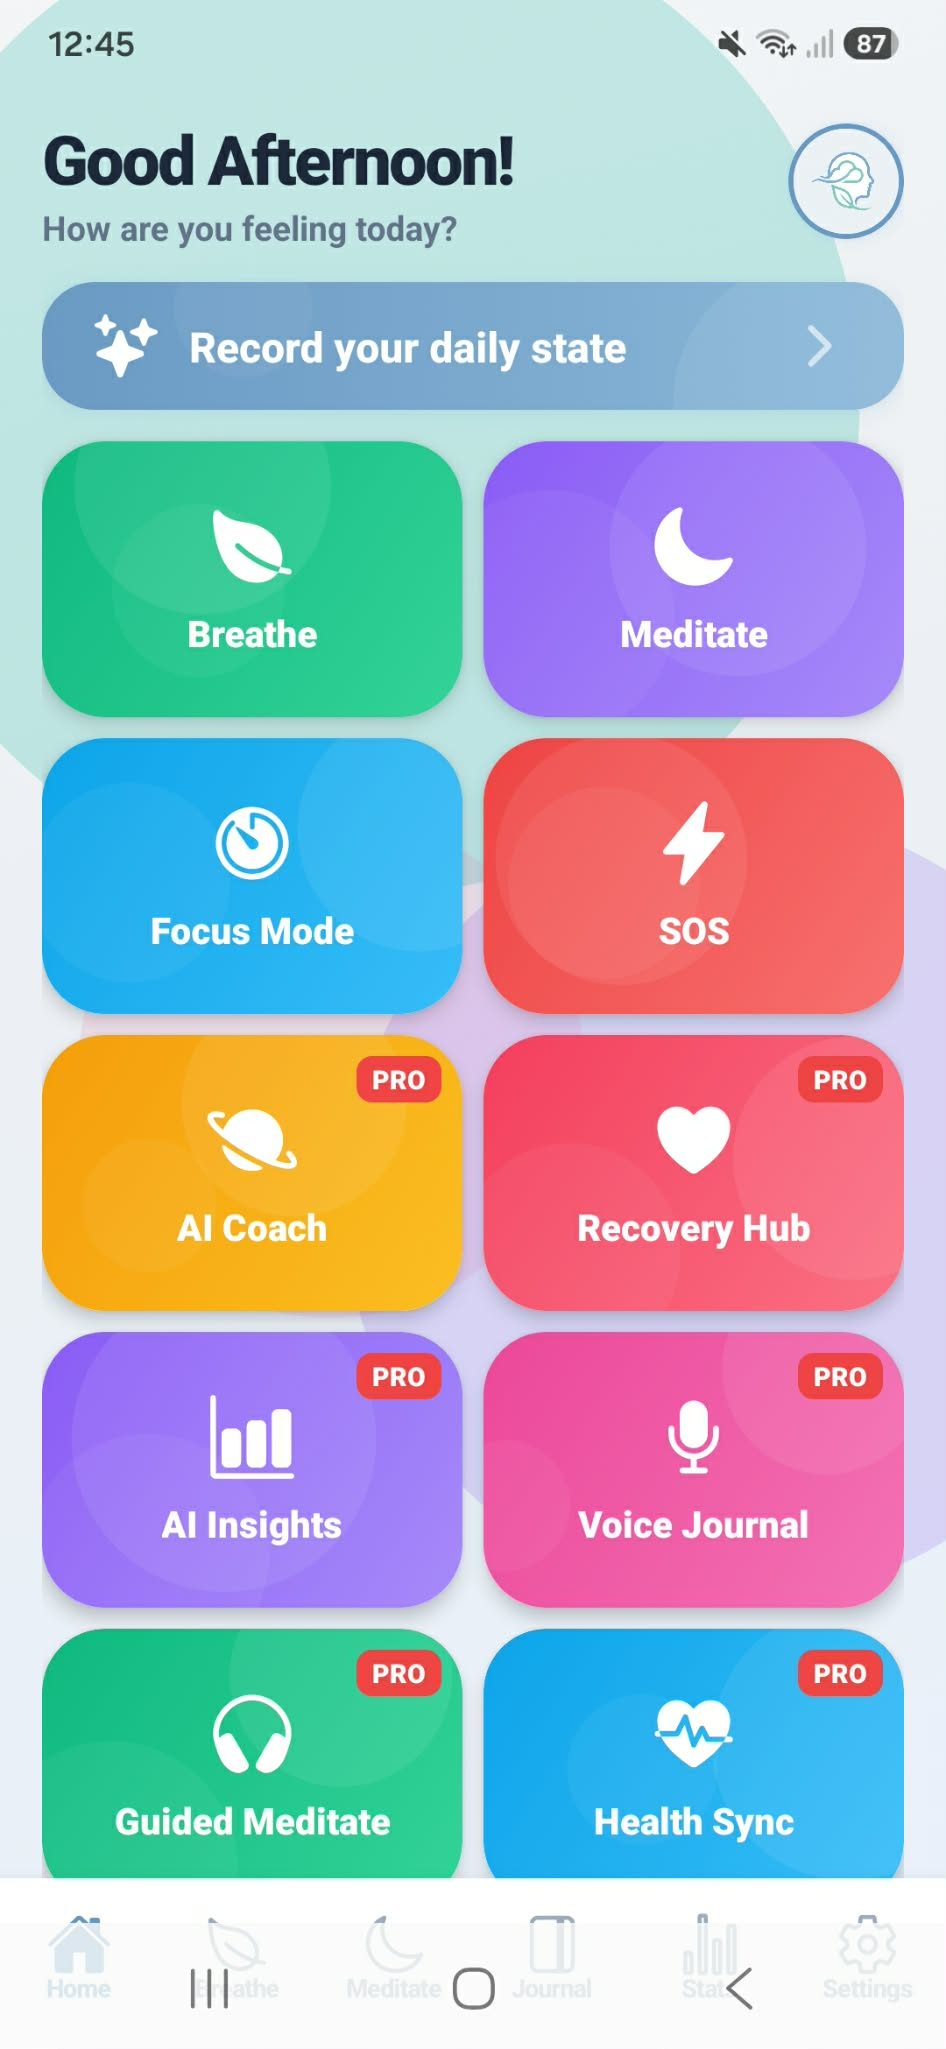
\includegraphics[width=\linewidth]{../graphics/burnoutfree/BurnoutFree1}
    \end{minipage}
    \hfill
    \begin{minipage}{0.3\textwidth}
        \centering
        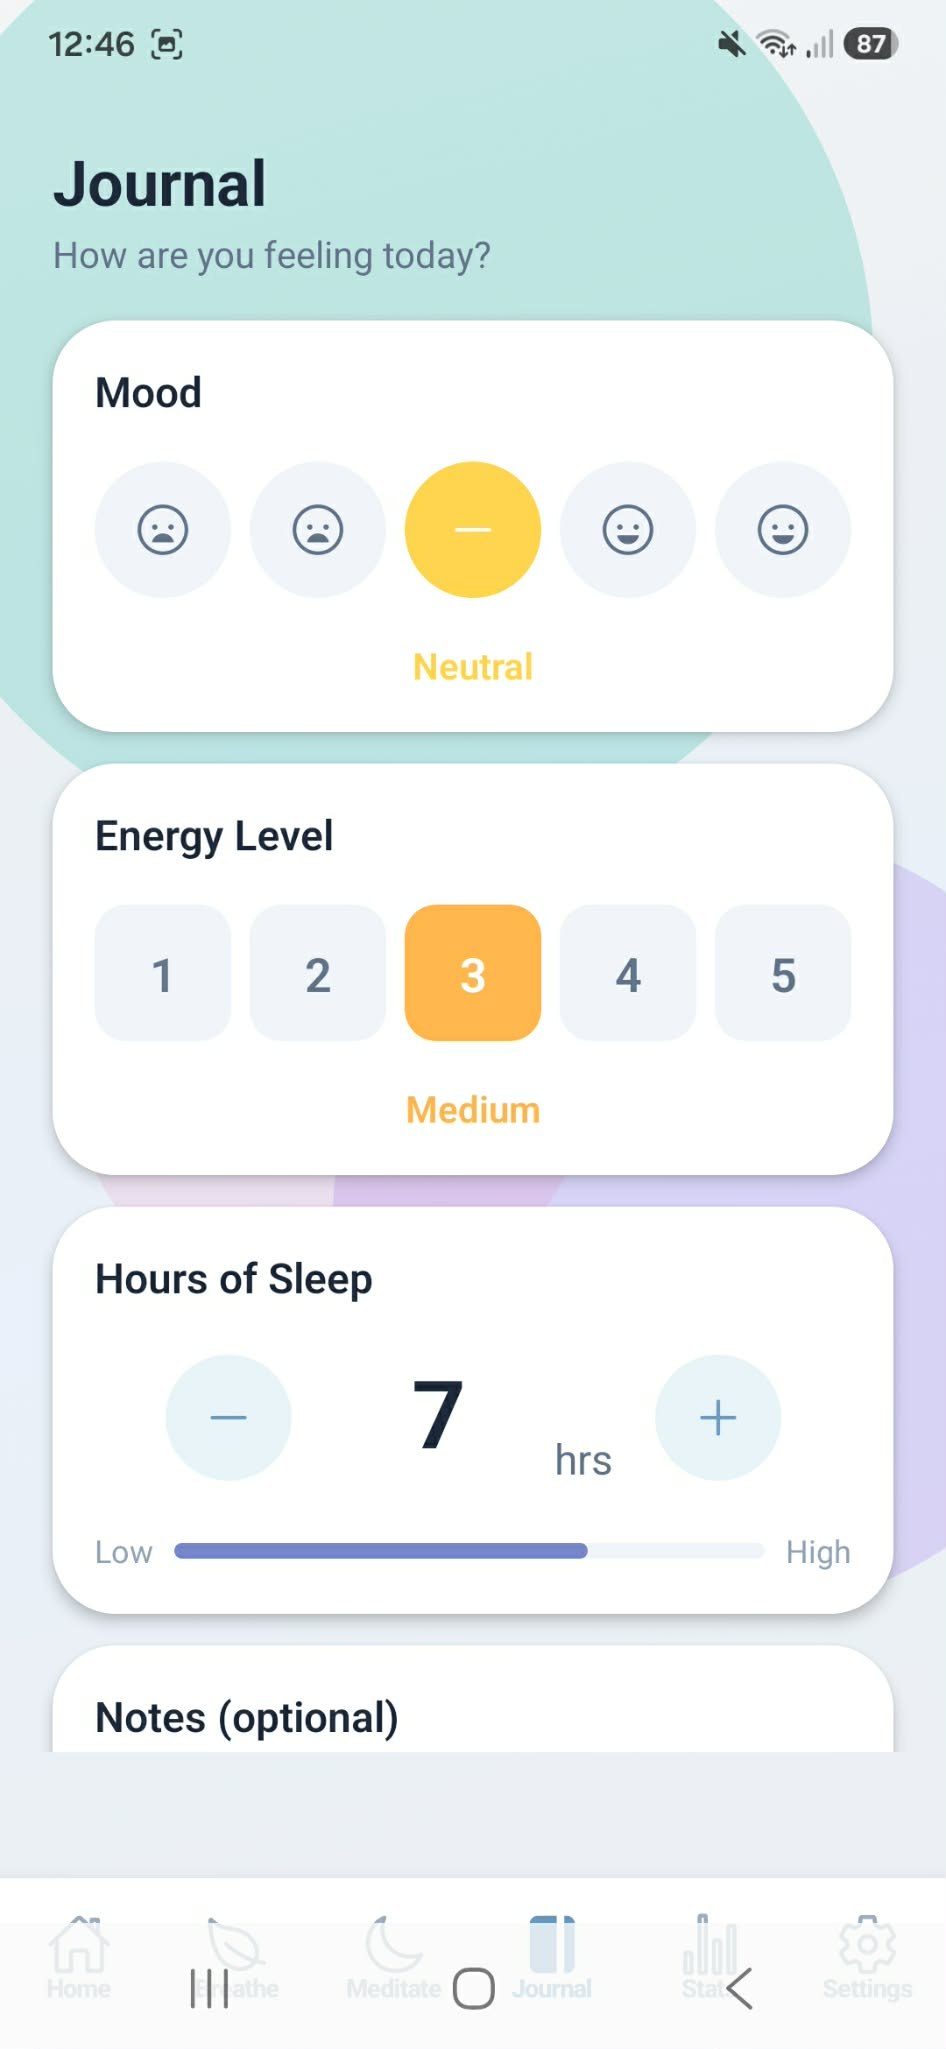
\includegraphics[width=\linewidth]{../graphics/burnoutfree/BurnoutFree6}
    \end{minipage}
    \hfill
    \begin{minipage}{0.3\textwidth}
        \centering
        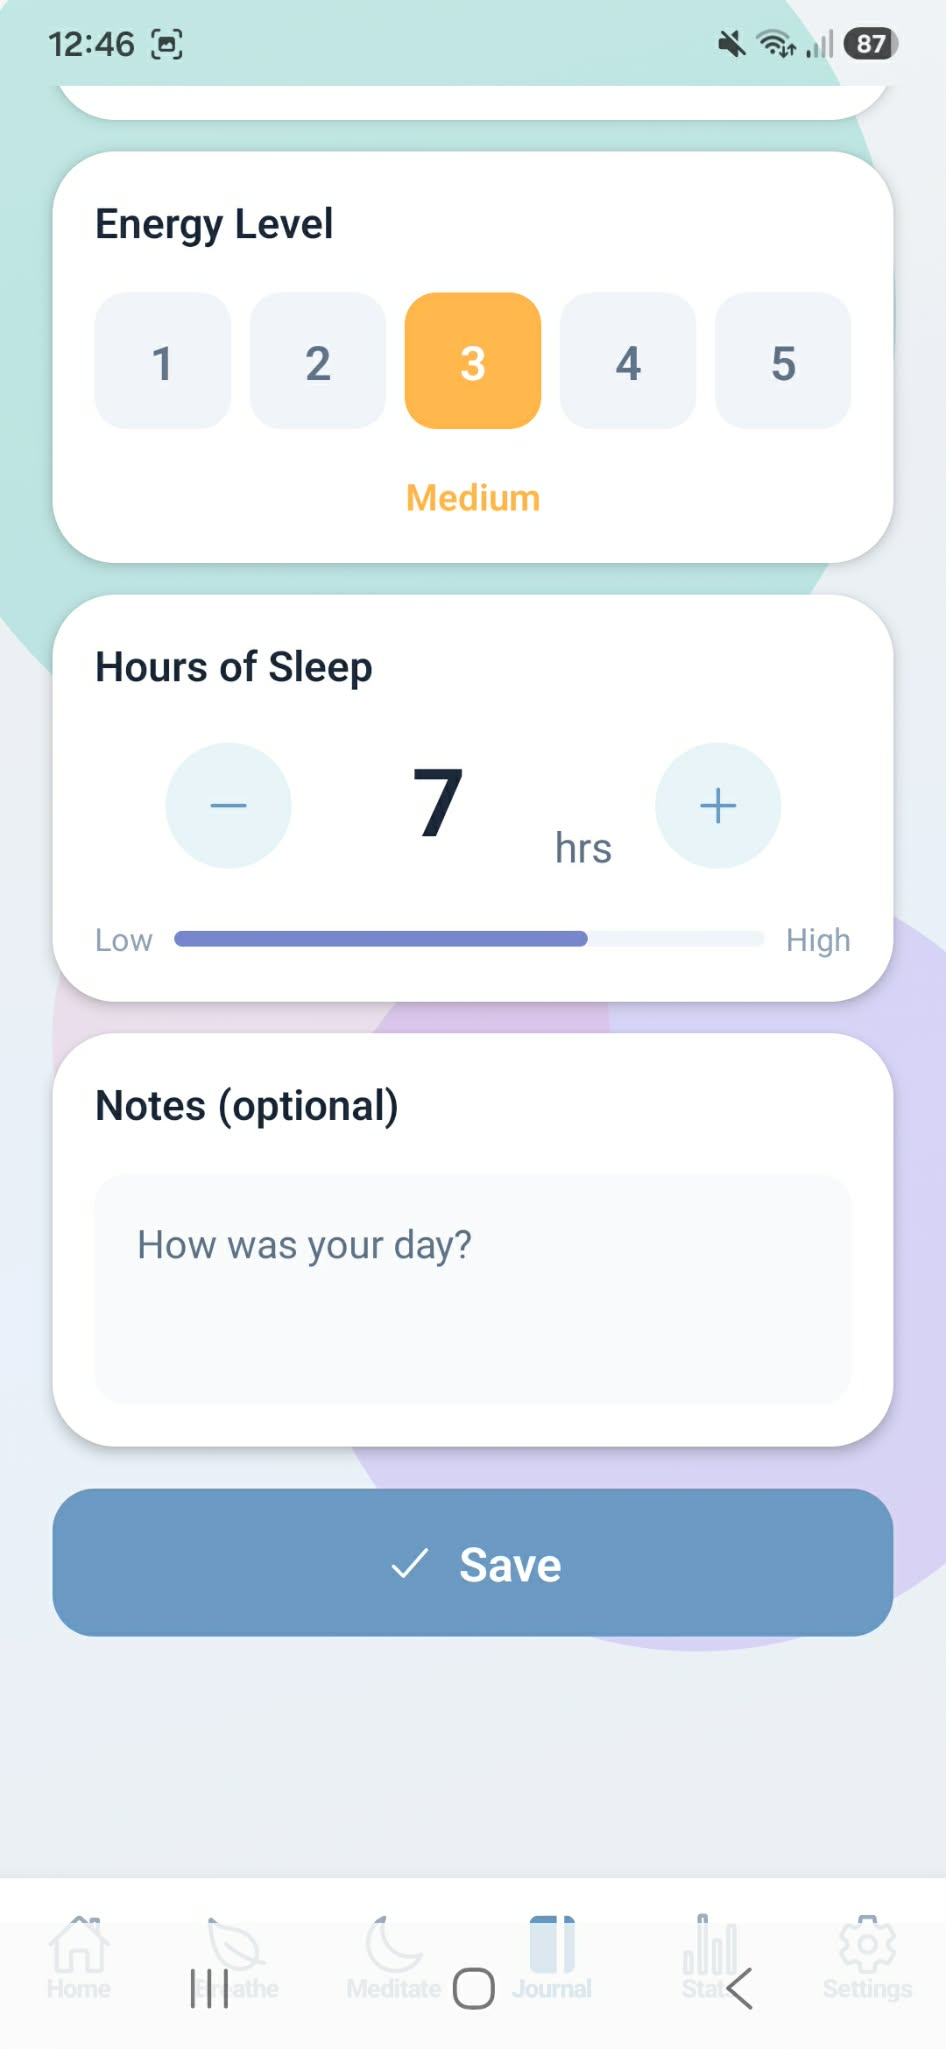
\includegraphics[width=\linewidth]{../graphics/burnoutfree/BurnoutFree7}
    \end{minipage}
    
    \caption{De homepagina (links) en de dagboekpagina (midden en rechts).}
    \label{fig:burnout-free-1}
\end{figure}

\begin{figure}[H]
    \centering
    
    \begin{minipage}{0.3\textwidth}
        \centering
        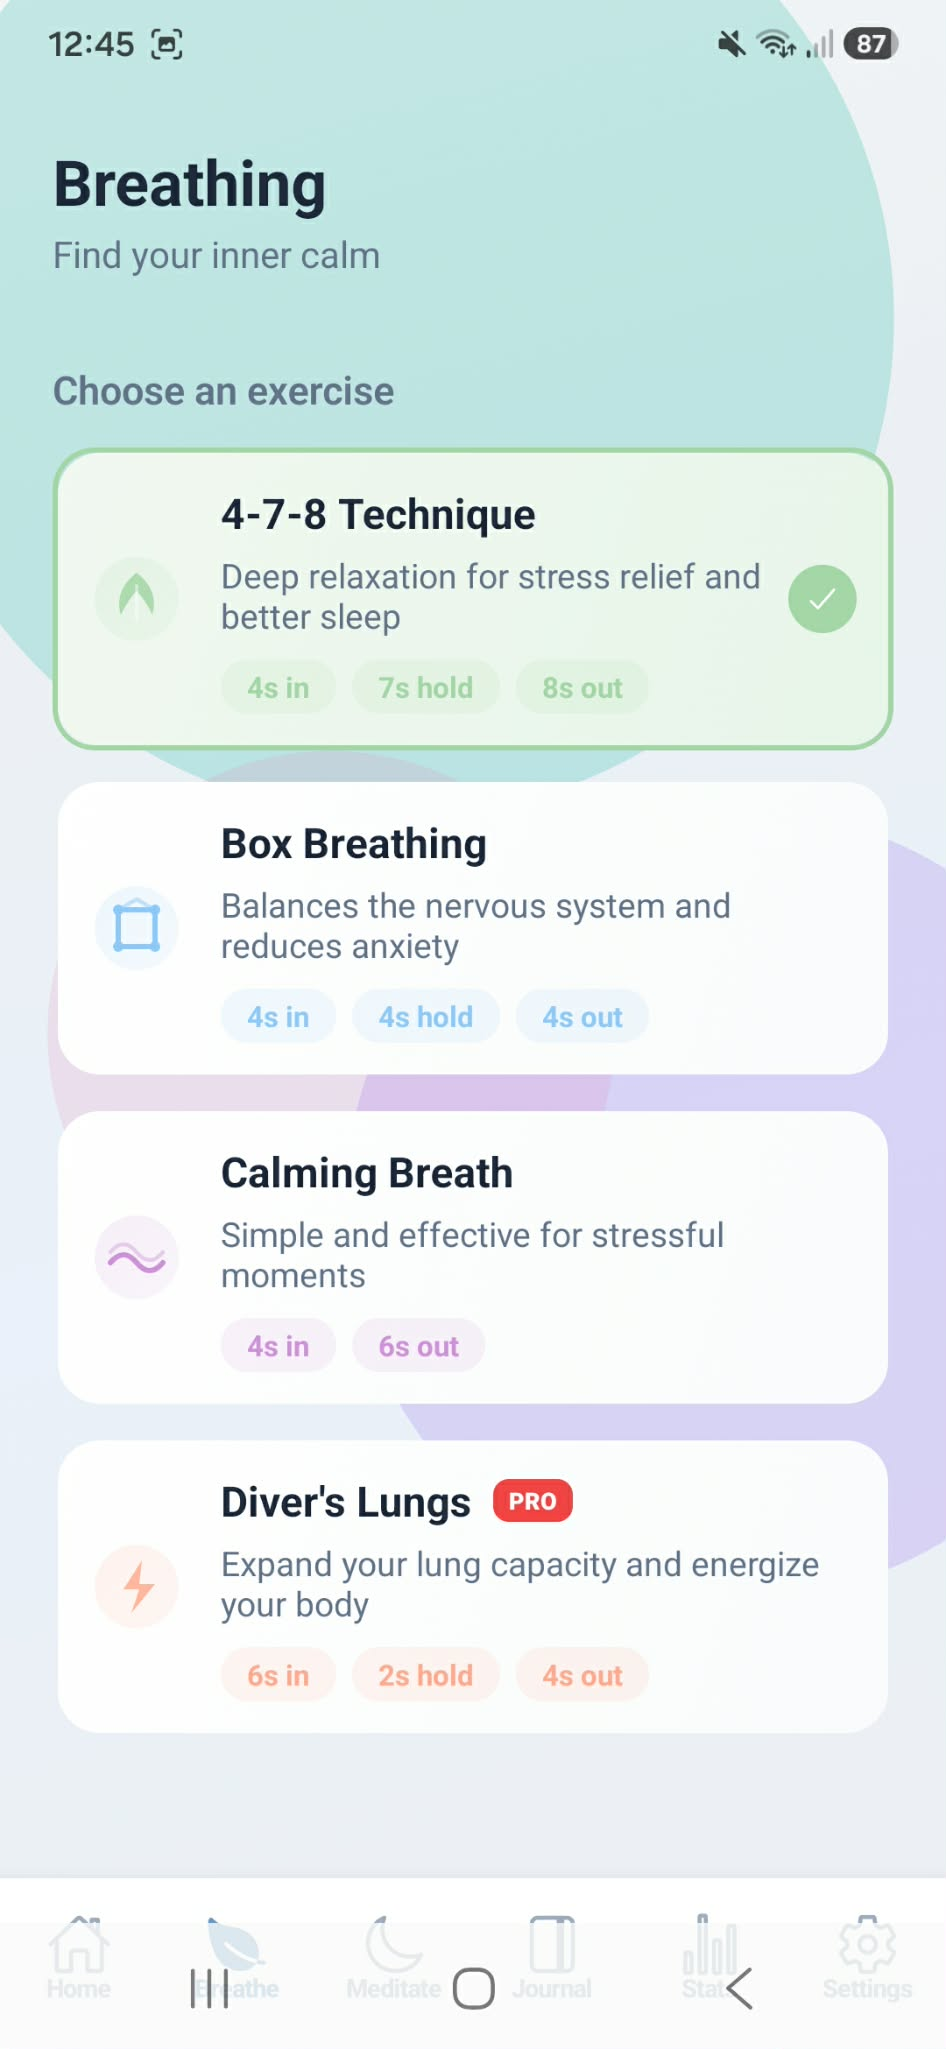
\includegraphics[width=\linewidth]{../graphics/burnoutfree/BurnoutFree2}
    \end{minipage}
    \hfill
    \begin{minipage}{0.3\textwidth}
        \centering
        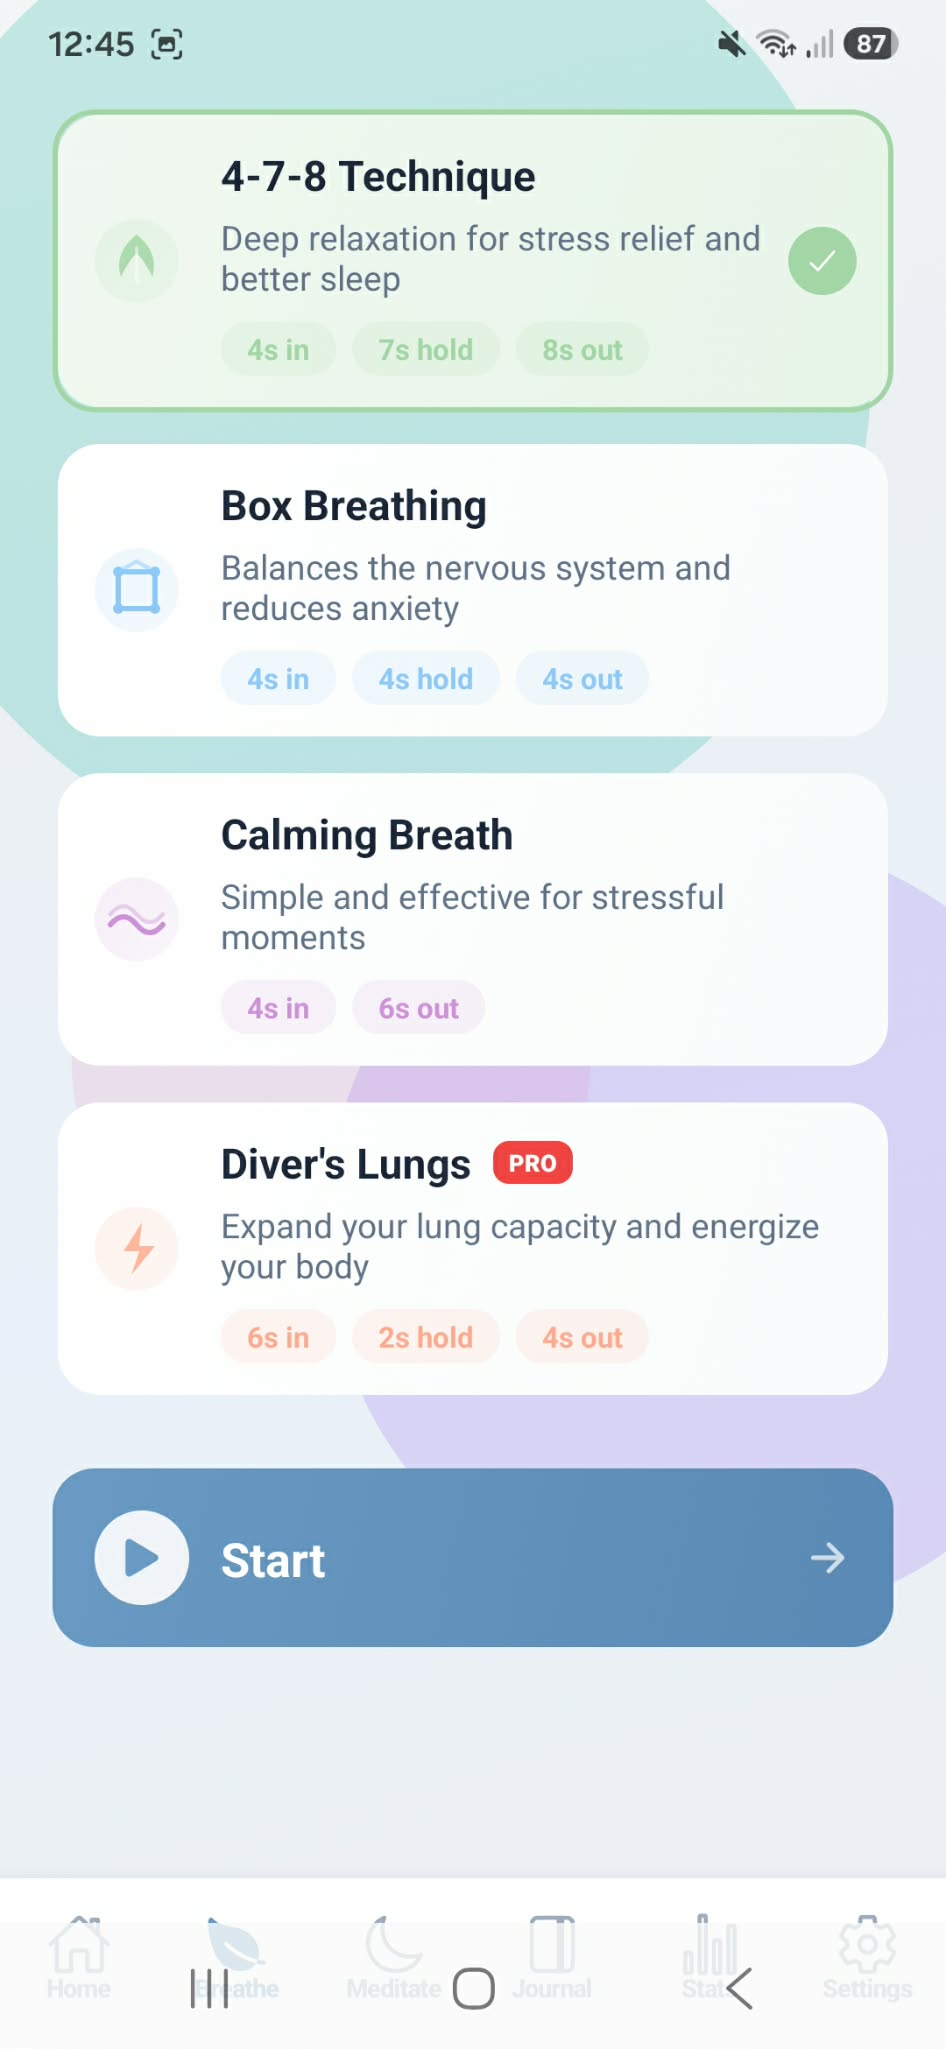
\includegraphics[width=\linewidth]{../graphics/burnoutfree/BurnoutFree3}
    \end{minipage}
    \hfill
    \begin{minipage}{0.3\textwidth}
        \centering
        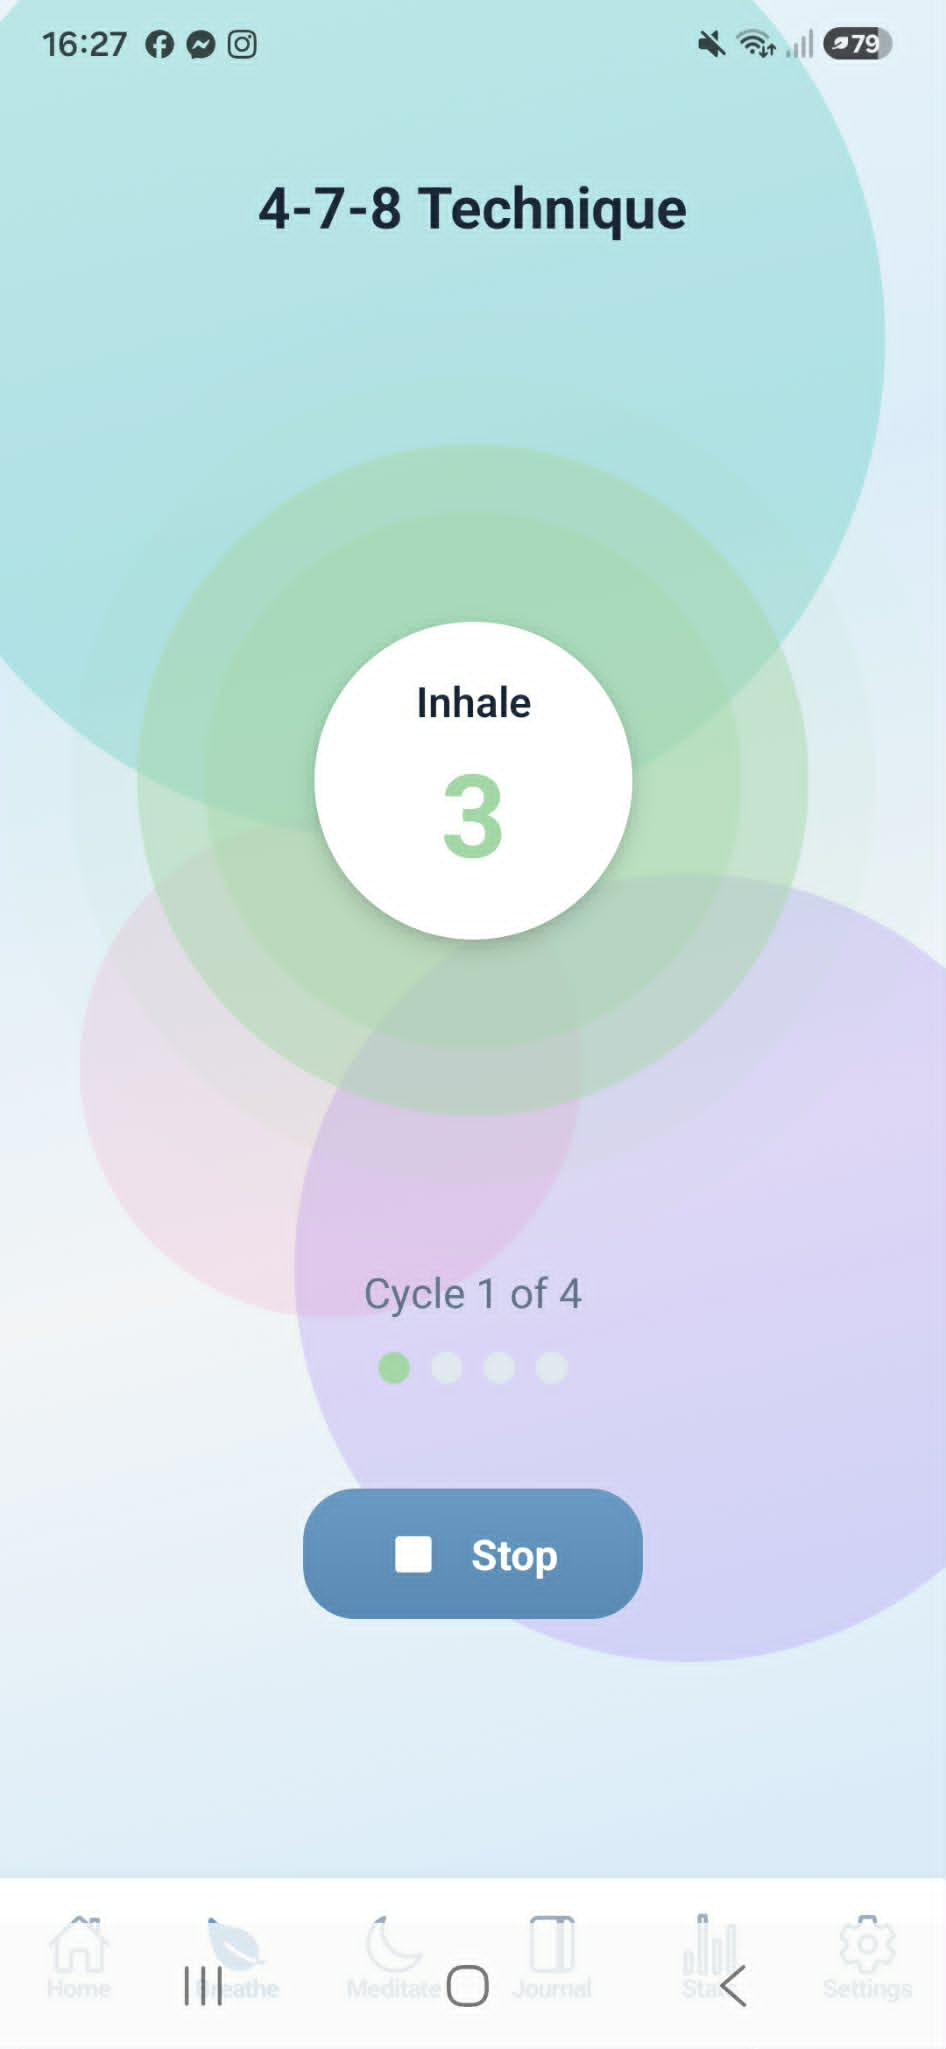
\includegraphics[width=\linewidth]{../graphics/burnoutfree/BurnoutFree15}
    \end{minipage}
    
    \caption{De ademhalingsoefeningen met vier beschikbare technieken.}
    \label{fig:burnout-free-2}
\end{figure}

\begin{figure}[H]
    \centering
    
    \begin{minipage}{0.3\textwidth}
        \centering
        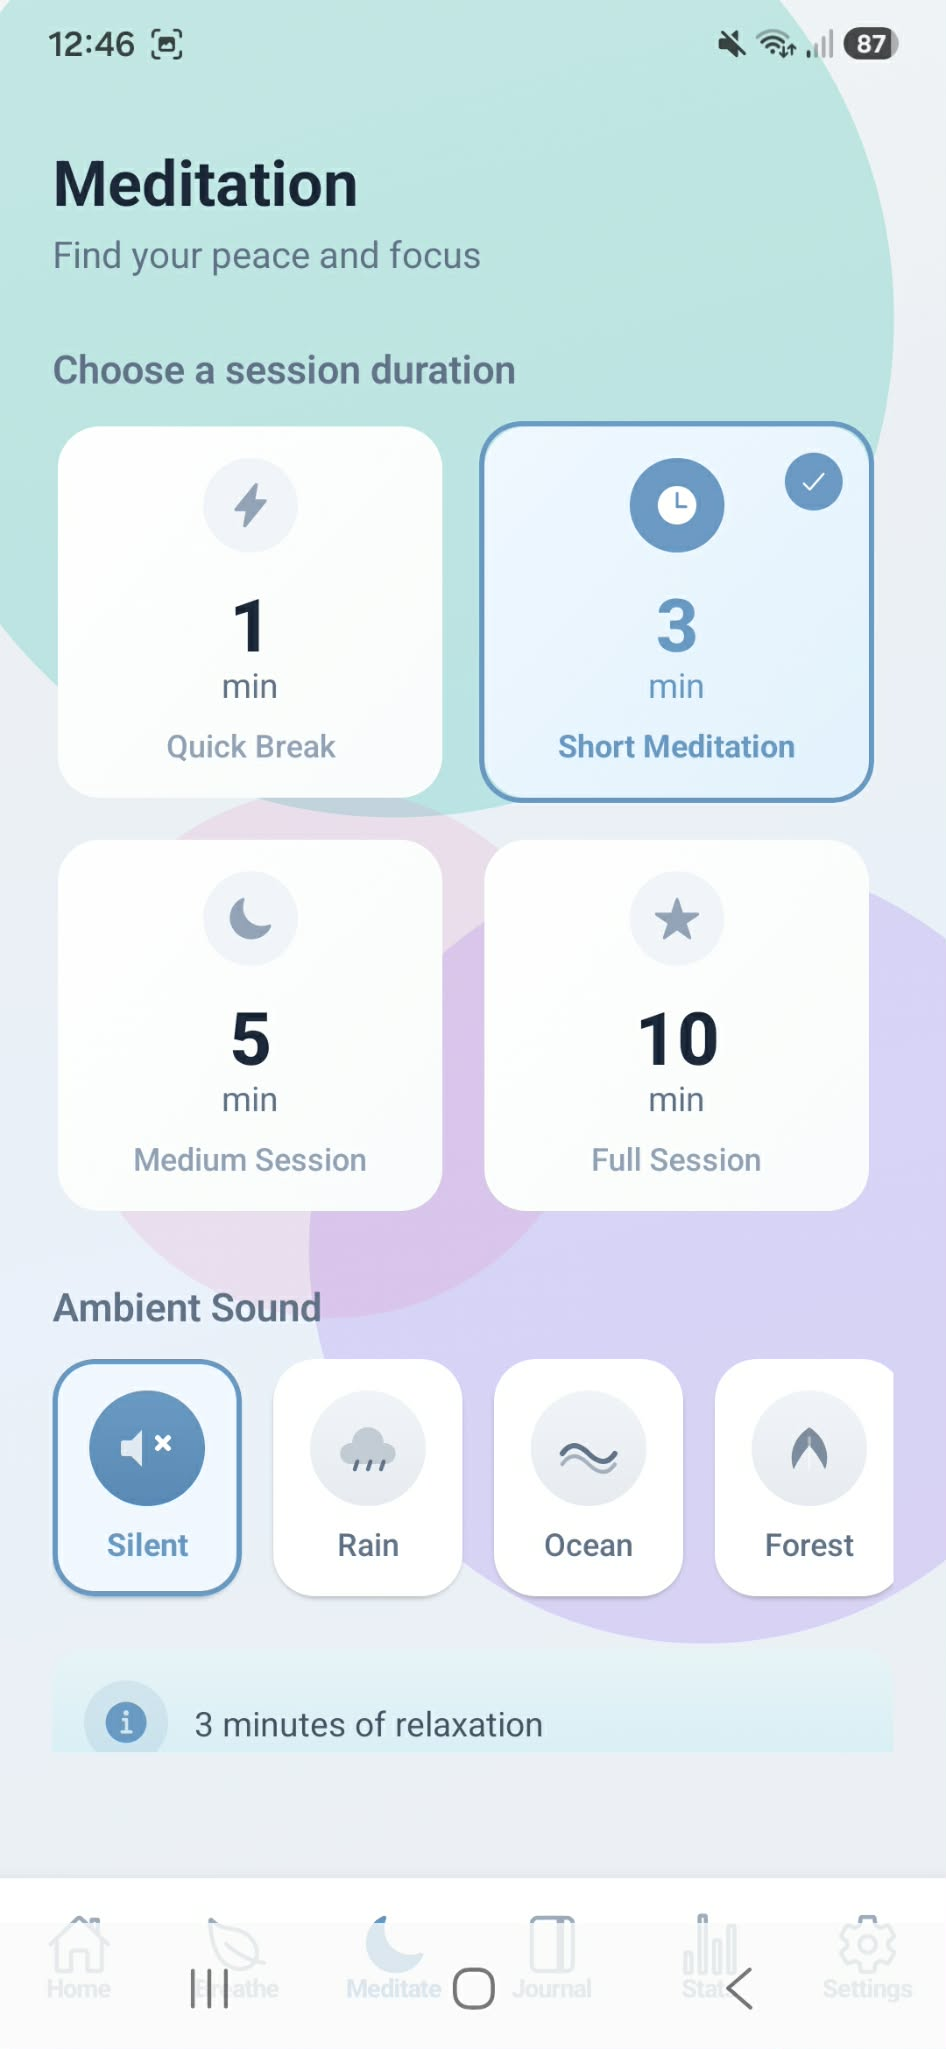
\includegraphics[width=\linewidth]{../graphics/burnoutfree/BurnoutFree4}
    \end{minipage}
    \hfill
    \begin{minipage}{0.3\textwidth}
        \centering
        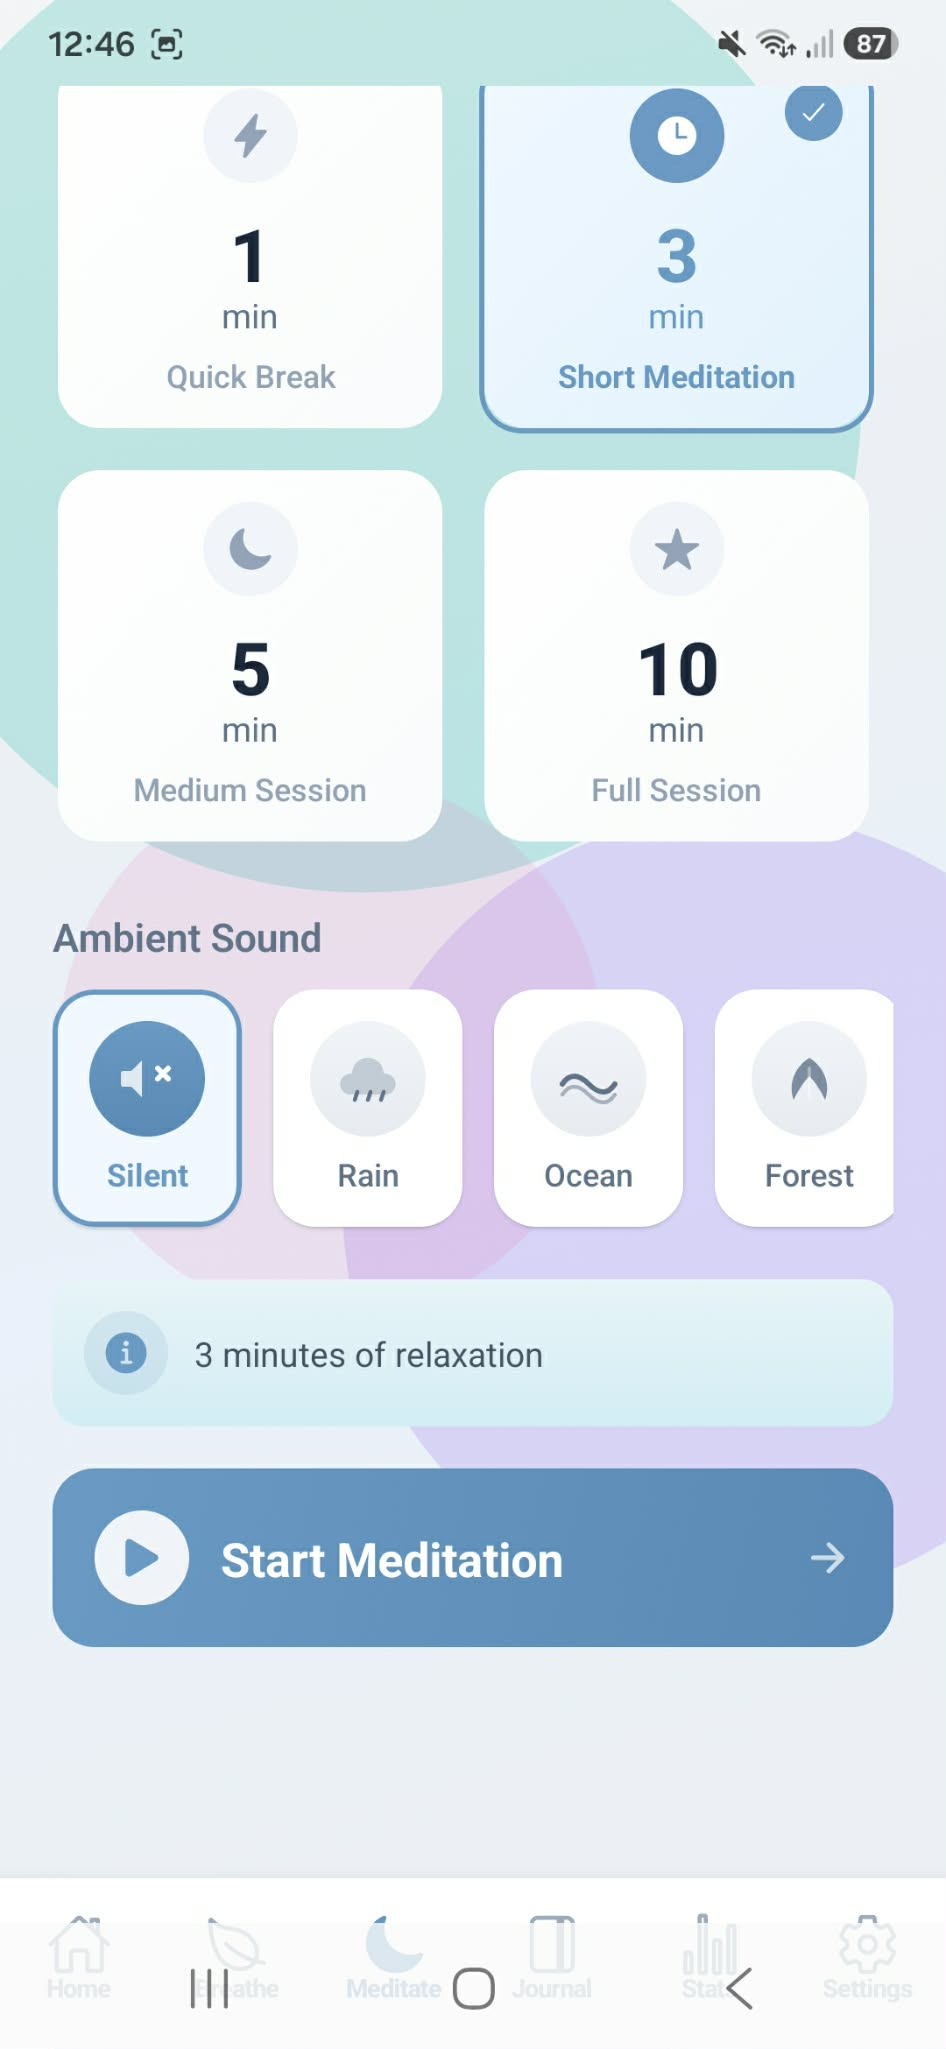
\includegraphics[width=\linewidth]{../graphics/burnoutfree/BurnoutFree5}
    \end{minipage}
    \hfill
    \begin{minipage}{0.3\textwidth}
        \centering
        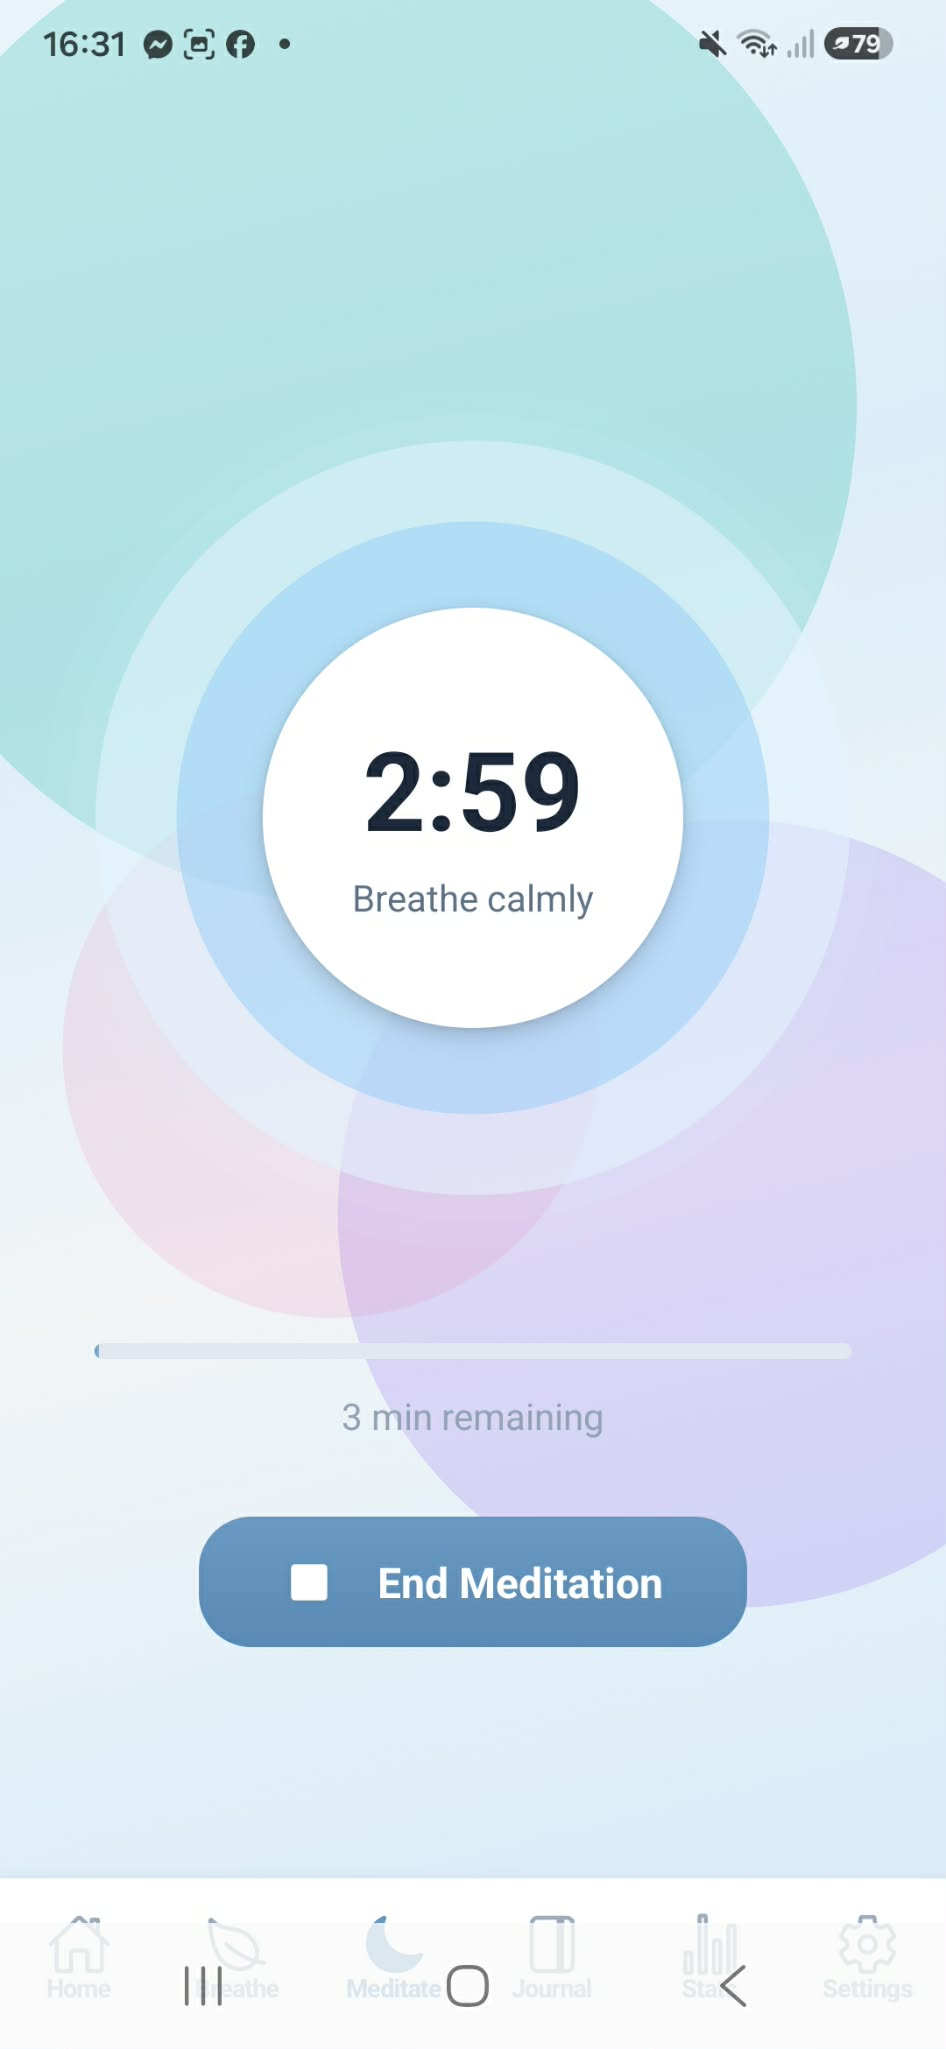
\includegraphics[width=\linewidth]{../graphics/burnoutfree/BurnoutFree16}
    \end{minipage}
    
    \caption{De meditatiesessies met vier beschikbare duraties.}
    \label{fig:burnout-free-3}
\end{figure}

\begin{figure}[H]
    \centering
    
    \begin{minipage}{0.3\textwidth}
        \centering
        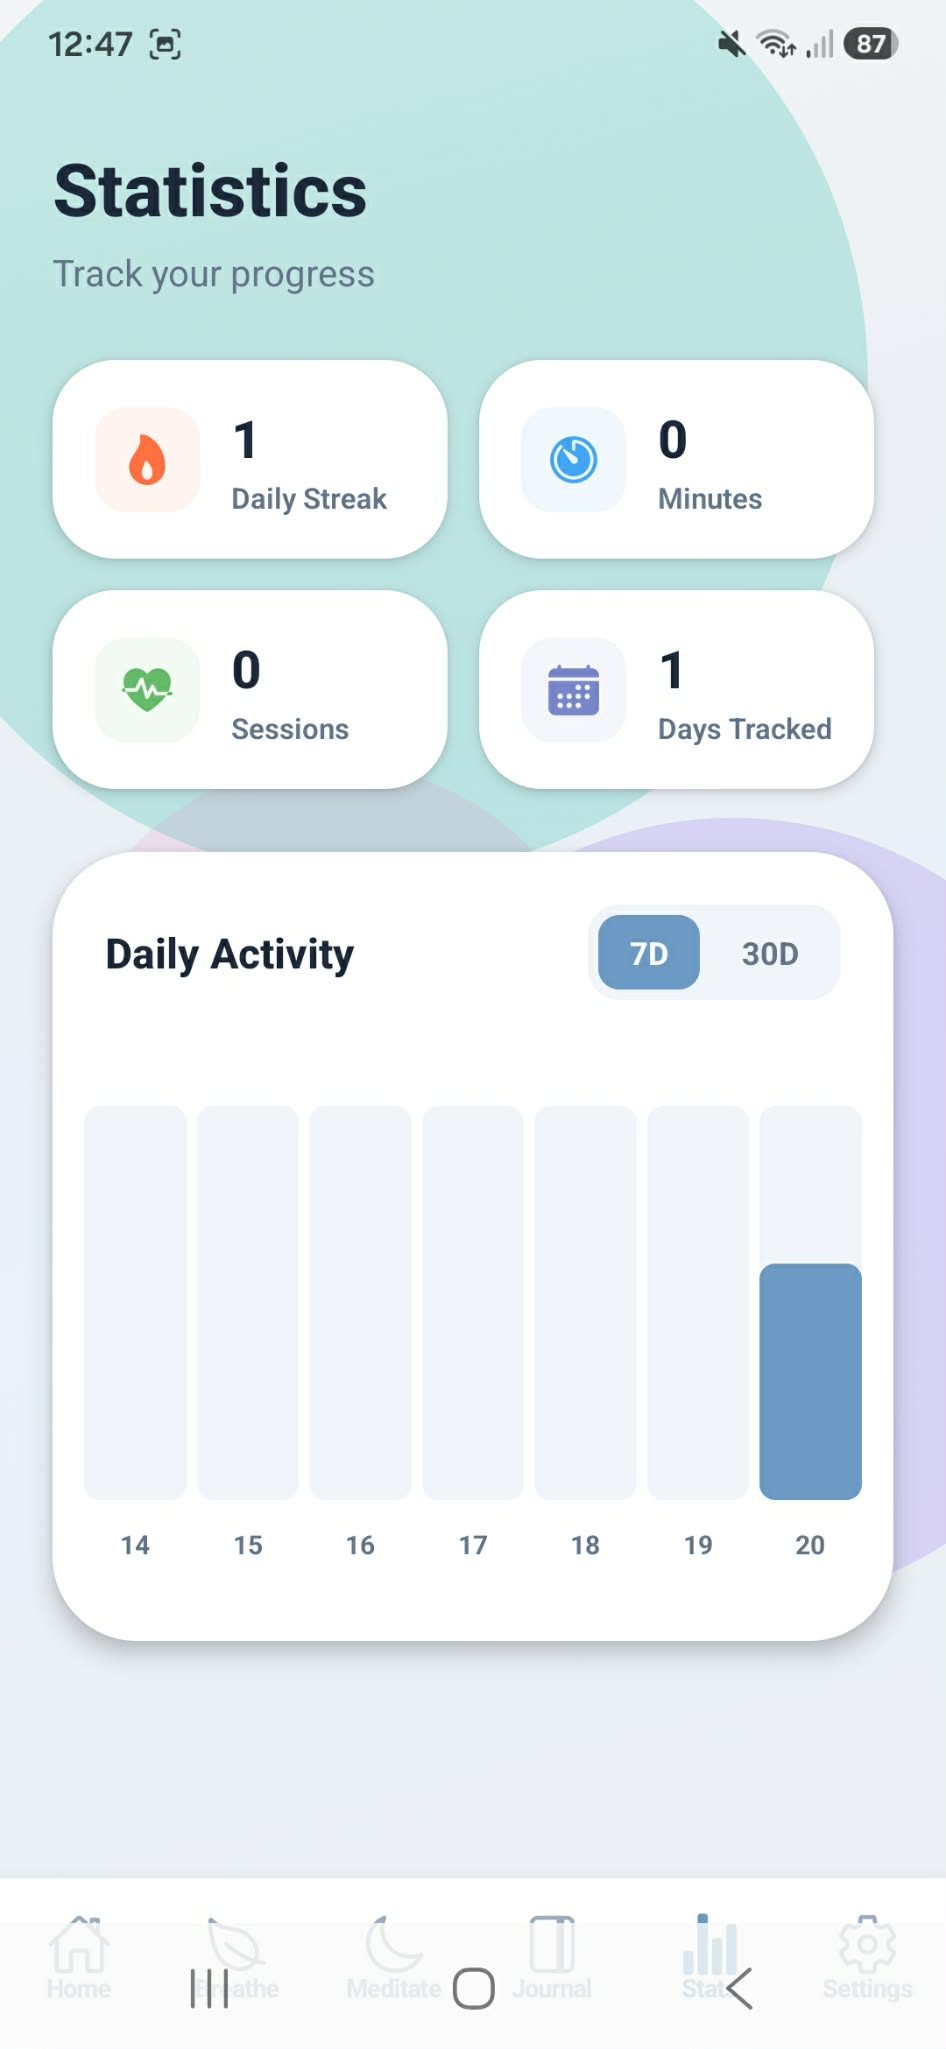
\includegraphics[width=\linewidth]{../graphics/burnoutfree/BurnoutFree8}
    \end{minipage}
    \hfill
    \begin{minipage}{0.3\textwidth}
        \centering
        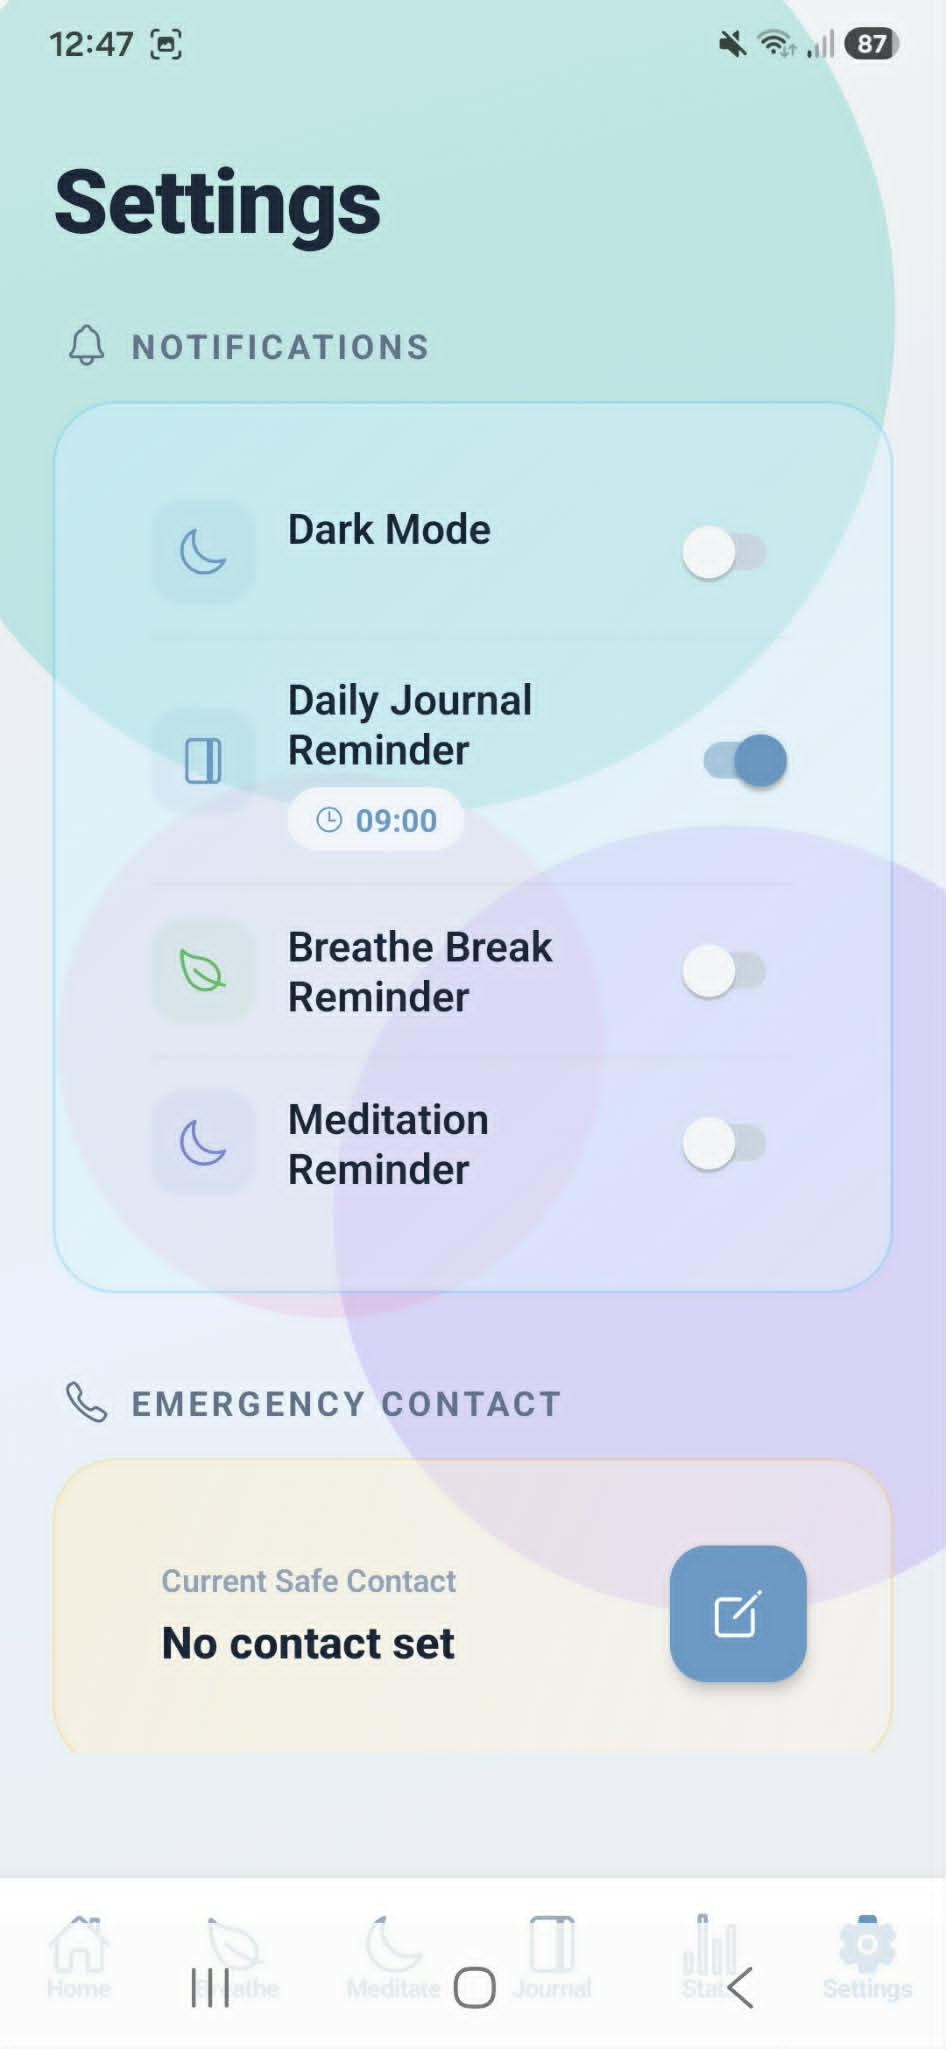
\includegraphics[width=\linewidth]{../graphics/burnoutfree/BurnoutFree9}
    \end{minipage}
    \hfill
    \begin{minipage}{0.3\textwidth}
        \centering
        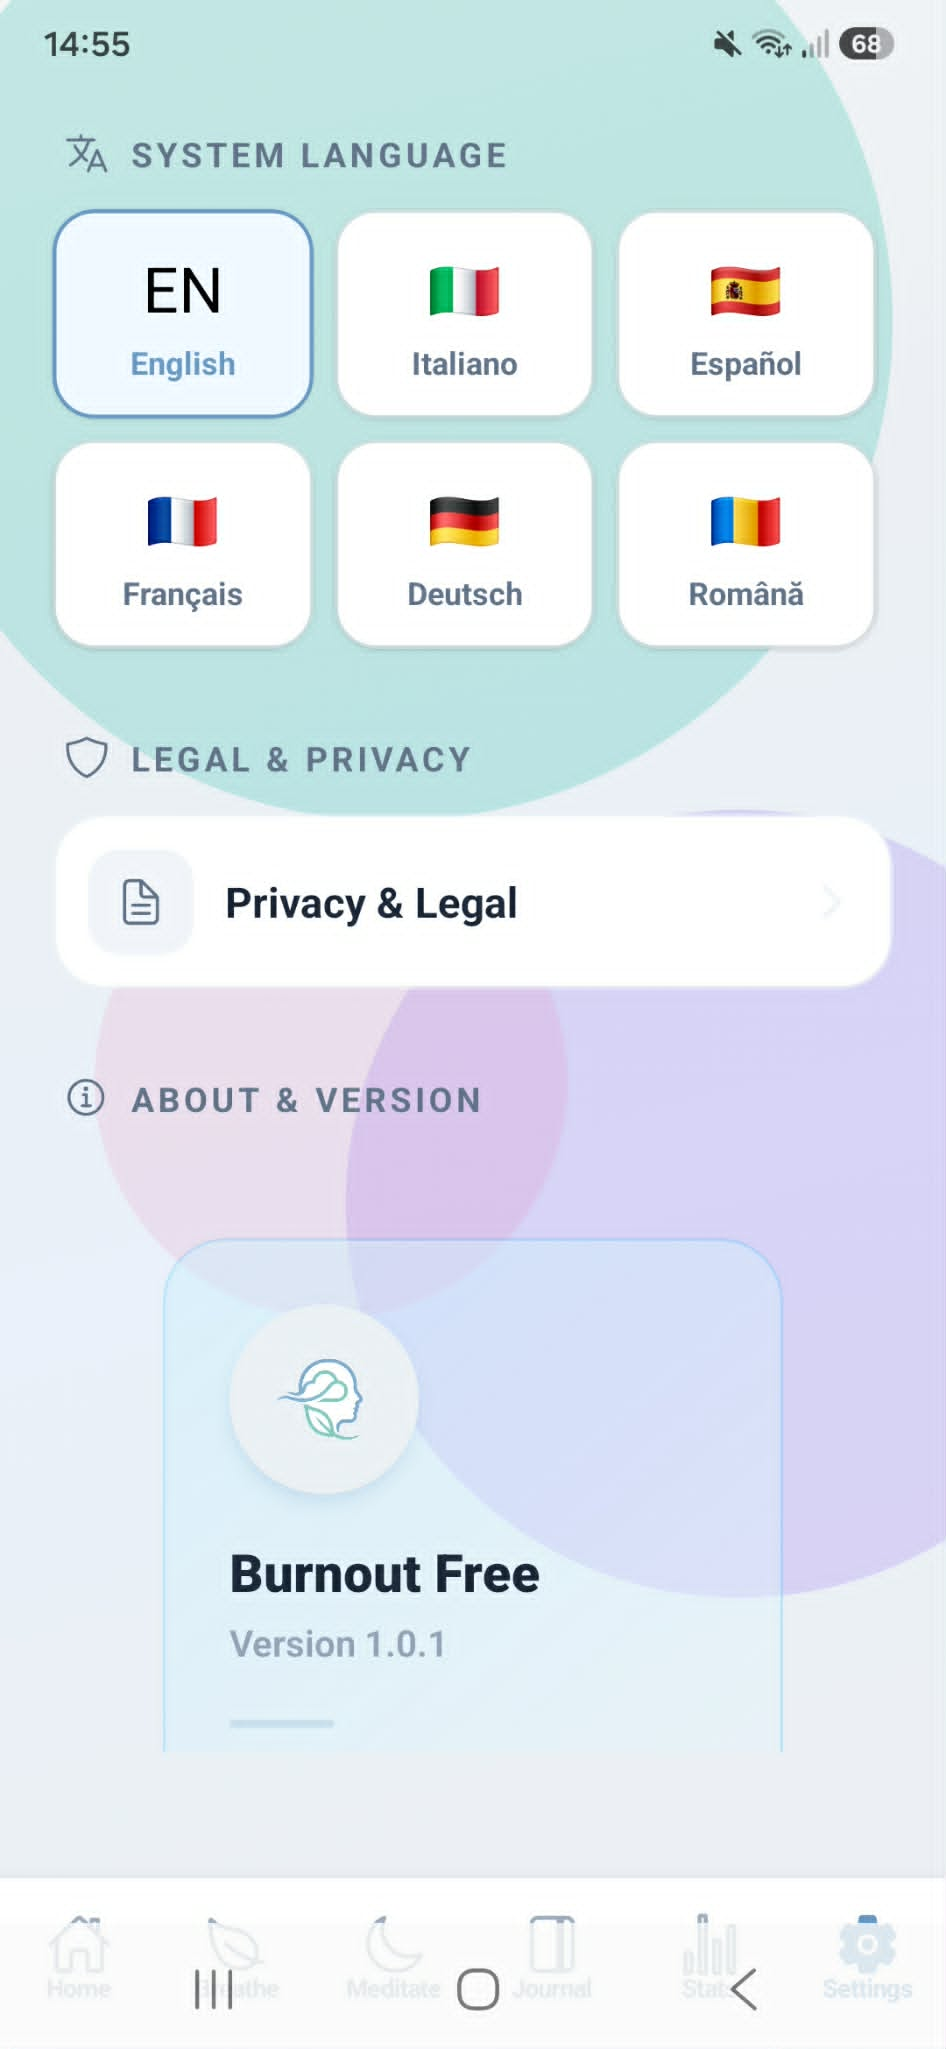
\includegraphics[width=\linewidth]{../graphics/burnoutfree/BurnoutFree14}
    \end{minipage}
    
    \caption{De statistiekenpagina (links) en de instellingenpagina (midden en rechts).}
    \label{fig:burnout-free-4}
\end{figure}

\begin{figure}[H]
    \centering
    
    \begin{minipage}{0.3\textwidth}
        \centering
        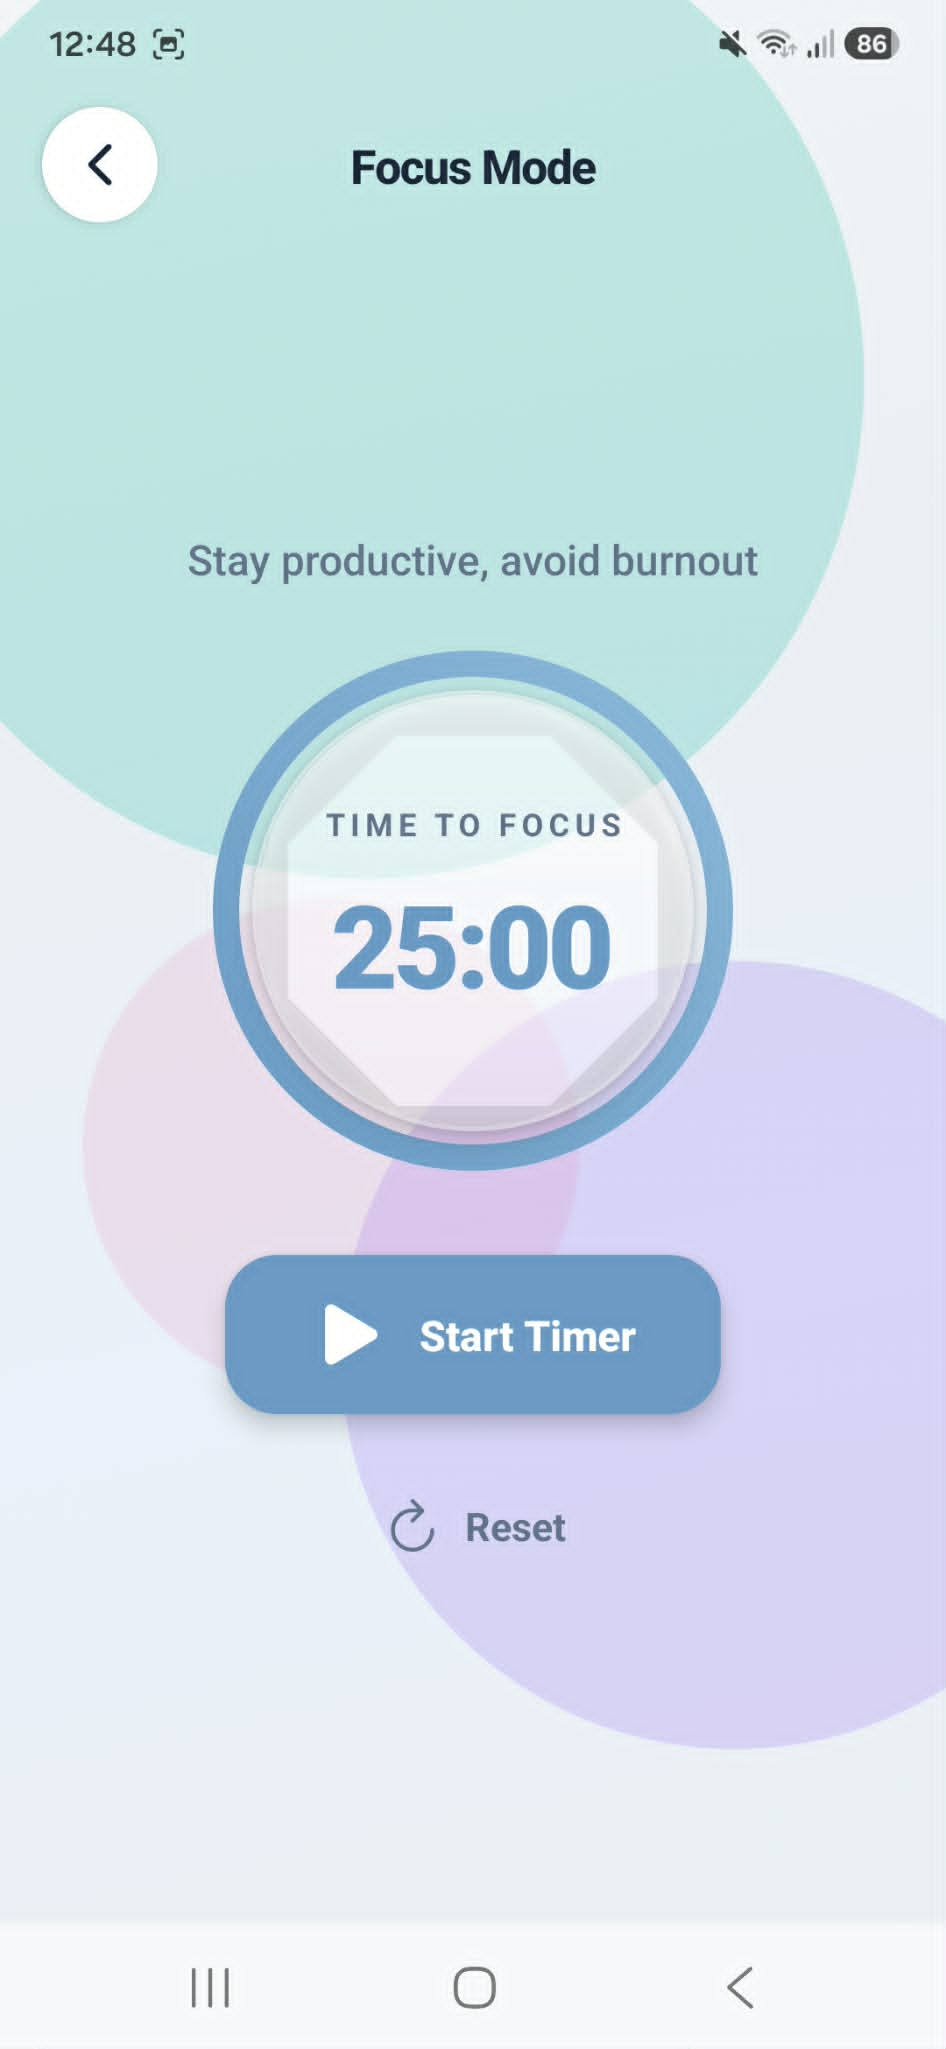
\includegraphics[width=\linewidth]{../graphics/burnoutfree/BurnoutFree11}
    \end{minipage}
    \hfill
    \begin{minipage}{0.3\textwidth}
        \centering
        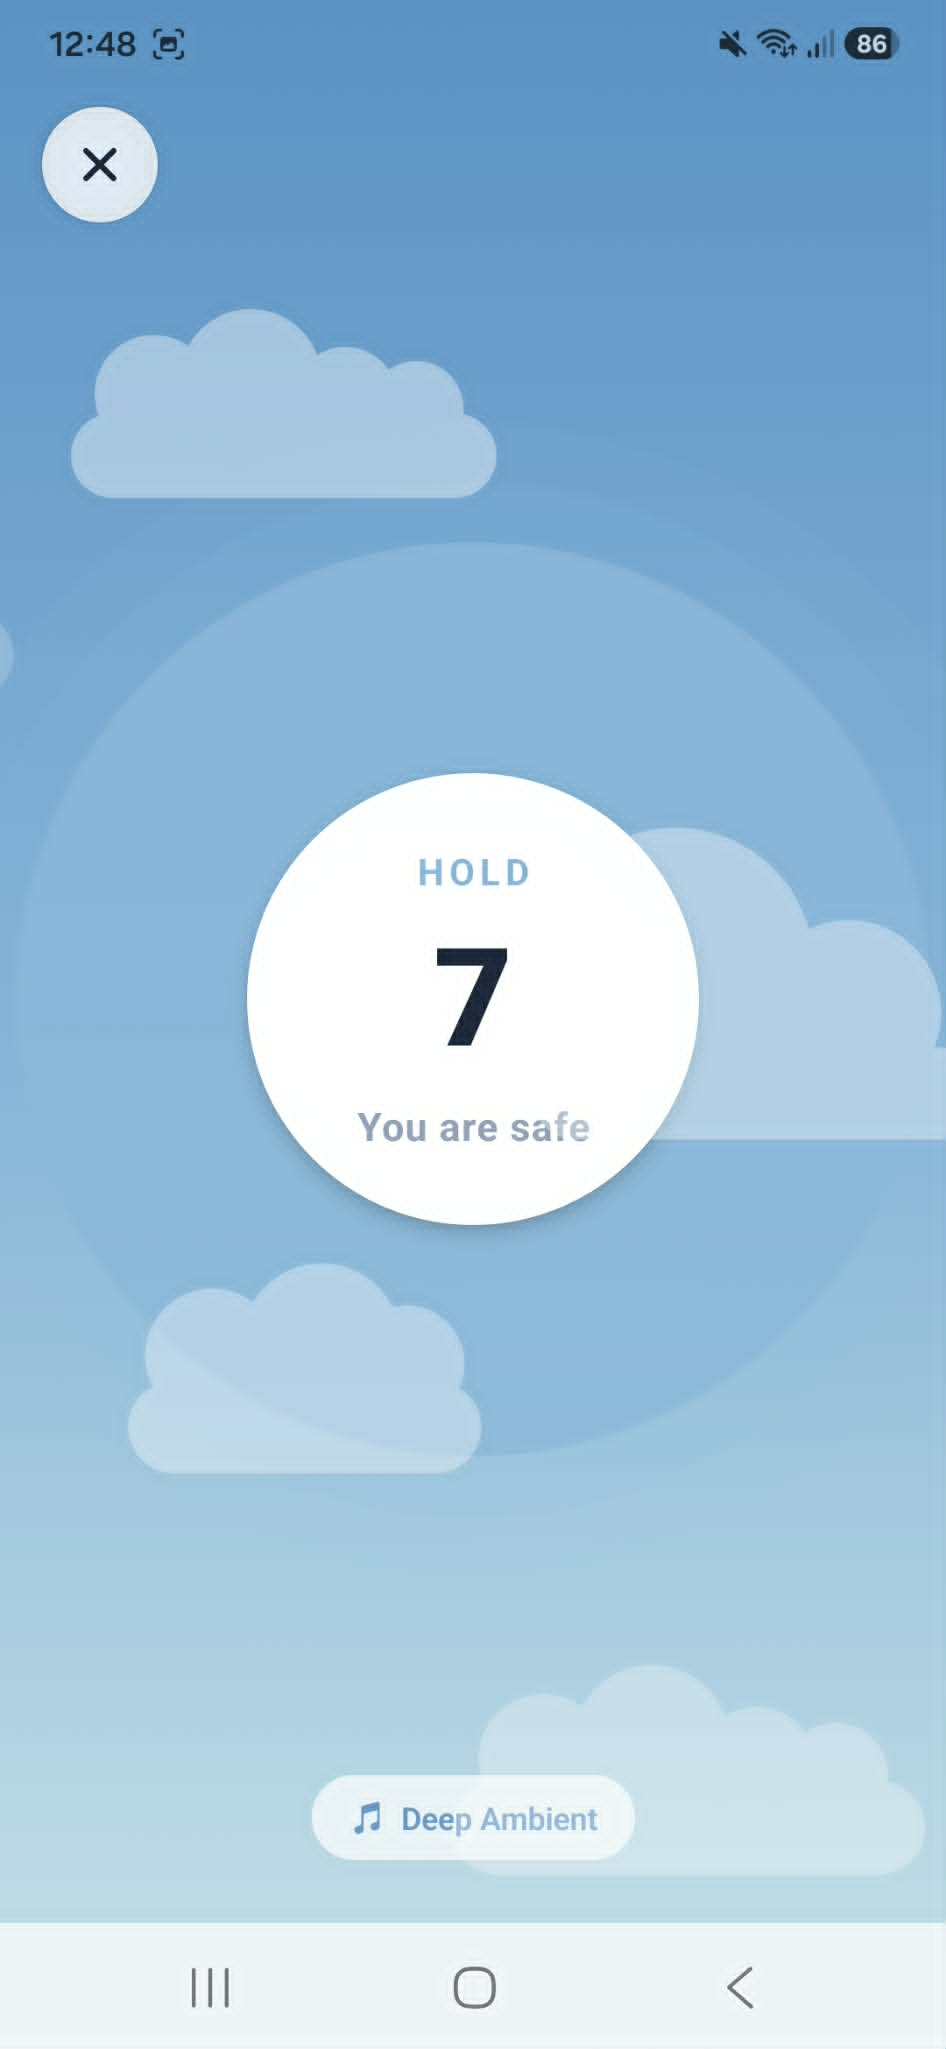
\includegraphics[width=\linewidth]{../graphics/burnoutfree/BurnoutFree12}
    \end{minipage}
    \hfill
    \begin{minipage}{0.3\textwidth}
        \centering
        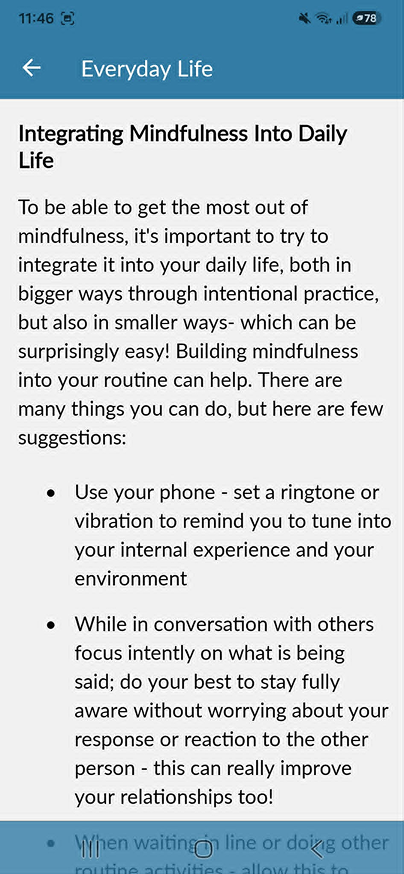
\includegraphics[width=\linewidth]{../graphics/burnoutfree/MindfulnessCoach1}
    \end{minipage}

    \caption{Focus modus (links) en SOS modus (midden) van Burnout Free, met een voorbeeld van kenniscontent uit Mindfulness Coach (rechts).}
    \label{fig:burnout-free-5}
\end{figure}

\begin{figure}[H]
    \centering
    
    \begin{minipage}{0.3\textwidth}
        \centering
        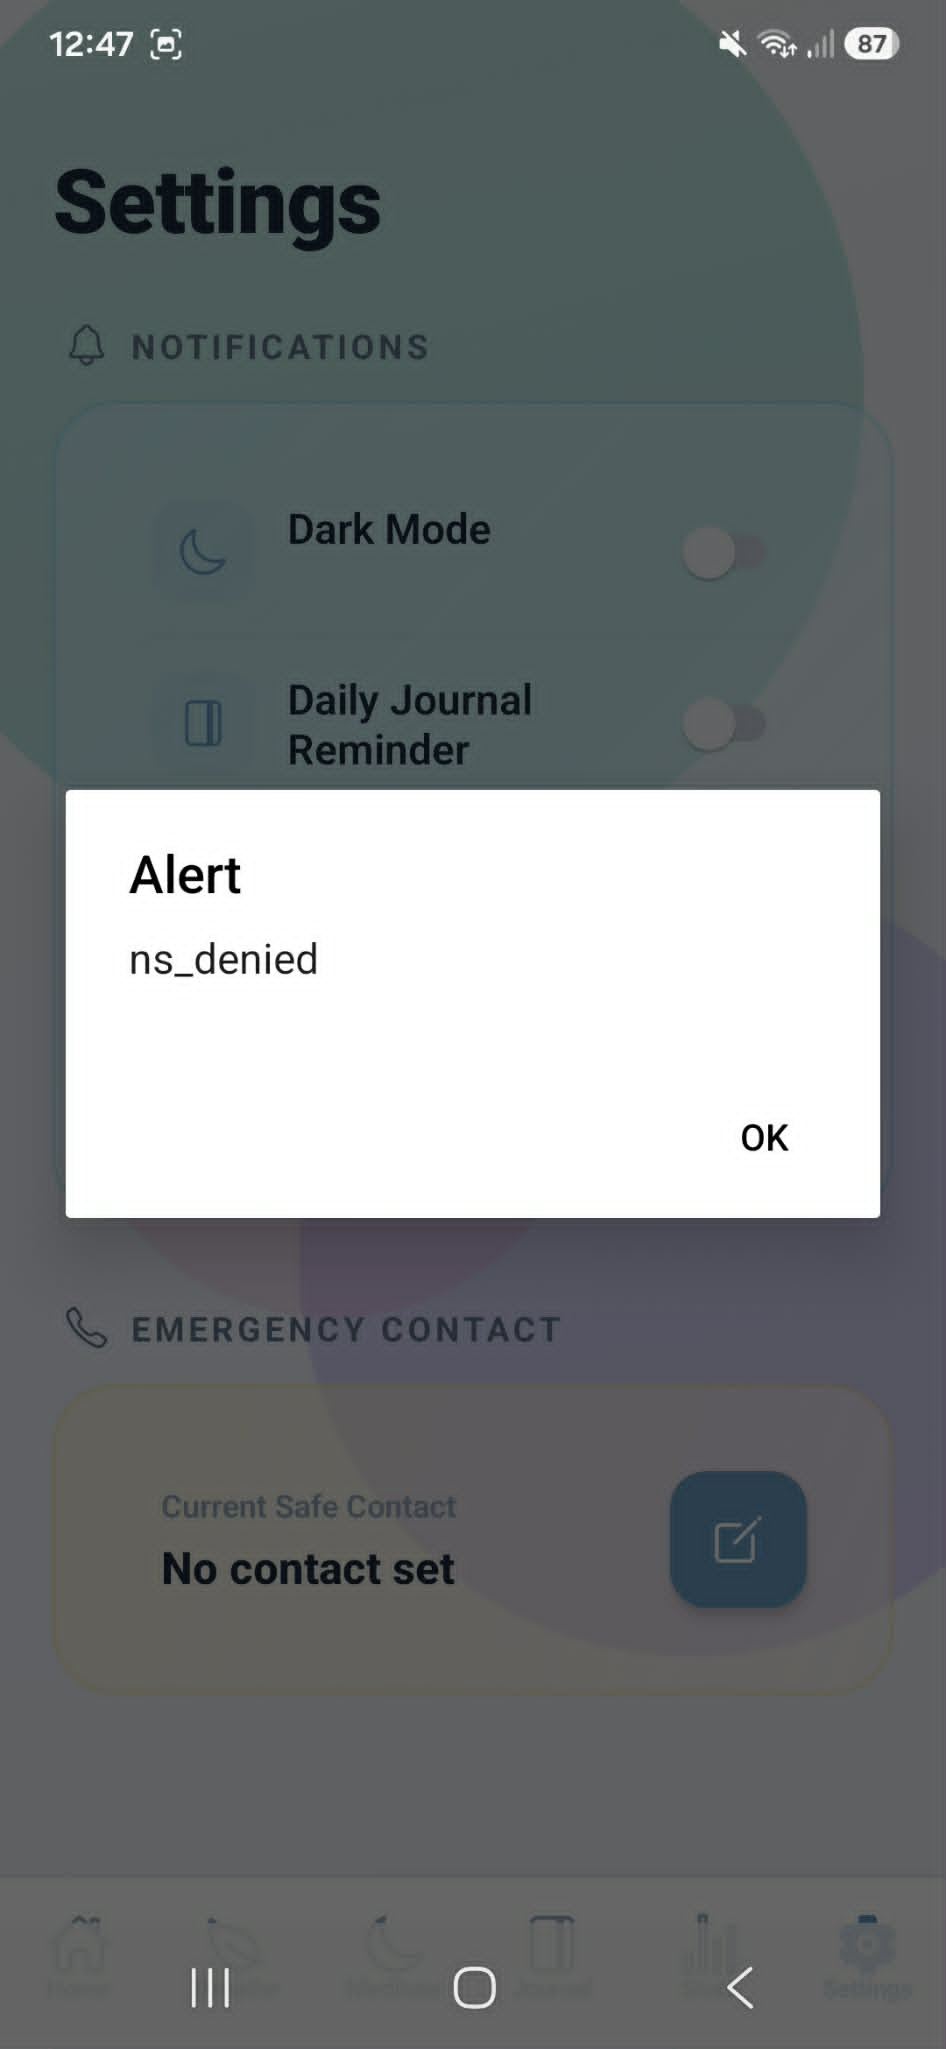
\includegraphics[width=\linewidth]{../graphics/burnoutfree/BurnoutFree10}
    \end{minipage}
    \hfill
    \begin{minipage}{0.3\textwidth}
        \centering
        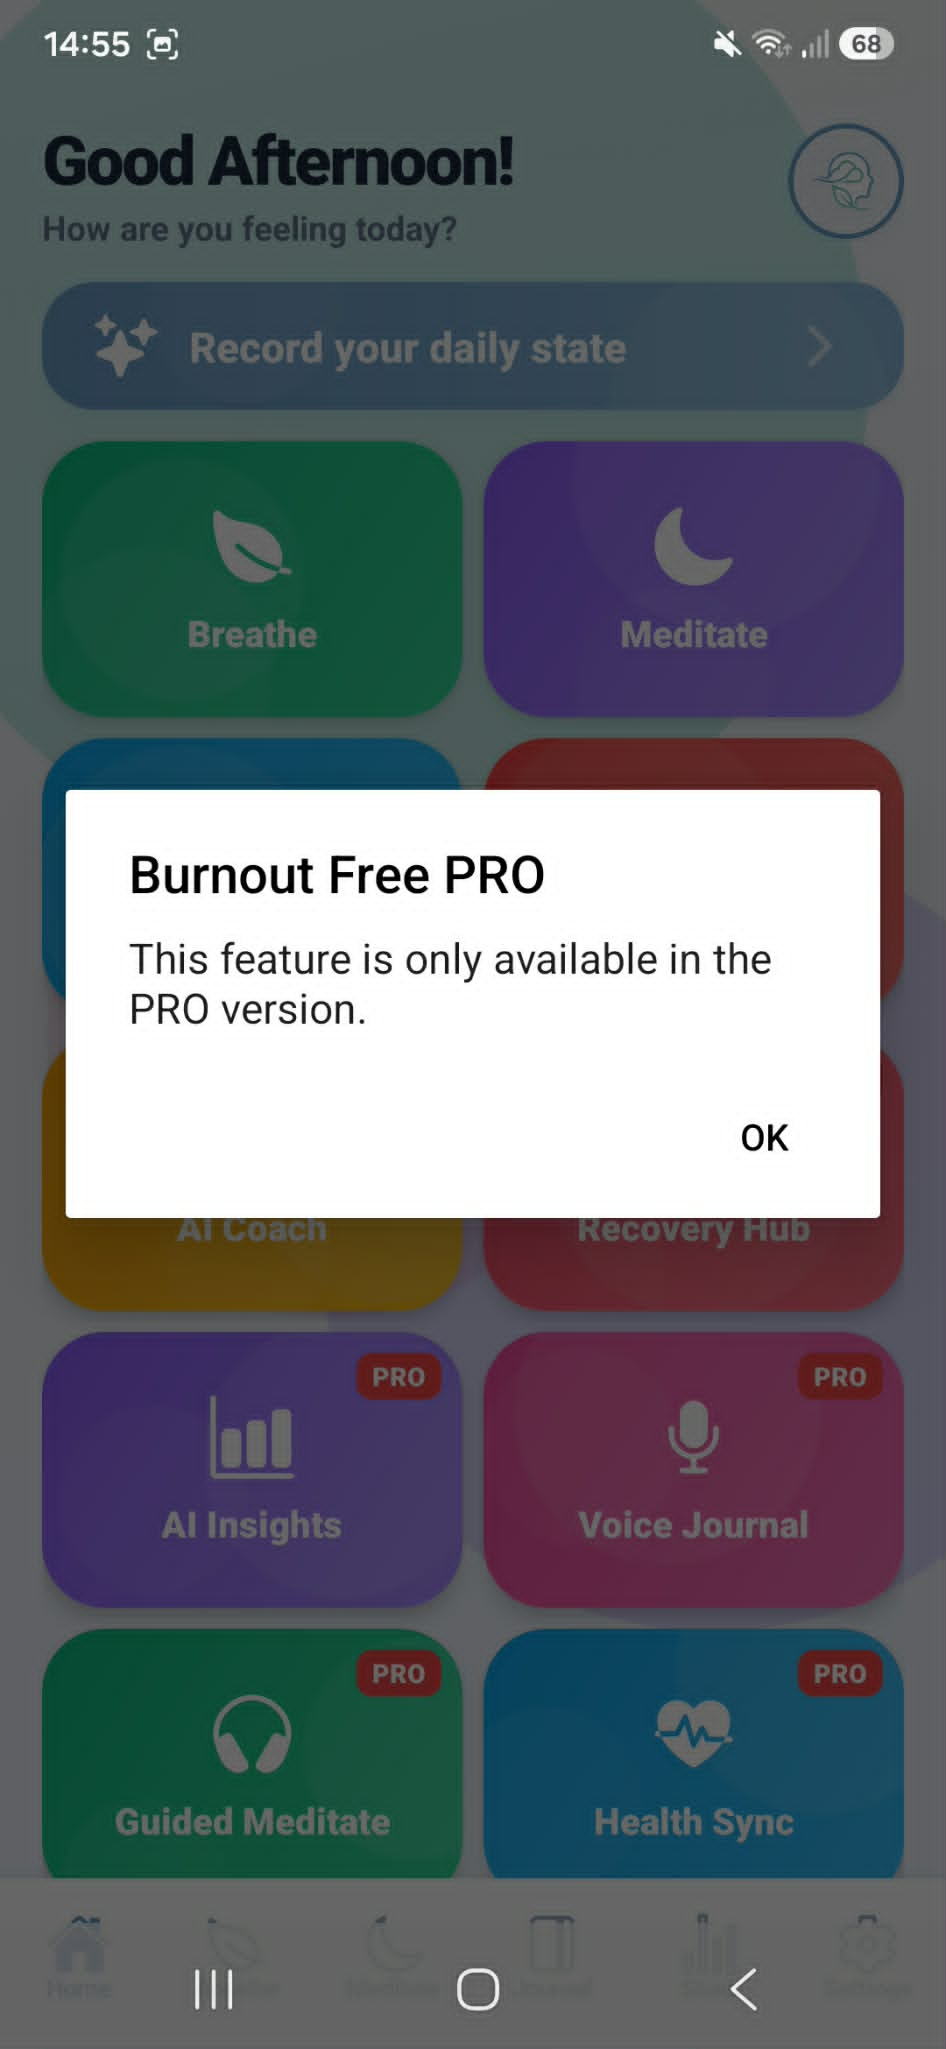
\includegraphics[width=\linewidth]{../graphics/burnoutfree/BurnoutFree13}
    \end{minipage}
    \hfill
    \begin{minipage}{0.3\textwidth}
        \centering
        \phantom{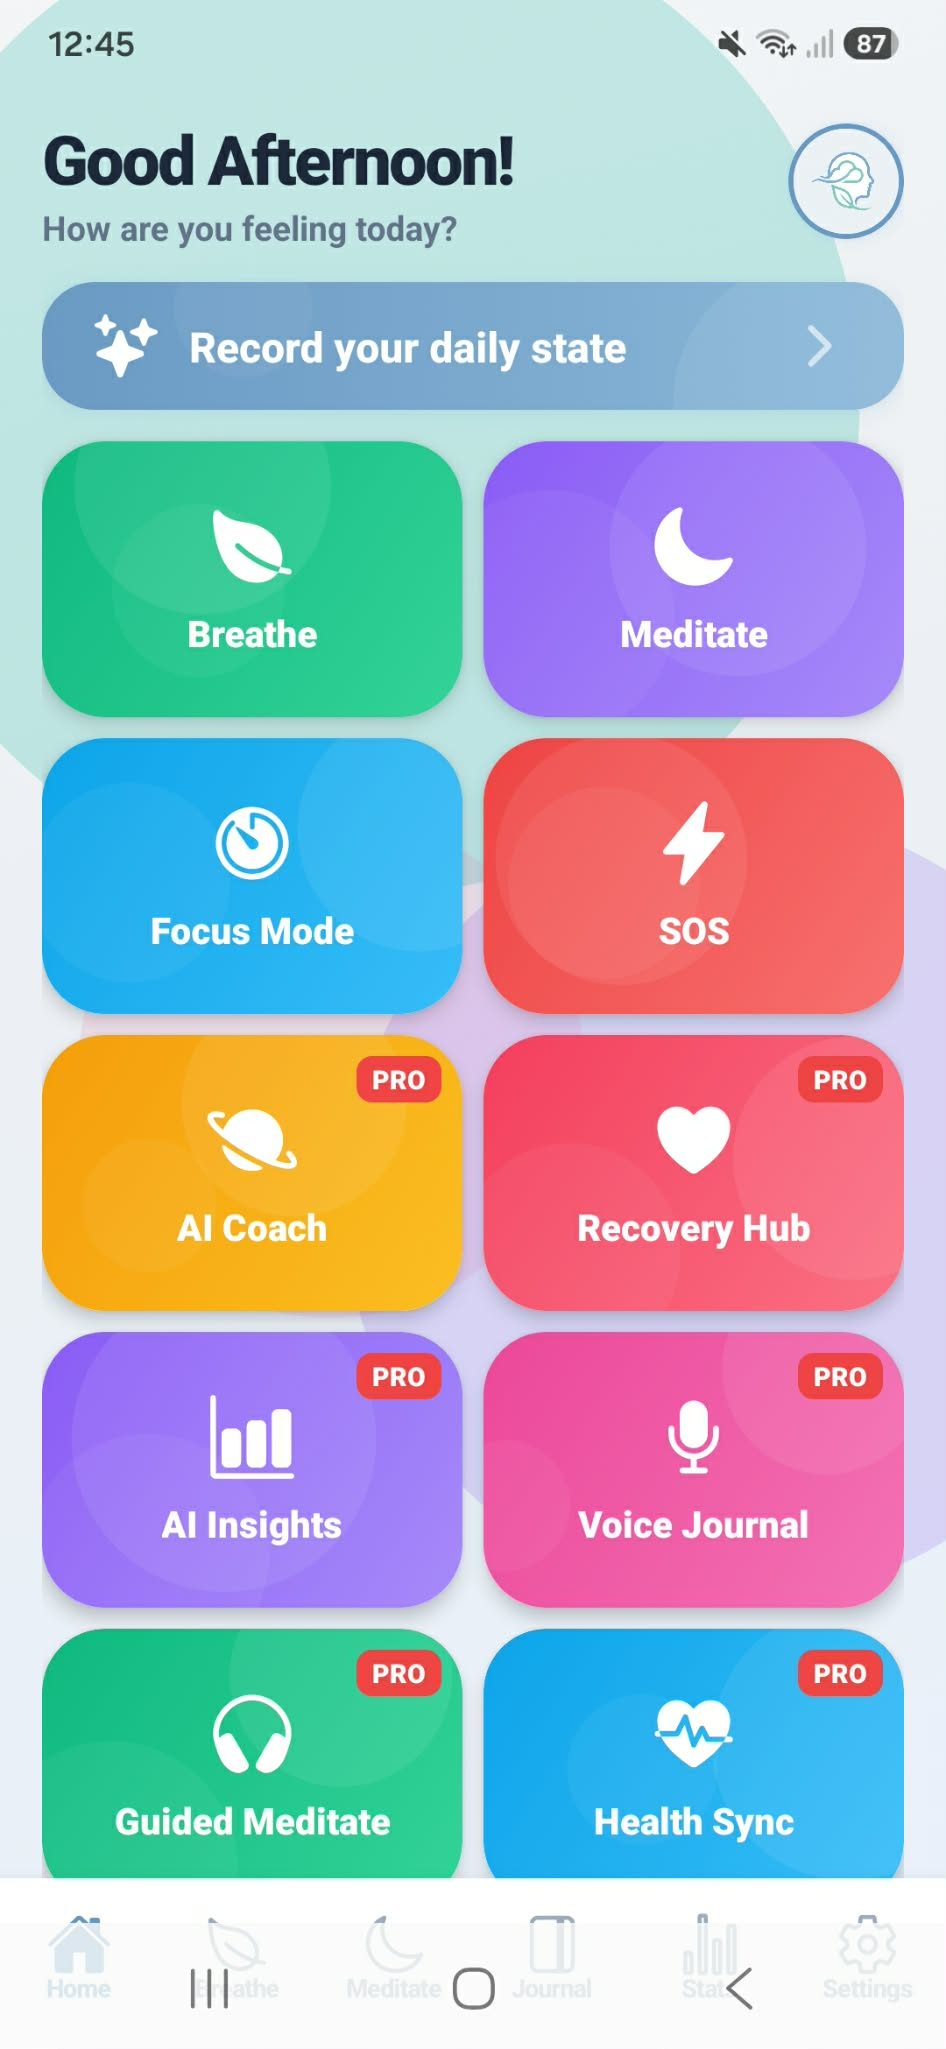
\includegraphics[width=\linewidth]{../graphics/burnoutfree/BurnoutFree1}}
    \end{minipage}
    
    \caption{De instellingenpagina met de foutmelding \texttt{ns\_denied} (links) en de pop-up met informatie over het Burnout Free Pro-plan (midden).}
    \label{fig:burnout-free-6}
\end{figure}

\newpage

\subsection{Aftoetsing functionele requirements}
\label{subsec:frs-burnoutfree}

\vspace{1em}

Onderstaande tabel toont de aftoetsing van de functionele requirements aan de huidige Burnout Free app. Hierbij wordt nagegaan welke functionaliteiten reeds aanwezig zijn en welke ontbreken. Requirements die niet teruggevonden werden in de app worden visueel gemarkeerd met een lichtere grijstint.

\vspace{2em}

{\small
    \textcolor{green!80!black}{\textbf{M}}ust have \quad
    \textcolor{orange}{\textbf{S}}hould have \quad
    \textcolor{blue}{\textbf{C}}ould have \quad
    \textcolor{black!60}{\textbf{W}}on’t have
}

{
    \small
    \setlength\tabcolsep{3pt}
    \begin{longtable}{
            >{\raggedright\arraybackslash}p{3.0cm}
            >{\raggedright\arraybackslash}p{10.5cm}
            >{\centering\arraybackslash}p{2.0cm}
        }
        \toprule
        \textbf{Rol} & \textbf{Functionaliteit} & \textbf{Prioriteit} \\
        \midrule
        \endfirsthead
        
        \multicolumn{3}{c}{\tablename\ \thetable\ -- vervolg van vorige pagina} \\
        \toprule
        \textbf{Rol} & \textbf{Functionaliteit} & \textbf{Prioriteit} \\
        \midrule
        \endhead
        
        \midrule \multicolumn{3}{r}{Vervolg op volgende pagina} \\
        \endfoot
        
        \bottomrule
        \caption[Overzicht requirements]{Oplijsting van functionele requirements met MoSCoW-prioriteit.}
        \label{tab:requirements-burnoutfree}
        \endlastfoot
        \addlinespace[6pt]
        
        %==============================
        \textcolor{gray!40}{Gebruiker} & \textcolor{gray!40}{Registreren en aanmelden} & \textcolor{gray!40}{\textbf{M}} \\
        Alle rollen & Raadplegen privacybeleid en juridische info & \textcolor{green!80!black}{\textbf{M}} \\
        \textcolor{gray!40}{Admin} & \textcolor{gray!40}{Beheren van gebruikers} & \textcolor{gray!40}{\textbf{M}} \\
        \textcolor{gray!40}{Admin} & \textcolor{gray!40}{Modereren van community} & \textcolor{gray!40}{\textbf{M}} \\
        \textcolor{gray!40}{Admin} & \textcolor{gray!40}{Beheren van hulpinstanties} & \textcolor{gray!40}{\textbf{M}} \\
        \textcolor{gray!40}{Expert} & \textcolor{gray!40}{Registreren als expert} & \textcolor{gray!40}{\textbf{M}} \\
        \textcolor{gray!40}{Expert} & \textcolor{gray!40}{Toevoegen van educatieve content} & \textcolor{gray!40}{\textbf{C}} \\
        \textcolor{gray!40}{Expert} & \textcolor{gray!40}{Aanpassen van educatieve content} & \textcolor{gray!40}{\textbf{S}} \\
        \textcolor{gray!40}{Expert} & \textcolor{gray!40}{Valideren van educatieve content} & \textcolor{gray!40}{\textbf{S}} \\ 
        \addlinespace[20pt]
        
        \multicolumn{3}{l}{\textbf{Onboarding \& personalisatie}} \\ \addlinespace[6pt]
        \textcolor{gray!40}{Gebruiker} & \textcolor{gray!40}{Doorlopen van visuele onboarding} & \textcolor{gray!40}{\textbf{M}} \\
        \textcolor{gray!40}{Gebruiker} & \textcolor{gray!40}{Personaliseren van profiel} & \textcolor{gray!40}{\textbf{C}} \\
        \textcolor{gray!40}{Gebruiker} & \textcolor{gray!40}{Personaliseren van dashboard} & \textcolor{gray!40}{\textbf{S}} \\
        \textcolor{gray!40}{Gebruiker} & \textcolor{gray!40}{Instellen van begeleidingsintensiteit} & \textcolor{gray!40}{\textbf{S}} \\
        \textcolor{gray!40}{Gebruiker} & \textcolor{gray!40}{Instellen van persoonlijke doelen} & \textcolor{gray!40}{\textbf{M}} \\
        Gebruiker & Instellen van notificatiefrequentie & \textcolor{green!80!black}{\textbf{M}} \\
        \textcolor{gray!40}{Gebruiker} & \textcolor{gray!40}{Personaliseren van het aanbod aan oefeningen a.d.h.v. vorderingen binnen het persoonlijk traject} & \textcolor{gray!40}{\textbf{S}} \\
        \addlinespace[20pt]
        
        \multicolumn{3}{l}{\textbf{Zelfreflectie \& dagboek}} \\ \addlinespace[6pt]
        Gebruiker & Registreren van stressniveau & \textcolor{green!80!black}{\textbf{M}} \\
        Gebruiker & Bijhouden van gestructureerd dagboek & \textcolor{green!80!black}{\textbf{M}} \\
        \textcolor{gray!40}{Gebruiker} & \textcolor{gray!40}{Raadplegen van dagboekhistoriek} & \textcolor{gray!40}{\textbf{M}} \\
        \textcolor{gray!40}{Gebruiker} & \textcolor{gray!40}{Exporteren van dagboekgegevens} & \textcolor{gray!40}{\textbf{S}} \\
        \textcolor{gray!40}{Gebruiker} & \textcolor{gray!40}{Automatische analyse / samenvatting van gegevens} & \textcolor{gray!40}{\textbf{S}} \\
        \addlinespace[10pt]
        
        \multicolumn{3}{l}{\textbf{Psycho-educatie}} \\ \addlinespace[6pt]
        \textcolor{gray!40}{Gebruiker} & \textcolor{gray!40}{Raadplegen van educatieve content} & \textcolor{gray!40}{\textbf{M}} \\
        \textcolor{gray!40}{Gebruiker} & \textcolor{gray!40}{Ontvangen van contextuele educatieve feedback} & \textcolor{gray!40}{\textbf{S}} \\
        \addlinespace[20pt]
        
        \multicolumn{3}{l}{\textbf{Oefeningen \& stressregulatie}} \\ \addlinespace[6pt]
        Gebruiker & Raadplegen van stressreducerende oefeningen & \textcolor{green!80!black}{\textbf{M}} \\
        Gebruiker & Raadplegen van begeleide rustmomenten & \textcolor{orange}{\textbf{S}} \\ \addlinespace[20pt]
        
        \multicolumn{3}{l}{\textbf{Feedback \& progressie}} \\ \addlinespace[6pt]
        Gebruiker & Raadplegen van een visuele weergave van de huidige trajectvoortgang & \textcolor{green!80!black}{\textbf{M}} \\
        \textcolor{gray!40}{Gebruiker} & \textcolor{gray!40}{Ontvangen van positieve/informatieve feedback} & \textcolor{gray!40}{\textbf{M}} \\
        \textcolor{gray!40}{Gebruiker} & \textcolor{gray!40}{Niet-competitieve beloningen} & \textcolor{gray!40}{\textbf{C}} \\
        \addlinespace[20pt]
        
        \multicolumn{3}{l}{\textbf{Notificaties \& nudging}} \\ \addlinespace[6pt]
        \textcolor{gray!40}{Gebruiker} & \textcolor{gray!40}{Ontvangen van gepersonaliseerde notificaties} & \textcolor{gray!40}{\textbf{S}} \\
        \textcolor{gray!40}{Gebruiker} & \textcolor{gray!40}{Interactieve notificaties} & \textcolor{gray!40}{\textbf{C}} \\
        \textcolor{gray!40}{Gebruiker} & \textcolor{gray!40}{Gedragsgerichte nudges ontvangen} & \textcolor{gray!40}{\textbf{S}} \\ 
        \addlinespace[20pt]
        
        \multicolumn{3}{l}{\textbf{Verbondenheid \& community}} \\ \addlinespace[6pt]
        \textcolor{gray!40}{Gebruiker} & \textcolor{gray!40}{Interageren op een laagdrempelige manier zonder prestatie- of vergelijkingsmechanismen} & \textcolor{gray!40}{\textbf{C}} \\
        \textcolor{gray!40}{Gebruiker} & \textcolor{gray!40}{Versturen/ontvangen van anonieme aanmoedigingen} & \textcolor{gray!40}{\textbf{S}} \\
        \textcolor{gray!40}{Gebruiker} & \textcolor{gray!40}{Controle over zichtbaarheid en gedeelde informatie} & \textcolor{gray!40}{\textbf{M}} \\ \addlinespace[20pt]
        
        \multicolumn{3}{l}{\textbf{Motivatie \& engagement}} \\ \addlinespace[6pt]
        \textcolor{gray!40}{Gebruiker} & \textcolor{gray!40}{Progressiesysteem / verhaallijn} & \textcolor{gray!40}{\textbf{S}} \\ \addlinespace[20pt]
        
        \multicolumn{3}{l}{\textbf{Hulp \& doorverwijzing}} \\ \addlinespace[6pt]
        \textcolor{gray!40}{Gebruiker} & \textcolor{gray!40}{Raadplegen van professionele hulpopties} & \textcolor{gray!40}{\textbf{M}} \\
        \textcolor{gray!40}{Gebruiker} & \textcolor{gray!40}{Ontvangen van advies tot doorverwijzing} & \textcolor{gray!40}{\textbf{M}} \\
        
    \end{longtable}
}

\vspace{1em}

\subsection{Aftoetsing ontwerpprincipes}
\label{subsec:ontwerpprincipes-burnoutfree}

\vspace{1em}

Onderstaande tabel toont de aftoetsing van de ontwerpprincipes aan de huidige Burnout Free app. Per ontwerpprincipe wordt geëvalueerd welke elementen reeds aanwezig zijn en waar nog mogelijke verbeterpunten liggen.

\vspace{1em}

{
    \footnotesize
    \setlength\tabcolsep{3pt}
    
    \begin{longtable}{
            >{\raggedright\arraybackslash}p{5.23cm}
            >{\raggedright\arraybackslash}p{4.93cm}
            >{\raggedright\arraybackslash}p{4.93cm}
        }
        
        \toprule
        \textbf{Ontwerpprincipe}
        & \textbf{Toepassing}
        & \textbf{Aandachtspunten} \\
        \midrule
        \endfirsthead
        
        \toprule
        \textbf{Ontwerpprincipe}
        & \textbf{Toepassing}
        & \textbf{Aandachtspunten} \\
        \midrule
        \endhead
        
        \midrule
        \multicolumn{3}{r}{Vervolg op volgende pagina} \\
        \endfoot
        
        \bottomrule
        \endlastfoot
        
        \addlinespace[10pt]
        
        \textbf{1.} Privacy by Design
        & 
        \begin{itemize}[nosep,leftmargin=*,itemsep=10pt]
            \renewcommand{\labelitemi}{+}
            \item Gegevens worden lokaal op het toestel opgeslagen en worden volgens het privacybeleid niet gedeeld met derde partijen.
            \item De applicatie verzamelt volgens het privacybeleid geen persoonlijke gegevens voor externe verwerking.
        \end{itemize}
        & 
        \begin{itemize}[nosep,leftmargin=*,itemsep=10pt]
            \renewcommand{\labelitemi}{-}
            \item Het privacybeleid is niet onmiddellijk zichtbaar en vereist verdere navigatie naar het instellingenmenu.
            \item Het is onduidelijk hoe gebruikersgegevens verwerkt worden bij het gebruik van AI-functies zoals AI Insights en AI Coach.
        \end{itemize}
        \\
        
        \addlinespace[5pt]
        
        \textbf{2.} Snel en eenvoudig distribueerbaar
        & 
        \begin{itemize}[nosep,leftmargin=*,itemsep=10pt]
            \renewcommand{\labelitemi}{+}
            \item Beschikbaar via de Google Play Store, waardoor gebruikers de applicatie eenvoudig kunnen vinden en installeren.
            \item De applicatie heeft een beperkte bestandsgrootte van 39,11 MB waardoor de download- en installatiedrempel laag blijft.
        \end{itemize}
        & 
        \begin{itemize}[nosep,leftmargin=*,itemsep=10pt]
            \renewcommand{\labelitemi}{-}
            \item De applicatie lijkt enkel beschikbaar via Android, waardoor iOS-gebruikers geen toegang hebben tot dezelfde applicatie.
        \end{itemize}
        \\
        
        \addlinespace[5pt]
        
        \textbf{3.} Ondersteunende foutafhandeling
        & 
        \begin{itemize}[nosep,leftmargin=*,itemsep=10pt]
            \renewcommand{\labelitemi}{+}
            \item De app voorkomt invoerfouten door gebruik te maken van vooraf bepaalde keuzewaarden bij het invullen van een journal. Gebruikers kunnen hierdoor geen ongeldige waarden invoeren.
        \end{itemize}
        & 
        \begin{itemize}[nosep,leftmargin=*,itemsep=10pt]
            \renewcommand{\labelitemi}{-}
            \item Sommige (fout)meldingen zijn technisch geformuleerd en/of bieden onvoldoende uitleg (bv. "ns\_denied").
            \item Ingevoerde noodcontactgegevens worden niet gevalideerd, waardoor ongeldige gegevens opgeslagen kunnen worden.
        \end{itemize}
        \\
        
        \addlinespace[5pt]
        
        \textbf{4.} Inclusieve toegankelijkheid
        & 
        \begin{itemize}[nosep,leftmargin=*,itemsep=10pt]
            \renewcommand{\labelitemi}{+}
            \item De app ondersteunt meerdere talen.
            \item De app ondersteunt dark mode.
            \item De app werkt met een screenreader.
        \end{itemize}
        & 
        \begin{itemize}[nosep,leftmargin=*,itemsep=10pt]
            \renewcommand{\labelitemi}{-}
            \item Bij grotere tekstinstellingen breken sommige menu-items.
            \item Sommige teksten op de statistiekenpagina zijn standaard klein weergegeven en daardoor moeilijker leesbaar.
            \item Het onderste navigatiemenu is moeilijk bereikbaar op bepaalde toestellen doordat het overlapt met de systeemnavigatie van het toestel.
        \end{itemize}
        \\
        
        \addlinespace[5pt]
        
        \textbf{5.} Beperk digitale interrupties
        & 
        \begin{itemize}[nosep,leftmargin=*,itemsep=10pt]
            \renewcommand{\labelitemi}{+}
            \item Gebruikers kunnen zelf kiezen voor welke functionaliteiten zij herinneringen willen ontvangen.
            \item Het tijdstip van herinneringen kan per soort door de gebruiker aangepast worden.
        \end{itemize}
        & 
        \begin{itemize}[nosep,leftmargin=*,itemsep=10pt]
            \renewcommand{\labelitemi}{-}
            \item Er is geen mogelijkheid om de frequentie van herinneringen aan te passen.
        \end{itemize}
        \\
        
        \addlinespace[5pt]
        
        \textbf{6.} Behoud overzicht
        & 
        \begin{itemize}[nosep,leftmargin=*,itemsep=10pt]
            \renewcommand{\labelitemi}{+}
            \item Informatie wordt beperkt weergegeven, waardoor schermen overzichtelijk blijven.
            \item De gebruiker krijgt per pagina een duidelijk beeld van het doel en de beschikbare acties.
        \end{itemize}
        & 
        \begin{itemize}[nosep,leftmargin=*,itemsep=10pt]
            \renewcommand{\labelitemi}{-}
            \item De startpagina bevat veel mogelijke acties, waardoor de primaire keuze minder duidelijk is.
            \item De pro-versie functionaliteiten lijken beschikbaar, maar zijn niet toegankelijk waardoor de startpagina minder overzichtelijk wordt.
            \item Het instellingenicoon is niet onmiddellijk herkenbaar.
            \item De primaire actie voor het starten van een oefening is pas zichtbaar na het scrollen.
        \end{itemize}
        \\
        
        \addlinespace[5pt]
        
        \textbf{7.} Minimaliseer cognitieve belasting
        & 
        \begin{itemize}[nosep,leftmargin=*,itemsep=10pt]
            \renewcommand{\labelitemi}{+}
            \item Schermen bevatten weinig informatie, waardoor de applicatie snel scanbaar is.
            \item Telkens één duidelijke taak per scherm.
        \end{itemize}
        & 
        \begin{itemize}[nosep,leftmargin=*,itemsep=10pt]
            \renewcommand{\labelitemi}{-}
            \item Er wordt echter weinig tot geen uitleg of psycho- educatie aangeboden, waardoor gebruikers soms onvoldoende begrijpen waarom een oefening nuttig is. Het waarborgen van minimale cognitieve belasting gaat in dit voorbeeld dus ten koste van het aantonen van de therapeutische meerwaarde.
        \end{itemize}
        \\
        
        \addlinespace[5pt]
        
        \textbf{8.} Vermijd visuele overprikkeling
        & 
        \begin{itemize}[nosep,leftmargin=*,itemsep=10pt]
            \renewcommand{\labelitemi}{+}
            \item Er wordt gebruik gemaakt van zachte kleuren die afzonderlijk een rustgevende uitstraling hebben.
            \item De applicatie gebruikt één consistent lettertype.
            \item Animaties binnen ademhalingsoefeningen ondersteunen de functionaliteit en dragen bij aan de gebruikerservaring.
        \end{itemize}
        & 
        \begin{itemize}[nosep,leftmargin=*,itemsep=10pt]
            \renewcommand{\labelitemi}{-}
            \item Er worden, op bijvoorbeeld de homepagina, veel verschillende (en fellere) kleuren gecombineerd.
            \item Decoratieve animaties op de achtergrond en binnen knoppen voegen weinig functionele meerwaarde toe en kunnen onnodige afleiding veroorzaken.
            \item Inconsistente overgangs- animaties (naar links, naar rechts of zonder animatie)
        \end{itemize}
        \\
        
        \addlinespace[5pt]
        
        \textbf{9.} Techno-simplicity
        & 
        \begin{itemize}[nosep,leftmargin=*,itemsep=10pt]
            \renewcommand{\labelitemi}{+}
            \item De applicatie heeft een eenvoudige structuur waardoor gebruikers snel zelfstandig hun weg vinden.
        \end{itemize}
        & 
        \begin{itemize}[nosep,leftmargin=*,itemsep=10pt]
            \renewcommand{\labelitemi}{-}
            \item Er wordt geen onboarding voorzien, waardoor nieuwe gebruikers zonder introductie starten.
            \item Er wordt weinig context gegeven over het doel en de meerwaarde van oefeningen.
        \end{itemize}
        \\
        
        \addlinespace[5pt]
        
        \textbf{10.} Stimuleer gezond gebruik
        & 
        \begin{itemize}[nosep,leftmargin=*,itemsep=10pt]
            \renewcommand{\labelitemi}{+}
            \item Notificaties zijn beperkt tot maximum één per dag per functionaliteit.
        \end{itemize}
        & 
        \begin{itemize}[nosep,leftmargin=*,itemsep=10pt]
            \renewcommand{\labelitemi}{-}
            \item De applicatie gebruikt verschillende streak- systemen (zoals aantal opeenvolgende dagen, minuten oefenen en sessies), wat terugkeer kan stimuleren vanuit prestatiedruk.
        \end{itemize}
        \\
        
        \addlinespace[5pt]
        
        \textbf{11.} Zachte gedragssturing
        & 
        \begin{itemize}[nosep,leftmargin=*,itemsep=10pt]
            \renewcommand{\labelitemi}{+}
            \item Gebruikers kunnen zelf bepalen welke herinneringen zij ontvangen en op welk tijdstip deze verschijnen.
        \end{itemize}
        & 
        \begin{itemize}[nosep,leftmargin=*,itemsep=10pt]
            \renewcommand{\labelitemi}{-}
            \item Herinneringen worden niet aangepast op basis van gebruikerscontext of gebruikspatronen.
            \item Er worden geen gepersonaliseerde suggesties aangeboden op basis van ingevulde journalgegevens.
            \item De gebruiker krijgt weinig begeleiding bij het kiezen van een geschikte oefening.
        \end{itemize}
        \\
        
        \addlinespace[5pt]
        
        \textbf{12.} Ondersteun autonomie
        & 
        \begin{itemize}[nosep,leftmargin=*,itemsep=10pt]
            \renewcommand{\labelitemi}{+}
            \item Gebruikers kunnen zelf kiezen welke oefeningen zij uitvoeren.
            \item Basisvoorkeuren zoals soorten notificaties, taal en een noodcontact zijn instelbaar.
        \end{itemize}
        & 
        \begin{itemize}[nosep,leftmargin=*,itemsep=10pt]
            \renewcommand{\labelitemi}{-}
            \item Gebruikers krijgen onvoldoende ondersteuning bij het kiezen van de meest geschikte oefening.
            \item Geen personalisatie- mogelijkheden buiten de basisinstellingen.
            \item Sommige formuleringen zijn minder uitnodigend (bv. \textit{"Track your progress"}, \textit{"Find your peace and focus"}).
        \end{itemize}
        \\
        
        \addlinespace[5pt]
        
        \textbf{13.} Ondersteun competentiegevoel
        & 
        \begin{itemize}[nosep,leftmargin=*,itemsep=10pt]
            \renewcommand{\labelitemi}{+}
            \item Acties zijn eenvoudig en laagdrempelig opgebouwd.
            \item Bij ademhalingsoefeningen wordt uitgelegd waarvoor de oefening bedoeld is.
        \end{itemize}
        & 
        \begin{itemize}[nosep,leftmargin=*,itemsep=10pt]
            \renewcommand{\labelitemi}{-}
            \item Gebruikers krijgen geen feedback over het effect van hun ingevulde journal of uitgevoerde oefeningen.
            \item Het is niet altijd duidelijk hoe oefeningen correct uitgevoerd moeten worden of wanneer een bepaalde oefening het meest geschikt is.
            \item De weergegeven voortgang focust voornamelijk op gebruik (sessies, minuten, streaks) en minder op persoonlijk welzijn of ontwikkeling.
        \end{itemize}
        \\
        
        \addlinespace[5pt]
        
        \textbf{14.} Stimuleer authentieke verbondenheid
        & 
        \begin{itemize}[nosep,leftmargin=*,itemsep=10pt]
            \renewcommand{\labelitemi}{+}
            \item Gebruikers kunnen een persoonlijk noodcontact instellen om snel contact op te nemen met iemand uit hun omgeving.
        \end{itemize}
        & 
        \begin{itemize}[nosep,leftmargin=*,itemsep=10pt]
            \renewcommand{\labelitemi}{-}
            \item De app bevat geen component welke directe toegang voorziet tot professionele hulp of peer support.
            \item Geen mogelijkheid om ervaringen te delen of steun te zoeken bij lotgenoten.
        \end{itemize}
        \\
        
        \addlinespace[5pt]
        
        \textbf{15.} Betekenisvolle, prestatievrije motivatie
        &
        & 
        \begin{itemize}[nosep,leftmargin=*,itemsep=10pt]
            \renewcommand{\labelitemi}{-}
            \item De applicatie maakt gebruik van een streak-systeem, wat prestatiedruk kan creëren.
            \item De statistieken focussen voornamelijk op aantallen (sessies, minuten, streaks) en minder op persoonlijke groei of welzijn.
            \item Er worden weinig beloningen of positieve feedback gekoppeld aan het voltooien van oefeningen.
            \item De voortgang wordt niet geëvalueerd of bijgestuurd op basis van de evolutie van de gebruiker.
        \end{itemize}
        \\
        
        \addlinespace[5pt]
        
        \textbf{16.} Persoonlijke relevantie
        &
        & 
        \begin{itemize}[nosep,leftmargin=*,itemsep=10pt]
            \renewcommand{\labelitemi}{-}
            \item Alle beschikbare inhoud is generiek en wordt niet aangepast aan de behoeften of context van de gebruiker.
            \item Journalgegevens worden niet gebruikt om relevante oefeningen of aanbevelingen voor te stellen.
        \end{itemize}
        \\
        
        \addlinespace[5pt]
        
        \textbf{17.} Zichtbare meerwaarde
        &
        & 
        \begin{itemize}[nosep,leftmargin=*,itemsep=10pt]
            \renewcommand{\labelitemi}{-}
            \item Er wordt geen onboarding voorzien waarin het doel en de meerwaarde van de applicatie worden uitgelegd.
            \item De gebruiker krijgt weinig context over waarom bepaalde oefeningen of functionaliteiten nuttig zijn.
            \item Het nut van de journalfunctionaliteit blijft onduidelijk doordat ingevulde gegevens weinig zichtbaar worden gebruikt of teruggekoppeld.
        \end{itemize}
        \\
        
        \addlinespace[5pt]
        
        \textbf{18.} Duidelijke positionering
        & 
        \begin{itemize}[nosep,leftmargin=*,itemsep=10pt]
            \renewcommand{\labelitemi}{+}
            \item De applicatie beschrijft duidelijk dat deze gericht is op mentaal welzijn, stressmanagement en het herkennen van burn-outsignalen.
            \item De belangrijkste functionaliteiten worden concreet benoemd, zoals journaling, meditaties, ademhalingsoefeningen en een focustimer.
            \item De doelgroep wordt expliciet beschreven als professionals, studenten en personen die zich overweldigd voelen.
        \end{itemize}
        & 
        \begin{itemize}[nosep,leftmargin=*,itemsep=10pt]
            \renewcommand{\labelitemi}{-}
            \item Sommige formuleringen kunnen als te sterke beloftes worden geïnterpreteerd, zoals het "\textit{herkennen van burn-outsignalen voordat ze zich voordoen}" en het "\textit{terugkrijgen van controle over mentale gezondheid}". Hoewel de applicatie ondersteuning biedt via tracking en oefeningen, wordt onvoldoende toegelicht hoe deze functionaliteiten bijdragen aan het herkennen of voorkomen van burn-out, waardoor de verwachtingen van gebruikers mogelijk te hoog kunnen liggen.
            \item Er wordt niet expliciet vermeld dat de applicatie geen vervanging is voor professionele hulp.
        \end{itemize}
        \\
        
        \addlinespace[5pt]
        
        \textbf{19.} Ondersteunende communicatie
        & 
        \begin{itemize}[nosep,leftmargin=*,itemsep=10pt]
            \renewcommand{\labelitemi}{+}
            \item De applicatie gebruikt overwegend neutrale en begrijpelijke taal.
        \end{itemize}
        & 
        \begin{itemize}[nosep,leftmargin=*,itemsep=10pt]
            \renewcommand{\labelitemi}{-}
            \item De communicatie is voornamelijk functioneel en biedt weinig empathische terugkoppeling op basis van de situatie van de gebruiker.
        \end{itemize}
        \\ 
    \end{longtable}
}

\newpage

\section{Uitwerking van mockups}
\label{sec:uitwerking-mockups}

\subsection{Startpagina en toolkit}
\label{subsec:startpagina-mockups}

\begin{figure}[H]
    \centering
    
    \begin{minipage}{0.3\textwidth}
        \centering
        
\includegraphics[width=\linewidth]{../graphics/Mockups/Home/Splashscreen}
    \end{minipage}
    \hfill
    \begin{minipage}{0.3\textwidth}
        \centering
        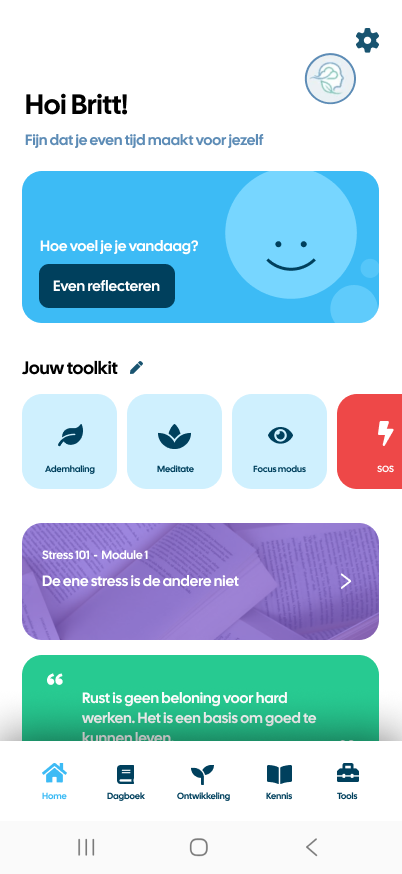
\includegraphics[width=\linewidth]{../graphics/Mockups/Home/Home}
    \end{minipage}
    \hfill
    \begin{minipage}{0.3\textwidth}
        \centering
        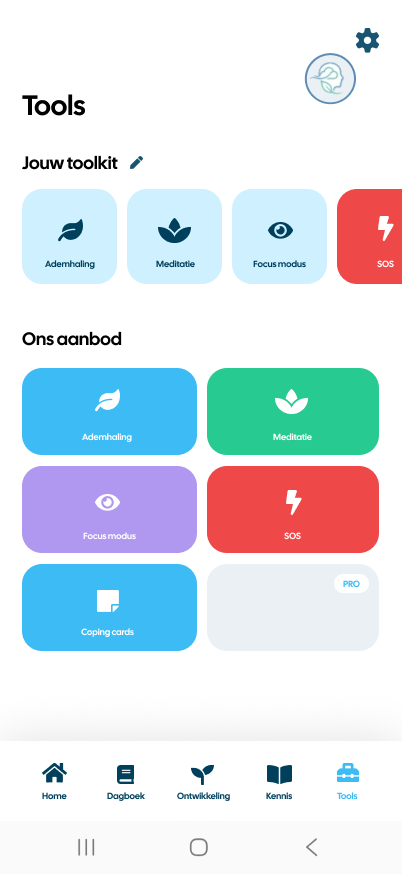
\includegraphics[width=\linewidth]{../graphics/Mockups/Home/Tools}
    \end{minipage}
    
    \caption{Mockups van de splashscreen, startpagina en toolkit}
    \label{fig:mockups-1}
\end{figure}

De voornaamste aandachtspunten in de vorige versie van de applicatie (\ref{fig:burnout-free-1}) waren de overmatige animaties, de beperkte persoonlijke relevantie en het grote gebruik van verschillende kleuren. De beschikbare tools werden voornamelijk algemeen weergegeven, zonder afstemming op de individuele gebruiker. Daarnaast zorgden de decoratieve animaties en de veelheid aan kleuren voor een visueel drukke en mogelijk overprikkelende interface. In de nieuwe versie werd daarom bewust gekozen voor een rustigere, meer persoonlijke en gestructureerde opbouw.

{\small
    \begin{itemize}
        \item De splashscreen bevat een korte ademhalingsoefening, waarbij animatie functioneel wordt ingezet (\textbf{Ontwerpprincipe}: \textit{vermijd visuele overprikkeling}).
        
        \item De hoofdpagina focust op persoonlijk relevante content en tools (\textbf{Ontwerpprincipes}: \textit{persoonlijke relevantie} en \textit{ondersteun autonomie}).
        
        \item De beschikbare tools werden ondergebracht op een aparte toolkitpagina, waardoor nieuwe tools in de toekomst eenvoudig kunnen worden toegevoegd zonder de hoofdpagina te overladen (\textbf{Ontwerpprincipes}: \textit{minimaliseer cognitieve belasting, behoud overzicht}).
        
        \item Het kleurgebruik werd beperkt tot blauw, groen, paars en beperkte "noodkleur" rood (\textbf{Ontwerpprincipe}: \textit{vermijd visuele overprikkeling}).
    \end{itemize}
}


\subsection{Profiel}
\label{subsec:profiel-mockups}

\begin{figure}[H]
    \centering
    
    \begin{minipage}{0.3\textwidth}
        \centering
        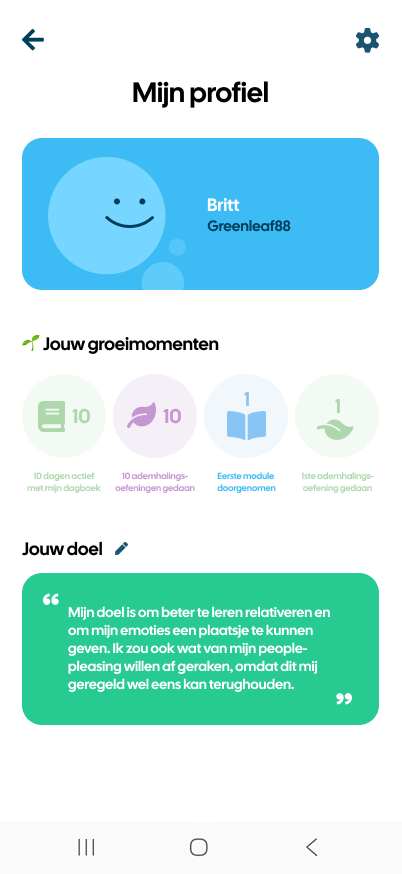
\includegraphics[width=\linewidth]{../graphics/Mockups/Profiel/Profiel1}
    \end{minipage}
    \hfill
    \begin{minipage}{0.3\textwidth}
        \centering
        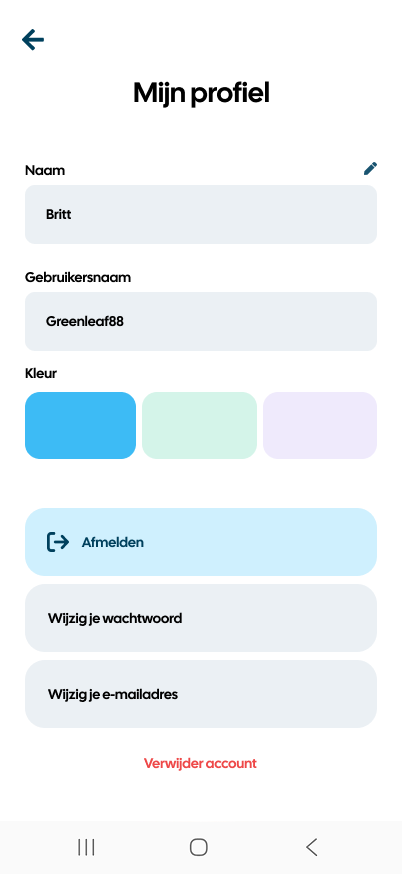
\includegraphics[width=\linewidth]{../graphics/Mockups/Profiel/Profiel2}
    \end{minipage}
    \hfill
    \begin{minipage}{0.3\textwidth}
        \centering
        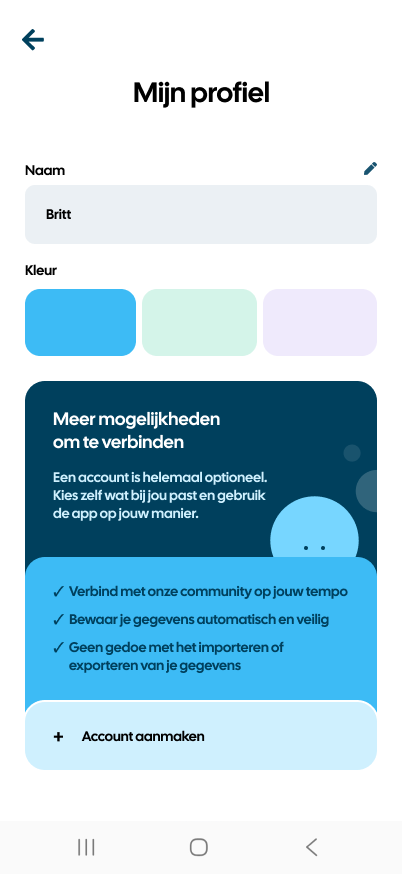
\includegraphics[width=\linewidth]{../graphics/Mockups/Profiel/Profiel3}
    \end{minipage}
    
    \caption{Mockups van het profiel, zowel ingelogd (midden) als niet ingelogd (rechts)}
    \label{fig:mockups-2}
\end{figure}

In de vorige versie van de applicatie was er geen mogelijkheid om een persoonlijk profiel aan te maken. Daarnaast bevatte de applicatie een aparte \textit{statistics}-pagina (\ref{fig:burnout-free-4}) met verschillende prestatiegerichte statistieken, zoals een \textit{daily streak}, het aantal minuten, sessies en dagen waarop de app werd gebruikt. Hierdoor lag de nadruk sterk op het behouden en verhogen van gebruik, wat druk of schuldgevoel kan veroorzaken wanneer een reeks wordt doorbroken. In de nieuwe versie werd daarom gekozen voor een persoonlijk profiel met meer nadruk op persoonlijke doelen en laagdrempelige vooruitgang.

{\small
    \begin{itemize}
        \item De gebruiker kan een eigen naam instellen (\textbf{Ontwerpprincipes}: \textit{persoonlijke relevantie}).
        
        \item De gebruiker kan een persoonlijk doel instellen om bewust te blijven van waarnaar hij of zij streeft (\textbf{Ontwerpprincipes}: \textit{zichtbare meerwaarde, betekenisvolle, prestatievrije motivatie}).
        
        \item Een profiel kan worden aangemaakt zonder dat een account verplicht is, wat de gebruiksdrempel verlaagt (\textbf{Ontwerpprincipe}: \textit{ondersteun autonomie}).
        
        \item De oorspronkelijke prestatiestatistieken werden vervangen door \textit{Jouw groeimomenten}. Deze laagdrempelige badges leggen de nadruk op persoonlijke vooruitgang en kleine successen, zonder gebruiksreeksen of prestatiedoelen te benadrukken (\textbf{Ontwerp- principes}: \textit{stimuleer gezond gebruik, betekenisvolle, prestatievrije motivatie}).
    \end{itemize}
}


\subsection{Instellingen}
\label{subsec:settings-mockups}

\begin{figure}[H]
    \centering
    
    % Linker afbeelding: neemt twee rijen in
    \begin{minipage}{0.3\textwidth}
        \centering
        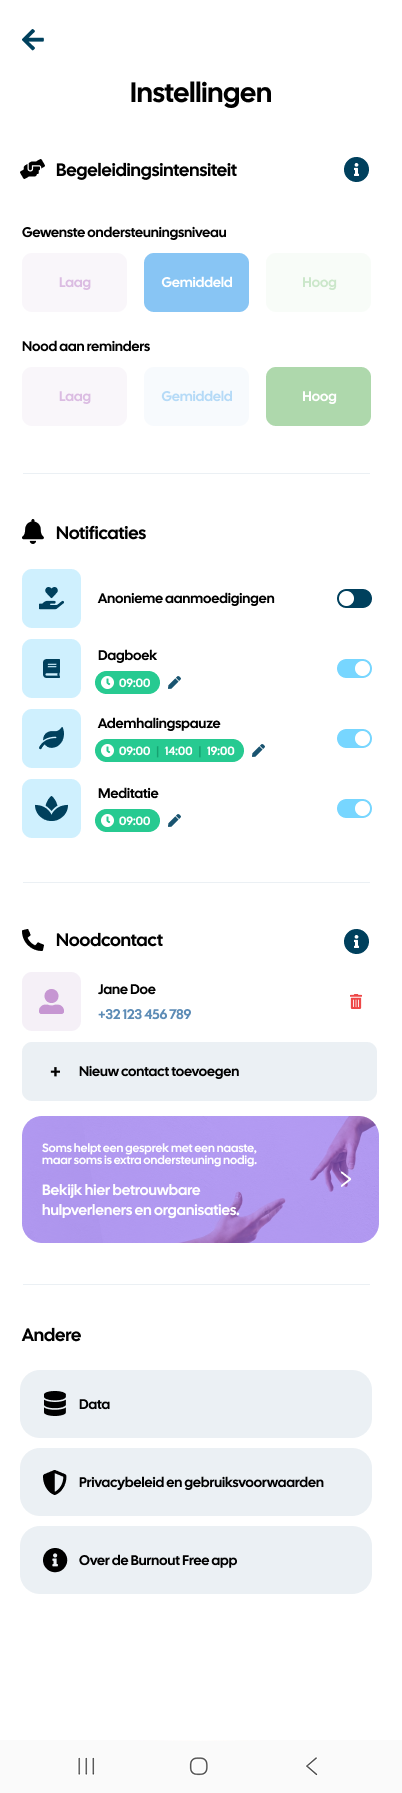
\includegraphics[width=\linewidth]{../graphics/Mockups/Settings/Settings}
    \end{minipage}
    \hfill
    % Rechterkant: 2x2
    \begin{minipage}{0.63\textwidth}
        \centering
        
        % Bovenste rij
        \begin{minipage}{0.47\textwidth}
            \centering
            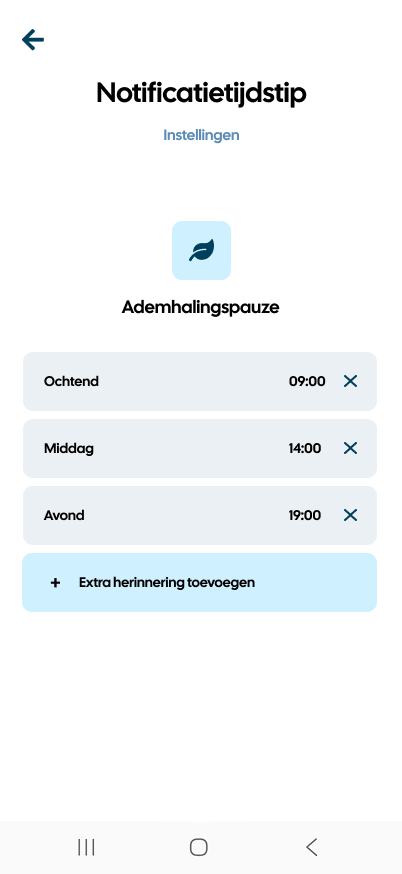
\includegraphics[width=\linewidth]{../graphics/Mockups/Settings/Settings_notificaties}
        \end{minipage}
        \hfill
        \begin{minipage}{0.47\textwidth}
            \centering
            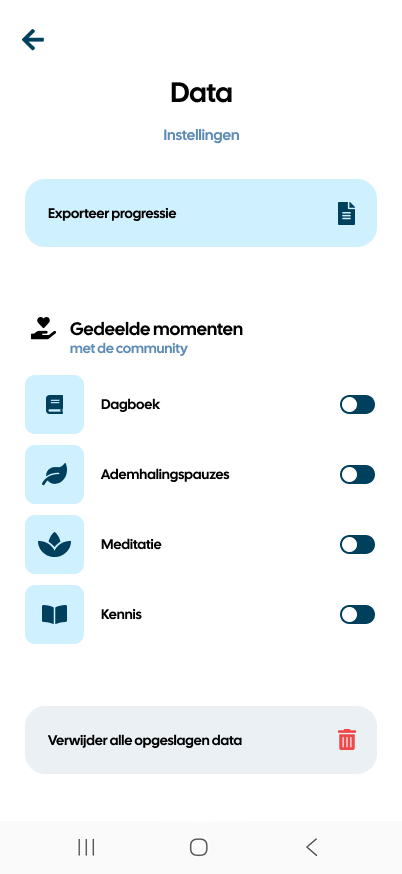
\includegraphics[width=\linewidth]{../graphics/Mockups/Settings/Settings_data_ingelogd}
        \end{minipage}
        
        \vspace{1em}
        
        % Onderste rij
        \begin{minipage}{0.47\textwidth}
            \centering
            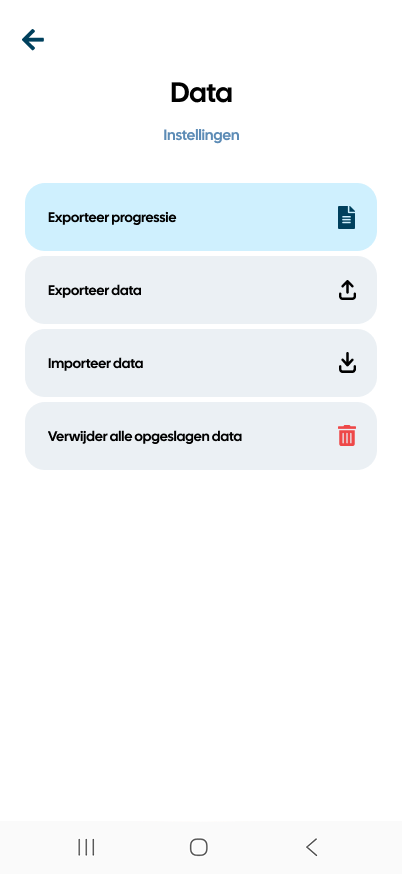
\includegraphics[width=\linewidth]{../graphics/Mockups/Settings/Settings_data}
        \end{minipage}
        \hfill
        \begin{minipage}{0.47\textwidth}
            \centering
            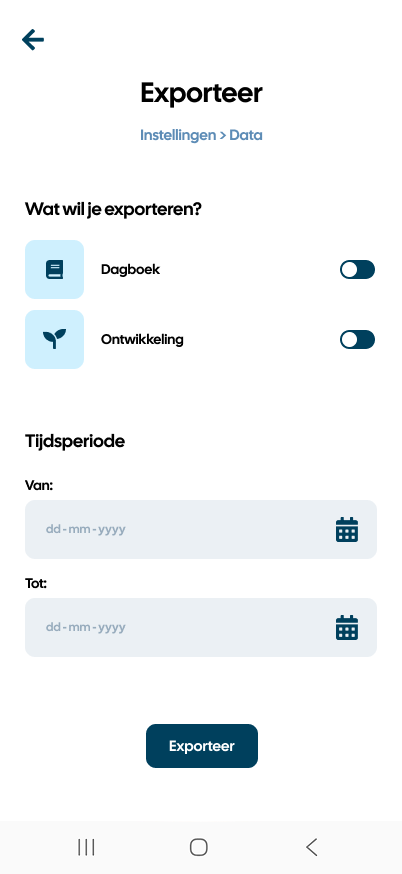
\includegraphics[width=\linewidth]{../graphics/Mockups/Settings/Settings_export}
        \end{minipage}
    \end{minipage}
    
    \caption{Mockups van de instellingen}
    \label{fig:mockups-3}
\end{figure}

In de vorige versie (\ref{fig:burnout-free-4}) waren de instellingen voornamelijk gericht op notificaties, een noodcontact, taal en algemene informatie over de applicatie. De notificaties waren al instelbaar per functionaliteit en tijdstip, maar konden nog beter worden afgestemd op de individuele behoeften van de gebruiker. Daarnaast was er slechts één noodcontact mogelijk en werd de systeemtaal opnieuw uitgevraagd. In de nieuwe versie ligt de focus meer op persoonlijke controle, aangepaste begeleiding en transparant databeheer.

\vspace{1em}

{\small
    \begin{itemize}
        \item De notificatie-instellingen werden uitgebreid met een instelbare begeleidingsintensiteit. Op basis hiervan worden een geschikte hoeveelheid notificaties en aanbevolen tijdstippen voorgesteld, die de gebruiker steeds kan aanpassen (\textbf{Ontwerpprincipes}: \textit{beperk digitale interrupties, zachte gedragssturing, ondersteun autonomie}).
        
        \item De gebruiker kan meerdere noodcontacten toevoegen in plaats van slechts één. Hierdoor kan de gebruiker verschillende personen aanduiden, zoals een vriend, familielid of hulpverlener, zonder verplicht te zijn een contact toe te voegen (\textbf{Ontwerpprincipe}: \textit{stimuleer authentieke verbondenheid, ondersteun autonomie}).
        
        \item De instelling voor systeemtaal werd verwijderd, aangezien de taal automatisch vanuit de systeeminstellingen kan worden bepaald. Hierdoor wordt een overbodige keuze voor de gebruiker vermeden (\textbf{Ontwerpprincipe}: \textit{minimaliseer cognitieve belasting}).
        
        \item Een aparte data-instelling geeft de gebruiker meer controle over de opslag en het gebruik van persoonlijke gegevens (\textbf{Ontwerpprincipes}: \textit{Privacy by Design, ondersteun autonomie}).
        
        \item Gebruikers zonder account kunnen hun lokale gegevens exporteren en importeren om zelf back-ups te beheren (\textbf{Ontwerpprincipes}: \textit{Privacy by Design, ondersteun autonomie}).
        
        \item Ingelogde gebruikers kunnen per functionaliteit bepalen of hun vooruitgang gedeeld mag worden binnen de community. Hierdoor behoudt de gebruiker controle over welke persoonlijke informatie wordt gedeeld (\textbf{Ontwerpprincipes}: \textit{Privacy by Design, stimuleer authentieke verbondenheid, ondersteun autonomie}).
        
        \item Via de exportfunctie kan de gebruiker een selectie van zijn of haar voortgang exporteren voor eigen analyse of om deze bijvoorbeeld te bespreken met een psycholoog (\textbf{Ontwerpprincipes}: \textit{zichtbare meerwaarde, ondersteun autonomie}).
    \end{itemize}
}

\vspace{1em}
\vspace{1em}


\subsection{Oefeningen}
\label{subsec:oefeningen-mockups}

\vspace{1em}

\subsubsection{Meditatie}
\label{subsubsec:meditatie-mockups}

\begin{figure}[H]
    \centering
    
    \begin{minipage}{0.3\textwidth}
        \centering
        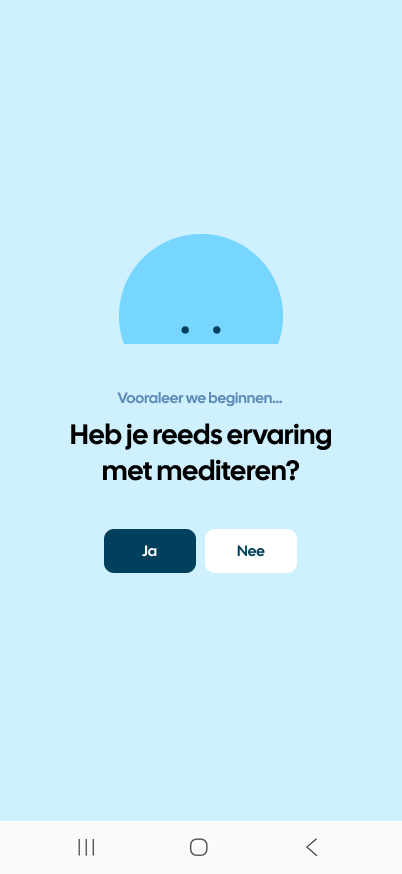
\includegraphics[width=\linewidth]{../graphics/Mockups/Oefeningen/meditatie/Meditatie_tutorial1}
    \end{minipage}
    \hfill
    \begin{minipage}{0.3\textwidth}
        \centering
        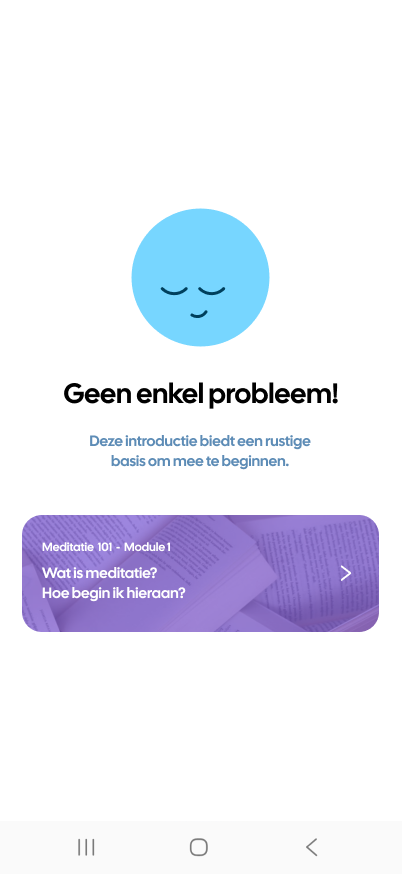
\includegraphics[width=\linewidth]{../graphics/Mockups/Oefeningen/meditatie/Meditatie_tutorial2}
    \end{minipage}
    \hfill
    \begin{minipage}{0.3\textwidth}
        \centering
        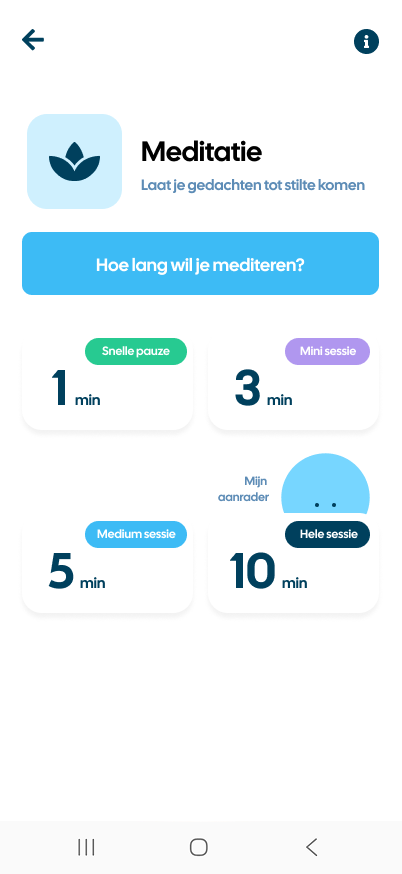
\includegraphics[width=\linewidth]{../graphics/Mockups/Oefeningen/meditatie/Meditatie1}
    \end{minipage}
    
    \vspace{1em}
    
    \begin{minipage}{0.3\textwidth}
        \centering
        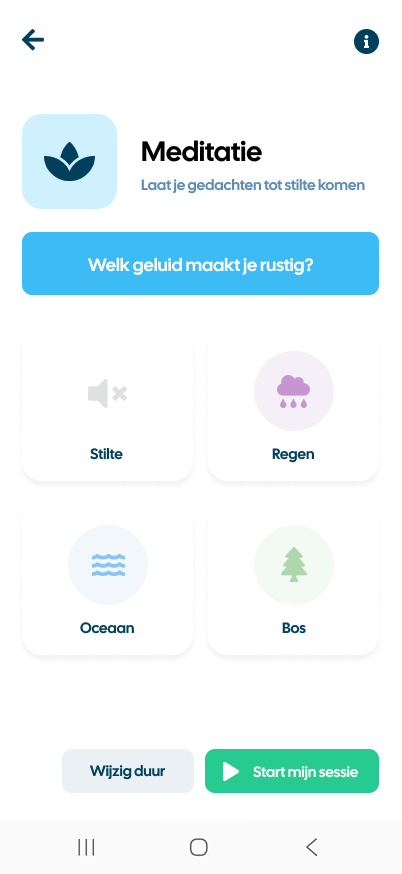
\includegraphics[width=\linewidth]{../graphics/Mockups/Oefeningen/meditatie/Meditatie2}
    \end{minipage}
    \hfill
    \begin{minipage}{0.3\textwidth}
        \centering
        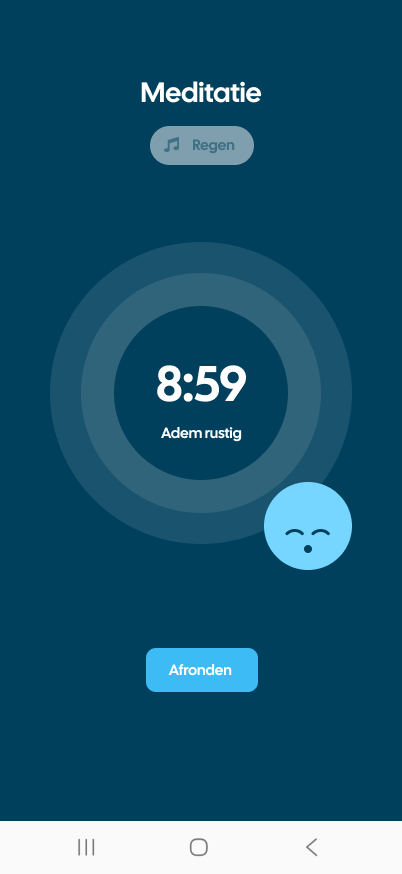
\includegraphics[width=\linewidth]{../graphics/Mockups/Oefeningen/meditatie/Meditatie3}
    \end{minipage}
    \hfill
    \begin{minipage}{0.3\textwidth}
        \centering
        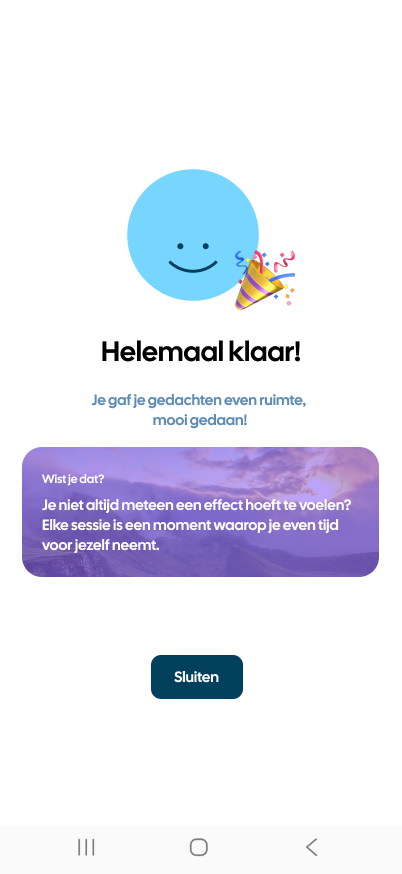
\includegraphics[width=\linewidth]{../graphics/Mockups/Oefeningen/meditatie/Meditatie4}
    \end{minipage}
    
    \caption{Mockups van meditatie oefeningen}
    \label{fig:mockups-4}
\end{figure}

In de vorige versie van de meditatie-oefening (\ref{fig:burnout-free-3}) werd veel informatie tegelijk aangeboden. Zo werden de duur en het geluid op één scherm gekozen en werden keuzes achteraf opnieuw weergegeven. Ook het meditatiescherm bevatte zowel een timer als een progressiebalk met dezelfde informatie, naast verschillende bewegende cirkels op de achtergrond. Na afloop ontbrak bovendien feedback over het voltooien van de oefening. In de nieuwe versie werd daarom gekozen voor een meer stapsgewijze ervaring.

\vspace{1em}

{\small
    \begin{itemize}
        \item Voor de eerste meditatiesessie binnen de app wordt nagegaan of de gebruiker al ervaring heeft met mediteren. Gebruikers zonder ervaring krijgen indien nodig een relevante cursus aangeboden (\textbf{Ontwerpprincipe}: \textit{ondersteun competentiegevoel}).
        
        \item De keuze van de meditatieduur en het geluid werd opgesplitst over afzonderlijke schermen, waardoor informatie stapsgewijs wordt aangeboden (\textbf{Ontwerpprincipes}: \textit{minimaliseer cognitieve belasting, behoud overzicht}).
        
        \item Op basis van de ingestelde begeleidingsintensiteit wordt een passende meditatieduur aanbevolen (\textbf{Ontwerpprincipes}: \textit{persoonlijke relevantie, zachte gedragssturing}).
        
        \item Het meditatiescherm werd vereenvoudigd tot een timer en een functionele ademhalingsanimatie. Overbodige elementen werden verwijderd (\textbf{Ontwerpprincipe}: \textit{vermijd visuele overprikkeling}).
        
        \item Een digitale coach begeleidt de gebruiker tijdens de oefening en ademt mee. Dit biedt ondersteuning zonder prestatiedruk en maakt gebruik van een narratief element (\textbf{Ontwerpprincipe}: \textit{betekenisvolle, prestatievrije motivatie}).
        
        \item Na afloop krijgt de gebruiker feedback over de voltooide oefening en wordt kort toegelicht wat werd bereikt. Een \textit{wist-je-datje} biedt hierbij aanvullende, relevante informatie (\textbf{Ontwerpprincipes}: \textit{ondersteun competentiegevoel, zichtbare meerwaarde}).
    \end{itemize}
}

\vspace{1em}
\vspace{1em}

\subsubsection{Ademhalingsoefeningen}
\label{subsubsec:ademhaling-mockups}

\vspace{1em}

In de vorige versie (\ref{fig:burnout-free-2}) werden verschillende ademhalingsoefeningen aangeboden op basis van hun naam. De kaarten bevatten hierbij relatief veel informatie, waaronder het type oefening en de exacte verdeling van de ademhaling. Ook tijdens de oefening waren naast de functionele ademhalingsanimatie verschillende bewegende elementen aanwezig, wat voor onnodige visuele prikkels zorgde. In de nieuwe versie werd de keuze meer afgestemd op de behoefte van de gebruiker en werd de oefening zelf vereenvoudigd.

\begin{figure}[H]
    \centering
    
    \begin{minipage}{0.3\textwidth}
        \centering
        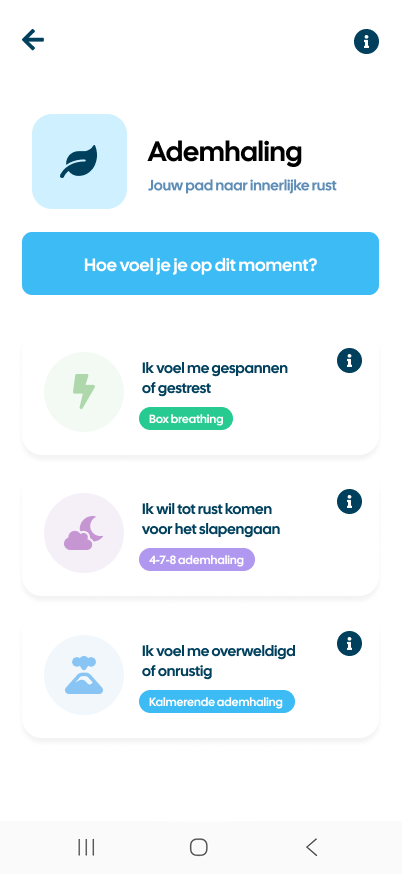
\includegraphics[width=\linewidth]{../graphics/Mockups/Oefeningen/ademhaling/Ademhaling1}
    \end{minipage}
    \hfill
    \begin{minipage}{0.3\textwidth}
        \centering
        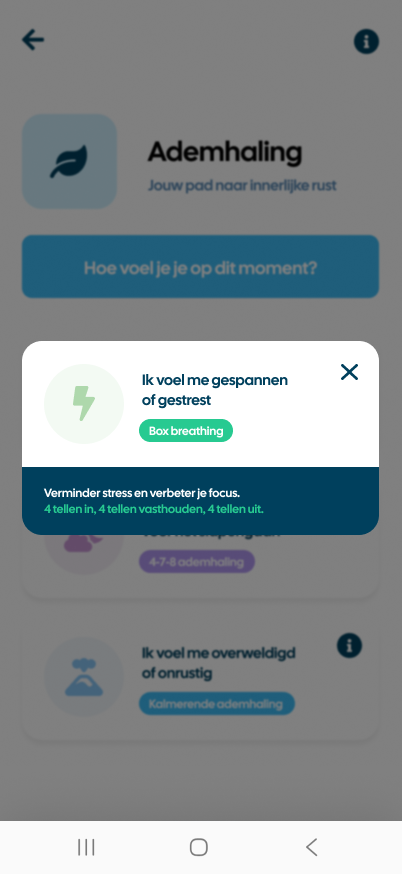
\includegraphics[width=\linewidth]{../graphics/Mockups/Oefeningen/ademhaling/Ademhaling2}
    \end{minipage}
    \hfill
    \begin{minipage}{0.3\textwidth}
        \centering
        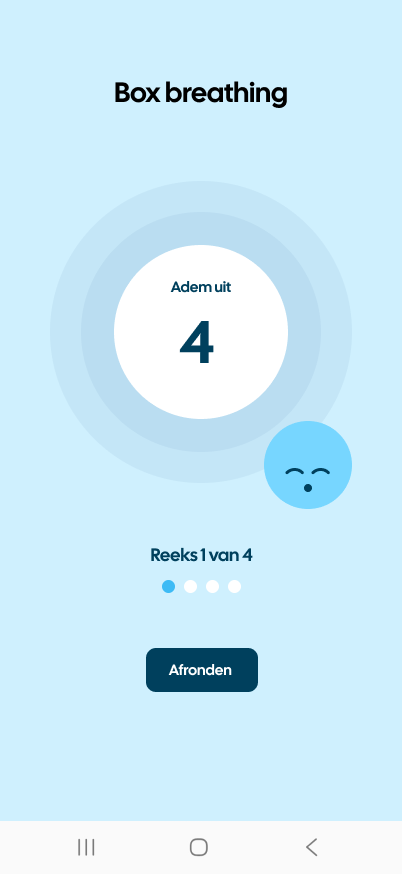
\includegraphics[width=\linewidth]{../graphics/Mockups/Oefeningen/ademhaling/Ademhaling3}
    \end{minipage}
    
    \caption{Mockups van ademhalingsoefeningen}
    \label{fig:mockups-5}
\end{figure}

{\small
    \begin{itemize}
        \item De oefeningen worden niet langer voornamelijk op basis van hun naam aangeboden, maar vanuit herkenbare behoeften, zoals spanning, onrust of de nood aan ontspanning voor het slapengaan. De naam van de gebruikte ademhalingstechniek wordt hierbij aanvullend weergegeven (\textbf{Ontwerpprincipe}: \textit{persoonlijke relevantie}).
        
        \item Via een informatieknop per oefening kan de gebruiker indien gewenst meer uitleg raadplegen over het doel en de opbouw van de ademhaling. Hierdoor blijft de basisweergave overzichtelijk zonder informatie weg te laten (\textbf{Ontwerpprincipe}: \textit{techno-simplicity}).
        
        \item Oefeningen die enkel beschikbaar waren binnen een betalend abonnement werden niet opgenomen. Hierdoor worden geen opties getoond die de gebruiker niet kan gebruiken, wat frustratie en onnodige informatie voorkomt (\textbf{Ontwerpprincipes}: \textit{minimaliseer cognitieve belasting}).
        
        \item Tijdens de oefening wordt enkel de functionele ademhalingsanimatie behouden. Overbodige bewegende elementen op de achtergrond werden verwijderd (\textbf{Ontwerpprincipe}: \textit{vermijd visuele overprikkeling}).
        
        \item Een digitale coach begeleidt de gebruiker tijdens de oefening en ademt mee. Dit biedt een vorm van begeleiding zonder prestatiedruk en ondersteunt de gebruiker tijdens het uitvoeren van de oefening (\textbf{Ontwerpprincipe}: \textit{betekenisvolle, prestatievrije motivatie}).
        
        \item Na afloop krijgt de gebruiker feedback over de voltooide oefening en wordt kort toegelicht wat werd bereikt. Een \textit{wist-je-datje} biedt hierbij aanvullende, relevante informatie (\textbf{Ontwerpprincipes}: \textit{ondersteun competentiegevoel, zichtbare meerwaarde}).
    \end{itemize}
}

\vspace{1em}

\subsubsection{Focus modus}
\label{subsubsec:focus-mockups}

\begin{figure}[H]
    \centering
    
    \begin{minipage}{0.3\textwidth}
        \centering
        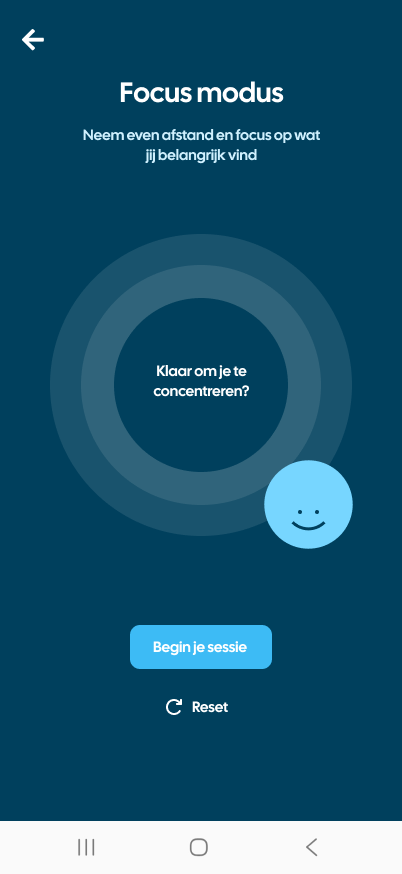
\includegraphics[width=\linewidth]{../graphics/Mockups/Oefeningen/focus/focus1}
    \end{minipage}
    \hfill
    \begin{minipage}{0.3\textwidth}
        \centering
        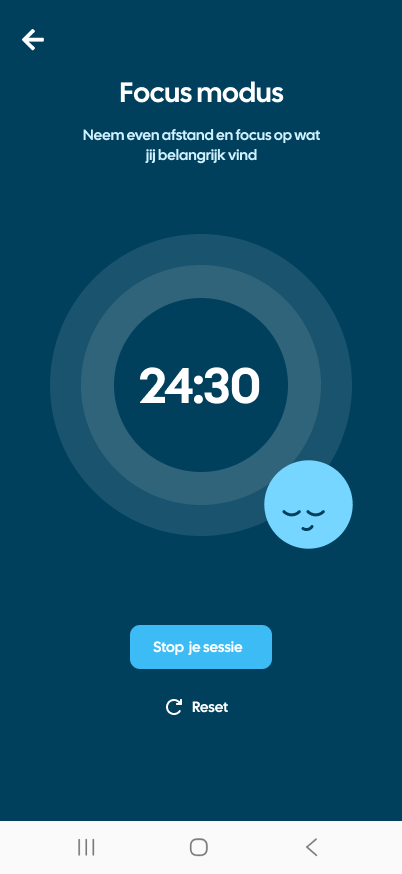
\includegraphics[width=\linewidth]{../graphics/Mockups/Oefeningen/focus/focus2}
    \end{minipage}
    \hfill
    \begin{minipage}{0.3\textwidth}
        \centering
        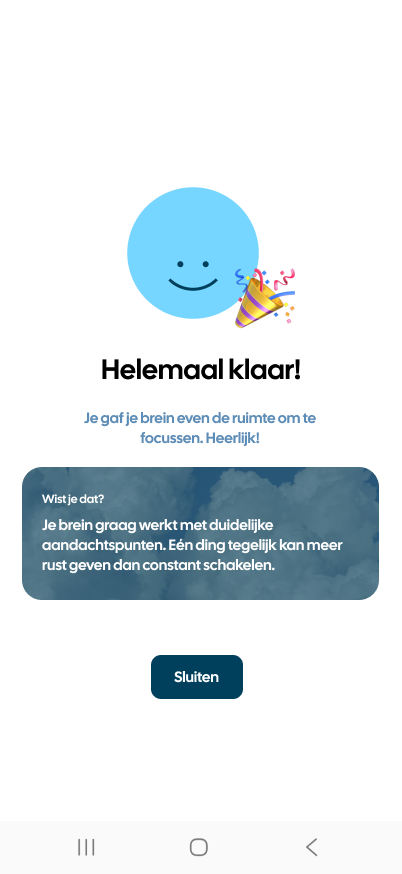
\includegraphics[width=\linewidth]{../graphics/Mockups/Oefeningen/focus/focus3}
    \end{minipage}
    
    \caption{Mockups van focus modus}
    \label{fig:mockups-6}
\end{figure}

In de vorige versie van de focusmodus (\ref{fig:burnout-free-5}) werd de gebruiker aangesproken met de boodschap \textit{“Stay productive, avoid burnout”}. Deze formulering legt sterk de nadruk op productiviteit en kan daardoor prestatiedruk oproepen. Daarnaast week de visuele vormgeving van de focustimer af van de andere oefeningen, waardoor de interface minder consistent aanvoelde. In de nieuwe versie werd daarom gekozen voor een meer ondersteunende en consistente aanpak.

\vspace{1em}

{\small
    \begin{itemize}
        \item De startpagina gebruikt ondersteunende communicatie die de gebruiker uitnodigt om bewust afstand te nemen en te focussen op wat voor hem of haar belangrijk is, zonder de nadruk te leggen op productiviteit (\textbf{Ontwerpprincipe}: \textit{ondersteunende communicatie}).
        
        \item Een digitale coach begeleidt de gebruiker tijdens de focussessie en biedt hierbij ondersteuning en gezelschap (\textbf{Ontwerpprincipe}: \textit{betekenisvolle, prestatievrije motivatie}).
        
        \item De timer volgt dezelfde visuele stijl als de andere oefeningen, waardoor een consistente ervaring over de verschillende functionaliteiten heen ontstaat (\textbf{Ontwerpprincipe}: \textit{behoud overzicht}).
        
        \item Na afloop krijgt de gebruiker feedback over de voltooide oefening en wordt kort toegelicht wat werd bereikt. Een \textit{wist-je-datje} biedt hierbij aanvullende, relevante informatie (\textbf{Ontwerpprincipes}: \textit{ondersteun competentiegevoel, zichtbare meerwaarde}).
    \end{itemize}
}

\vspace{1em}

\subsubsection{SOS modus}
\label{subsubsec:sos-mockups}

\begin{figure}[H]
    \centering
    
    \begin{minipage}{0.3\textwidth}
        \centering
        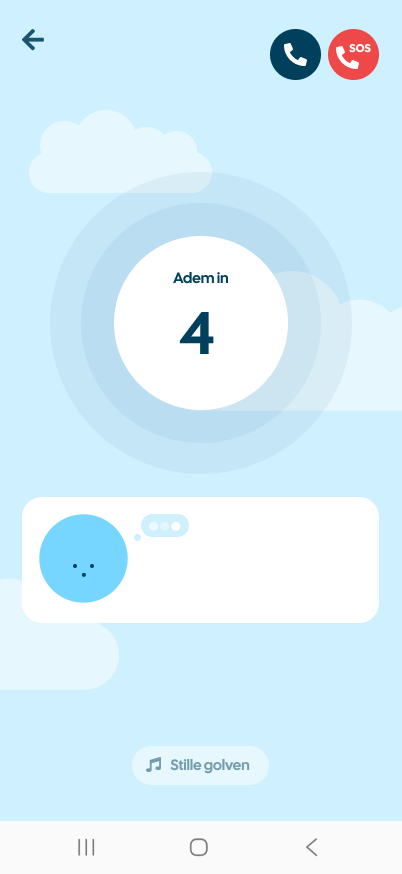
\includegraphics[width=\linewidth]{../graphics/Mockups/Oefeningen/sos/sos1}
    \end{minipage}
    \hfill
    \begin{minipage}{0.3\textwidth}
        \centering
        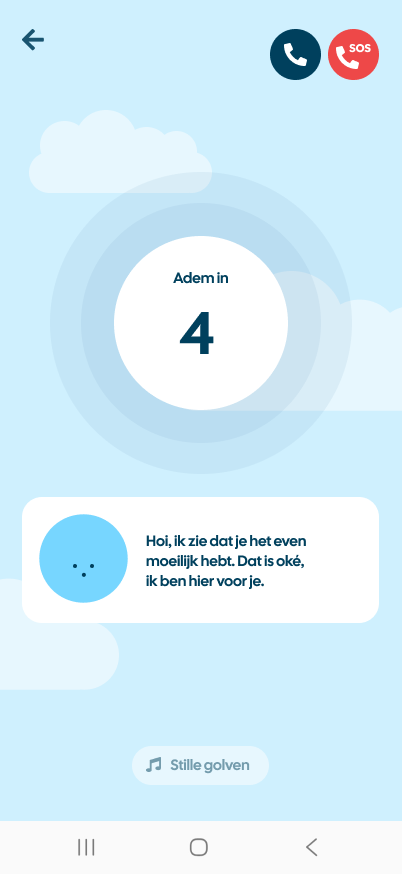
\includegraphics[width=\linewidth]{../graphics/Mockups/Oefeningen/sos/sos2}
    \end{minipage}
    \hfill
    \begin{minipage}{0.3\textwidth}
        \centering
        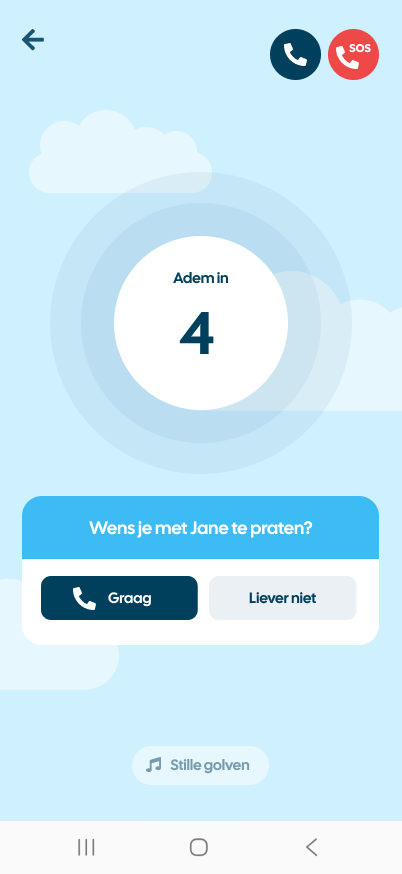
\includegraphics[width=\linewidth]{../graphics/Mockups/Oefeningen/sos/sos3}
    \end{minipage}
    
    \caption{Mockups van SOS modus}
    \label{fig:mockups-7}
\end{figure}

In de vorige versie van de SOS-modus werd voornamelijk een ademhalingsoefening aangeboden, aangevuld met korte geruststellende boodschappen. Daarnaast kon de gebruiker via een knop rechtsboven rechtstreeks contact opnemen met het ingestelde noodcontact. In de nieuwe versie werd de SOS-modus verder uitgebreid met meerdere vormen van ondersteuning en meer keuzevrijheid voor de gebruiker.

\vspace{1em}

{\small
    \begin{itemize}
        \item Het ingestelde noodcontact blijft rechtstreeks bereikbaar. Daarnaast werd een afzonderlijke optie voorzien om professionele hulp te contacteren wanneer het eigen netwerk onvoldoende ondersteuning kan bieden (\textbf{Ontwerpprincipe}: \textit{stimuleer authentieke verbondenheid}).
        
        \item De digitale coach biedt aanvullende ondersteuning en gezelschap, terwijl menselijk contact beschikbaar blijft. (\textbf{Ontwerpprincipe}: \textit{stimuleer authentieke verbondenheid}).
        
        \item Tijdens de begeleiding worden mogelijke acties voorgesteld, zoals contact opnemen met een vooraf ingesteld persoon. De gebruiker behoudt hierbij steeds de keuze om hier wel of niet op in te gaan (\textbf{Ontwerpprincipes}: \textit{ondersteun autonomie, zachte gedragssturing}).
    \end{itemize}
}

\vspace{1em}


\subsection{Dagboek}
\label{subsec:dagboek-mockups}

\begin{figure}[H]
    \centering
    
    \begin{minipage}{0.3\textwidth}
        \centering
        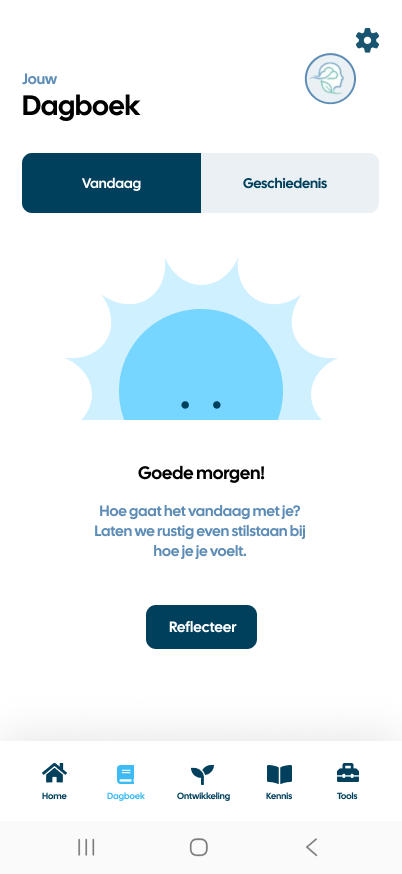
\includegraphics[width=\linewidth]{../graphics/Mockups/Journal/Dagboek_vandaag_nietIngevuld}
    \end{minipage}
    \hfill
    \begin{minipage}{0.3\textwidth}
        \centering
        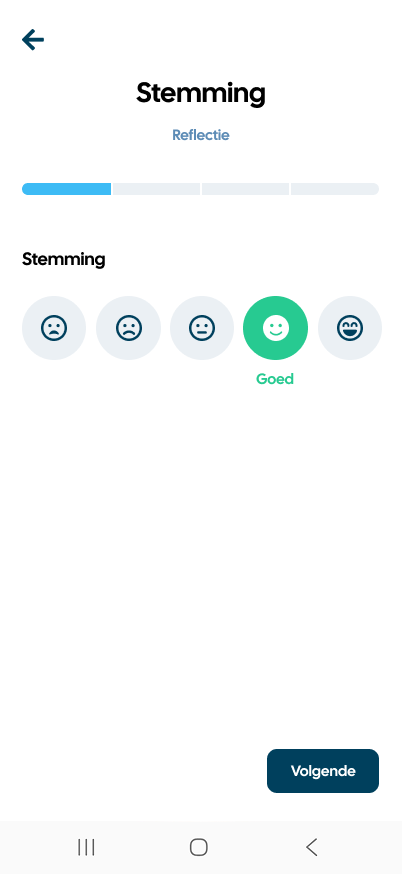
\includegraphics[width=\linewidth]{../graphics/Mockups/Journal/Dagboek_reflectie_slide1}
    \end{minipage}
    \hfill
    \begin{minipage}{0.3\textwidth}
        \centering
        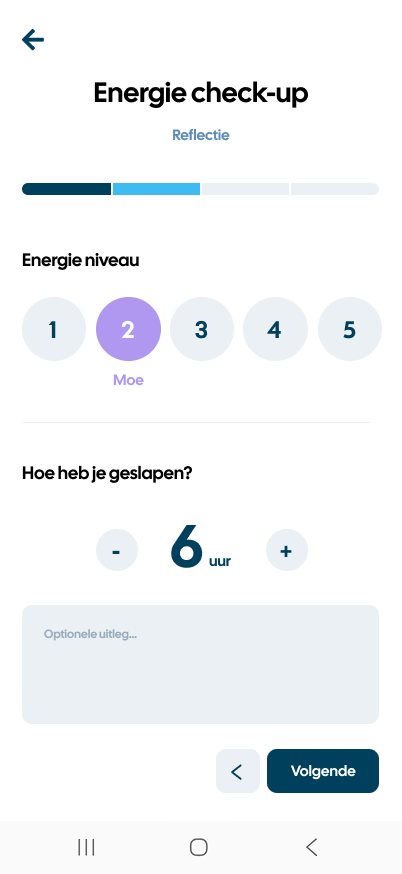
\includegraphics[width=\linewidth]{../graphics/Mockups/Journal/Dagboek_reflectie_slide2}
    \end{minipage}
    
    \vspace{1em}
    
    \begin{minipage}{0.3\textwidth}
        \centering
        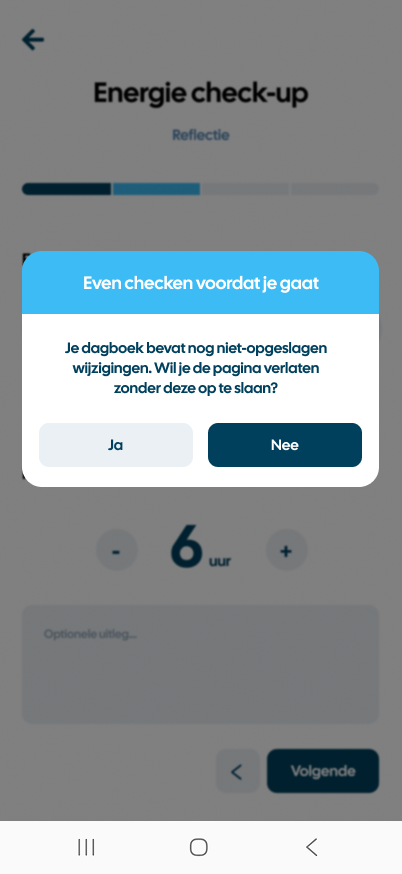
\includegraphics[width=\linewidth]{../graphics/Mockups/Journal/Dagboek_reflectie_slide3}
    \end{minipage}
    \hfill
    \begin{minipage}{0.3\textwidth}
        \centering
        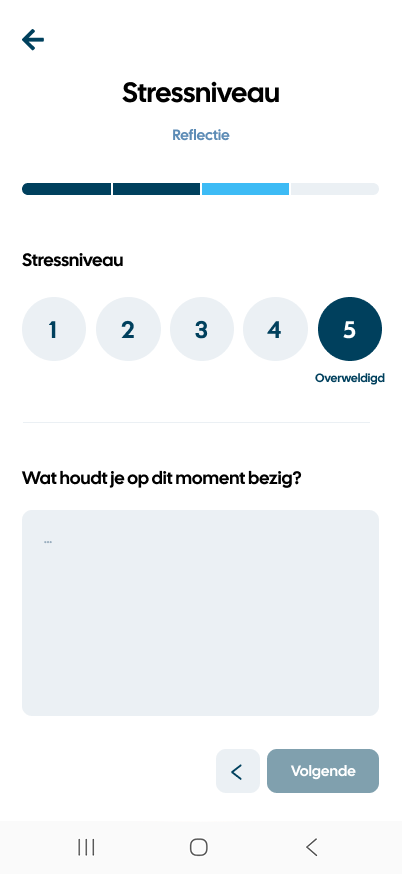
\includegraphics[width=\linewidth]{../graphics/Mockups/Journal/Dagboek_reflectie_slide4}
    \end{minipage}
    \hfill
    \begin{minipage}{0.3\textwidth}
        \centering
        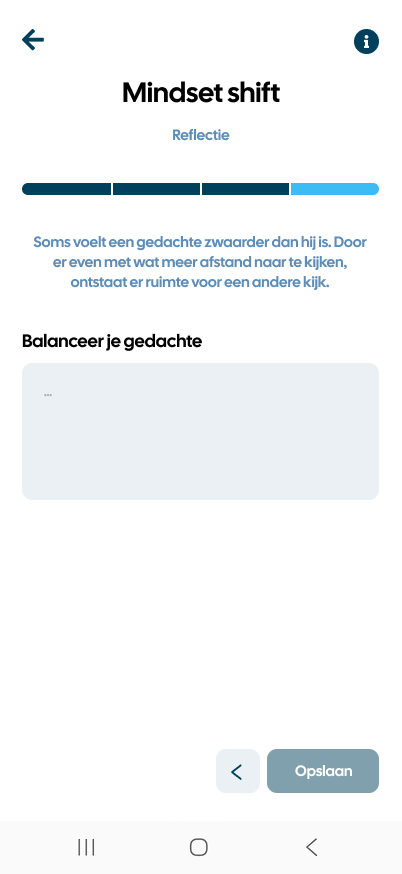
\includegraphics[width=\linewidth]{../graphics/Mockups/Journal/Dagboek_reflectie_slide5}
    \end{minipage}
    
    \caption{Mockups van het invullen van een dagboekreflectie}
    \label{fig:mockups-8}
\end{figure}

\begin{figure}[H]
    \centering
    
    \begin{minipage}{0.3\textwidth}
        \centering
        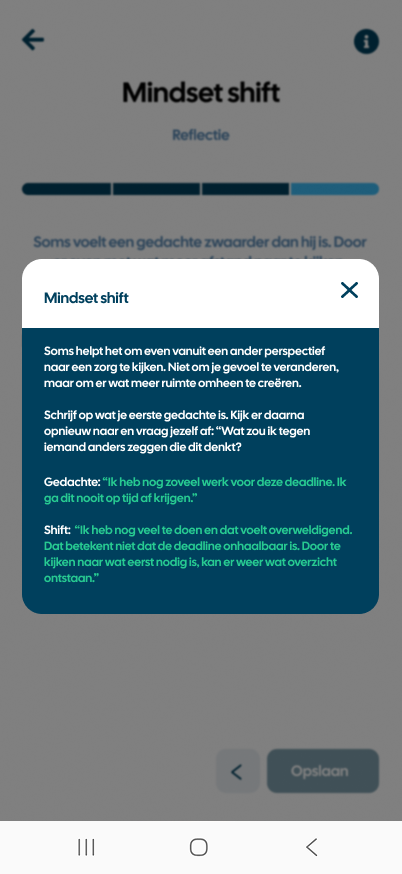
\includegraphics[width=\linewidth]{../graphics/Mockups/Journal/Dagboek_reflectie_slide6}
    \end{minipage}
    \hfill
    \begin{minipage}{0.3\textwidth}
        \centering
        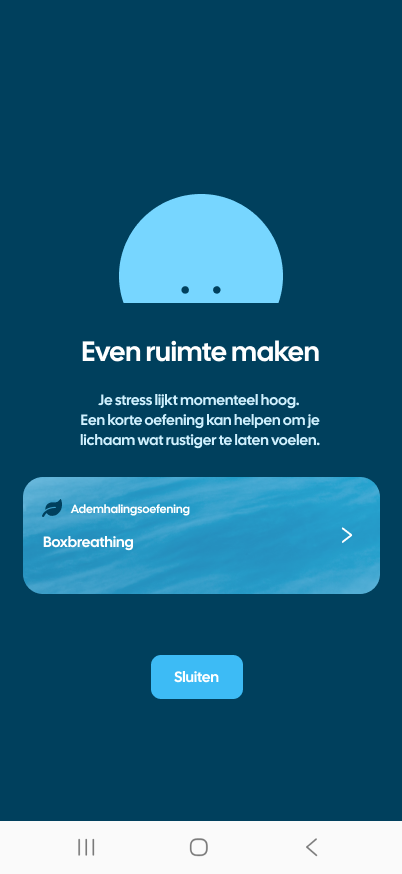
\includegraphics[width=\linewidth]{../graphics/Mockups/Journal/Dagboek_reflectie_slide7}
    \end{minipage}
    \hfill
    \begin{minipage}{0.3\textwidth}
        \centering
        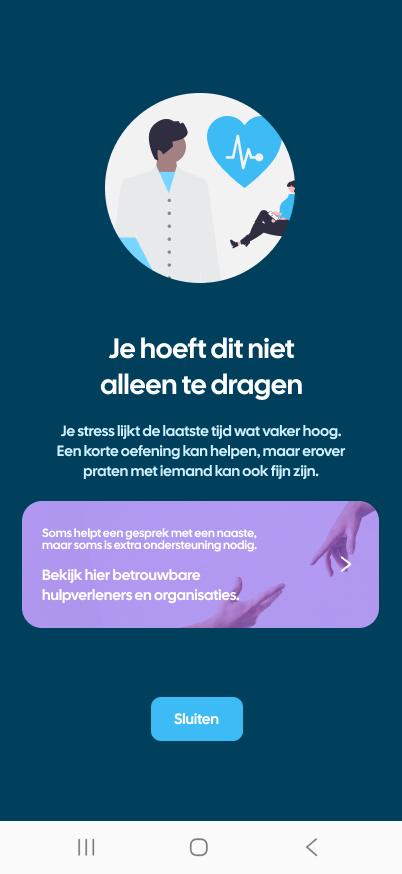
\includegraphics[width=\linewidth]{../graphics/Mockups/Journal/Dagboek_reflectie_slide8}
    \end{minipage}
    
    \vspace{1em}
    
    \begin{minipage}{0.3\textwidth}
        \centering
        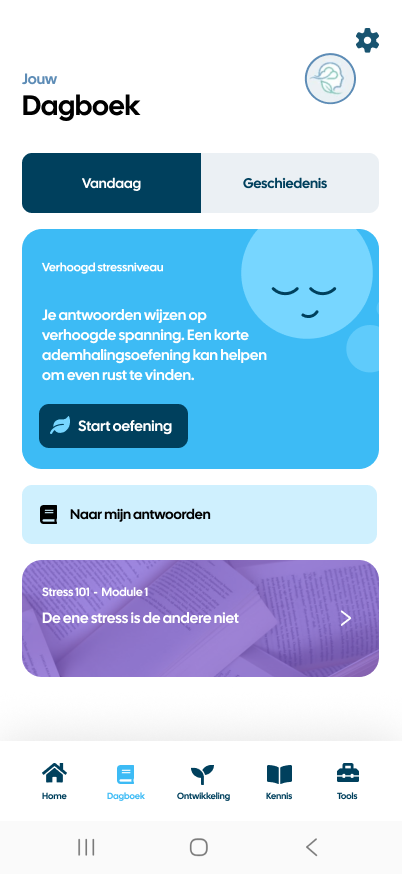
\includegraphics[width=\linewidth]{../graphics/Mockups/Journal/Dagboek_vandaag_ingevuld}
    \end{minipage}
    \hfill
    \begin{minipage}{0.3\textwidth}
        \centering
        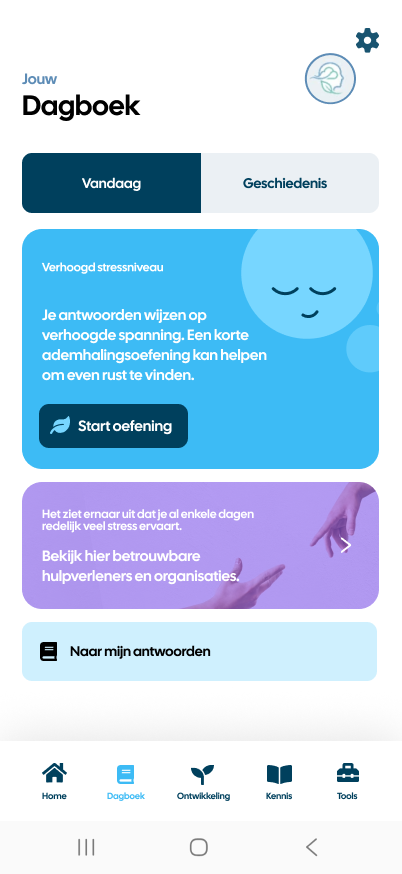
\includegraphics[width=\linewidth]{../graphics/Mockups/Journal/Dagboek_vandaag_ingevuld_langdurigeStress}
    \end{minipage}
    \hfill
    \begin{minipage}{0.3\textwidth}
        \centering
        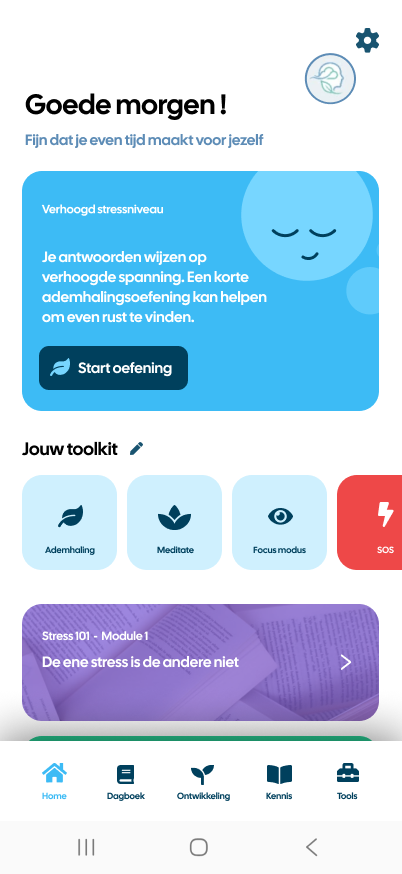
\includegraphics[width=\linewidth]{../graphics/Mockups/Journal/Dagboek_vandaag_ingevuld_home_oefening}
    \end{minipage}
    
    \caption{Mockups van het afronden van een dagboekreflectie en gepersonaliseerde opvolging}
    \label{fig:mockups-9}
\end{figure}

\begin{figure}[H]
    \centering
    
    % Linker afbeelding: neemt twee rijen in
    \begin{minipage}{0.3\textwidth}
        \centering
        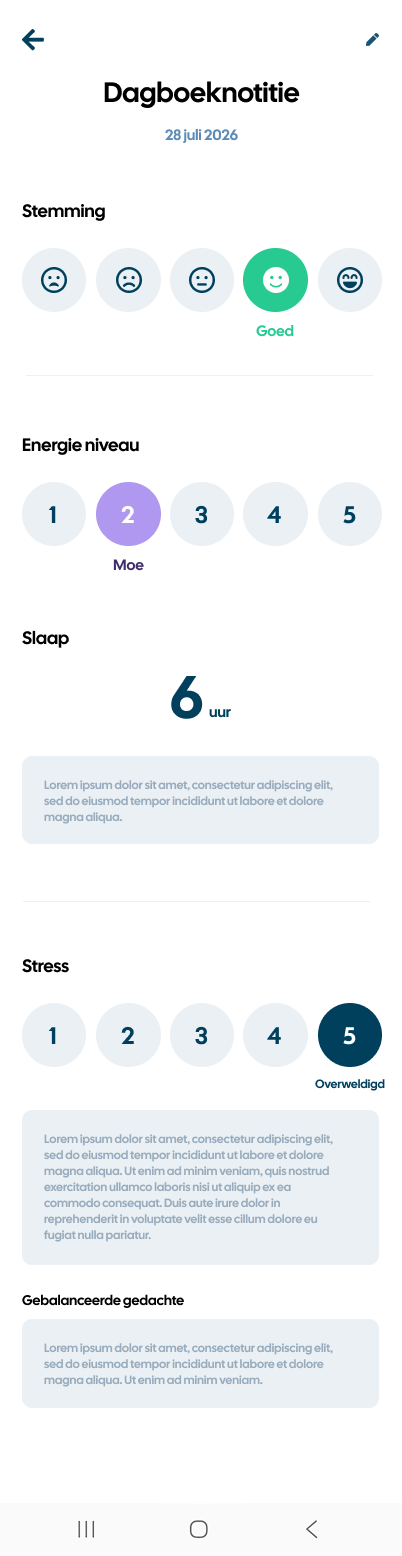
\includegraphics[width=\linewidth]{../graphics/Mockups/Journal/Dagboek_dagboeknotitie}
    \end{minipage}
    \hfill
    % Rechterkant: 2x2
    \begin{minipage}{0.63\textwidth}
        \centering
        
        % Bovenste rij
        \begin{minipage}{0.47\textwidth}
            \centering
            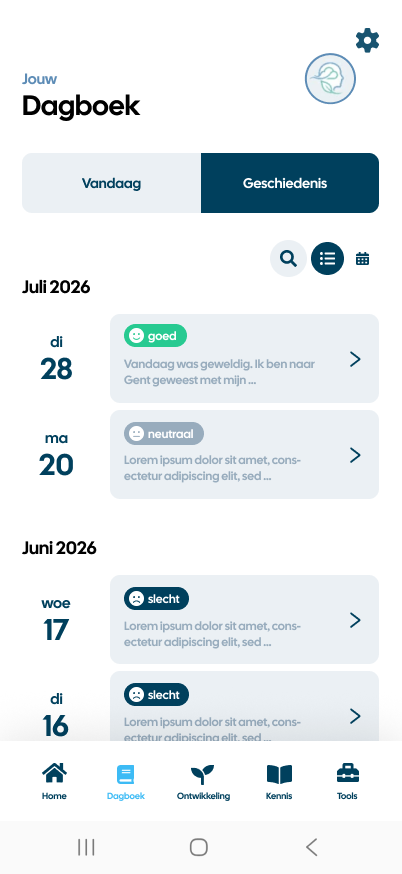
\includegraphics[width=\linewidth]{../graphics/Mockups/Journal/Dagboek_geschiedenis_lijst}
        \end{minipage}
        \hfill
        \begin{minipage}{0.47\textwidth}
            \centering
            \phantom{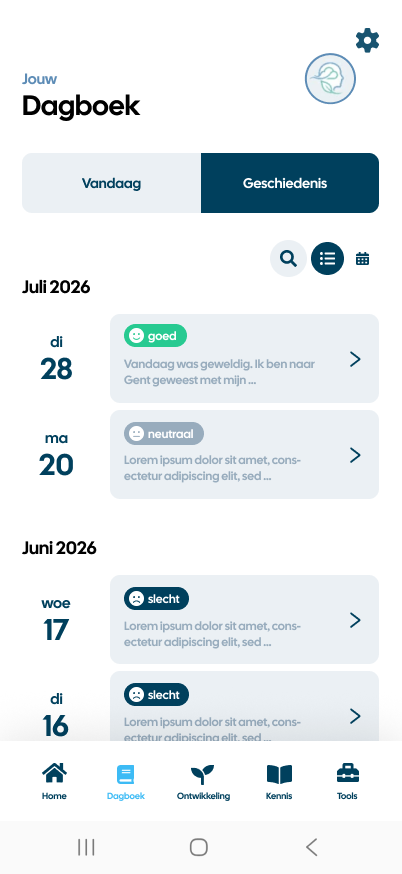
\includegraphics[width=\linewidth]{../graphics/Mockups/Journal/Dagboek_geschiedenis_lijst}}
        \end{minipage}
        
        \vspace{1em}
        
        % Onderste rij
        \begin{minipage}{0.47\textwidth}
            \centering
            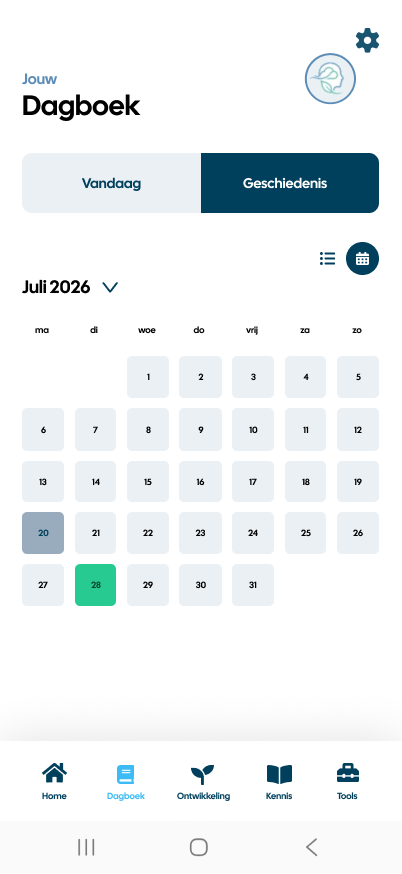
\includegraphics[width=\linewidth]{../graphics/Mockups/Journal/Dagboek_geschiedenis_kalender}
        \end{minipage}
        \hfill
        \begin{minipage}{0.47\textwidth}
            \centering
            \phantom{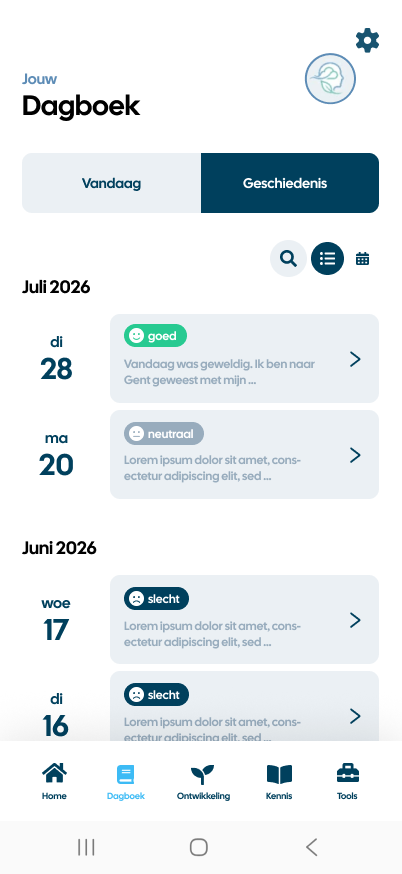
\includegraphics[width=\linewidth]{../graphics/Mockups/Journal/Dagboek_geschiedenis_lijst}}
        \end{minipage}
    \end{minipage}
    
    \caption{Mockups van de dagboeknotitie detailpagina en de historiek}
    \label{fig:mockups-10}
\end{figure}

\newpage

In de vorige versie (\ref{fig:burnout-free-1}) van de applicatie bestond het dagboek uit één scherm waarop de gebruiker verschillende gegevens kon invullen: stemming, energieniveau, aantal uren slaap en optioneel een notitie. Deze informatie werd op één pagina aangeboden, waarna de gebruiker de ingevulde gegevens kon opslaan. Er was echter geen mogelijkheid om eerdere dagboekentries terug te bekijken of om de evolutie ervan te raadplegen. Na het opslaan kreeg de gebruiker bovendien enkel een bevestiging dat de gegevens waren opgeslagen. Hierdoor bleef de meerwaarde van het bijhouden van deze informatie beperkt.

\vspace{1em}

{\small
    \begin{itemize}
        \item Het invullen van het dagboek werd opgesplitst in verschillende stappen en inhoudelijke categorieën, namelijk stemming, energie, stressniveau en mindset shift. Hierdoor wordt de hoeveelheid informatie per scherm beperkt en kan de gebruiker zich telkens op één aspect concentreren (\textbf{Ontwerpprincipe}: \textit{minimaliseer cognitieve belasting}).
        
        \item De oorspronkelijke slaapmeting bevatte naast het aantal uren slaap ook een extra visuele indicatie die aangaf of dit aantal uren "laag" of "hoog" was. Deze informatie voegde weinig toe, aangezien de gebruiker de slaapduur zelf al kon aflezen en de beoordeling bovendien weinig context bood. In de nieuwe versie werd dit vervangen door de bredere vraag \textit{"Hoe heb je geslapen?"}, waarbij de gebruiker het aantal uren kan opgeven en optioneel extra context over de slaap kan toevoegen. Hierdoor wordt overbodige informatie verwijderd en krijgt de gebruiker meer ruimte om de eigen situatie te beschrijven (\textbf{Ontwerpprincipes}: \textit{minimaliseer cognitieve belasting, persoonlijke relevantie}).
        
        \item Wanneer de gebruiker tijdens het invullen per ongeluk terug navigeert, wordt gevraagd of de reflectie moet worden verlaten zonder deze op te slaan. Hierdoor wordt onbedoeld gegevensverlies voorkomen en krijgt de gebruiker controle over deze actie (\textbf{Ontwerpprincipes}: \textit{ondersteunende foutafhandeling, ondersteun autonomie}).
        
        \item De gebruiker kan aangeven waarover hij of zij stress ervaart. Hierdoor wordt meer context verzameld over de persoonlijke situatie, waardoor de verdere begeleiding beter op de gebruiker kan worden afgestemd (\textbf{Ontwerpprincipe}: \textit{persoonlijke relevantie}).
        
        \item Op basis van de literatuurstudie werd een mindset shift toegevoegd, geïnspireerd door de toepassing van \acrshort{rebt}. De gebruiker wordt hierbij uitgenodigd om een stressvolle gedachte kritisch te bekijken en te herformuleren. Via een informatieknop kan bijkomende uitleg worden geraadpleegd over hoe deze oefening kan worden uitgevoerd, zodat de gebruiker niet zonder context met deze techniek wordt geconfronteerd (\textbf{Ontwerpprincipes}: \textit{ondersteun competentiegevoel, techno-simplicity}).
        
        \item Na het invullen van de reflectie ontvangt de gebruiker, indien relevant, een persoonlijke aanbeveling voor een passende oefening. Hierdoor wordt de geregistreerde informatie niet enkel opgeslagen, maar rechtstreeks vertaald naar mogelijke ondersteuning (\textbf{Ontwerpprincipes}: \textit{persoonlijke relevantie, zichtbare meerwaarde, zachte gedragssturing}).
        
        \item Wanneer uit meerdere dagboekentries een aanhoudende negatieve trend blijkt, bijvoorbeeld een langere periode met verhoogde stress, kan de applicatie de gebruiker aanraden om professionele hulp te zoeken. Hierdoor wordt niet enkel op een individueel moment gereageerd, maar kan ook rekening worden gehouden met patronen over tijd (\textbf{Ontwerpprincipes}: \textit{persoonlijke relevantie, ondersteunende communicatie}).
        
        \item De persoonlijke aanbevelingen worden ook zichtbaar gemaakt op het tabblad \textit{Vandaag} en op de homepagina. Hierdoor blijft de meerwaarde van het invullen van het dagboek zichtbaar en wordt de gebruiker op een laagdrempelige manier naar relevante ondersteuning geleid (\textbf{Ontwerpprincipes}: \textit{zichtbare meerwaarde, zachte gedragssturing}).
        
        \item Tot slot werd een \textit{Geschiedenis}-tabblad toegevoegd waarin eerdere dagboekentries zowel in een lijst- als kalenderweergave kunnen worden geraadpleegd. Door een eerdere entry te openen, kan de gebruiker zijn of haar antwoorden opnieuw bekijken en zo persoonlijke patronen of veranderingen herkennen (\textbf{Ontwerpprincipes}: \textit{ondersteun competentiegevoel, persoonlijke relevantie, zichtbare meerwaarde, behoud overzicht}).
    \end{itemize}
}

\newpage


\subsection{Ontwikkeling}
\label{subsec:ontwikkeling-mockups}

\begin{figure}[H]
    \centering
    
    \begin{minipage}{0.3\textwidth}
        \centering
        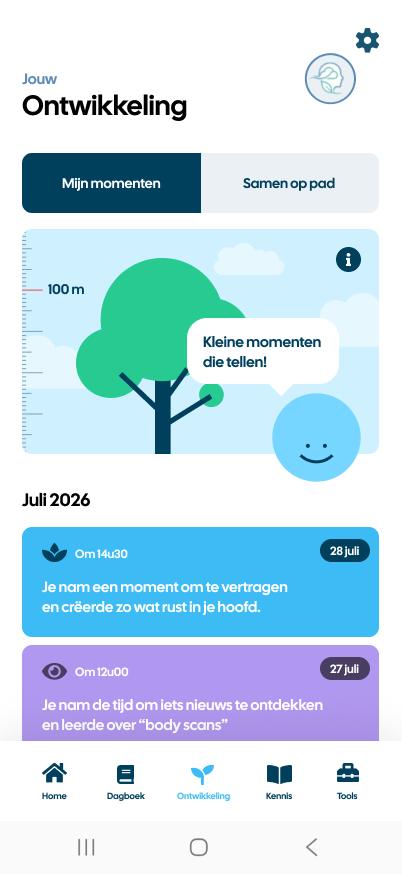
\includegraphics[width=\linewidth]{../graphics/Mockups/Ontwikkeling/Ontwikkeling_mijnMomenten}
    \end{minipage}
    \hfill
    \begin{minipage}{0.3\textwidth}
        \centering
        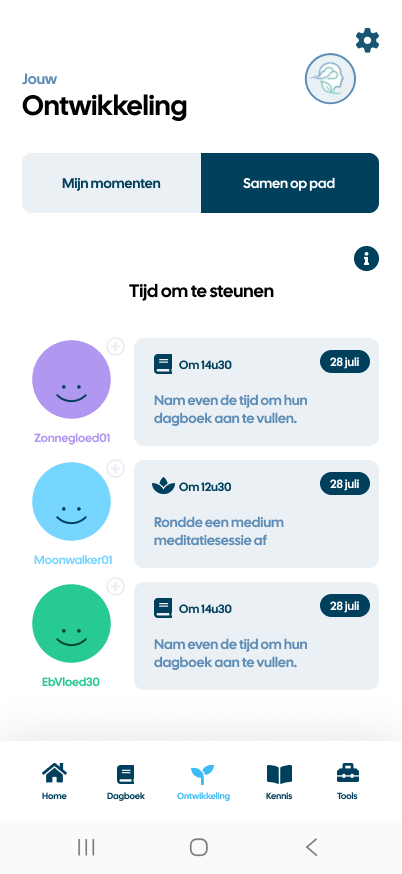
\includegraphics[width=\linewidth]{../graphics/Mockups/Ontwikkeling/Ontwikkeling_samenOpPad}
    \end{minipage}
    \hfill
    \begin{minipage}{0.3\textwidth}
        \centering
        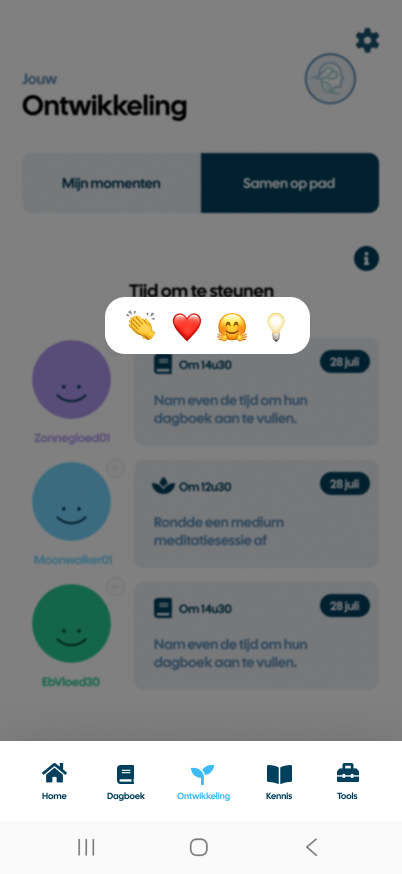
\includegraphics[width=\linewidth]{../graphics/Mockups/Ontwikkeling/Ontwikkeling_samenOpPad_2}
    \end{minipage}
    
    \vspace{1em}
    
    \begin{minipage}{0.3\textwidth}
        \centering
        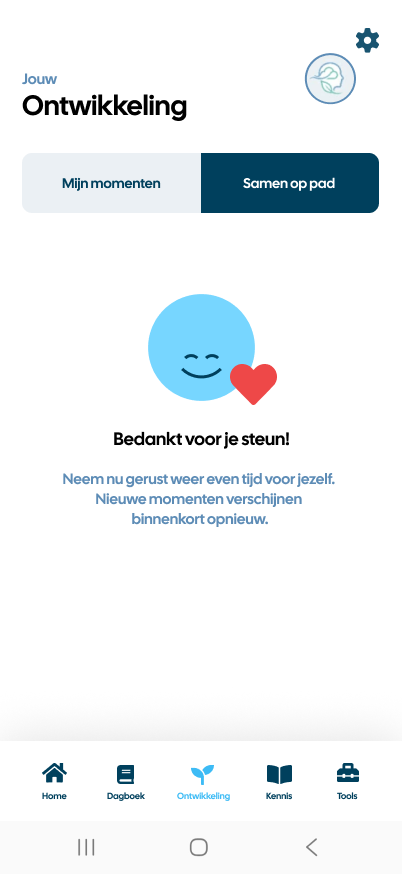
\includegraphics[width=\linewidth]{../graphics/Mockups/Ontwikkeling/Ontwikkeling_samenOpPad_3}
    \end{minipage}
    \hfill
    \begin{minipage}{0.3\textwidth}
        \centering
        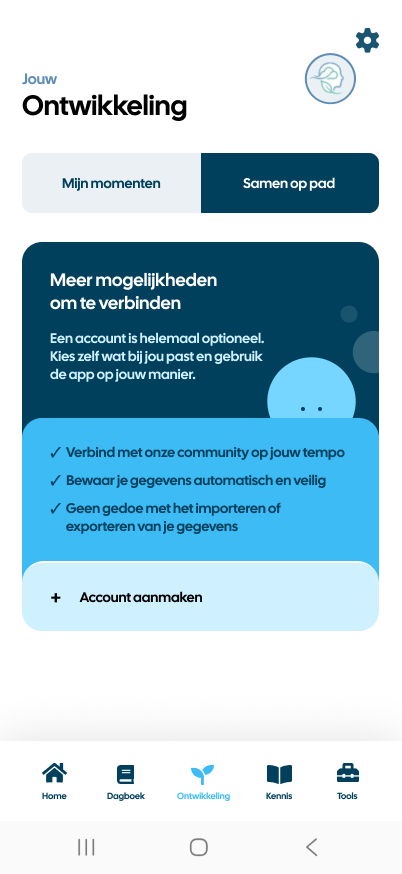
\includegraphics[width=\linewidth]{../graphics/Mockups/Ontwikkeling/Ontwikkeling_samenOpPad_4}
    \end{minipage}
    \hfill
    \begin{minipage}{0.3\textwidth}
        \centering
        \phantom{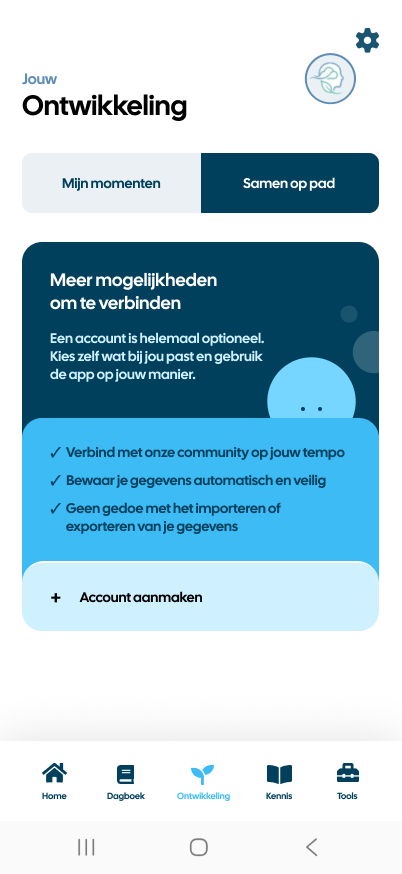
\includegraphics[width=\linewidth]{../graphics/Mockups/Ontwikkeling/Ontwikkeling_samenOpPad_4}}
    \end{minipage}
    
    \caption{Mockups van de ontwikkeling pagina}
    \label{fig:mockups-11}
\end{figure}

In de vorige versie van de applicatie was de voortgang voornamelijk zichtbaar via de statistiekenpagina. Hier werd de dagelijkse activiteit weergegeven aan de hand van een staafgrafiek, met een overzicht van respectievelijk zeven of dertig dagen. Deze weergave gaf weinig inzicht in wat de gebruiker concreet had bereikt en legde de nadruk voornamelijk op hoeveelheid en activiteit.

\vspace{1em}

{\small
    \begin{itemize}
        \item De statistiekenpagina werd vervangen door het tabblad \textit{Mijn momenten}, waarin activiteiten en kleine vooruitgangen van de gebruiker worden verzameld. Hierdoor wordt ook minimale vooruitgang zichtbaar (\textbf{Ontwerpprincipes}: \textit{betekenisvolle, prestatievrije motivatie, zichtbare meerwaarde}).
        
        \item De voortgang wordt visueel voorgesteld aan de hand van een groeiende boom. Naarmate de gebruiker meer activiteiten uitvoert, groeit de boom verder. Hierdoor wordt ontwikkeling zichtbaar zonder cijfers of prestatiedoelen. Een info-icoon geeft hierover bijkomende uitleg (\textbf{Ontwerpprincipes}: \textit{betekenisvolle, prestatievrije motivatie, ondersteun competentiegevoel}).
        
        \item De coach begeleidt de gebruiker binnen \textit{Mijn momenten} met korte boodschappen die de persoonlijke vooruitgang benadrukken (\textbf{Ontwerpprincipes}: \textit{betekenisvolle, prestatievrije motivatie, persoonlijke relevantie}).
        
        \item Daarnaast werd het tabblad \textit{Samen op pad} toegevoegd. Ingelogde gebruikers kunnen activiteiten van andere communityleden bekijken en hen aanmoedigen met vooraf bepaalde ondersteunende reacties. Dit stimuleert authentieke verbondenheid en beperkt ongewenste communicatie (\textbf{Ontwerpprincipes}: \textit{stimuleer authentieke verbondenheid, ondersteunende communicatie}).
        
        \item Bij het versturen van een aanmoediging wordt de gebruikersnaam van de ontvanger weergegeven. De ontvanger ziet daarentegen niet van welke gebruiker de aanmoediging afkomstig is, waardoor deze anoniem blijft (\textbf{Ontwerpprincipe}: \textit{Privacy by Design}).
        
        \item Om te vermijden dat een gebrek aan ontvangen aanmoedigingen als negatief wordt ervaren, voorziet de applicatie ook zelf in anonieme aanmoedigingen. Dit vormt een veiligheidsmechanisme wanneer de community nog weinig actief is (\textbf{Ontwerp- principes}: \textit{betekenisvolle, prestatievrije motivatie, stimuleer authentieke verbondenheid}).
        
        \item Het aantal activiteiten waarop een gebruiker kan reageren wordt beperkt om een eindeloze contentfeed en overmatig scrollen te vermijden (\textbf{Ontwerpprincipe}: \textit{stimuleer gezond gebruik}).
        
        \item Een info-icoon binnen \textit{Samen op pad} geeft bijkomende uitleg over de werking van de community en de anonieme aanmoedigingen (\textbf{Ontwerpprincipes}: \textit{minimaliseer cognitieve belasting, ondersteun autonomie}).
    \end{itemize}
}

\vspace{1em}


\subsection{Kennishoek}
\label{subsec:kennishoek-mockups}

\begin{figure}[H]
    \centering
    
    \begin{minipage}{0.3\textwidth}
        \centering
        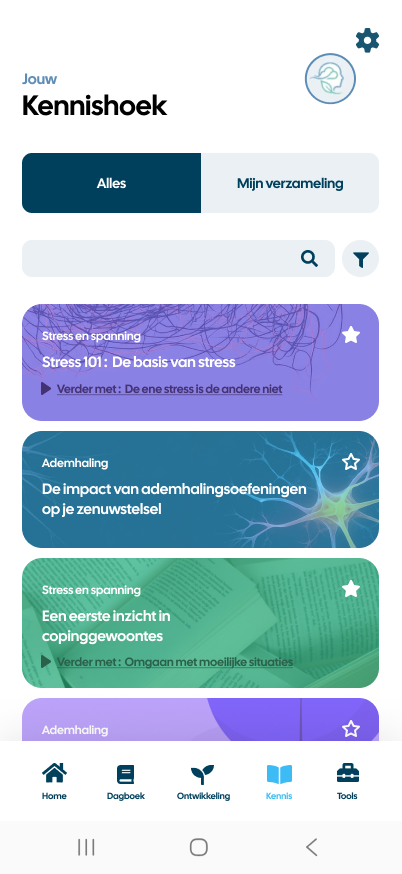
\includegraphics[width=\linewidth]{../graphics/Mockups/Kennis/Kennis_alles}
    \end{minipage}
    \hfill
    \begin{minipage}{0.3\textwidth}
        \centering
        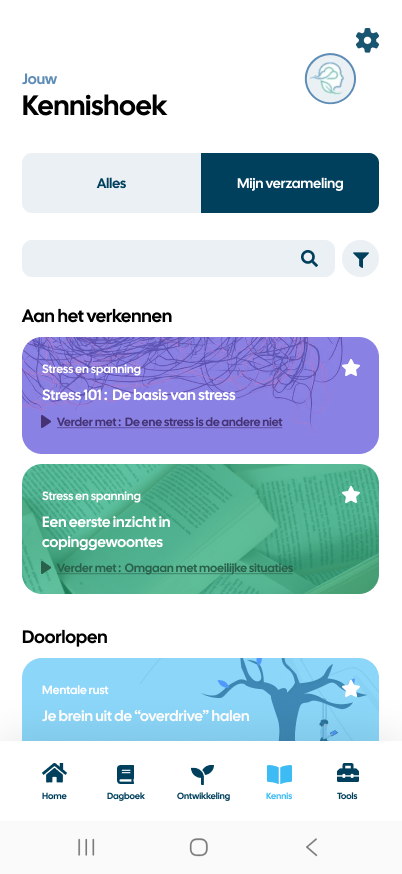
\includegraphics[width=\linewidth]{../graphics/Mockups/Kennis/Kennis_mijnVerzameling}
    \end{minipage}
    \hfill
    \begin{minipage}{0.3\textwidth}
        \centering
        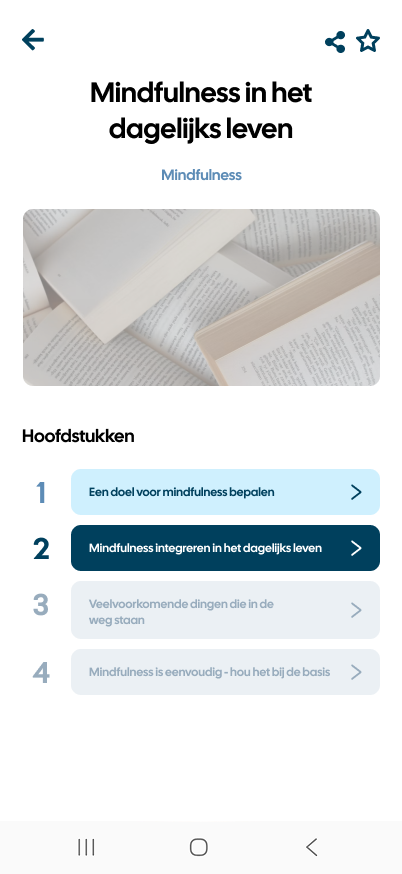
\includegraphics[width=\linewidth]{../graphics/Mockups/Kennis/Kennis_cursus}
    \end{minipage}
    
    \vspace{1em}
    
    \begin{minipage}{0.3\textwidth}
        \centering
        
\includegraphics[width=\linewidth]{../graphics/Mockups/Kennis/Kennis_cursus_inhoud1}
    \end{minipage}
    \hfill
    \begin{minipage}{0.3\textwidth}
        \centering
        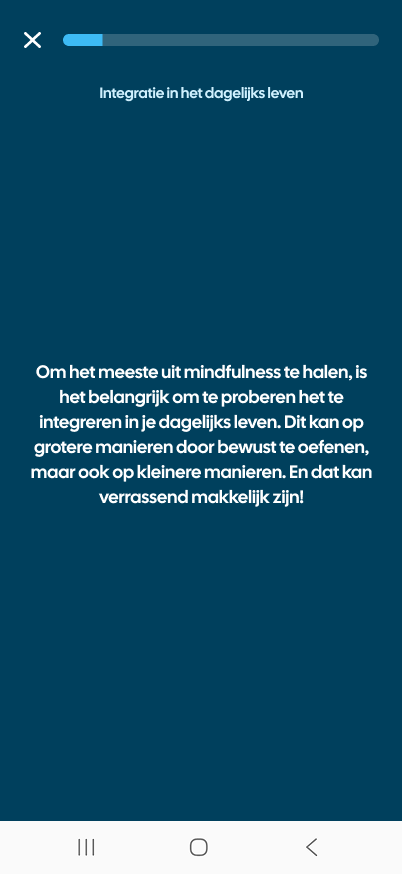
\includegraphics[width=\linewidth]{../graphics/Mockups/Kennis/Kennis_cursus_inhoud2}
    \end{minipage}
    \hfill
    \begin{minipage}{0.3\textwidth}
        \centering
        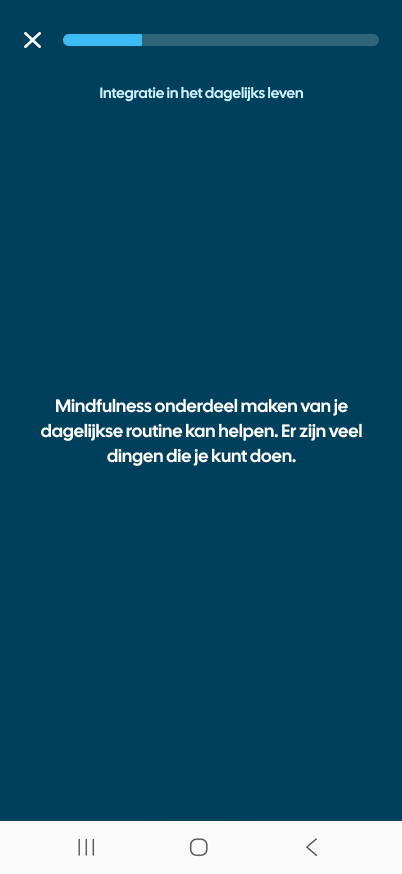
\includegraphics[width=\linewidth]{../graphics/Mockups/Kennis/Kennis_cursus_inhoud3}
    \end{minipage}
    
    \caption{Mockups van de kennishoek, een cursus en cursusinhoud}
    \label{fig:mockups-12}
\end{figure}

\begin{figure}[H]
    \centering
    
    \begin{minipage}{0.3\textwidth}
        \centering
        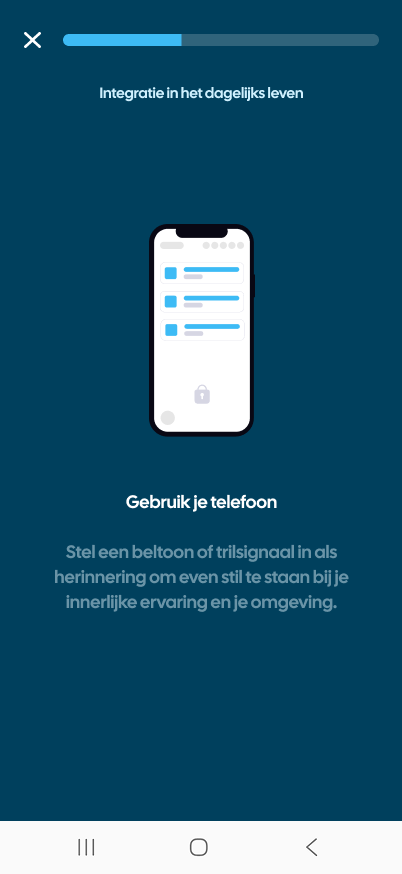
\includegraphics[width=\linewidth]{../graphics/Mockups/Kennis/Kennis_cursus_inhoud4}
    \end{minipage}
    \hfill
    \begin{minipage}{0.3\textwidth}
        \centering
        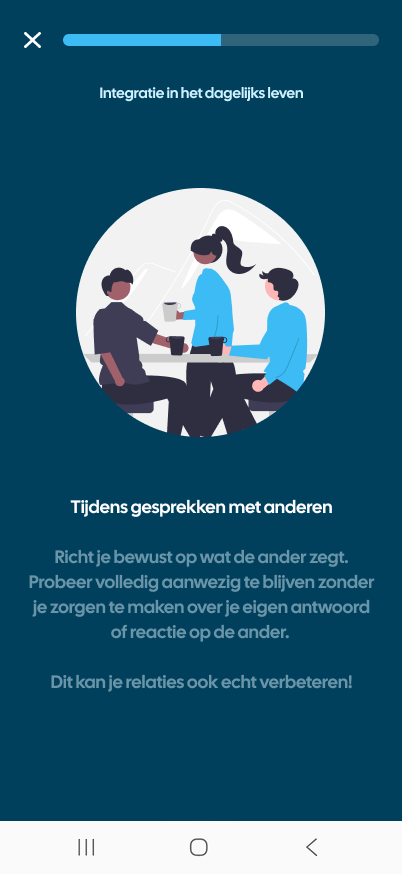
\includegraphics[width=\linewidth]{../graphics/Mockups/Kennis/Kennis_cursus_inhoud5}
    \end{minipage}
    \hfill
    \begin{minipage}{0.3\textwidth}
        \centering
        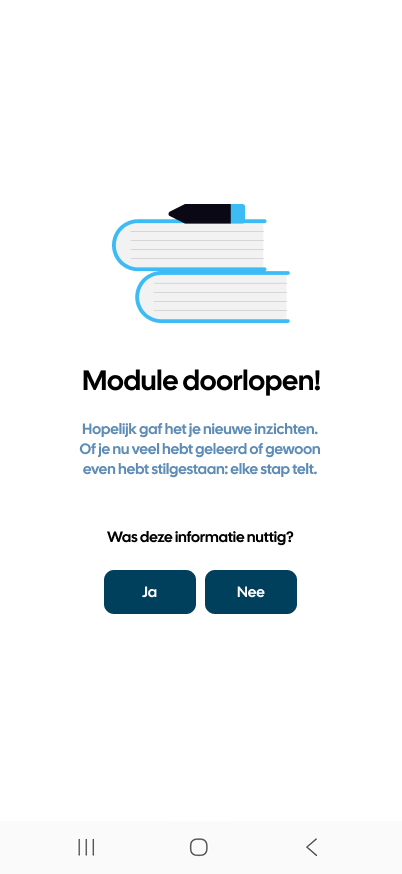
\includegraphics[width=\linewidth]{../graphics/Mockups/Kennis/Kennis_cursus_inhoud6}
    \end{minipage}
    
    \vspace{1em}
    
    \begin{minipage}{0.3\textwidth}
        \centering
        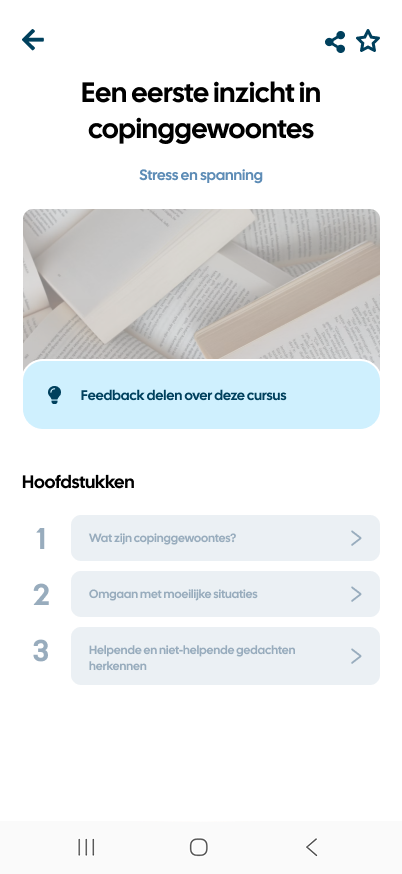
\includegraphics[width=\linewidth]{../graphics/Mockups/Kennis/Kennis_expert1}
    \end{minipage}
    \hfill
    \begin{minipage}{0.3\textwidth}
        \centering
        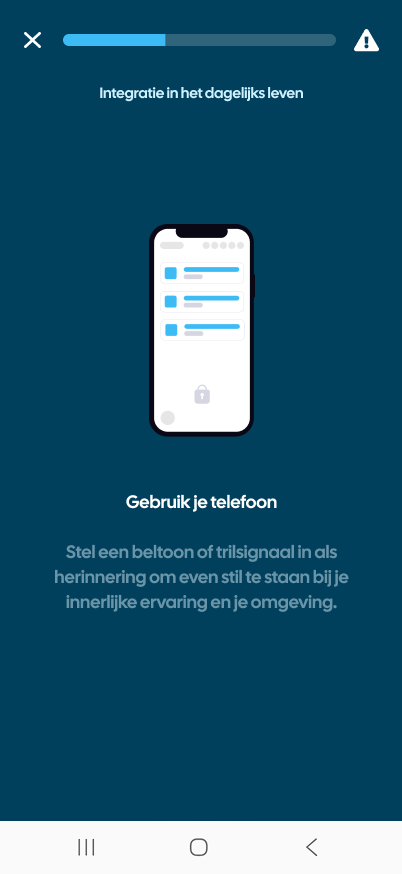
\includegraphics[width=\linewidth]{../graphics/Mockups/Kennis/Kennis_expert2}
    \end{minipage}
    \hfill
    \begin{minipage}{0.3\textwidth}
        \centering
        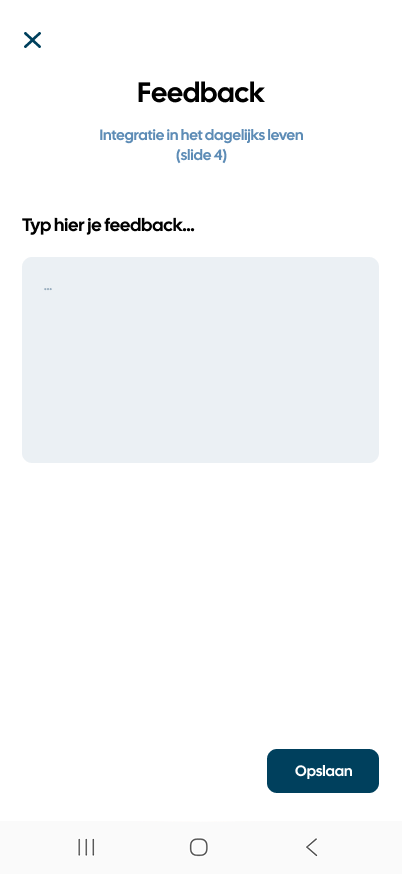
\includegraphics[width=\linewidth]{../graphics/Mockups/Kennis/Kennis_expert3}
    \end{minipage}
    
    \caption{Mockups van cursusinhoud (boven) en expertcontent binnen de kennishoek (onder)}
    \label{fig:mockups-13}
\end{figure}

\newpage

In de oorspronkelijke versie van de Burnout Free-app was geen kenniscontent of psycho-educatie aanwezig. Dit vormde een ontbrekende functionaliteit ten opzichte van de functionele requirements. Om te onderzoeken hoe dergelijke content op een toegankelijke manier kan worden aangeboden, werd gekeken naar de app Mindfulness Coach als vergelijkingspunt (\ref{fig:burnout-free-5}). De kenniscontent hiervan bestaat voornamelijk uit langere tekstuele pagina's, met weinig visuele ondersteuning, waardoor de informatie relatief zwaar en moeilijker te verwerken is.

\vspace{1em}

{\small
    \begin{itemize}
        \item De kennishoek werd opgebouwd rond cursussen die zijn opgesplitst in verschillende hoofdstukken. Hierdoor wordt de hoeveelheid informatie per onderdeel beperkt en kan de gebruiker de leerstof stapsgewijs doorlopen (\textbf{Ontwerpprincipes}: \textit{minimaliseer cognitieve belasting, ondersteun autonomie}).
        
        \item De hoofdstukken zijn vormgegeven als een visuele \textit{story}, waarbij korte stukken informatie stap voor stap worden aangeboden. Illustraties ondersteunen de tekst en zorgen voor meer afwisseling, waardoor de inhoud toegankelijker en beter behapbaar wordt (\textbf{Ontwerpprincipes}: \textit{minimaliseer cognitieve belasting, vermijd visuele overprikkeling}).
        
        \item Na het doorlopen van een hoofdstuk krijgt de gebruiker een korte terugkoppeling over wat werd bereikt en geleerd. Hierdoor wordt de meerwaarde van het doorlopen van de content expliciet gemaakt (\textbf{Ontwerpprincipe}: \textit{zichtbare meerwaarde}).
        
        \item Vervolgens kan de gebruiker aangeven of de informatie nuttig was. Deze feedback kan worden gebruikt om toekomstige aanbevelingen op de homepagina beter af te stemmen op de gebruiker (\textbf{Ontwerpprincipes}: \textit{persoonlijke relevantie, ondersteun autonomie}).
        
        \item Voor expertgebruikers werd de mogelijkheid voorzien om feedback te geven op de kenniscontent. Dit kan zowel op cursusniveau als specifiek op een afzonderlijke slide binnen een hoofdstuk, zodat feedback gericht kan worden gegeven op de volledige cursus of op een specifiek inhoudelijk onderdeel (\textbf{Ontwerpprincipes}: \textit{zichtbare meerwaarde, ondersteun autonomie}).
    \end{itemize}
}

\vspace{1em}


\subsection{Onboarding}
\label{subsec:onboarding-mockups}

\begin{figure}[H]
    \centering
    
    \begin{minipage}{0.3\textwidth}
        \centering
        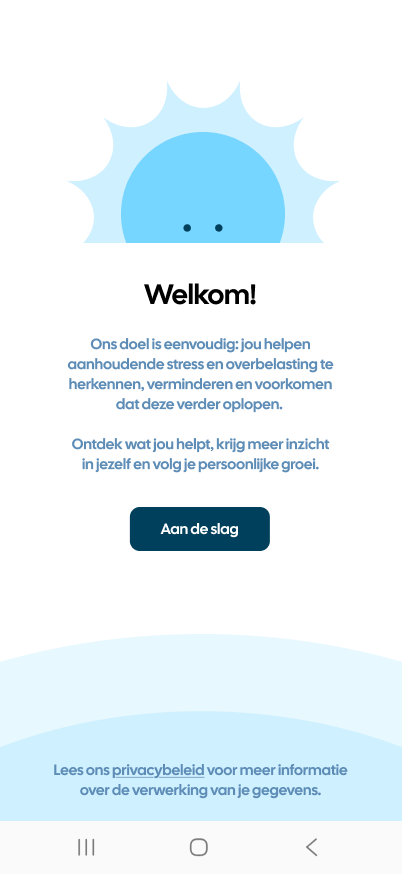
\includegraphics[width=\linewidth]{../graphics/Mockups/Onboarding/onboarding2}
    \end{minipage}
    \hfill
    \begin{minipage}{0.3\textwidth}
        \centering
        
\includegraphics[width=\linewidth]{../graphics/Mockups/Onboarding/onboarding3}
    \end{minipage}
    \hfill
    \begin{minipage}{0.3\textwidth}
        \centering
        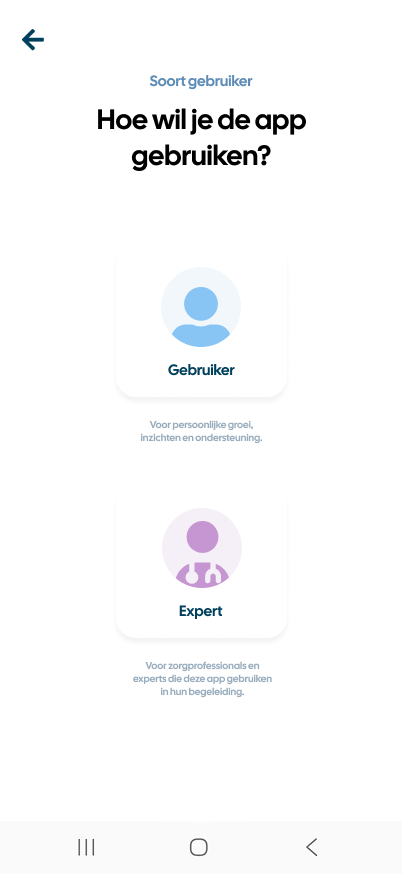
\includegraphics[width=\linewidth]{../graphics/Mockups/Onboarding/onboarding4}
    \end{minipage}
    
    \vspace{1em}
    
    \begin{minipage}{0.3\textwidth}
        \centering
        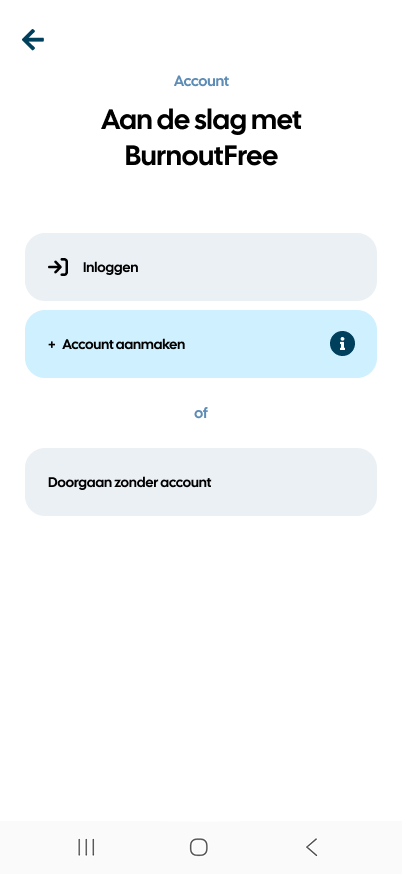
\includegraphics[width=\linewidth]{../graphics/Mockups/Onboarding/onboarding5}
    \end{minipage}
    \hfill
    \begin{minipage}{0.3\textwidth}
        \centering
        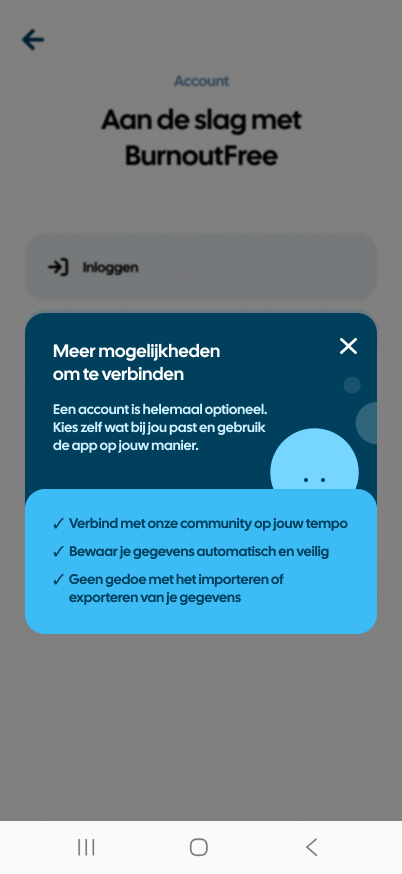
\includegraphics[width=\linewidth]{../graphics/Mockups/Onboarding/onboarding6}
    \end{minipage}
    \hfill
    \begin{minipage}{0.3\textwidth}
        \centering
        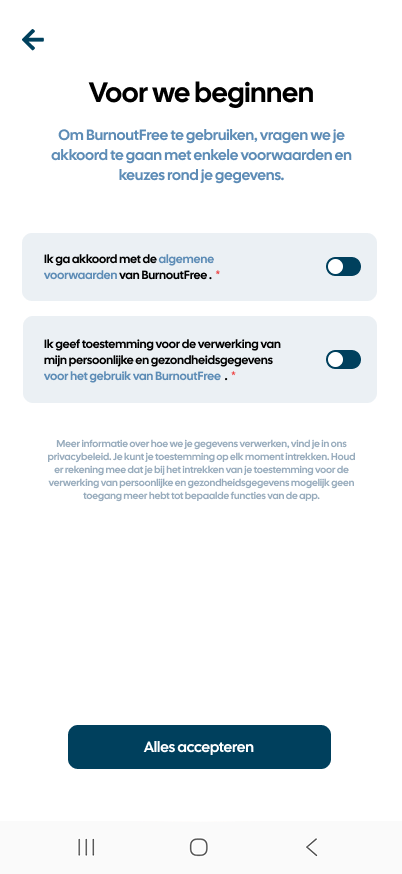
\includegraphics[width=\linewidth]{../graphics/Mockups/Onboarding/onboarding7}
    \end{minipage}
    
    \caption{Mockups van het begin van de onboarding: welkom, professionele hulp, gebruiksoptie, accountkeuze en toestemmingen}
    \label{fig:mockups-14}
\end{figure}

\begin{figure}[H]
    \centering
    
    \begin{minipage}{0.3\textwidth}
        \centering
        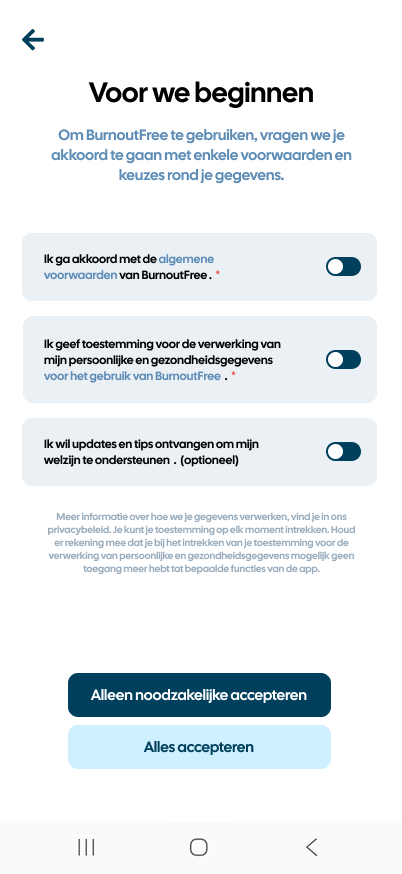
\includegraphics[width=\linewidth]{../graphics/Mockups/Onboarding/onboarding8}
    \end{minipage}
    \hfill
    \begin{minipage}{0.3\textwidth}
        \centering
        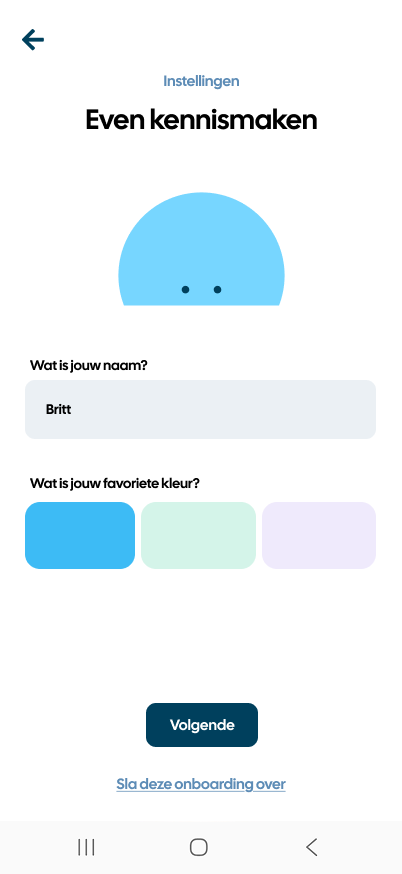
\includegraphics[width=\linewidth]{../graphics/Mockups/Onboarding/onboarding9}
    \end{minipage}
    \hfill
    \begin{minipage}{0.3\textwidth}
        \centering
        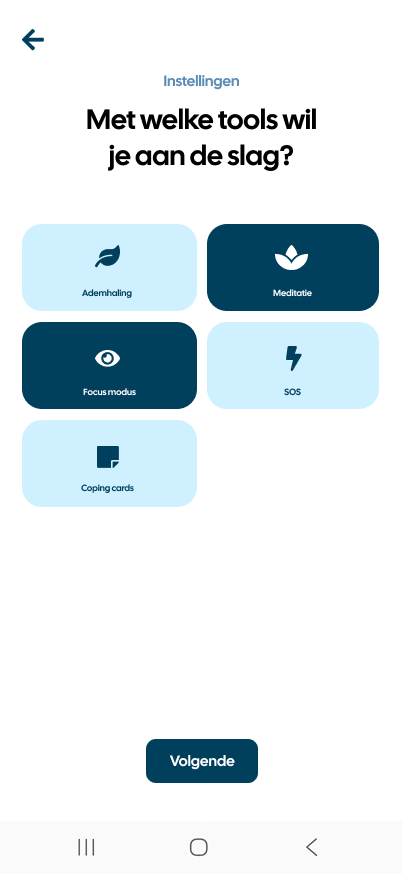
\includegraphics[width=\linewidth]{../graphics/Mockups/Onboarding/onboarding10}
    \end{minipage}
    
    \vspace{1em}
    
    \begin{minipage}{0.3\textwidth}
        \centering
        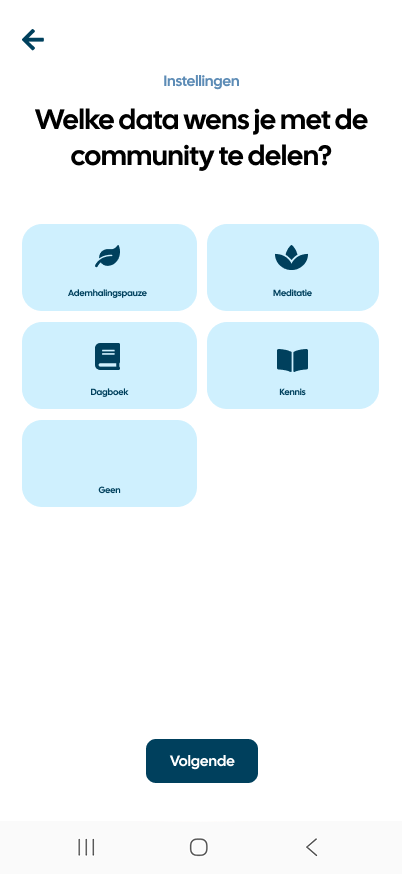
\includegraphics[width=\linewidth]{../graphics/Mockups/Onboarding/onboarding11}
    \end{minipage}
    \hfill
    \begin{minipage}{0.3\textwidth}
        \centering
        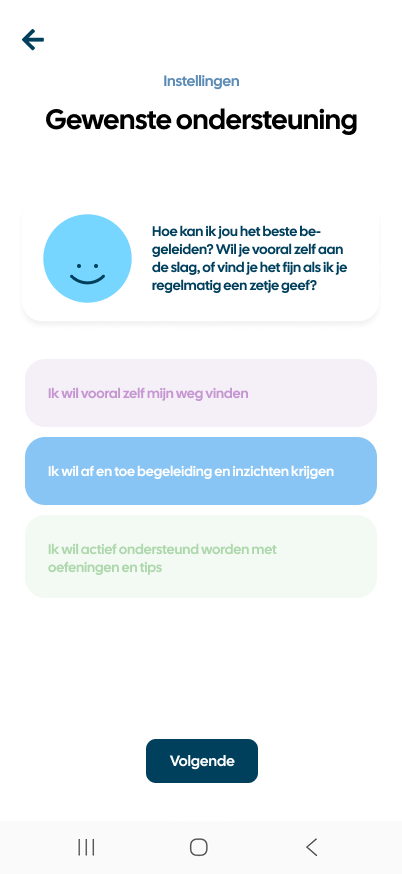
\includegraphics[width=\linewidth]{../graphics/Mockups/Onboarding/onboarding12}
    \end{minipage}
    \hfill
    \begin{minipage}{0.3\textwidth}
        \centering
        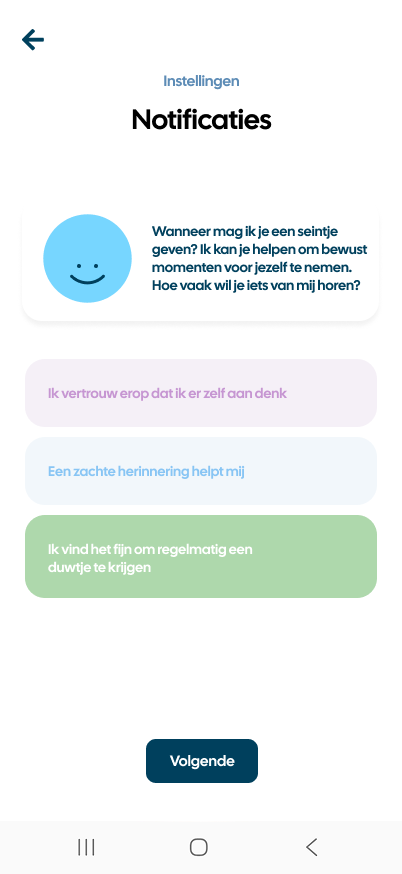
\includegraphics[width=\linewidth]{../graphics/Mockups/Onboarding/onboarding13}
    \end{minipage}
    
    \caption{Mockups van het personaliseren van de applicatie en het instellen van ondersteuning, communitygegevens en notificaties}
    \label{fig:mockups-15}
\end{figure}

\begin{figure}[H]
    \centering
    
    \begin{minipage}{0.3\textwidth}
        \centering
        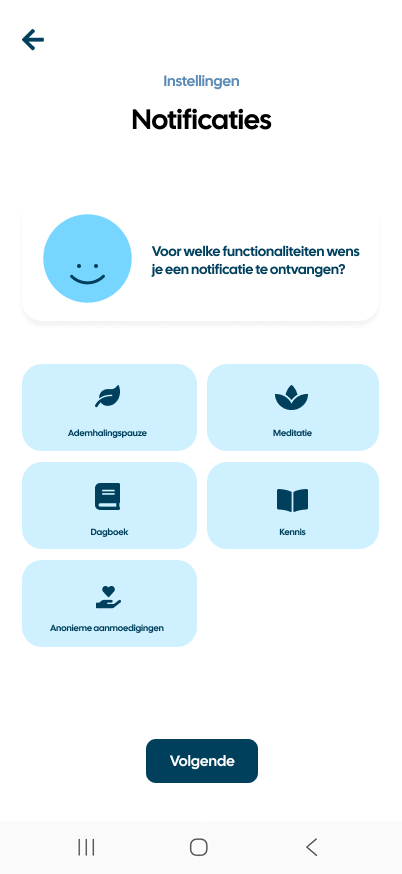
\includegraphics[width=\linewidth]{../graphics/Mockups/Onboarding/onboarding14}
    \end{minipage}
    \hfill
    \begin{minipage}{0.3\textwidth}
        \centering
        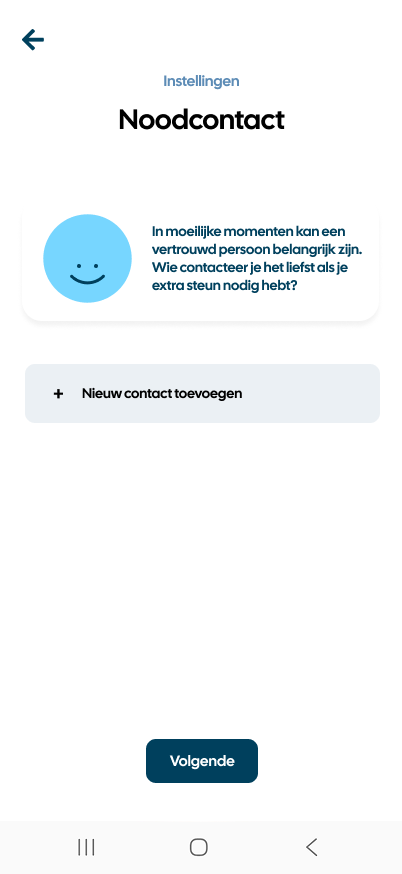
\includegraphics[width=\linewidth]{../graphics/Mockups/Onboarding/onboarding15}
    \end{minipage}
    \hfill
    \begin{minipage}{0.3\textwidth}
        \centering
        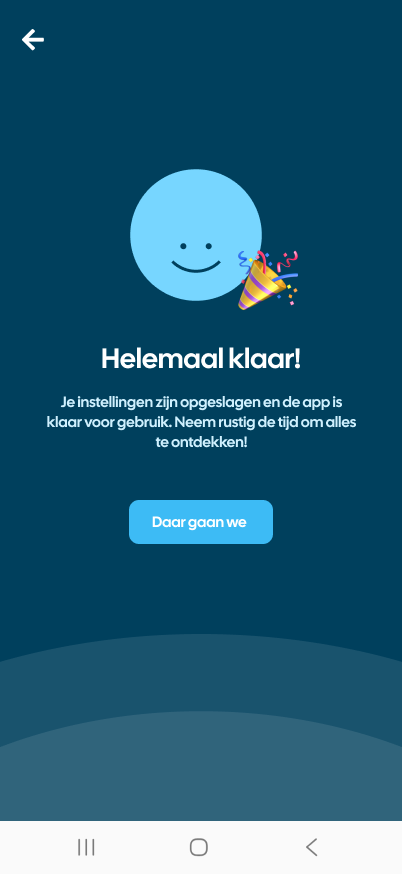
\includegraphics[width=\linewidth]{../graphics/Mockups/Onboarding/onboarding16}
    \end{minipage}
    
    \vspace{1em}
    
    \begin{minipage}{0.3\textwidth}
        \centering
        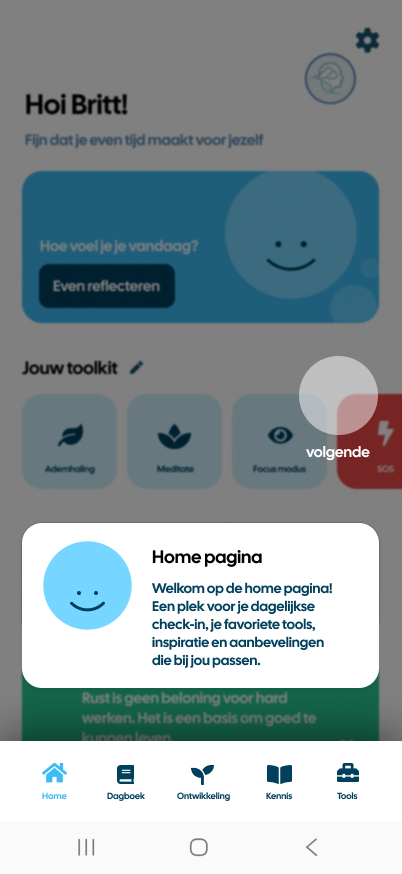
\includegraphics[width=\linewidth]{../graphics/Mockups/Onboarding/onboarding17}
    \end{minipage}
    \hfill
    \begin{minipage}{0.3\textwidth}
        \centering
        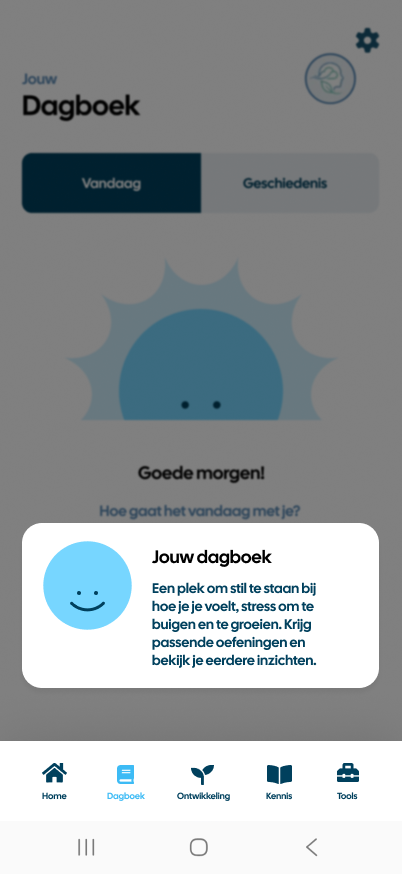
\includegraphics[width=\linewidth]{../graphics/Mockups/Onboarding/onboarding18}
    \end{minipage}
    \hfill
    \begin{minipage}{0.3\textwidth}
        \centering
        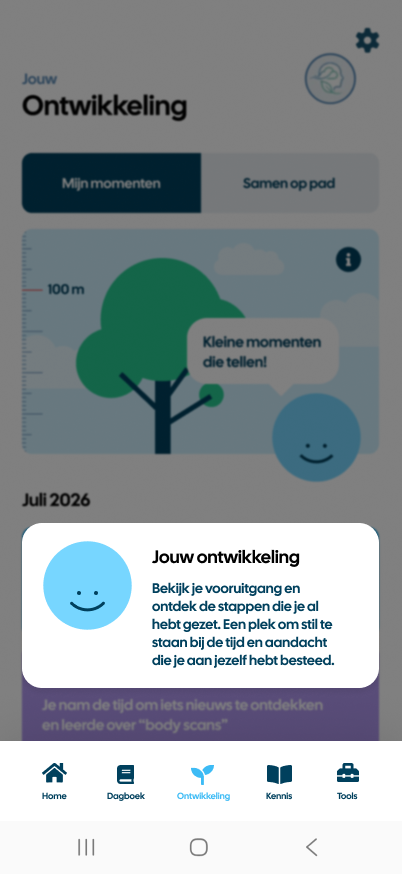
\includegraphics[width=\linewidth]{../graphics/Mockups/Onboarding/onboarding19}
    \end{minipage}
    
    \caption{Mockups van de verdere onboarding: notificatievoorkeuren, noodcontact, afronding en start van de rondleiding}
    \label{fig:mockups-16}
\end{figure}

\begin{figure}[H]
    \centering
    
    \begin{minipage}{0.3\textwidth}
        \centering
        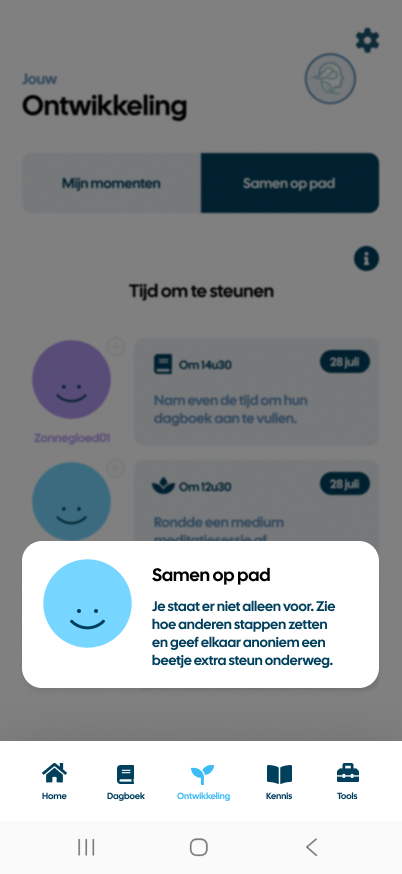
\includegraphics[width=\linewidth]{../graphics/Mockups/Onboarding/onboarding20}
    \end{minipage}
    \hfill
    \begin{minipage}{0.3\textwidth}
        \centering
        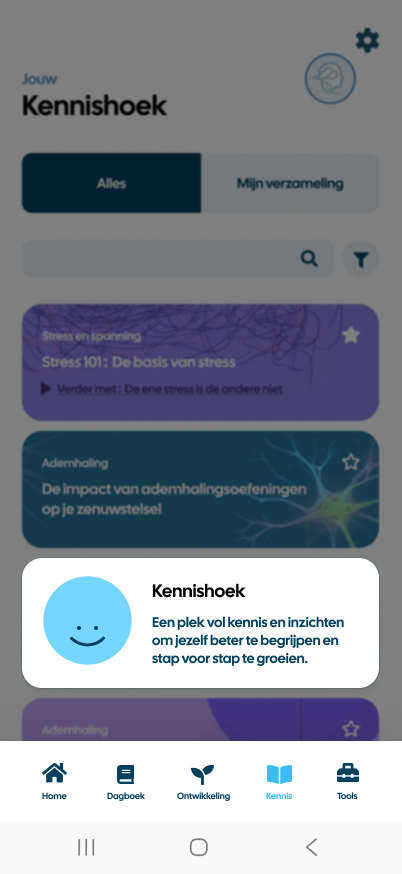
\includegraphics[width=\linewidth]{../graphics/Mockups/Onboarding/onboarding21}
    \end{minipage}
    \hfill
    \begin{minipage}{0.3\textwidth}
        \centering
        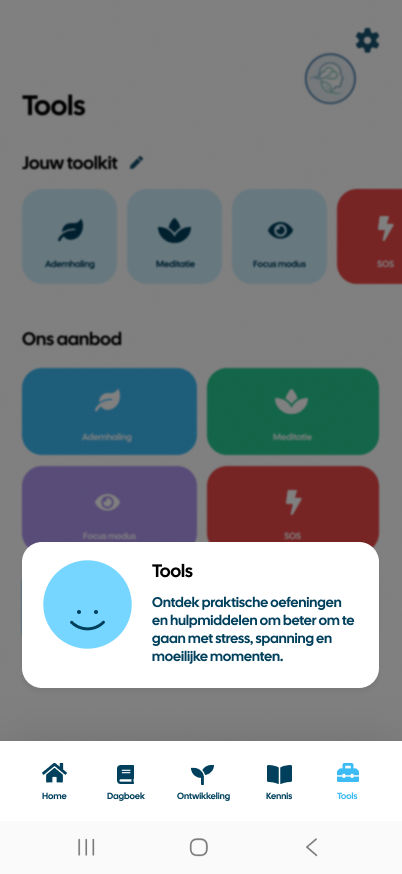
\includegraphics[width=\linewidth]{../graphics/Mockups/Onboarding/onboarding22}
    \end{minipage}
    
    \caption{Mockups van de rondleiding doorheen de applicatie}
    \label{fig:mockups-17}
\end{figure}

In de oorspronkelijke Burnout Free-app was geen onboarding aanwezig. Hierdoor werd de gebruiker bij het eerste gebruik niet begeleid bij het instellen van de applicatie en kreeg deze ook geen introductie tot de verschillende functionaliteiten. In de nieuwe versie werd daarom een onboarding toegevoegd die de gebruiker stap voor stap begeleidt bij het personaliseren van de applicatie en het instellen van de gewenste ondersteuning.

\vspace{1em}

{\small
    \begin{itemize}
        \item De gebruiker wordt bij de start geïnformeerd over de werking en beperkingen van de applicatie, waaronder de mogelijkheid om professionele hulp te raadplegen. Hierdoor worden verwachtingen duidelijk gemaakt zonder te suggereren dat de applicatie professionele hulp vervangt (\textbf{Ontwerpprincipe}: \textit{duidelijke positionering, ondersteunende communicatie, zichtbare meerwaarde}).
        
        \item Privacygevoelige keuzes, zoals het aanmaken van een account, het delen van gegevens met de community en andere toestemmingen, worden niet standaard geactiveerd. De gebruiker bepaalt zelf welke keuzes worden toegestaan, waardoor de controle over persoonlijke gegevens bij de gebruiker blijft (\textbf{Ontwerpprincipe}: \textit{Privacy by Design, ondersteun autonomie}).
        
        \item De verschillende instellingen worden stap voor stap bevraagd, waaronder naam, voorkeuren, gewenste ondersteuning, notificatiefrequentie en noodcontact. Door deze keuzes verspreid over meerdere schermen aan te bieden en in een conversatievorm te formuleren, wordt de hoeveelheid informatie per scherm beperkt (\textbf{Ontwerpprincipes}: \textit{minimaliseer cognitieve belasting, ondersteunende communicatie}).
        
        \item De gebruiker wordt op een laagdrempelige manier begeleid bij het instellen van notificaties en ondersteuning. Hierdoor worden persoonlijke voorkeuren meteen meegenomen in de verdere werking van de applicatie (\textbf{Ontwerpprincipes}: \textit{persoonlijke relevantie, ondersteun autonomie}).
        
        \item Na het instellen van de applicatie krijgt de gebruiker een korte rondleiding doorheen de belangrijkste pagina's. Hierbij wordt per pagina toegelicht welke functionaliteiten er beschikbaar zijn, zodat de gebruiker weet waar bepaalde mogelijkheden terug te vinden zijn (\textbf{Ontwerpprincipes}: \textit{techno-simplicity, ondersteun competentiegevoel}).
    \end{itemize}
}

\newpage

\section{Implementatie in code}
\label{sec:implementatie-code}

\vspace{1em}

Na de uitwerking van de mock-ups werd een selectie van de ontworpen schermen vertaald naar een werkende frontend-implementatie. Het doel hiervan is niet om binnen de scope van deze bachelorproef een applicatie te ontwikkelen die klaar is voor productie, maar om na te gaan in welke mate de voorgestelde functionaliteiten en ontwerpprincipes technisch realiseerbaar zijn. De implementatie vormt daarmee een technische verdieping van de eerder uitgewerkte mock-ups en maakt het mogelijk om niet enkel het visuele ontwerp, maar ook interacties en toestandsveranderingen af te toetsen.

\vspace{1em}

Zoals eerder gemotiveerd werd in sectie \ref{sec:app-tech-keuze}, werd deze implementatie uitgevoerd met React Native, specifieker met het Expo-framework. Er werden onder andere een splashscreen, startpagina, toolkit, profielpagina, instellingen, dagboek, meditatieoefening en bijhorende interacties uitgewerkt. Gegevens die in een volwaardige applicatie vanuit een backend of database zouden worden opgehaald, worden binnen deze \acrshort{poc} gesimuleerd aan de hand van mock data. Hierdoor kunnen de belangrijkste gebruikersinteracties worden gedemonstreerd zonder dat een volledige backendarchitectuur noodzakelijk is.

\vspace{1em}

De implementatie omvat bewust niet alle schermen en functionaliteiten die in de mock-ups werden uitgewerkt. Gezien de omvang van de voorgestelde applicatie werd een gerichte selectie gemaakt van schermen en interacties die representatief zijn voor de verschillende ontwerpprincipes en functionaliteiten. Op die manier kan binnen de beschikbare scope worden nagegaan of de belangrijkste ontwerpkeuzes technisch realiseerbaar zijn, zonder dat de volledige applicatie moet worden geïmplementeerd. De niet-geïmplementeerde schermen blijven hierdoor onderdeel van het voorgestelde ontwerp, maar vallen buiten de technische uitwerking van deze \acrshort{poc}.

\vspace{1em}

\subsubsection{Personalisatie en begeleidingsintensiteit}
\label{sec:personalisatie-code}

\vspace{1em}

De begeleidingsintensiteit werd binnen de \acrshort{poc} niet enkel als een visuele instelling uitgewerkt, maar heeft ook invloed op het gedrag van de applicatie. De gebruiker kan aangeven hoeveel begeleiding gewenst is en in welke mate herinneringen gewenst zijn. Op basis van deze keuzes wordt bepaald welke vormen van ondersteuning worden aanbevolen, hoeveel herinneringen worden voorzien en op welke momenten deze plaatsvinden. Deze logica wordt in de implementatie vertaald naar een profiel dat wordt bepaald op basis van de gekozen instellingen. Hiervoor worden de verschillende waarden gecombineerd tot een unieke sleutel, waarmee het overeenkomstige profiel uit de mock data kan worden opgehaald.

\vspace{1em}

\begin{listing}[H]
    \begin{minted}{typescript}
        const profileKey = `${supportLevel}_${reminderNeed}`;
        const notificationProfile = notificationProfiles[profileKey];
    \end{minted}
    \caption[Selecteren van een personalisatieprofiel]
    {Selecteren van het personalisatieprofiel op basis van gebruikersvoorkeuren.}
    \label{lst:profile-selection}
\end{listing}

\vspace{1em}

Het geselecteerde profiel bevat vervolgens de instellingen voor de verschillende vormen van ondersteuning. Een wijziging van de begeleidingsintensiteit kan hierdoor bijvoorbeeld leiden tot een andere frequentie van herinneringen of tot andere aanbevolen functies.

\vspace{1em}

\begin{listing}[H]
    \begin{minted}{typescript}
        const notificationProfiles: Record<string, NotificationProfile> = {
            
            // LOW: weinig begeleiding
            low_low: { 
                journal: [], 
                breathing: [{ hour: 14 }], 
                meditation: [] 
            },
            
            // MEDIUM: balans
            medium_medium: { 
                journal: [{ hour: 9 }], 
                breathing: [{ hour: 14 }], 
                meditation: [{ hour: 19 }] 
            },
            
            // HIGH: intensieve begeleiding
            high_high: {
                journal: [{ hour: 9 }],
                breathing: [{ hour: 9 }, { hour: 14 }, { hour: 19 }],
                meditation: [{ hour: 9 }, { hour: 19 }]
            }
        };
    \end{minted}
    \caption[Vooraf gedefinieerde notificatieprofielen]
    {Vooraf gedefinieerde notificatieprofielen met verschillende ondersteuningsintensiteiten.}
    \label{lst:notification-profiles}
\end{listing}

\begin{listing}[H]
    \begin{minted}[escapeinside=||]{typescript}
        const RECOMMENDED_MEDITATION_DURATION: Record<SupportLevel, number> = {
            low: 3,
            medium: 5,
            high: 10,
        };
        
        const isRecommended = durationOption.value === recommendedDuration;
        
        return (
        <View key={durationOption.value} style={styles.optionWrapper}>
        {isRecommended && (
            <View style={styles.recommendedLabel}>
                <Text style={styles.recommendedLabelText}>Mijn aanrader|\texttt{</Text>}|
                <Image
                    source={require('@/assets/images/Coach_Bubbles.png')}
                    style={styles.recommendedCoach}
                    resizeMode="contain"
                />
            |\texttt{</View>}|
            )}
    \end{minted}
    \caption[Aanbevolen meditatieduur]
    {Aanbevolen meditatieduur afgestemd op de gekozen begeleidingsintensiteit.}
    \label{lst:recommended-meditation-duration}
\end{listing}

\vspace{1em}

Hiermee wordt het principe van \textit{Persoonlijke autonomie en keuzevrijheid} concreet toegepast. De gebruiker bepaalt zelf de gewenste begeleidingsintensiteit, waarna de applicatie de aangeboden ondersteuning hierop afstemt. Tegelijkertijd wordt het principe \textit{Beperk digitale interrupties} ondersteund, aangezien de hoeveelheid en timing van herinneringen afhankelijk zijn van de persoonlijke voorkeuren van de gebruiker.

\vspace{1em}

Binnen deze \acrshort{poc} wordt hiervoor gewerkt met vooraf gedefinieerde profielen en worden de notificaties niet daadwerkelijk als pushnotificaties verstuurd. De implementatie toont wel aan dat een wijziging van gebruikersvoorkeuren kan worden vertaald naar een wijziging in het gedrag en de aangeboden ondersteuning van de applicatie.

\newpage

\subsubsection{Inclusieve toegankelijkheid}
\label{sec:toegankelijkheid-code}

\vspace{1em}

Ook het \textit{Inclusieve toegankelijkheid} ontwerpprincipe werd meegenomen in de technische implementatie. Hierbij werd niet uitsluitend rekening gehouden met de visuele interface, maar ook met de manier waarop interactieve elementen door verschillende gebruikers kunnen worden bediend.

\vspace{1em}

Een voorbeeld hiervan is de knop waarmee de instellingen worden geopend:

\begin{listing}[H]
    \begin{minted}[escapeinside=||]{typescript}
        <Pressable
            onPress={() => setSettingsVisible(true)}
            accessibilityRole="button"
            accessibilityLabel="Instellingen openen"
            hitSlop={8}
        >
            <IconSymbol
            size={25}
            name="gear.fill"
            color={colors.darkBlue}
            />
        |\texttt{</Pressable>}|
    \end{minted}
    \caption[Toegankelijke instellingenknop]
    {Toegankelijk geïmplementeerde instellingenknop met semantische rol, toegankelijkheidslabel en vergroot aanraakgebied.}
    \label{lst:accessible-settings-button}
\end{listing}

Het attribuut \texttt{accessibilityRole} maakt duidelijk dat het element een knop is, terwijl \texttt{accessibilityLabel} een beschrijving voorziet voor gebruikers van ondersteunende technologie, zoals een screenreader. Daarnaast vergroot \texttt{hitSlop} het effectieve aanraakgebied van de knop zonder de visuele grootte ervan te wijzigen. Dit maakt de interactie minder afhankelijk van het exact raken van het icoon en ondersteunt daarmee een meer inclusieve bediening.

\newpage

\subsubsection{Cross-platform en distributie}
\label{sec:cross-platform-code}

\vspace{1em}

Het cross-platform karakter van React Native werd tijdens de implementatie onder andere meegenomen in de manier waarop iconen worden weergegeven. Hiervoor werd een eigen \texttt{IconSymbol}-component voorzien die een abstracte iconnaam koppelt aan een concrete iconimplementatie.

\begin{listing}[H]
    \begin{minted}{typescript}
        const MAPPING = {
            'house.fill': 'house-chimney',
            'journal.fill': 'book',
            'toolbox.fill': 'toolbox',
            'gear.fill': 'gear',
            'bell.fill': 'bell',
            'user.fill': 'user-large',
            'play': 'play',
            ...
        };
    \end{minted}
    \caption[Centraal beheerde iconmapping]
    {Centrale mapping waarbij abstracte iconnamen worden gekoppeld aan concrete iconimplementaties.}
    \label{lst:icon-mapping}
\end{listing}

De schermen maken hierdoor gebruik van eenzelfde abstracte benaming, terwijl de concrete iconimplementatie centraal wordt beheerd. De gebruikte structuur maakt het bovendien mogelijk om indien nodig verschillende iconen per platform te voorzien, zonder de schermen zelf hiervoor aan te passen. Dit ondersteunt het ontwerpprincipe \textit{Snel en eenvoudig distribueerbaar}. De applicatie kan vanuit één codebasis voor verschillende mobiele platformen worden ontwikkeld, terwijl platformafhankelijke implementatiedetails op een centrale plaats kunnen worden opgevangen. Binnen de huidige \acrshort{poc} werden de iconen nog niet visueel per platform aangepast, maar de gekozen structuur laat deze uitbreiding wel toe.

\newpage

\subsubsection{Foutafhandeling meldingrechten}
\label{sec:foutafhandeling-code}

\vspace{1em}

In de oorspronkelijke applicatie werd bij het weigeren van notificatierechten een technische foutmelding \texttt{ns\_denied} weergegeven (zie \ref{fig:burnout-free-6}). Dit gaf de gebruiker weinig informatie over het probleem. Dit werd in de PoC opgelost door de notificatierechten expliciet te controleren en fouten af te handelen.

Met behulp van \texttt{expo-notifications} wordt eerst nagegaan of de applicatie toestemming heeft om notificaties te versturen. Indien nodig wordt de gebruiker om toestemming gevraagd. 

\begin{listing}[H]
    \begin{minted}{typescript}
        const currentPermissions = await Notifications.getPermissionsAsync();
        
        const permissions = currentPermissions.granted
        ? currentPermissions
        : await Notifications.requestPermissionsAsync();
        
        return (
            permissions.granted ||
            permissions.ios?.status === Notifications.IosAuthorizationStatus.PROVISIONAL
        );
    \end{minted}
    \caption[Controleren en aanvragen van notificatierechten]
    {Controleren en indien nodig aanvragen van notificatierechten voor notificaties.}
    \label{lst:melding-toestemming}
\end{listing}

Wanneer het controleren of aanvragen van de rechten mislukt, wordt de fout intern opgevangen. Wanneer notificaties vervolgens niet kunnen worden ingepland, worden de bijhorende toggles uitgeschakeld en krijgt de gebruiker een duidelijke melding met een mogelijke oplossing. Deze aanpak vervangt de oorspronkelijke technische foutmelding door een begrijpelijke gebruikersmelding en zorgt ervoor dat de applicatie ook zonder notificaties verder gebruikt kan worden.

\begin{listing}[H]
    \begin{minted}{typescript}
        try {
            // controleren en aanvragen van notificatierechten
        } catch (error) {
            console.warn('Notificaties zijn niet beschikbaar.', error);
            return false;
        }
    \end{minted}
    \caption[Afhandelen van fouten bij notificatierechten]
    {Intern opvangen van fouten bij het controleren of aanvragen van notificatierechten.}
    \label{lst:melding-error}
\end{listing}

\begin{listing}[H]
    \begin{minted}{typescript}
        if (!scheduled) {
            setAnonSupportEnabled(false);
            setJournalEnabled(false);
            setBreathingEnabled(false);
            setMeditationEnabled(false);
            
            Alert.alert(
                'Notificaties niet beschikbaar',
                'Geef BurnoutFree toestemming in de instellingen van je gsm. Je kan de app verder blijven gebruiken zonder notificaties.',
            );
        }
    \end{minted}
    \caption[Uitschakelen van notificatie-instellingen bij fouten]
    {Uitschakelen van notificatie-instellingen en tonen van een duidelijke melding wanneer notificaties niet beschikbaar zijn.}
    \label{lst:melding-alert}
\end{listing}

\vspace{1em}

\subsubsection{i18n}
\label{sec:i18n-code}

\vspace{1em}

In de \acrshort{poc} werd ook aandacht besteed aan het beperken van onnodige interactiestappen. Zo ondersteunt de \acrshort{poc} zowel Nederlands als Engels, waarbij de taal automatisch wordt bepaald op basis van de systeemtaal van het toestel. Hiervoor wordt de Expo-bibliotheek \texttt{expo-localization} gebruikt. Indien de systeemtaal niet wordt herkend als Engels, wordt Nederlands als standaardtaal gebruikt. Hierdoor hoeft de gebruiker tijdens de onboarding geen afzonderlijke taalkeuze te maken.

\begin{listing}[H]
    \begin{minted}{typescript}
        function getSystemLanguage(): Language {
            return getLocales()[0]?.languageCode === 'en' ? 'en' : 'nl';
        }
    \end{minted}
    \caption[Automatische selectie van de systeemtaal]
    {Automatische selectie van de applicatietaal op basis van de systeemtaal van het toestel.}
    \label{lst:i18n}
\end{listing}

Deze aanpak vermindert een extra keuzestap en sluit daarmee aan bij het principe om de interactielast voor de gebruiker zo laag mogelijk te houden.

\newpage

\subsubsection{Screenshots}
\label{sec:screenshots-code}

\begin{figure}[H]
    \centering
    
    \begin{minipage}{0.3\textwidth}
        \centering
        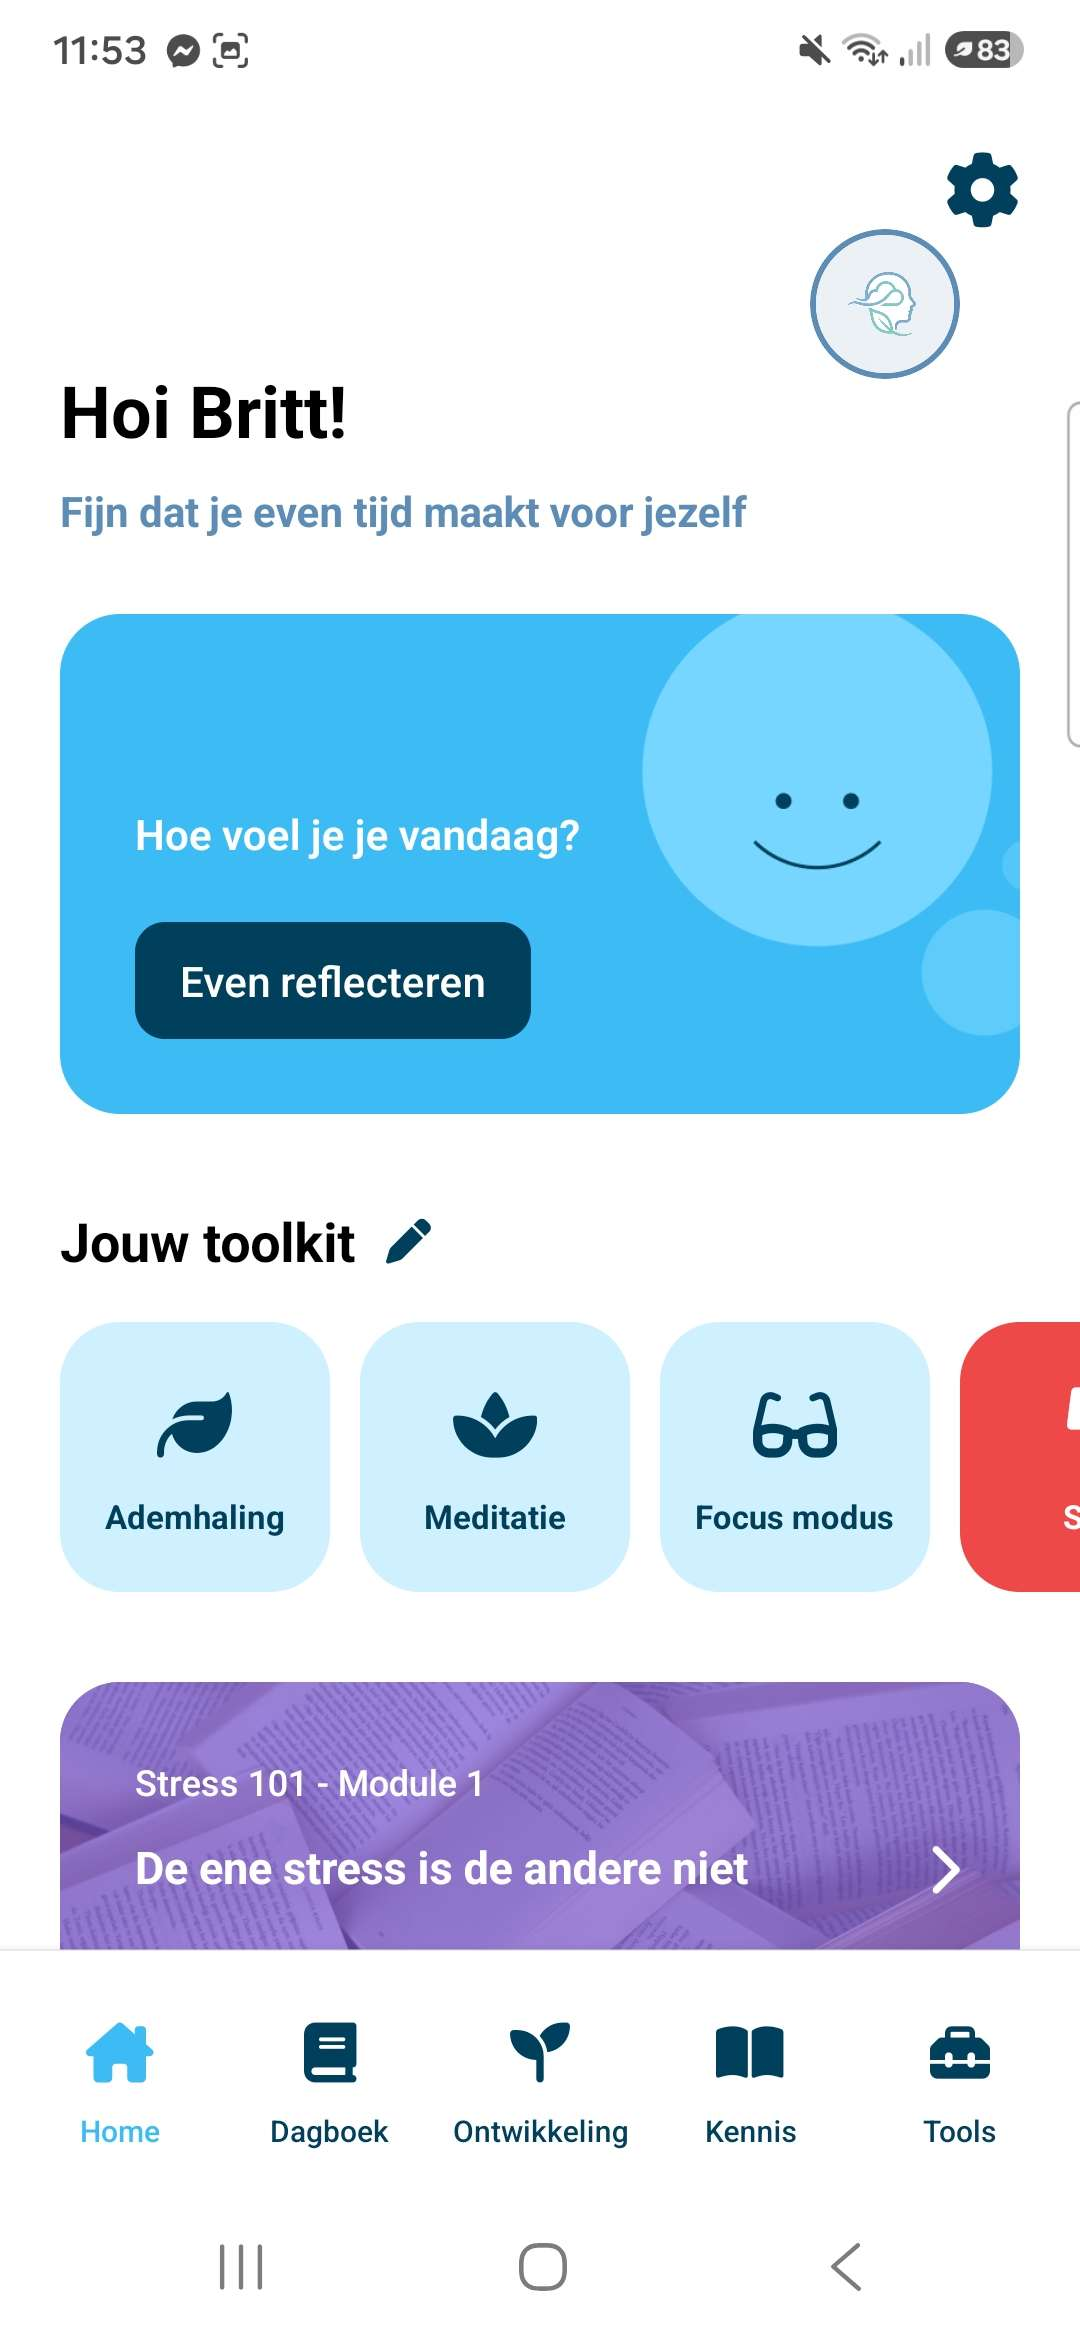
\includegraphics[width=\linewidth]{../graphics/Code/PoC1}
    \end{minipage}
    \hfill
    \begin{minipage}{0.3\textwidth}
        \centering
        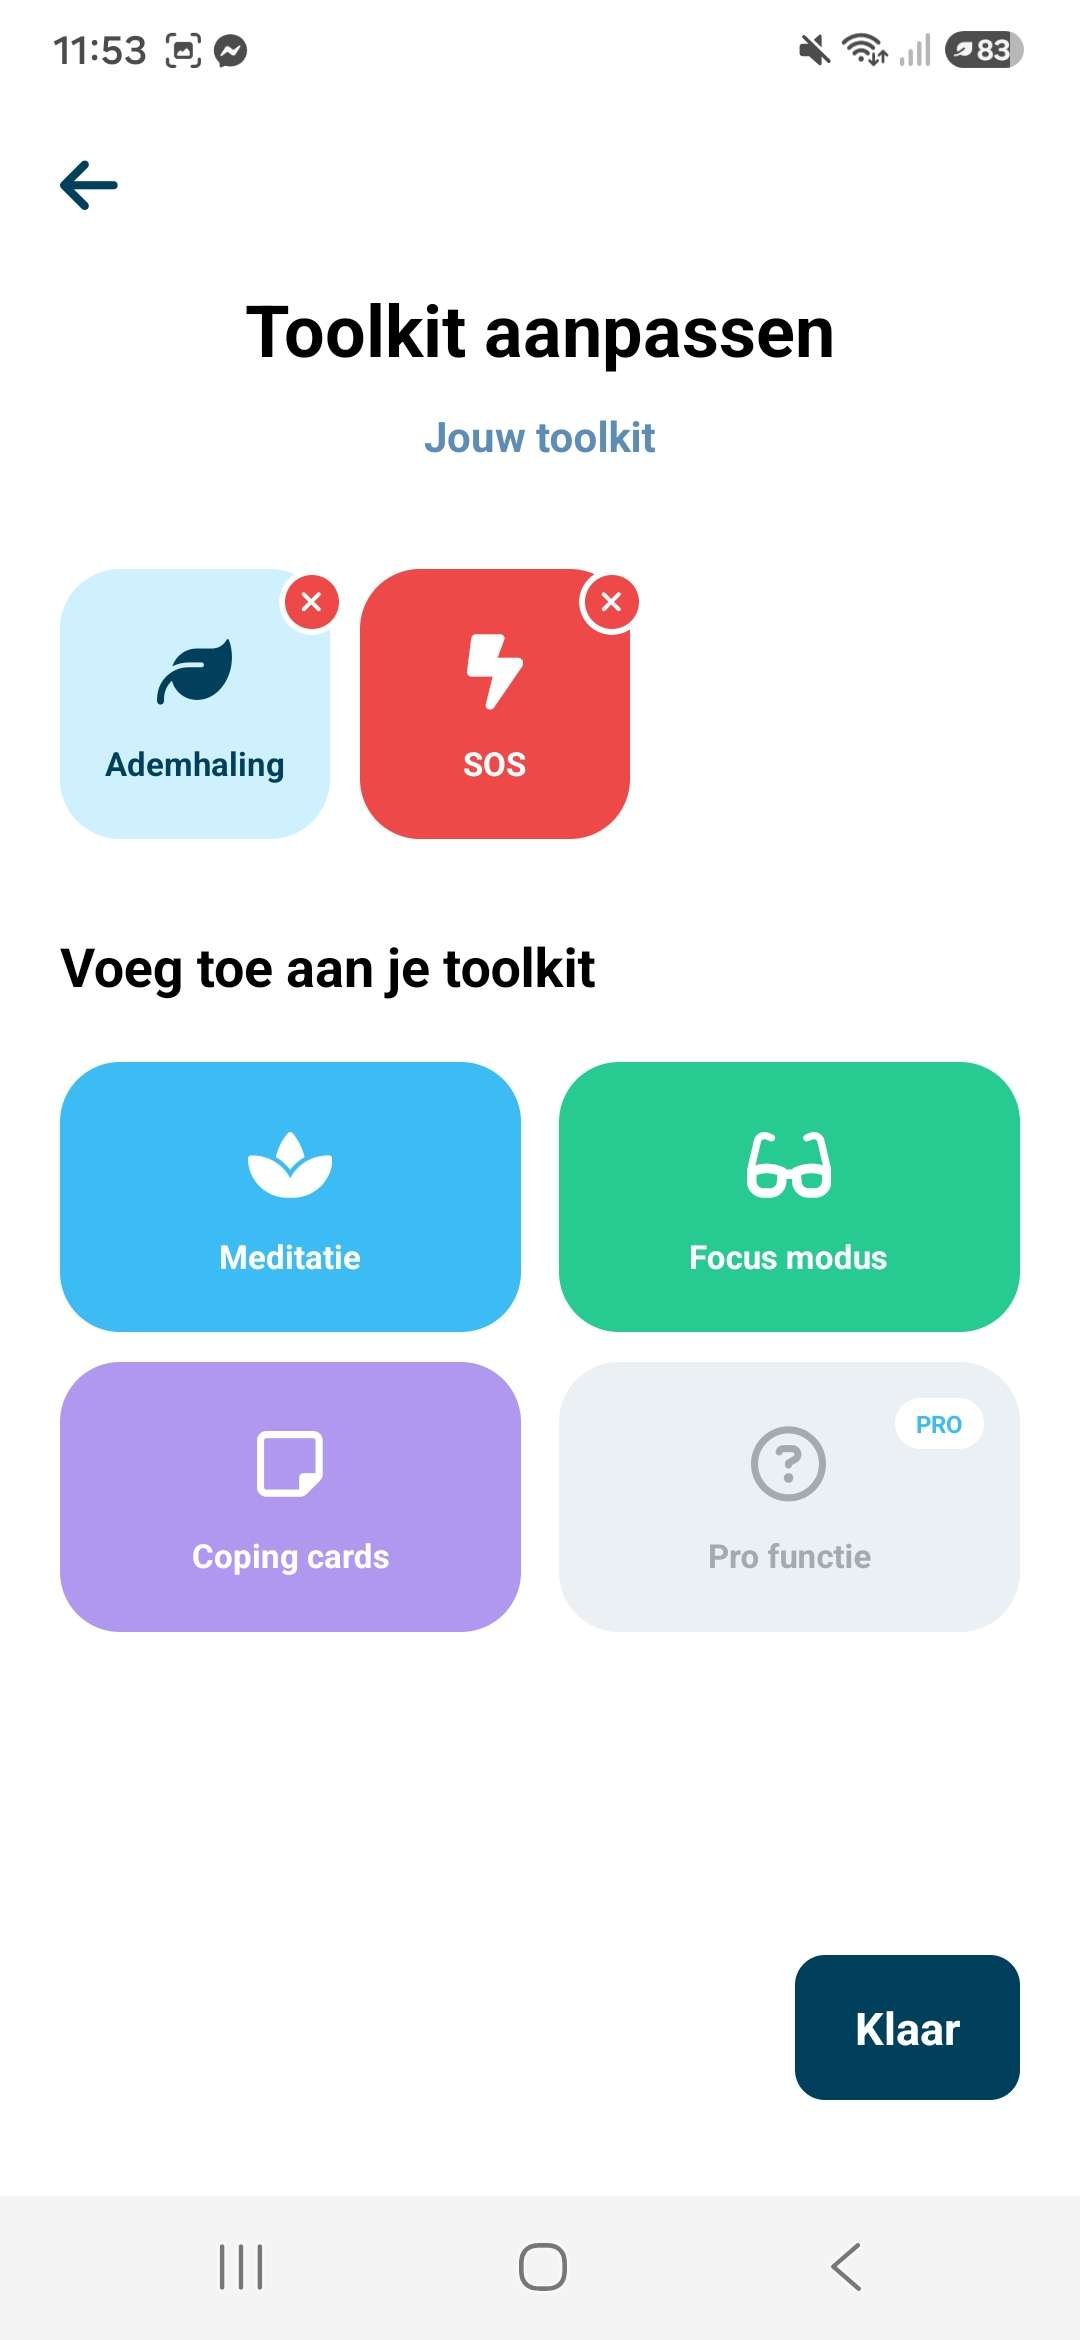
\includegraphics[width=\linewidth]{../graphics/Code/PoC2}
    \end{minipage}
    \hfill
    \begin{minipage}{0.3\textwidth}
        \centering
        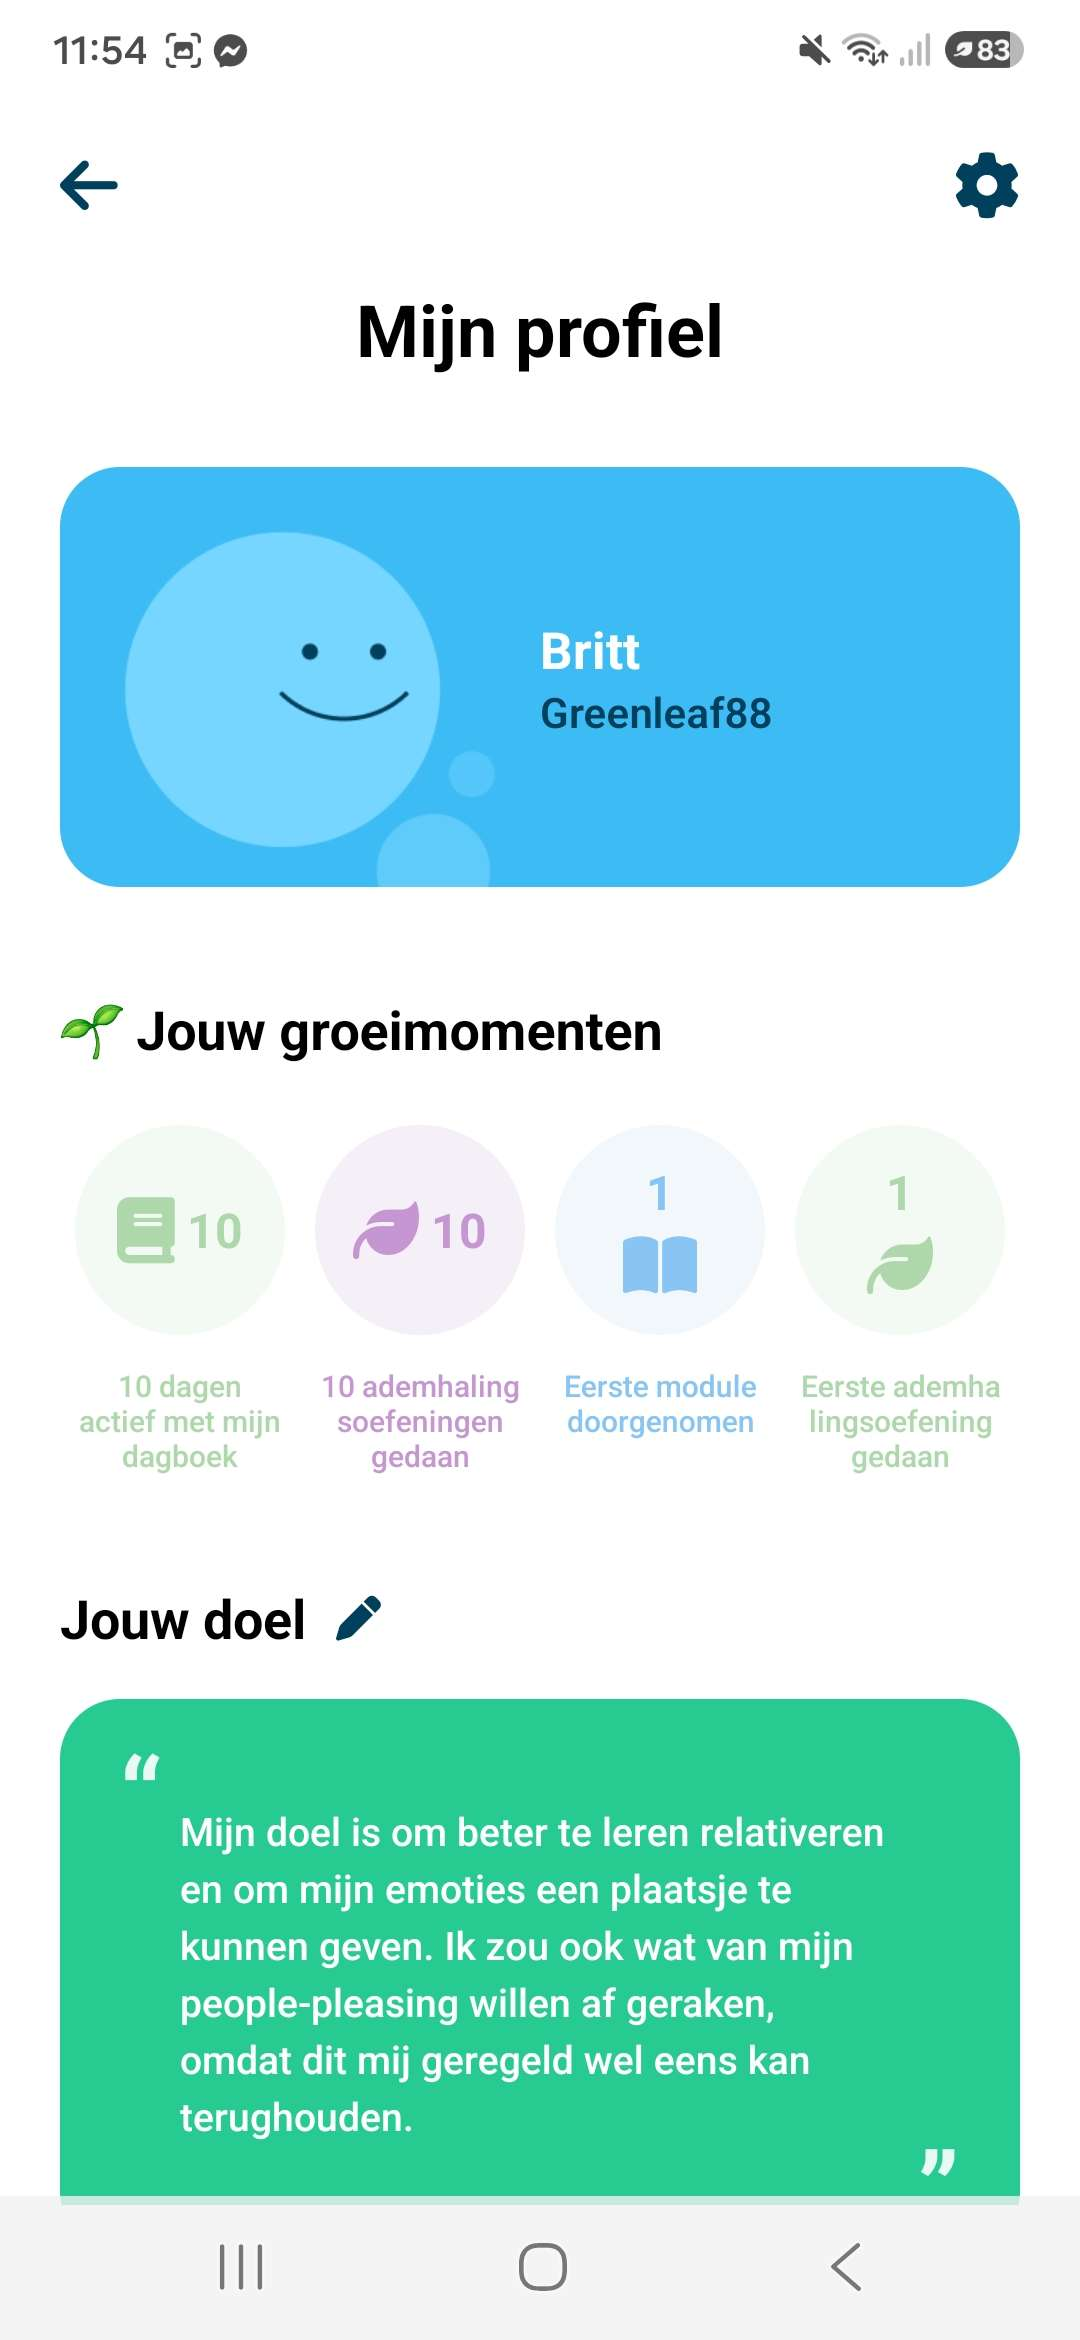
\includegraphics[width=\linewidth]{../graphics/Code/PoC3}
    \end{minipage}
    
    \vspace{1em}
    
    \begin{minipage}{0.3\textwidth}
        \centering
        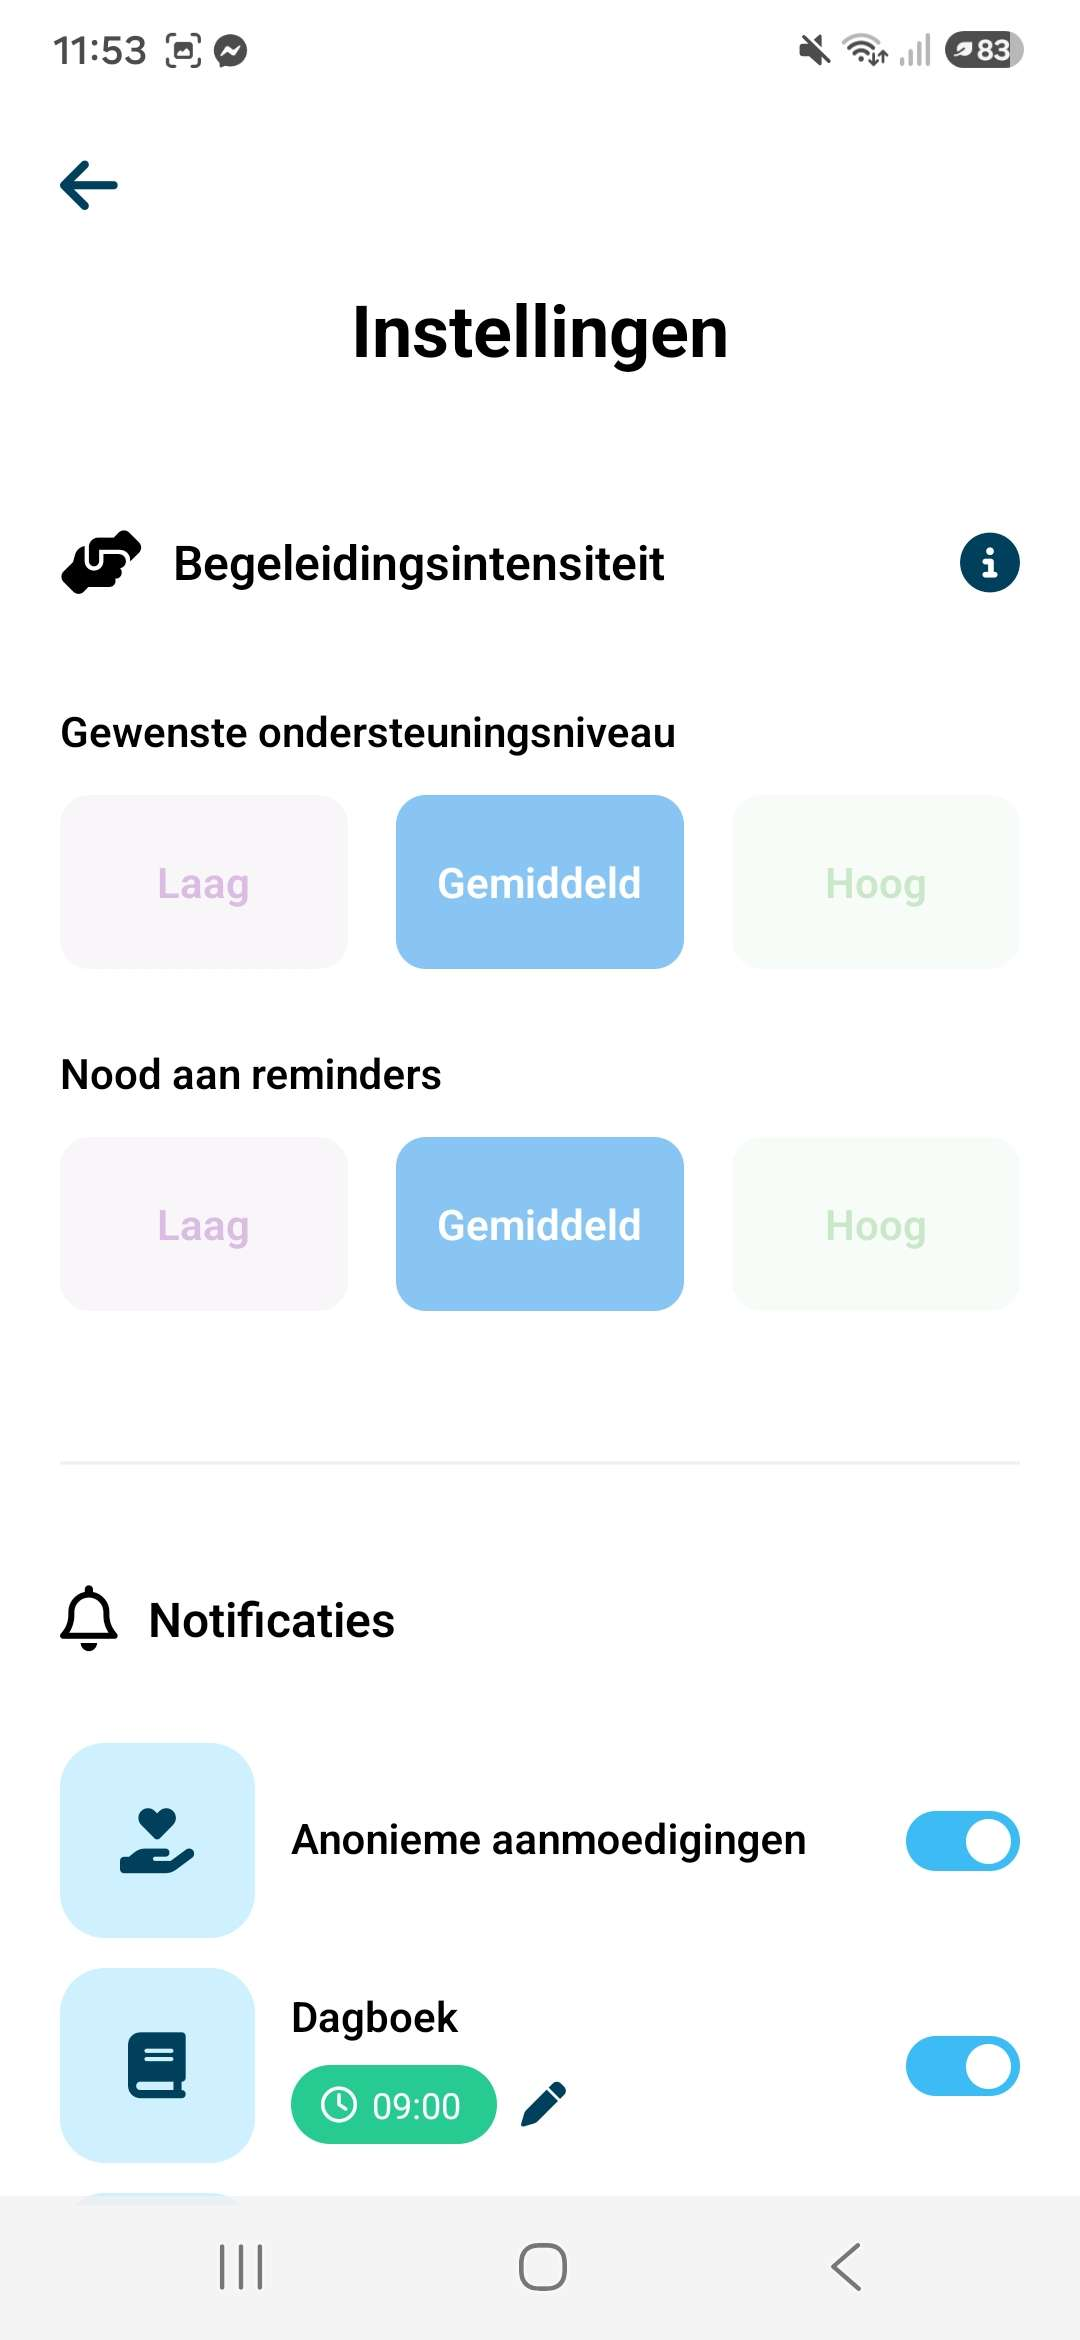
\includegraphics[width=\linewidth]{../graphics/Code/PoC4}
    \end{minipage}
    \hfill
    \begin{minipage}{0.3\textwidth}
        \centering
        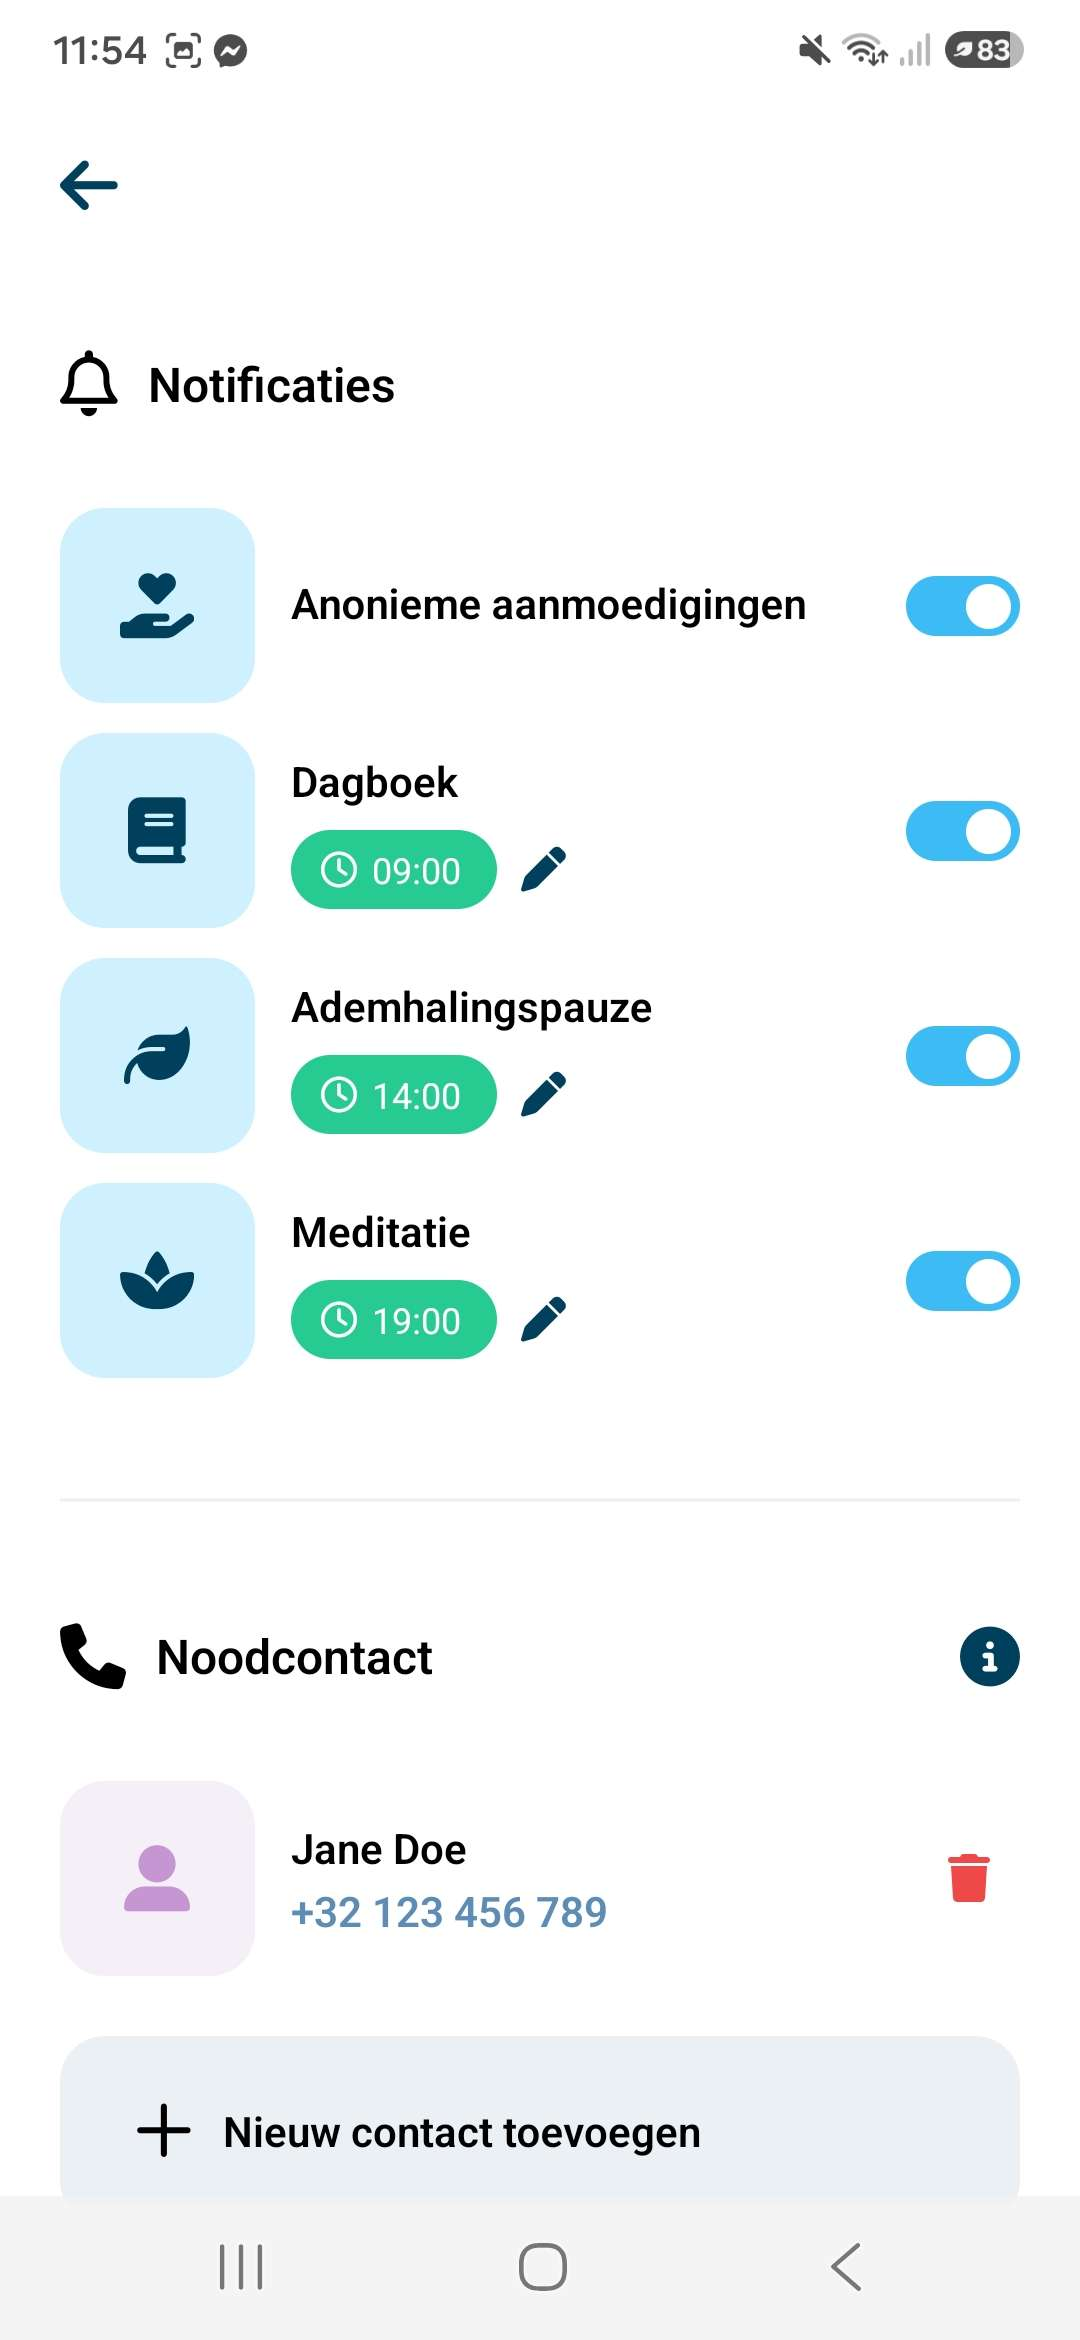
\includegraphics[width=\linewidth]{../graphics/Code/PoC5}
    \end{minipage}
    \hfill
    \begin{minipage}{0.3\textwidth}
        \centering
        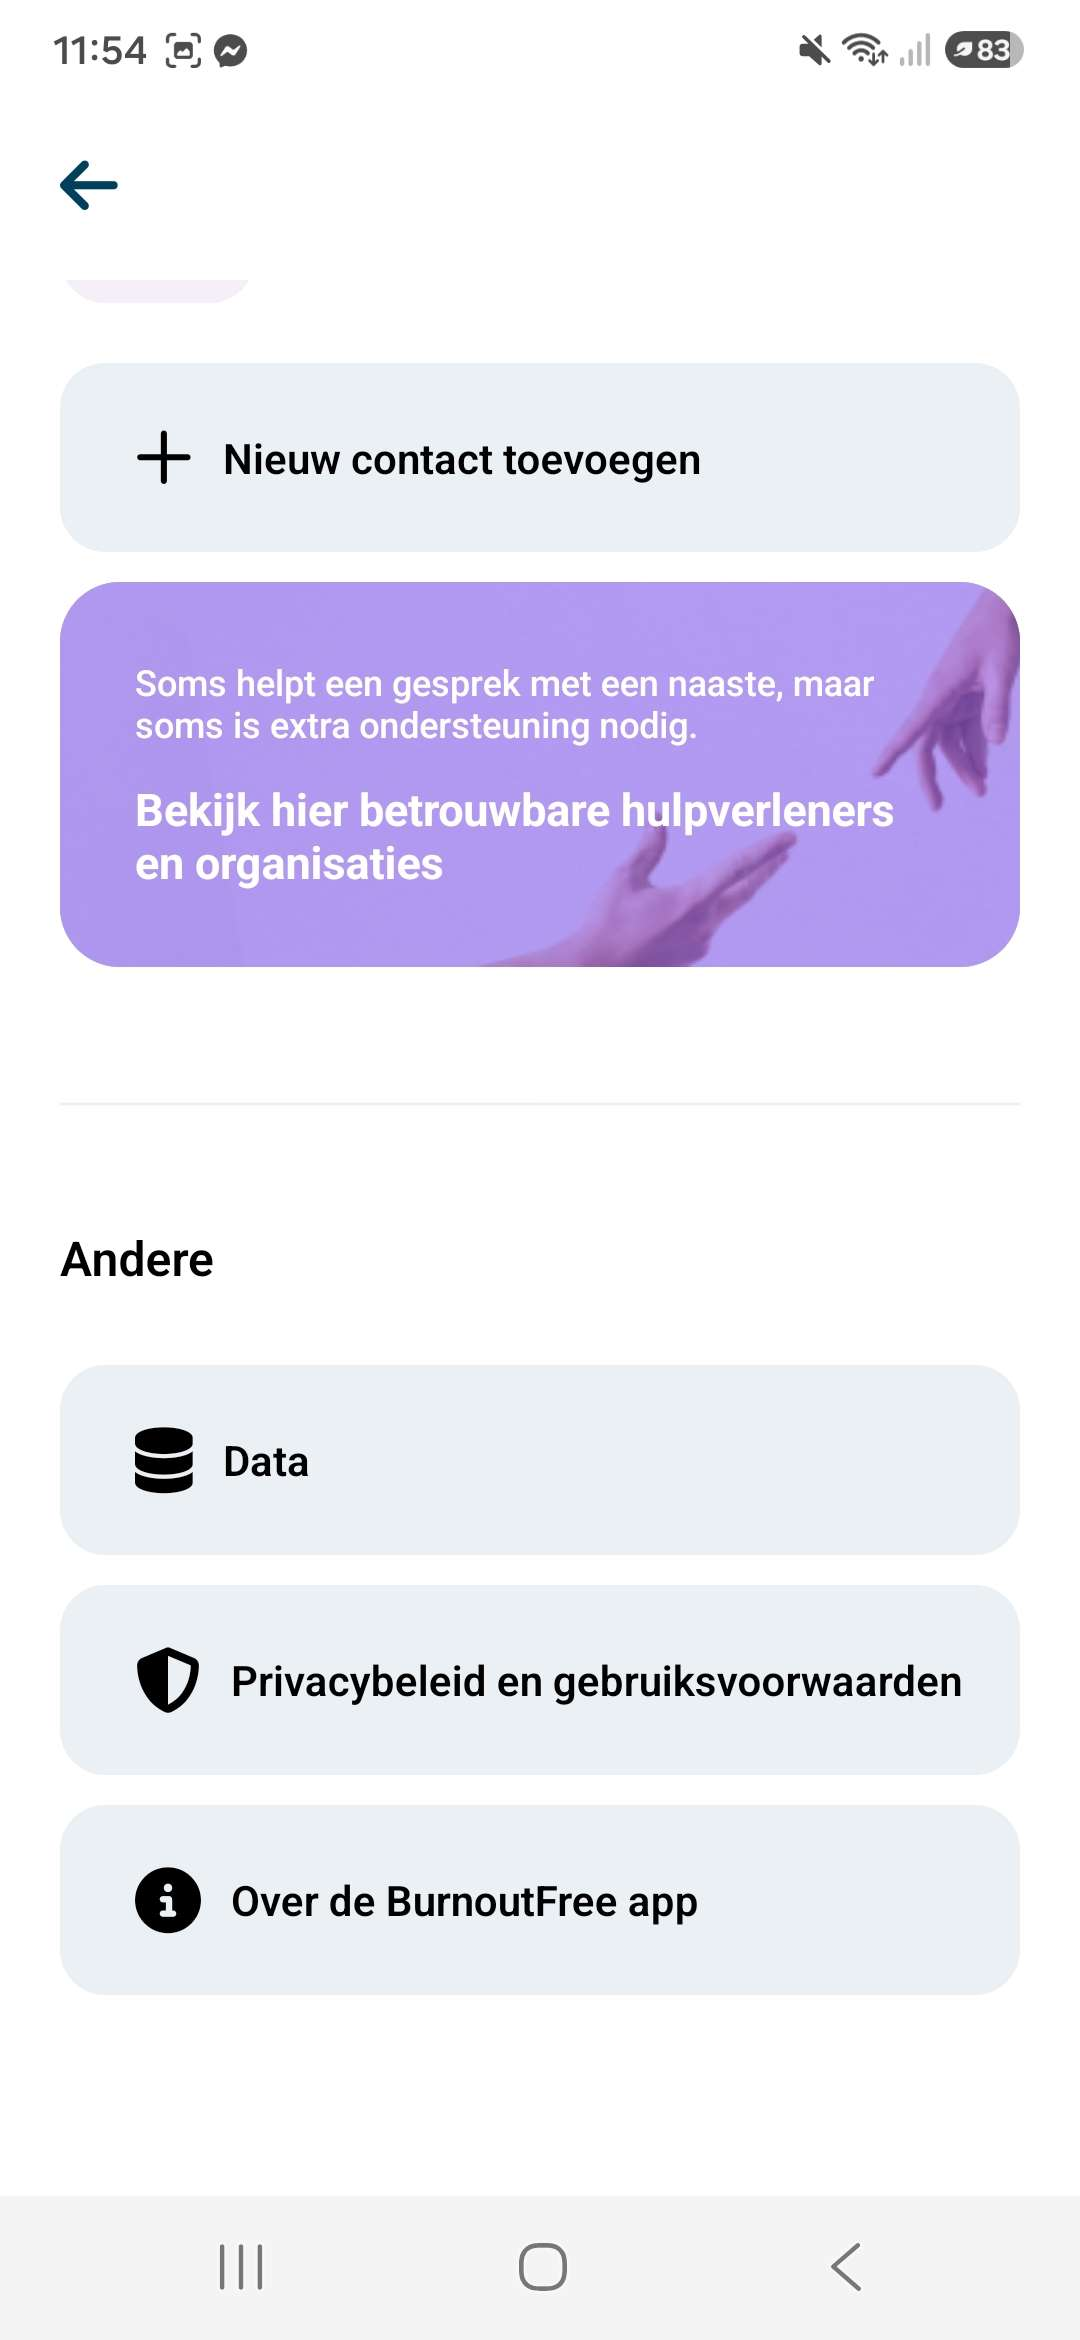
\includegraphics[width=\linewidth]{../graphics/Code/PoC6}
    \end{minipage}
    
    \caption{Overzicht van de belangrijkste schermen van de applicatie, waaronder de homepagina, toolkit, profielpagina en instellingen.}
    \label{fig:code-ss-1}
\end{figure}

\begin{figure}[H]
    \centering
    
    \begin{minipage}{0.3\textwidth}
        \centering
        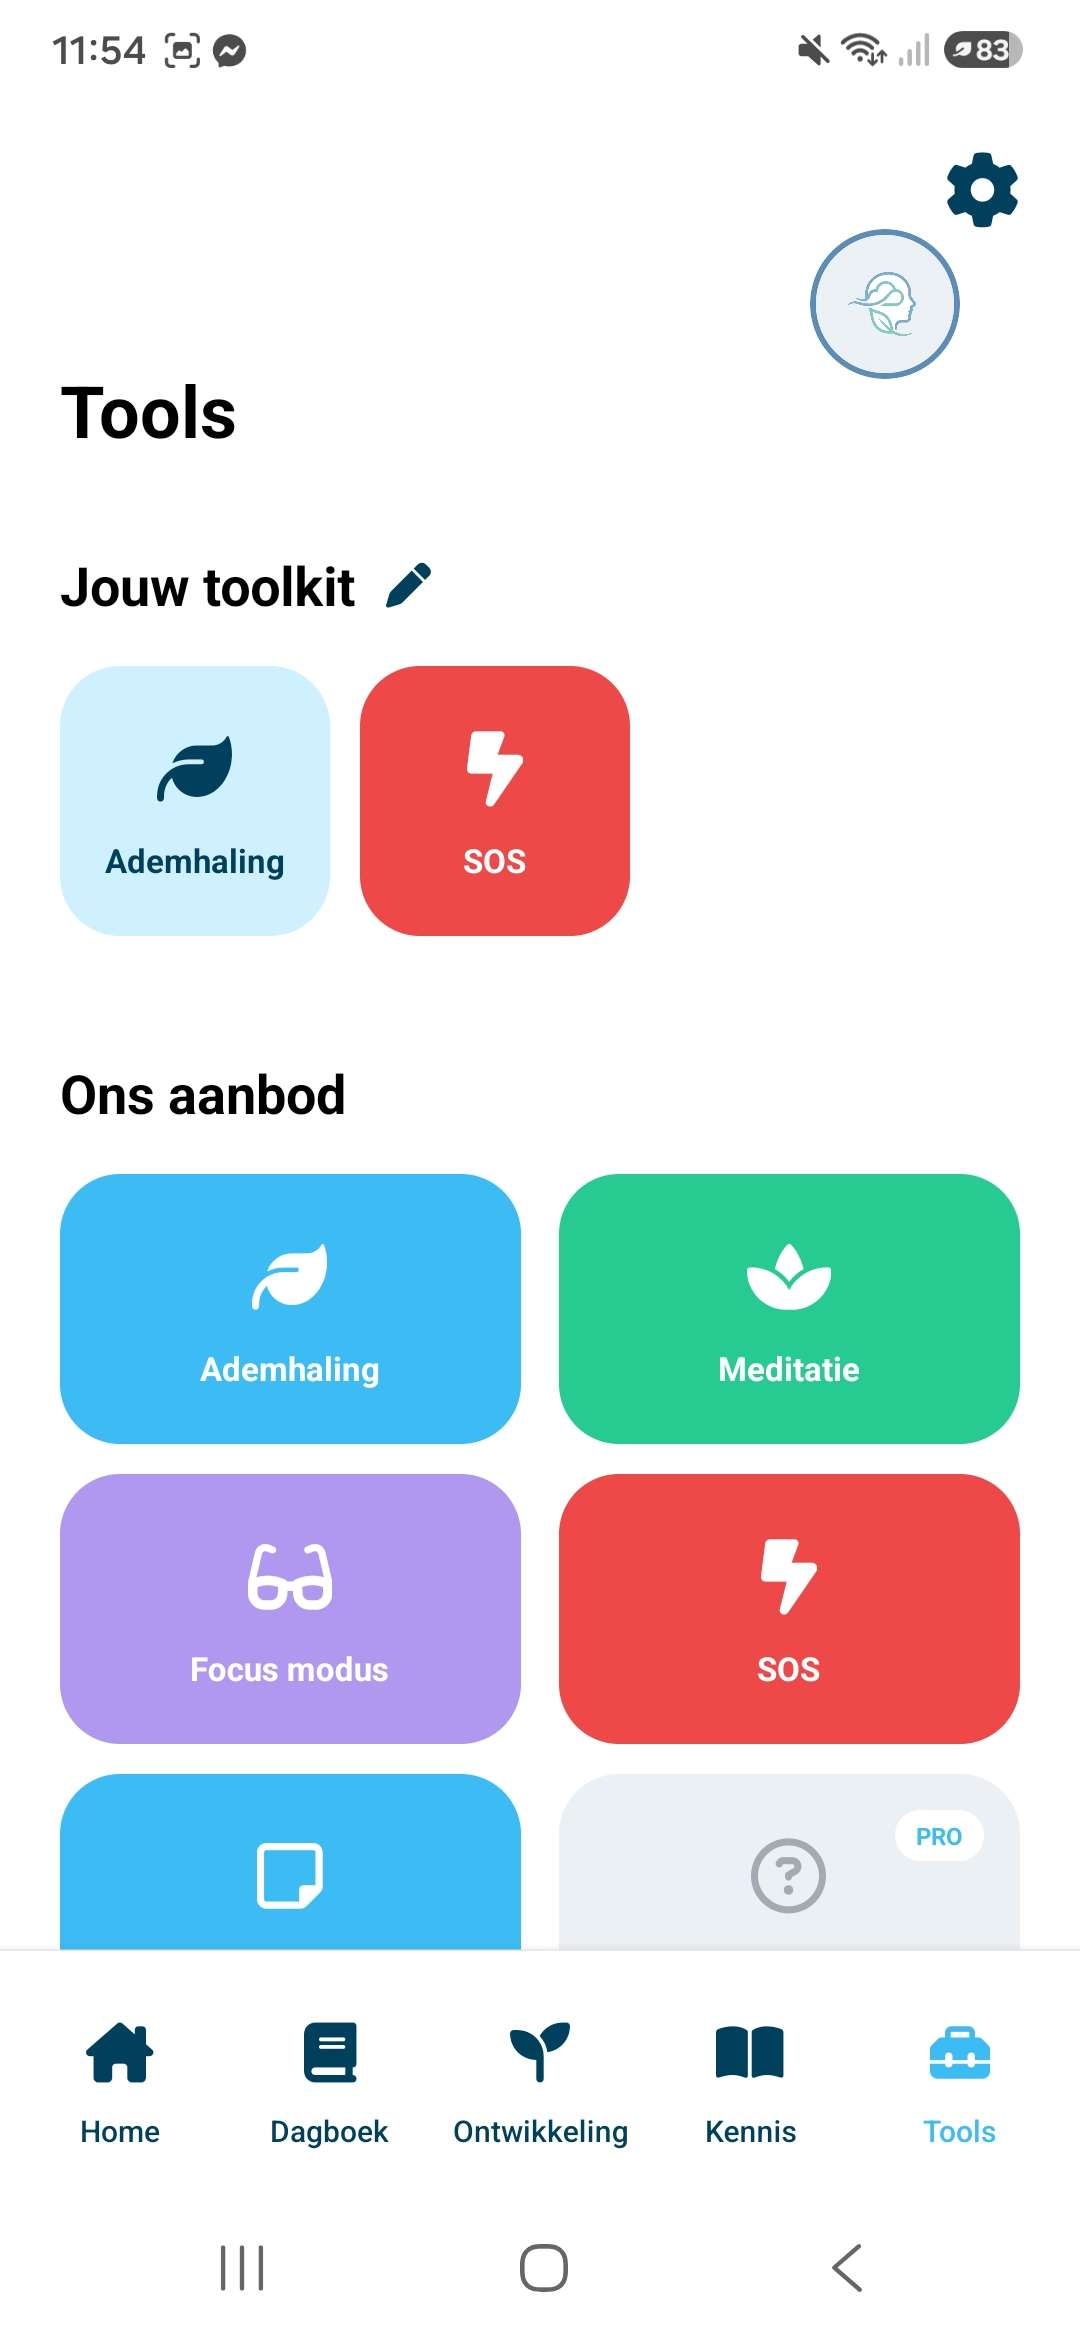
\includegraphics[width=\linewidth]{../graphics/Code/PoC7}
    \end{minipage}
    \hfill
    \begin{minipage}{0.3\textwidth}
        \centering
        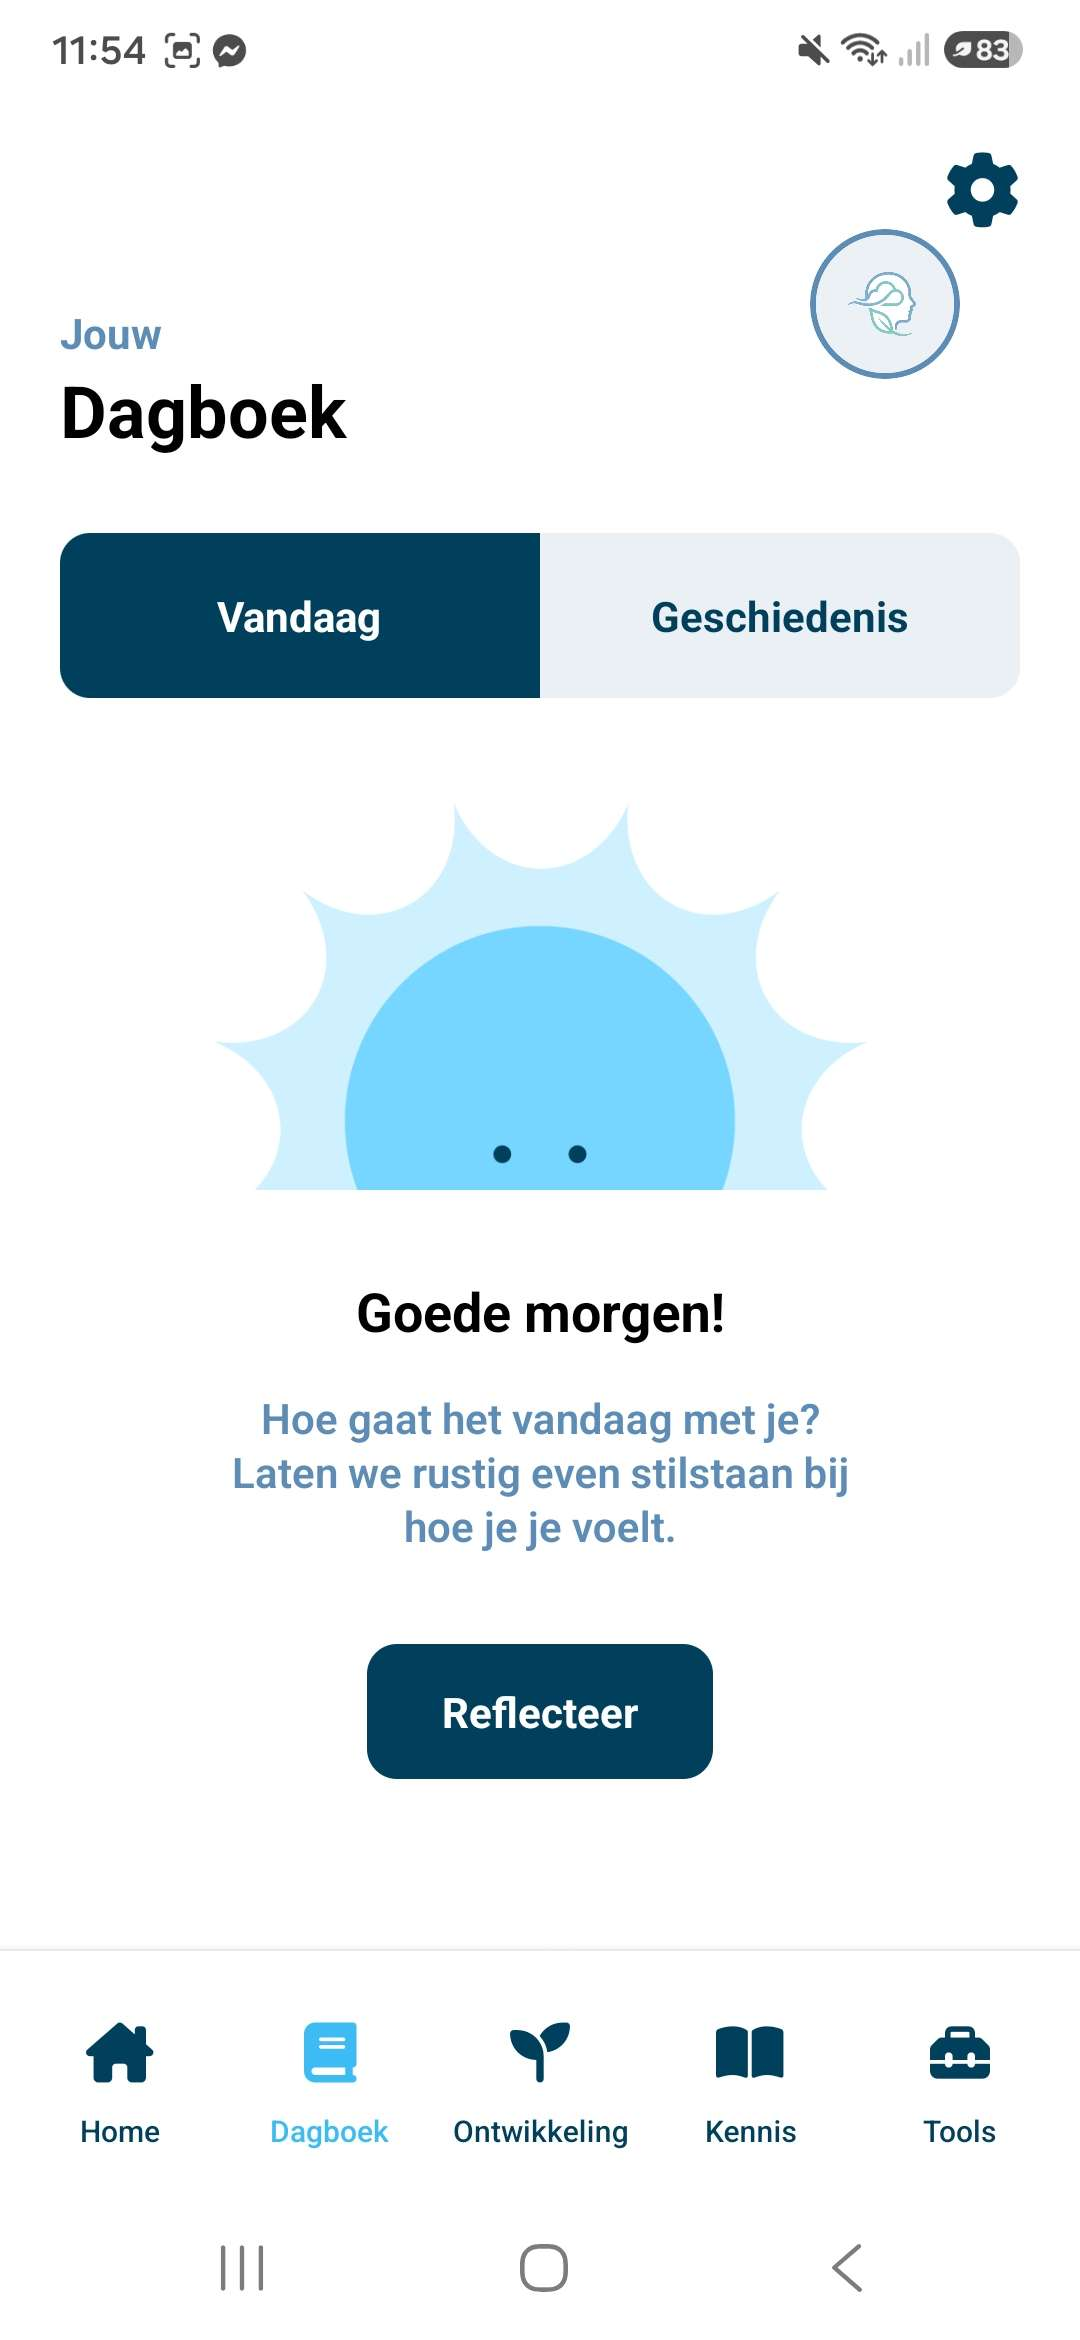
\includegraphics[width=\linewidth]{../graphics/Code/PoC8}
    \end{minipage}
    \hfill
    \begin{minipage}{0.3\textwidth}
        \centering
        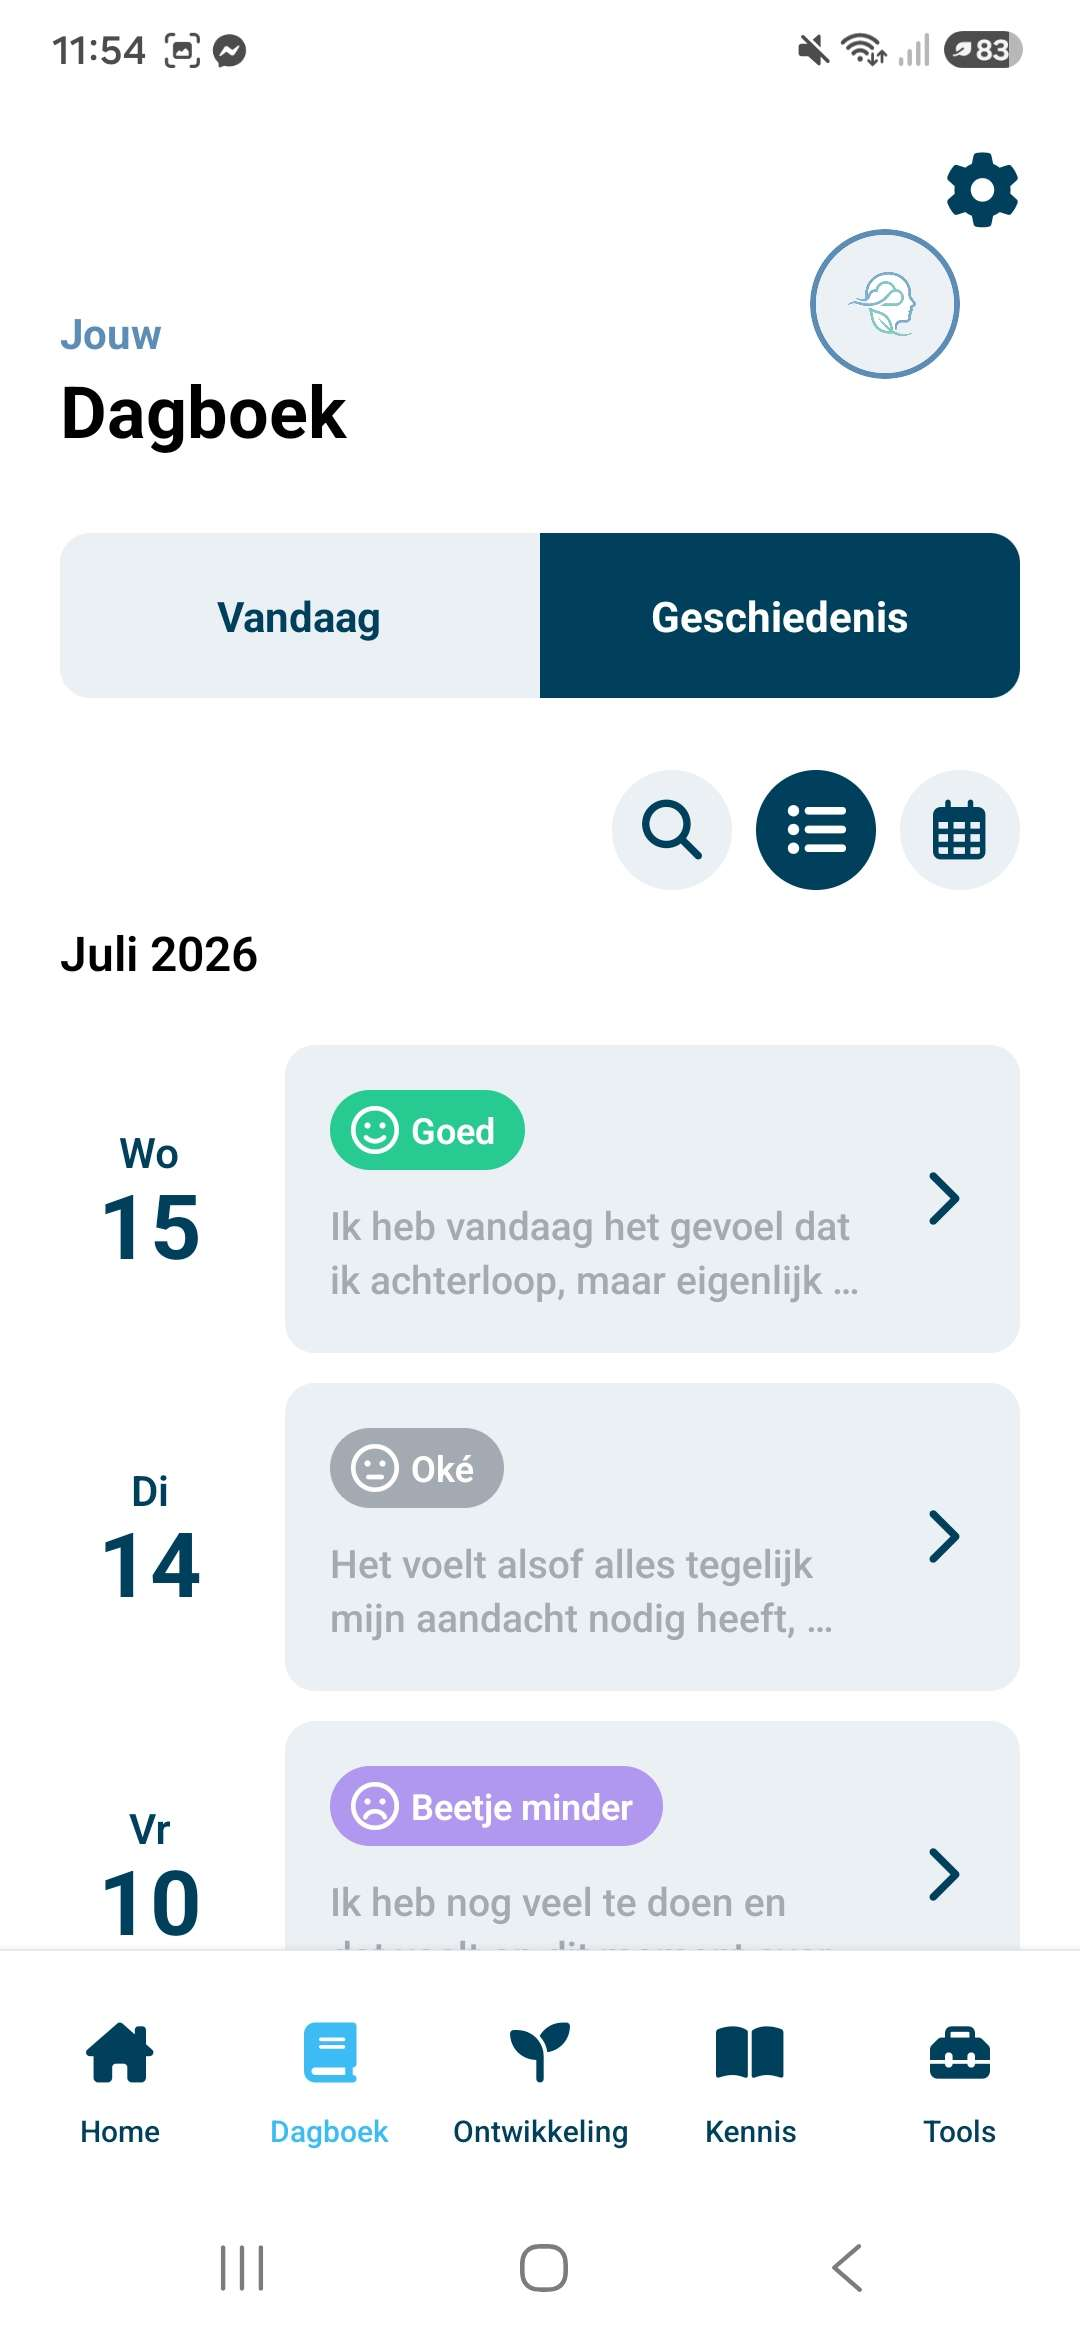
\includegraphics[width=\linewidth]{../graphics/Code/PoC9}
    \end{minipage}
    
    \vspace{1em}
    
    \begin{minipage}{0.3\textwidth}
        \centering
        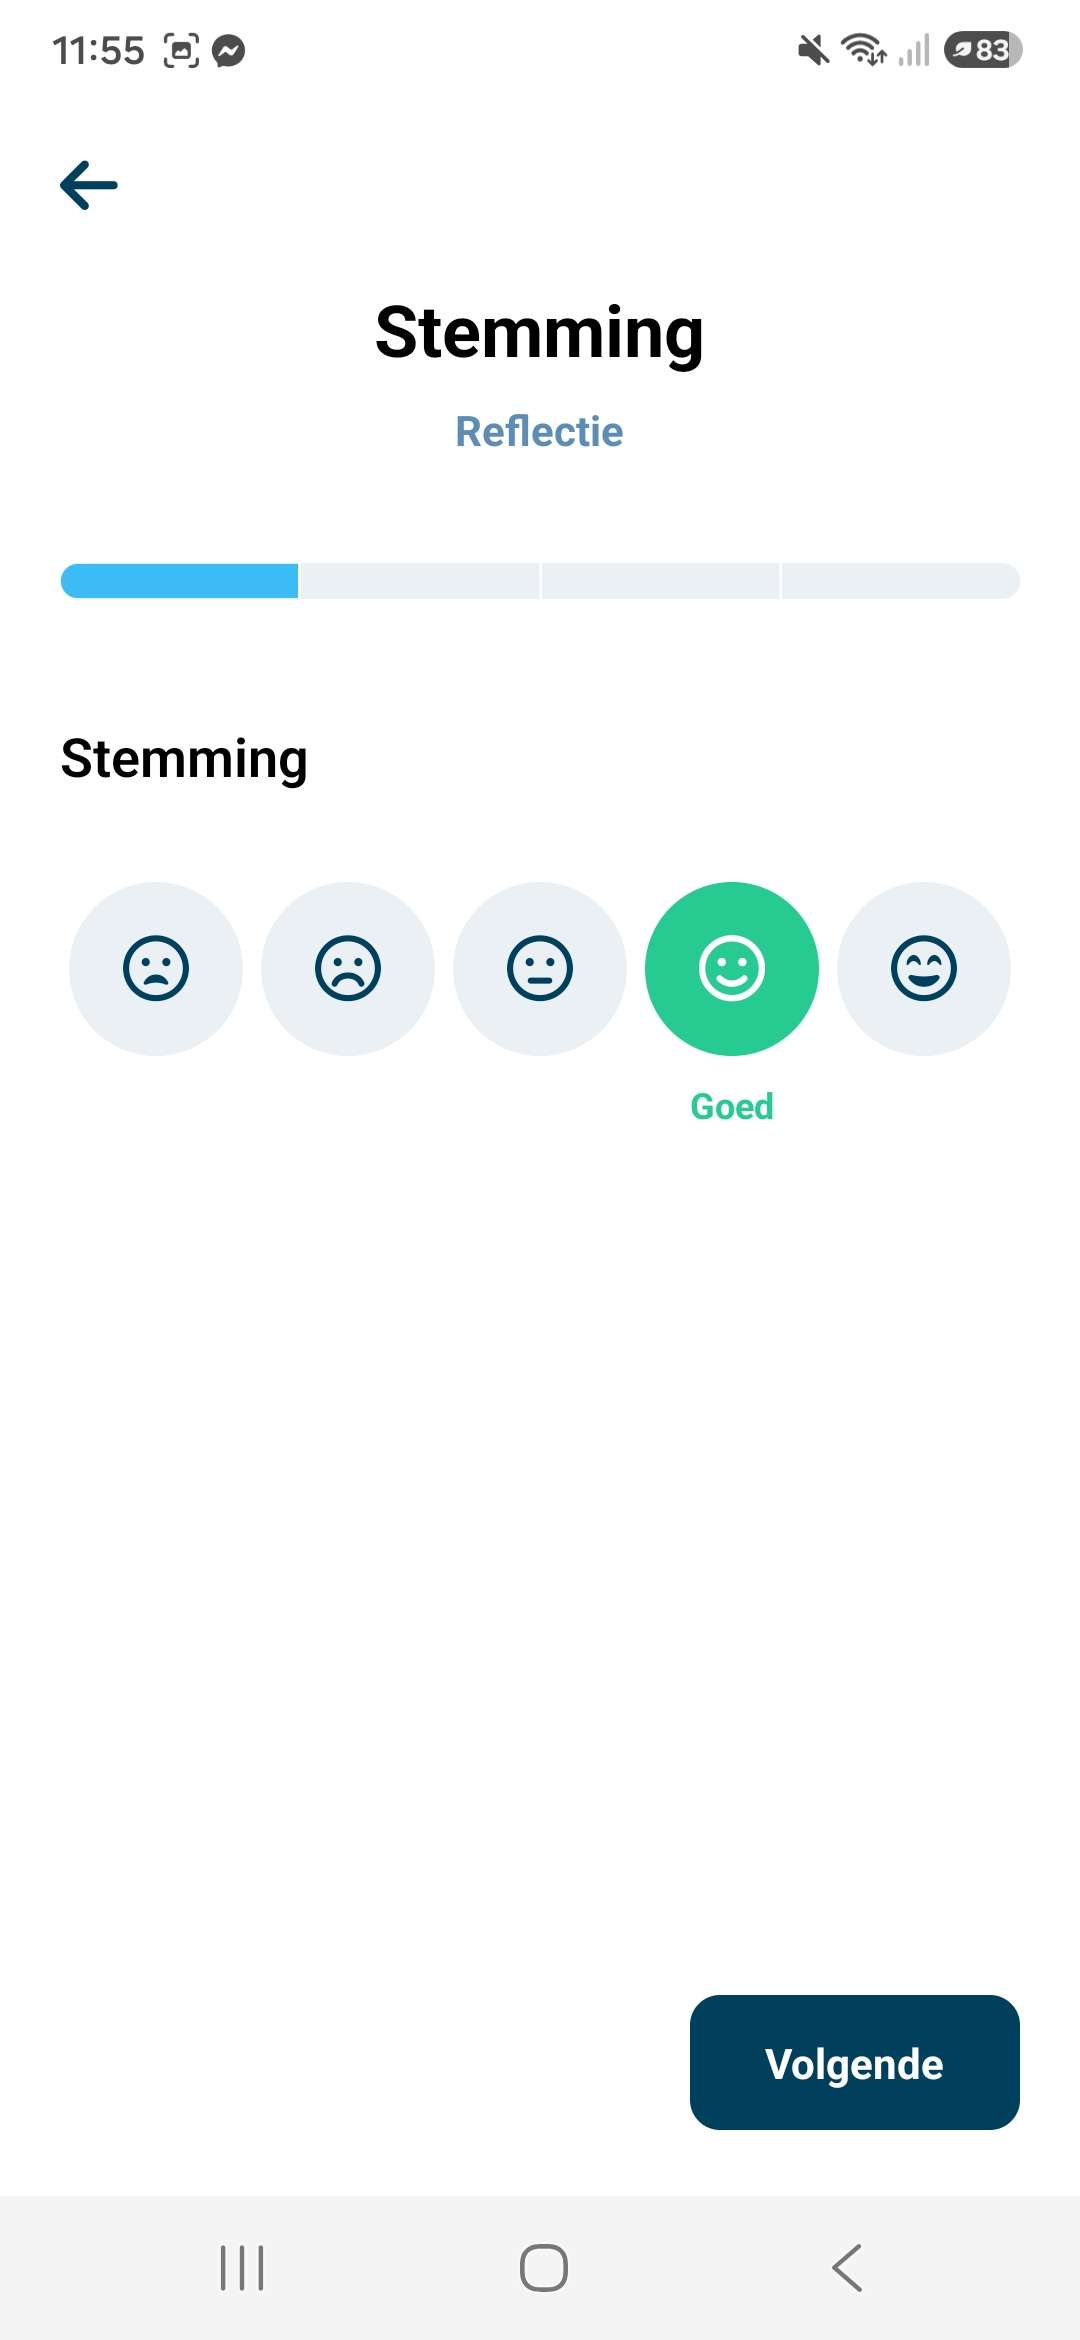
\includegraphics[width=\linewidth]{../graphics/Code/PoC10}
    \end{minipage}
    \hfill
    \begin{minipage}{0.3\textwidth}
        \centering
        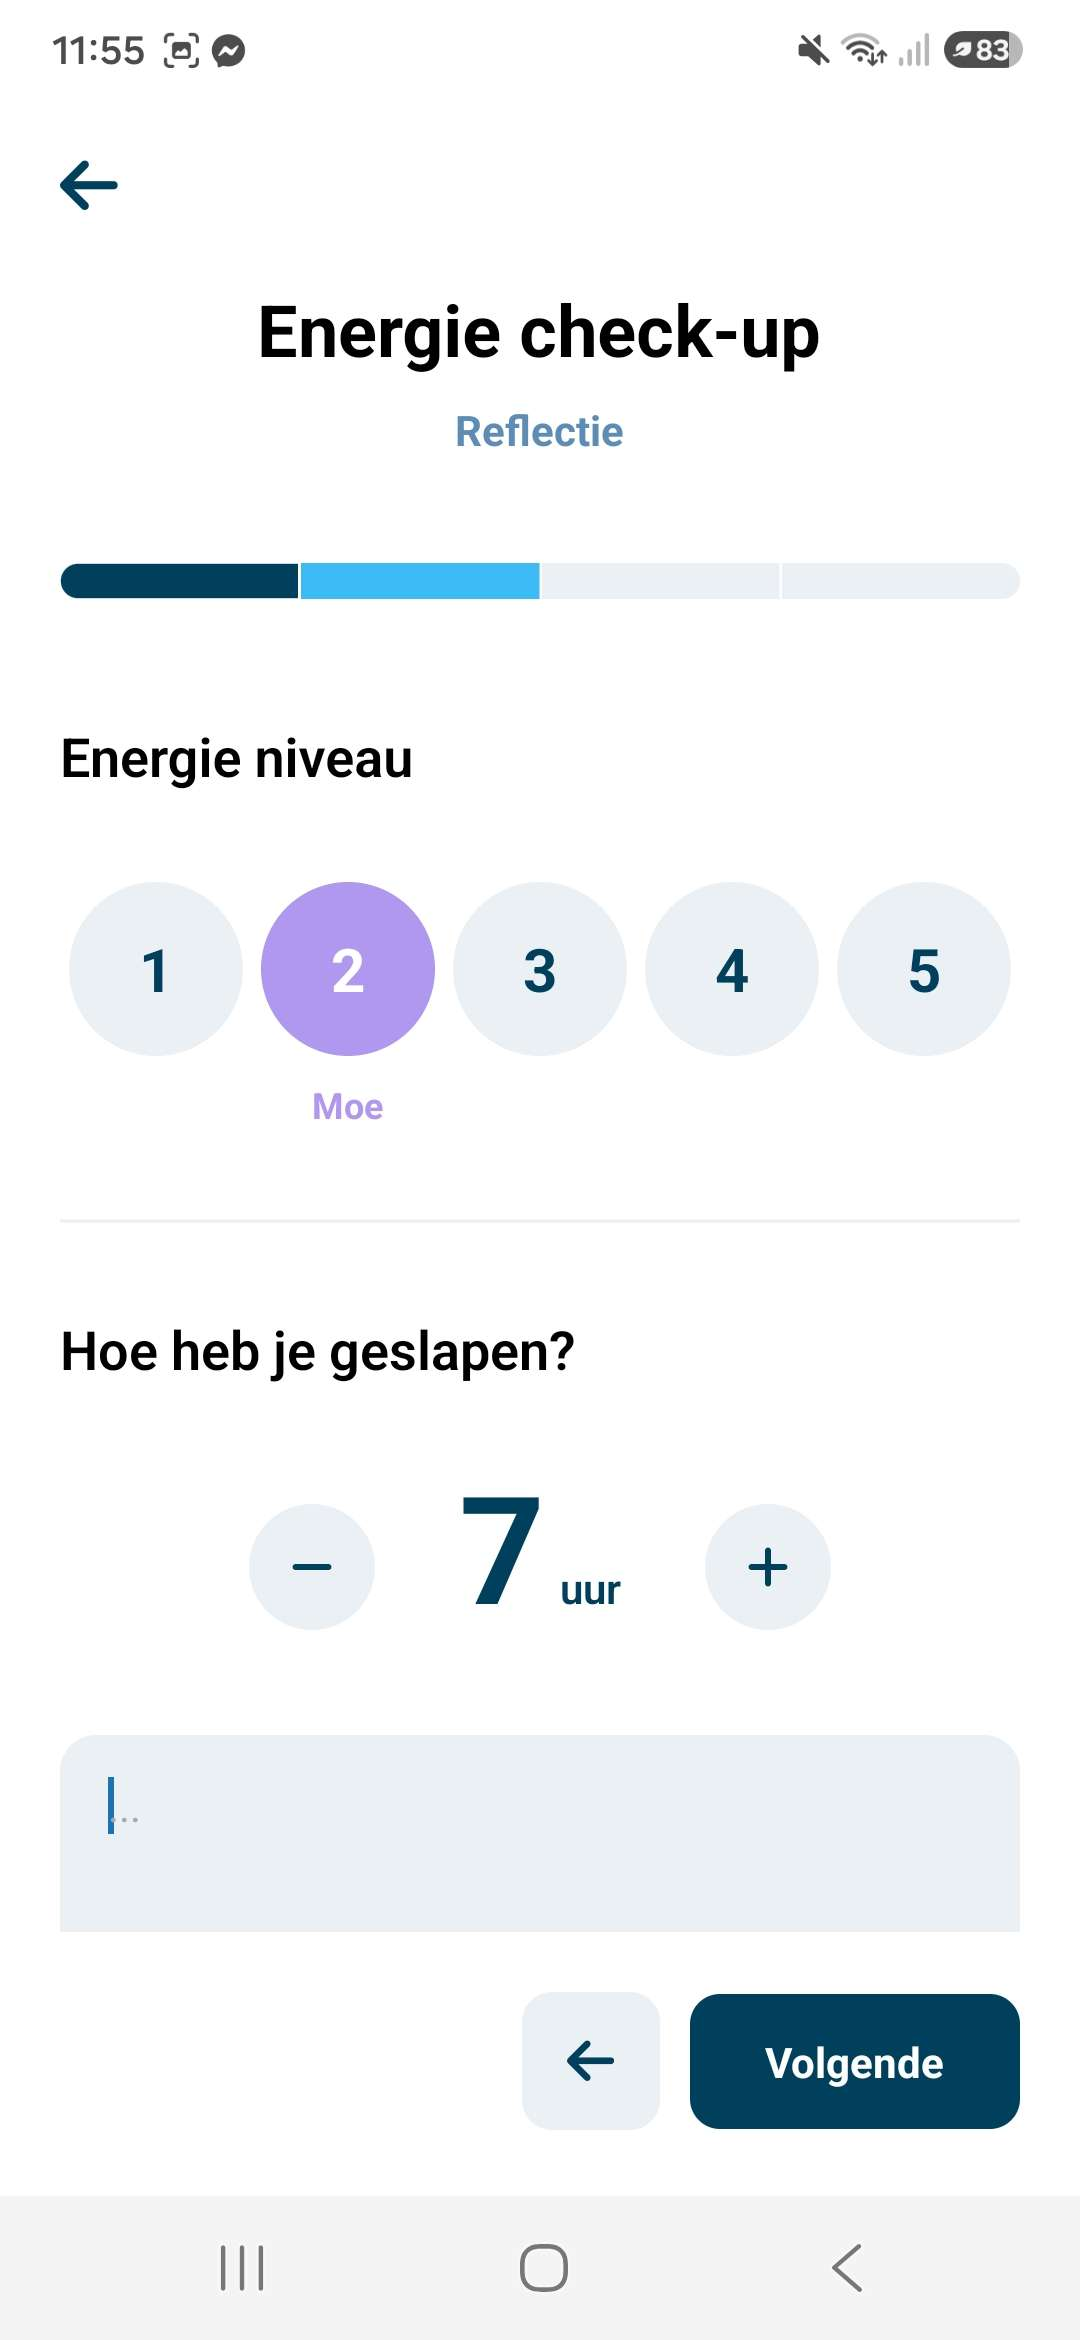
\includegraphics[width=\linewidth]{../graphics/Code/PoC11}
    \end{minipage}
    \hfill
    \begin{minipage}{0.3\textwidth}
        \centering
        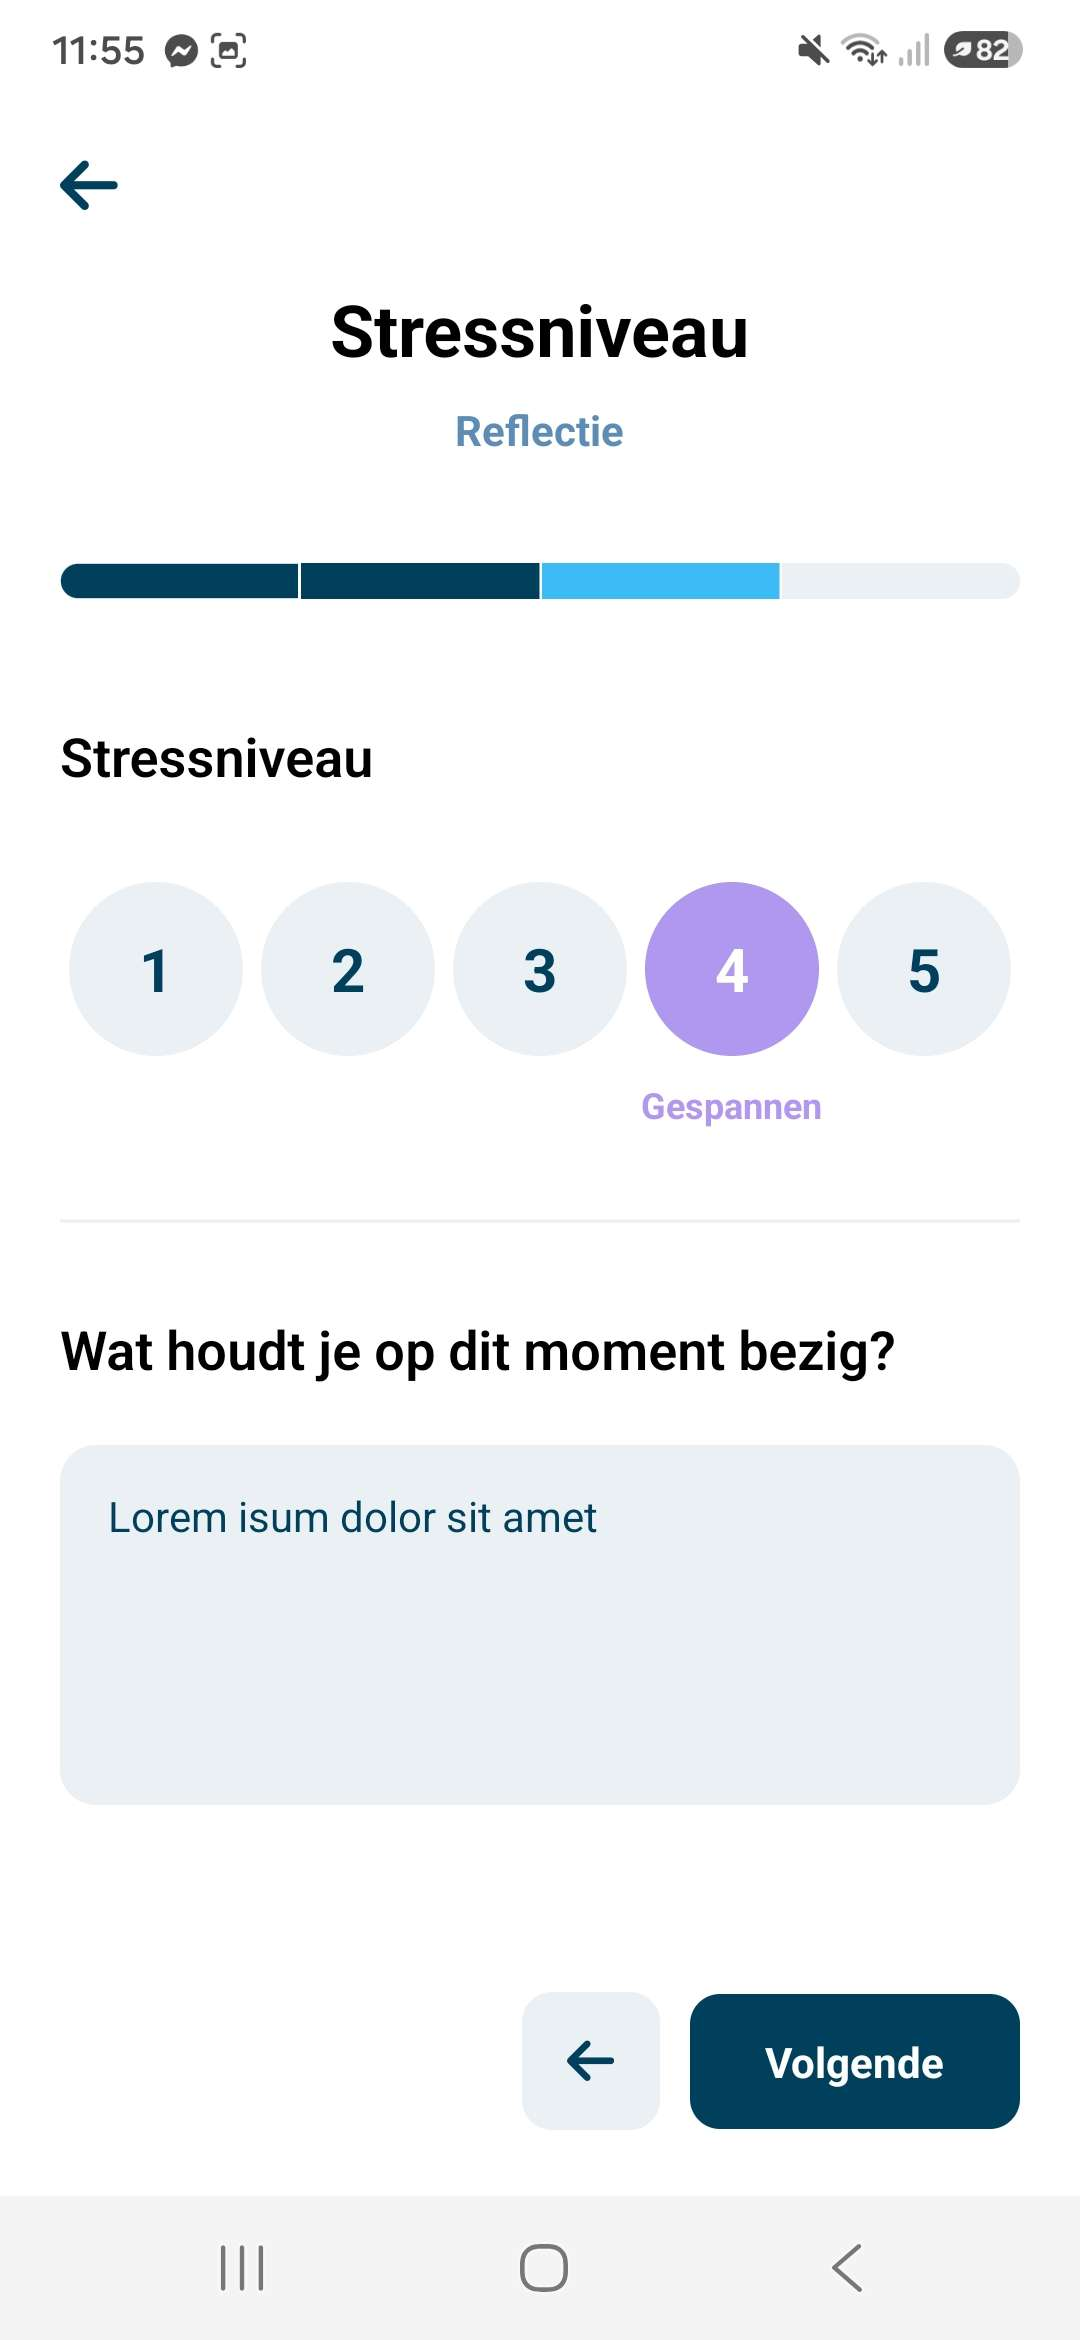
\includegraphics[width=\linewidth]{../graphics/Code/PoC12}
    \end{minipage}
    
    \caption{Overzicht van de tools, de dagboekpagina en de start van de reflectiefunctie binnen de applicatie.}
    \label{fig:code-ss-2}
\end{figure}

\begin{figure}[H]
    \centering
    
    \begin{minipage}{0.3\textwidth}
        \centering
        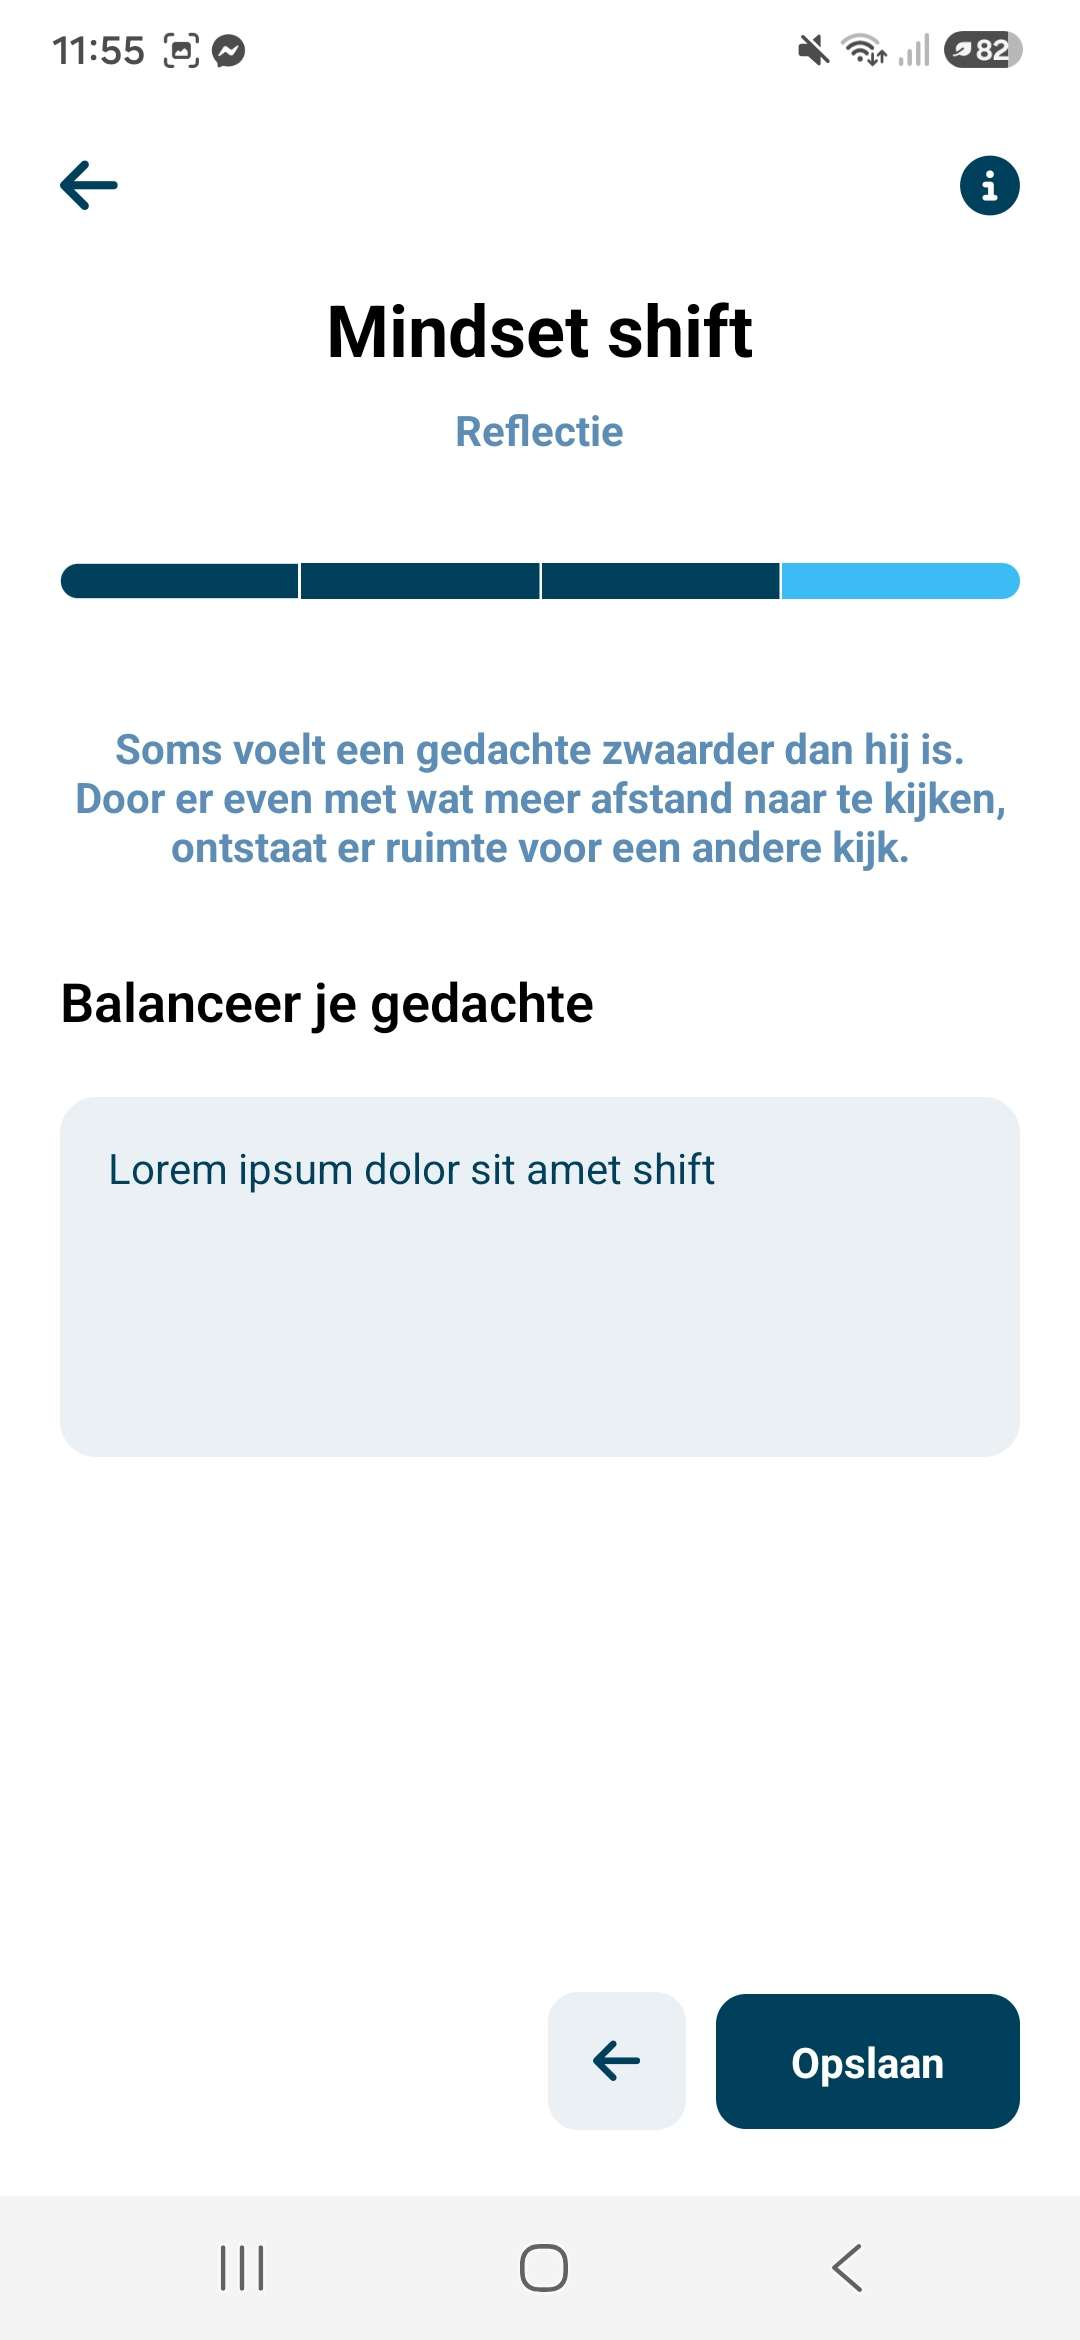
\includegraphics[width=\linewidth]{../graphics/Code/PoC13}
    \end{minipage}
    \hfill
    \begin{minipage}{0.3\textwidth}
        \centering
        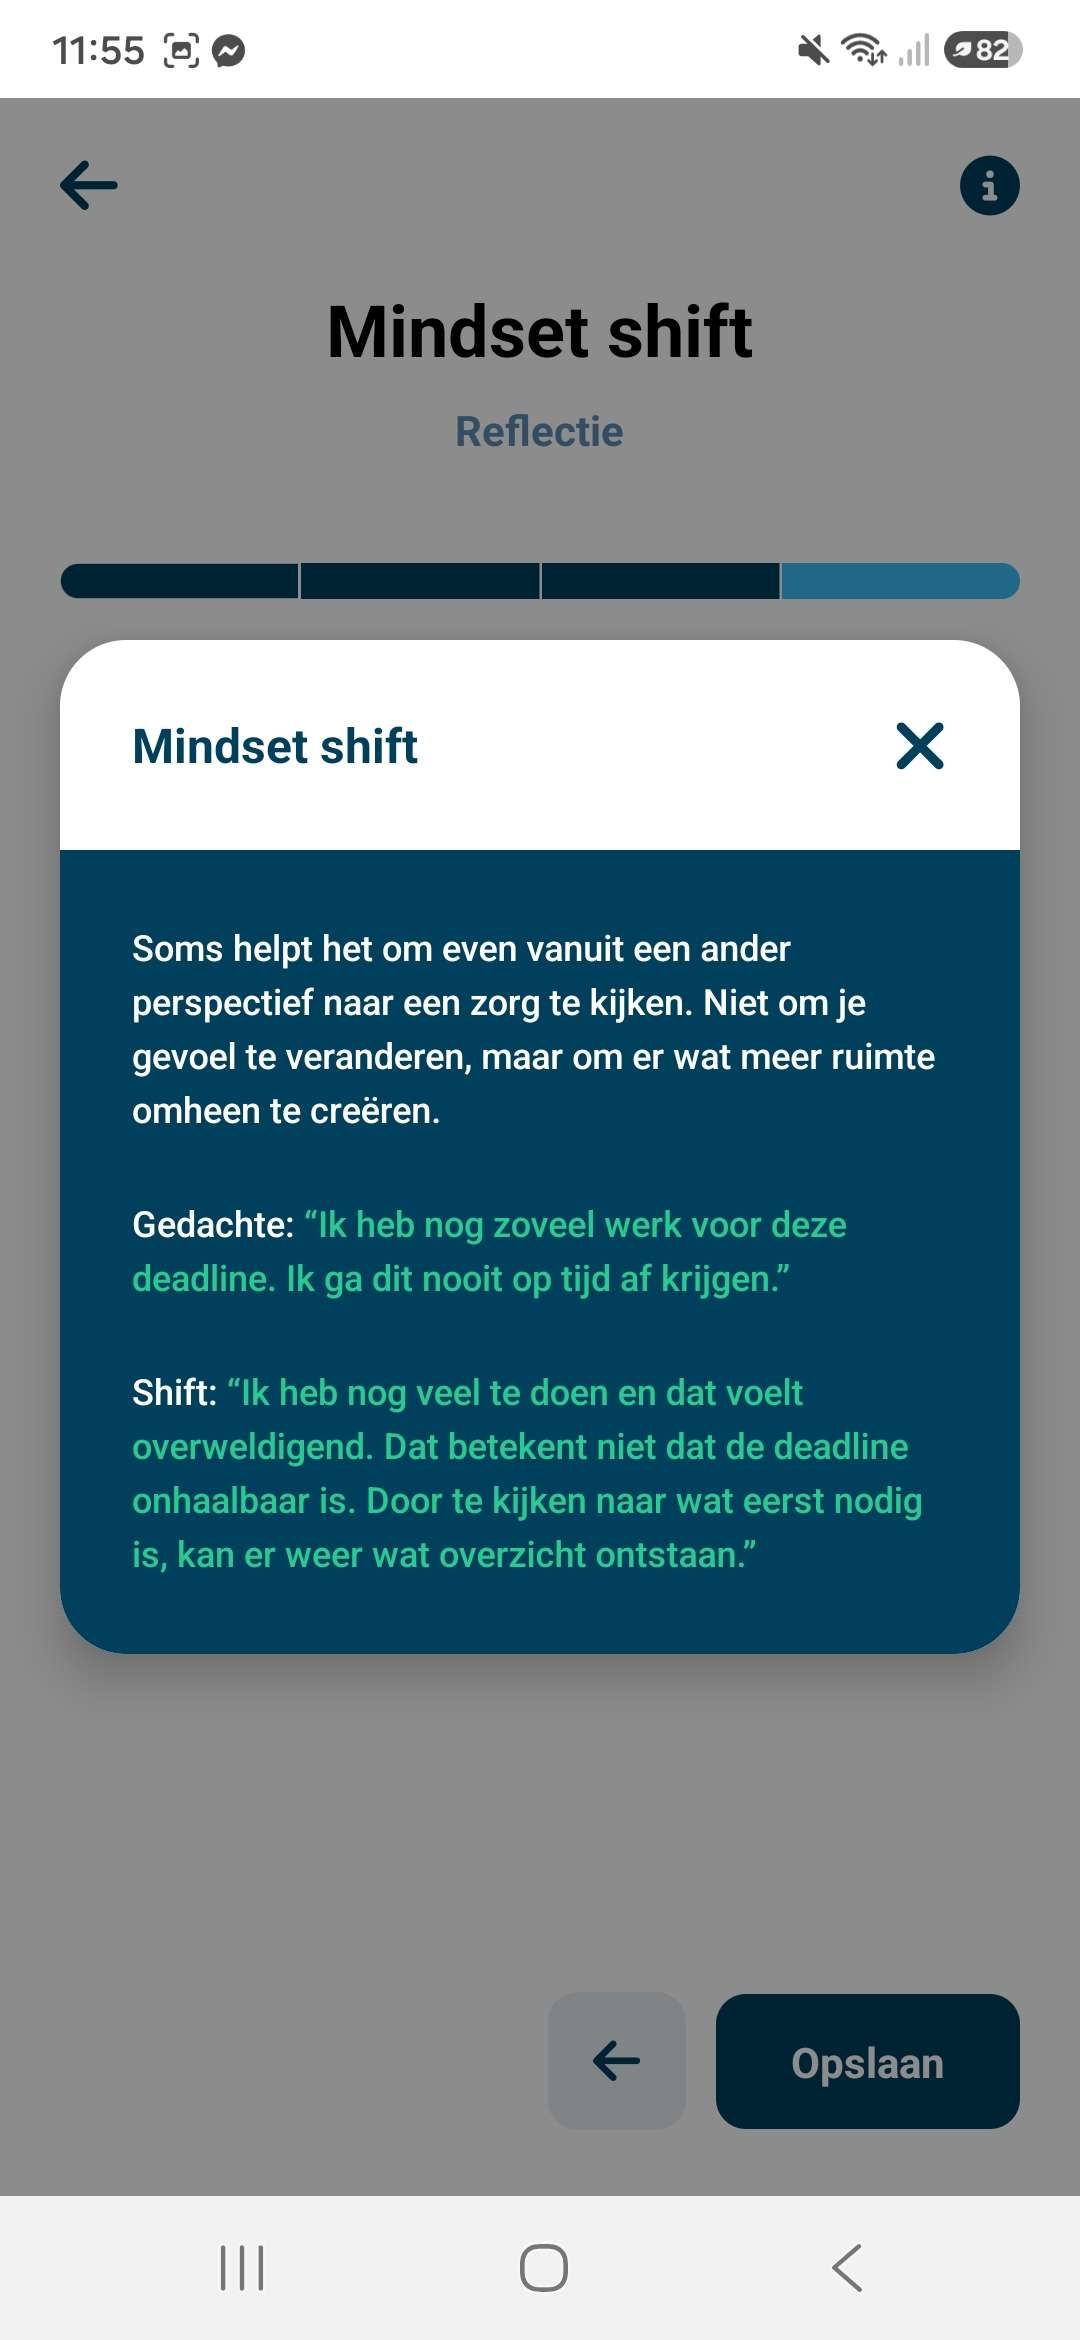
\includegraphics[width=\linewidth]{../graphics/Code/PoC14}
    \end{minipage}
    \hfill
    \begin{minipage}{0.3\textwidth}
        \centering
        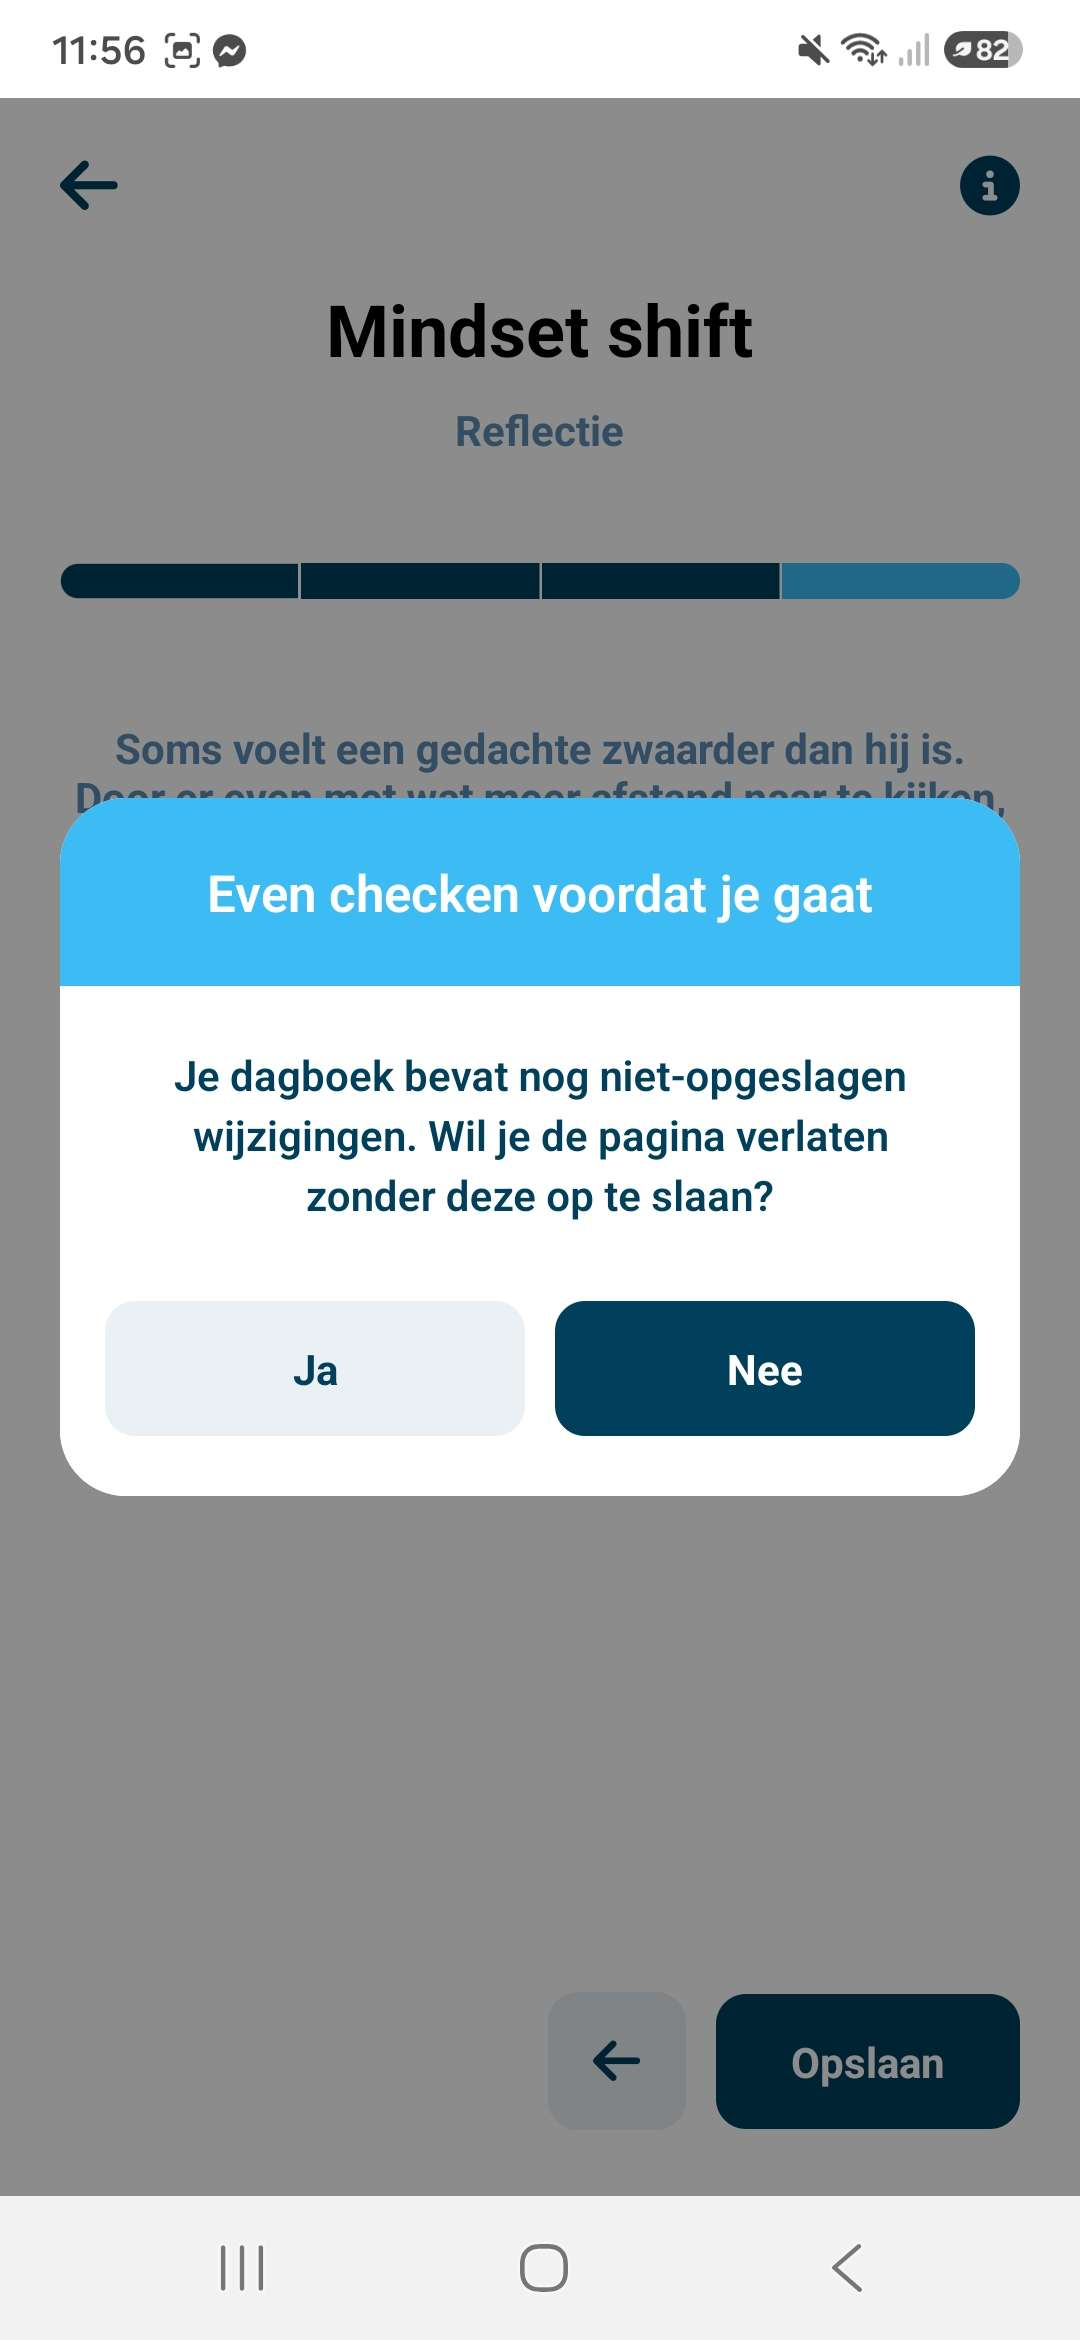
\includegraphics[width=\linewidth]{../graphics/Code/PoC15}
    \end{minipage}
    
    \vspace{1em}
    
    \begin{minipage}{0.3\textwidth}
        \centering
        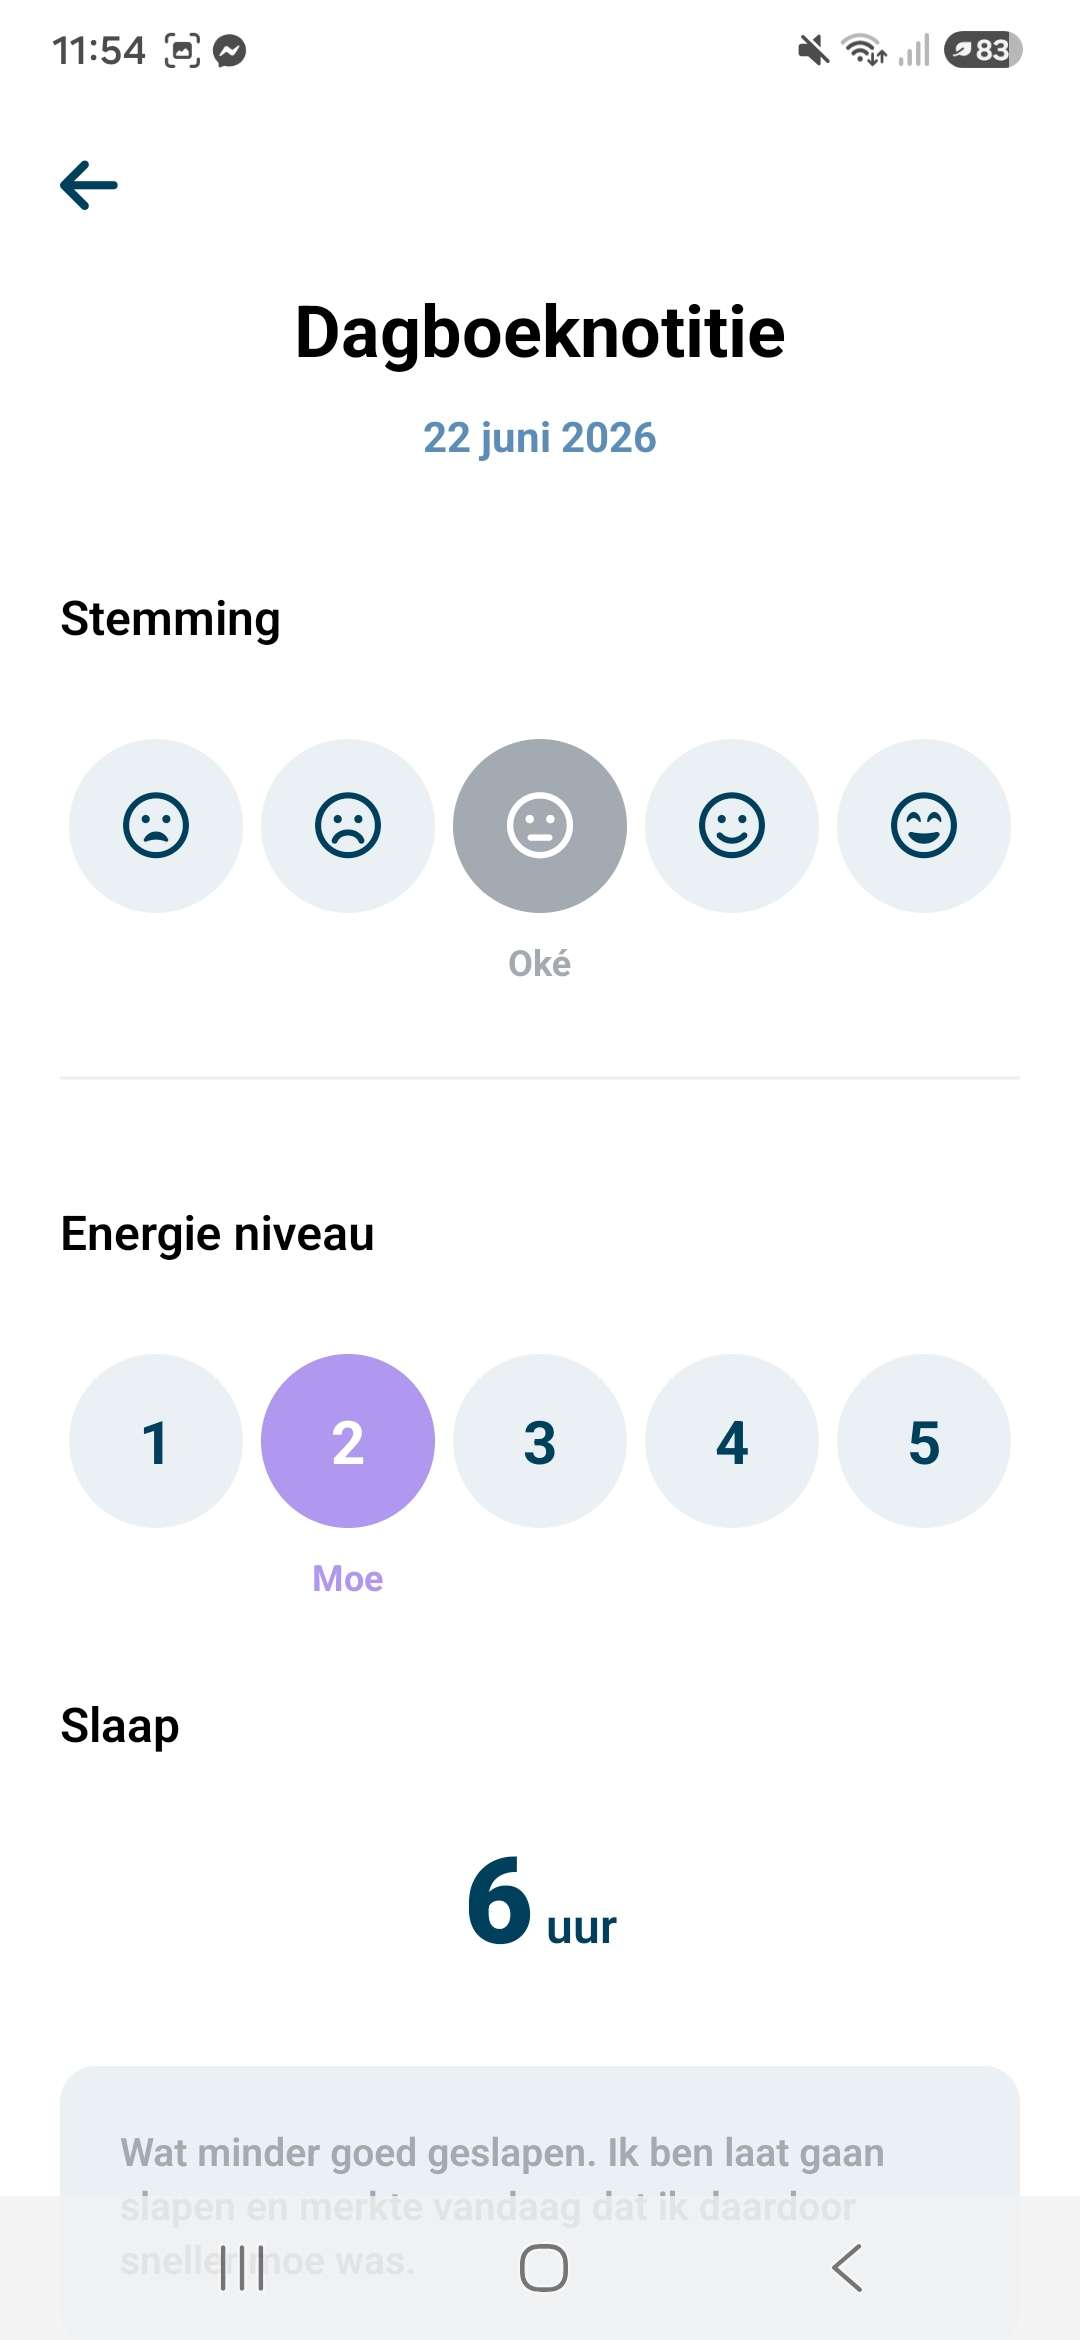
\includegraphics[width=\linewidth]{../graphics/Code/PoC16}
    \end{minipage}
    \hfill
    \begin{minipage}{0.3\textwidth}
        \centering
        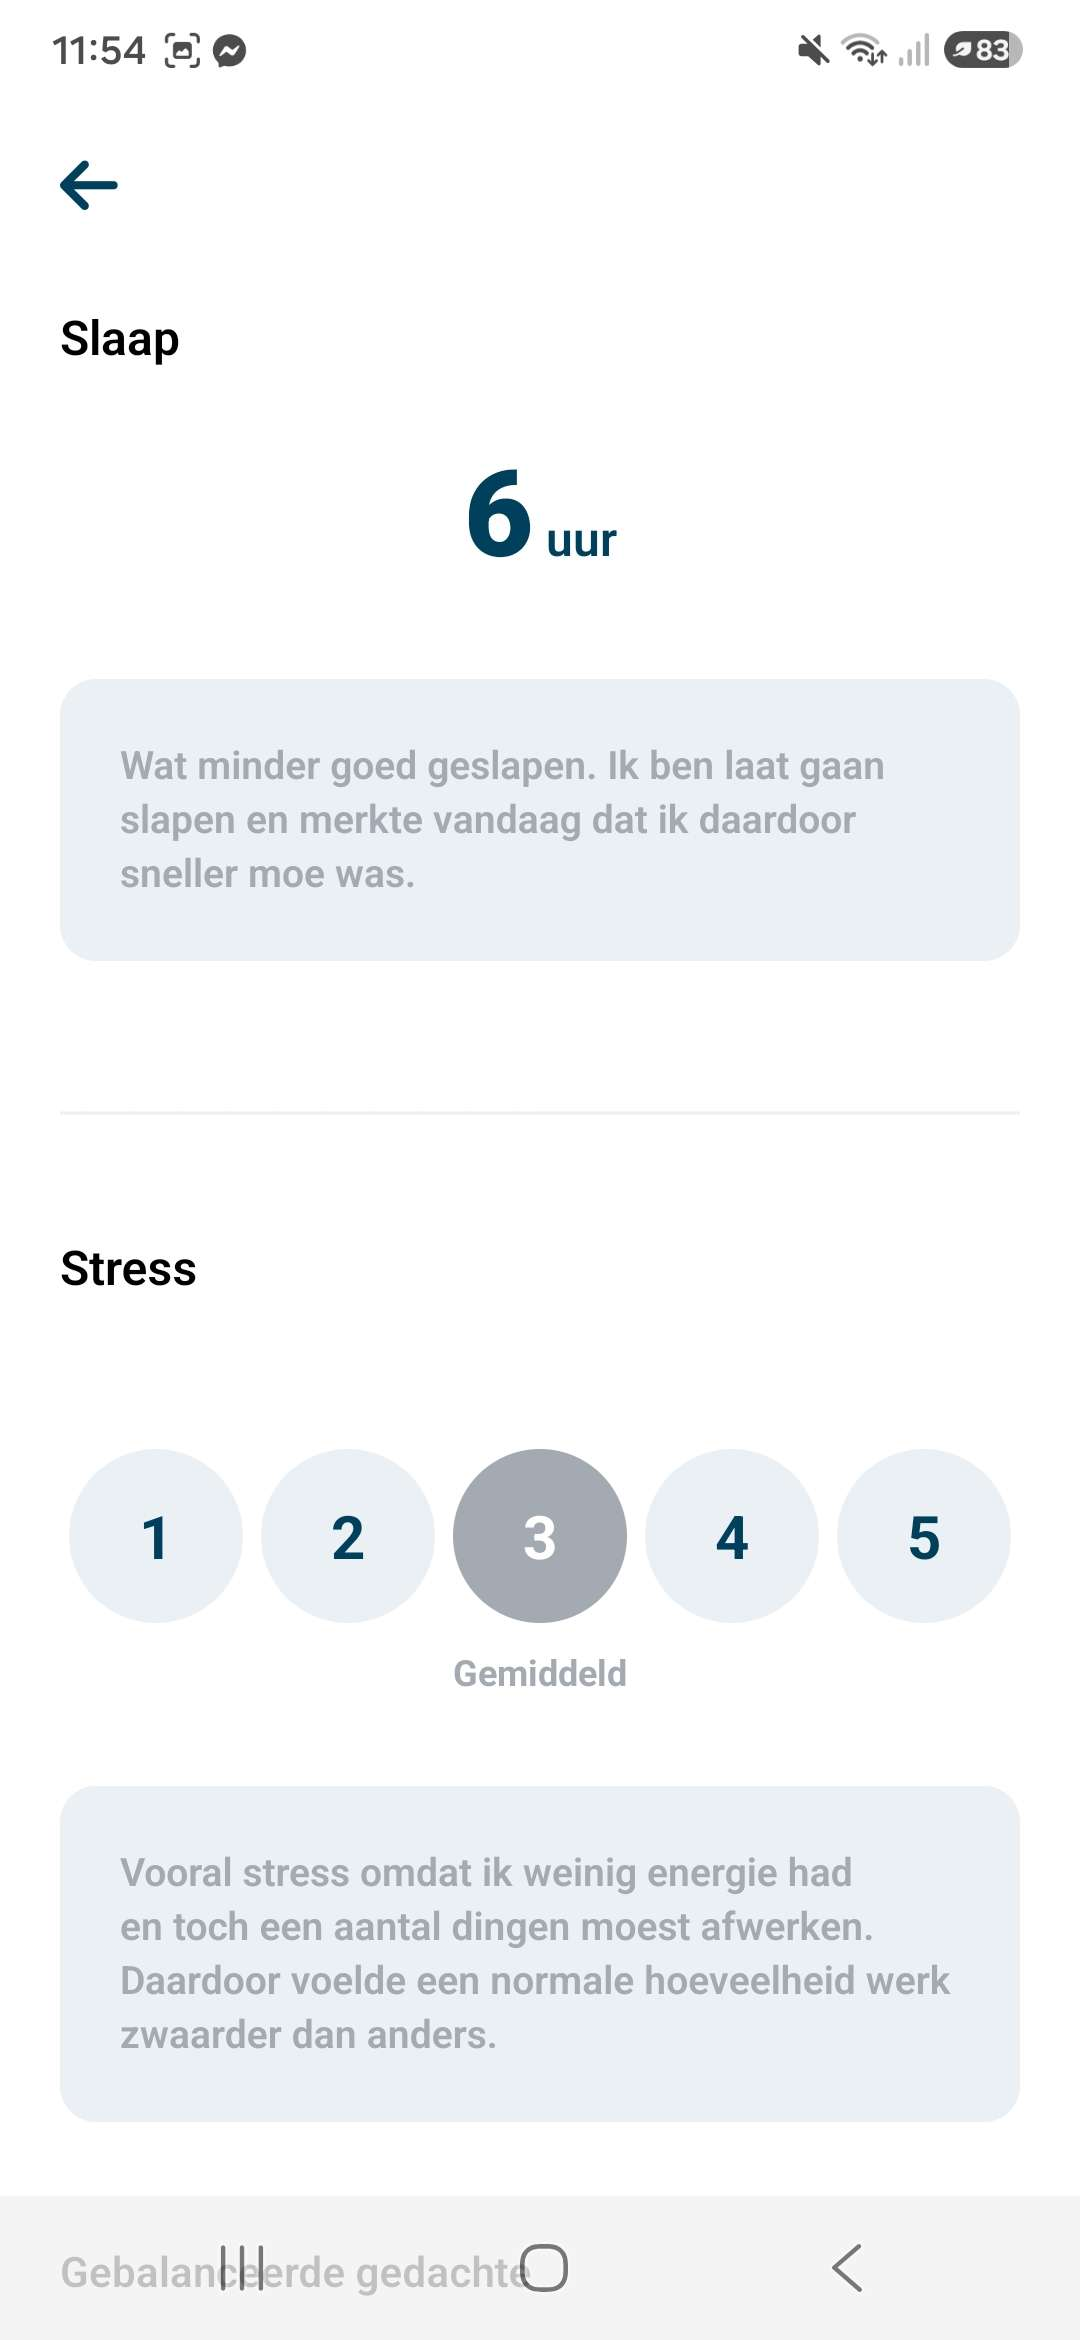
\includegraphics[width=\linewidth]{../graphics/Code/PoC17}
    \end{minipage}
    \hfill
    \begin{minipage}{0.3\textwidth}
        \centering
        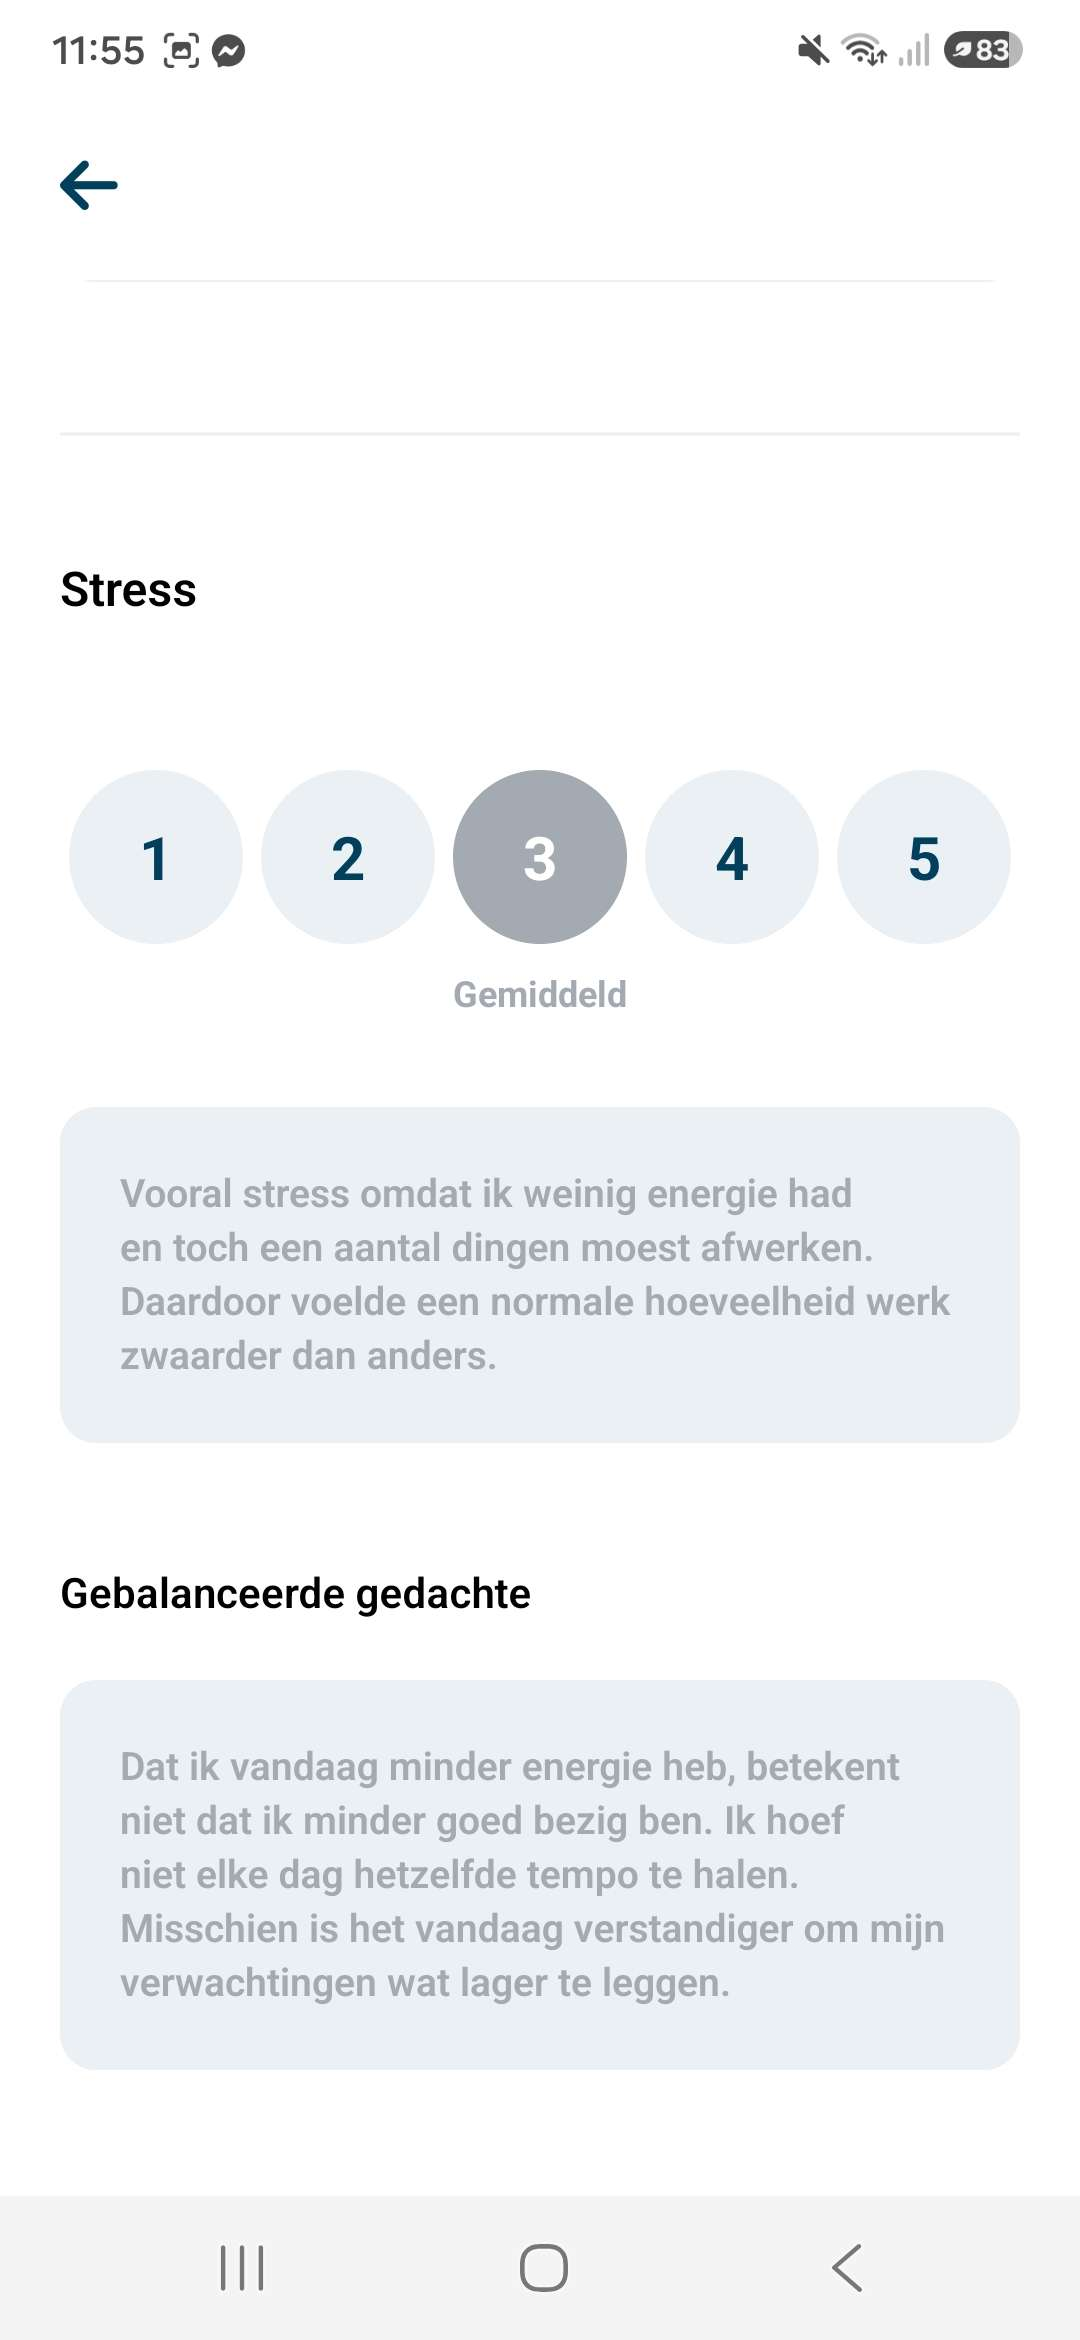
\includegraphics[width=\linewidth]{../graphics/Code/PoC18}
    \end{minipage}
    
    \caption{Vervolg van de reflectiefunctie en de detailweergave van een individuele dagboeknotitie.}
    \label{fig:code-ss-3}
\end{figure}

\begin{figure}[H]
    \centering
    
    \begin{minipage}{0.3\textwidth}
        \centering
        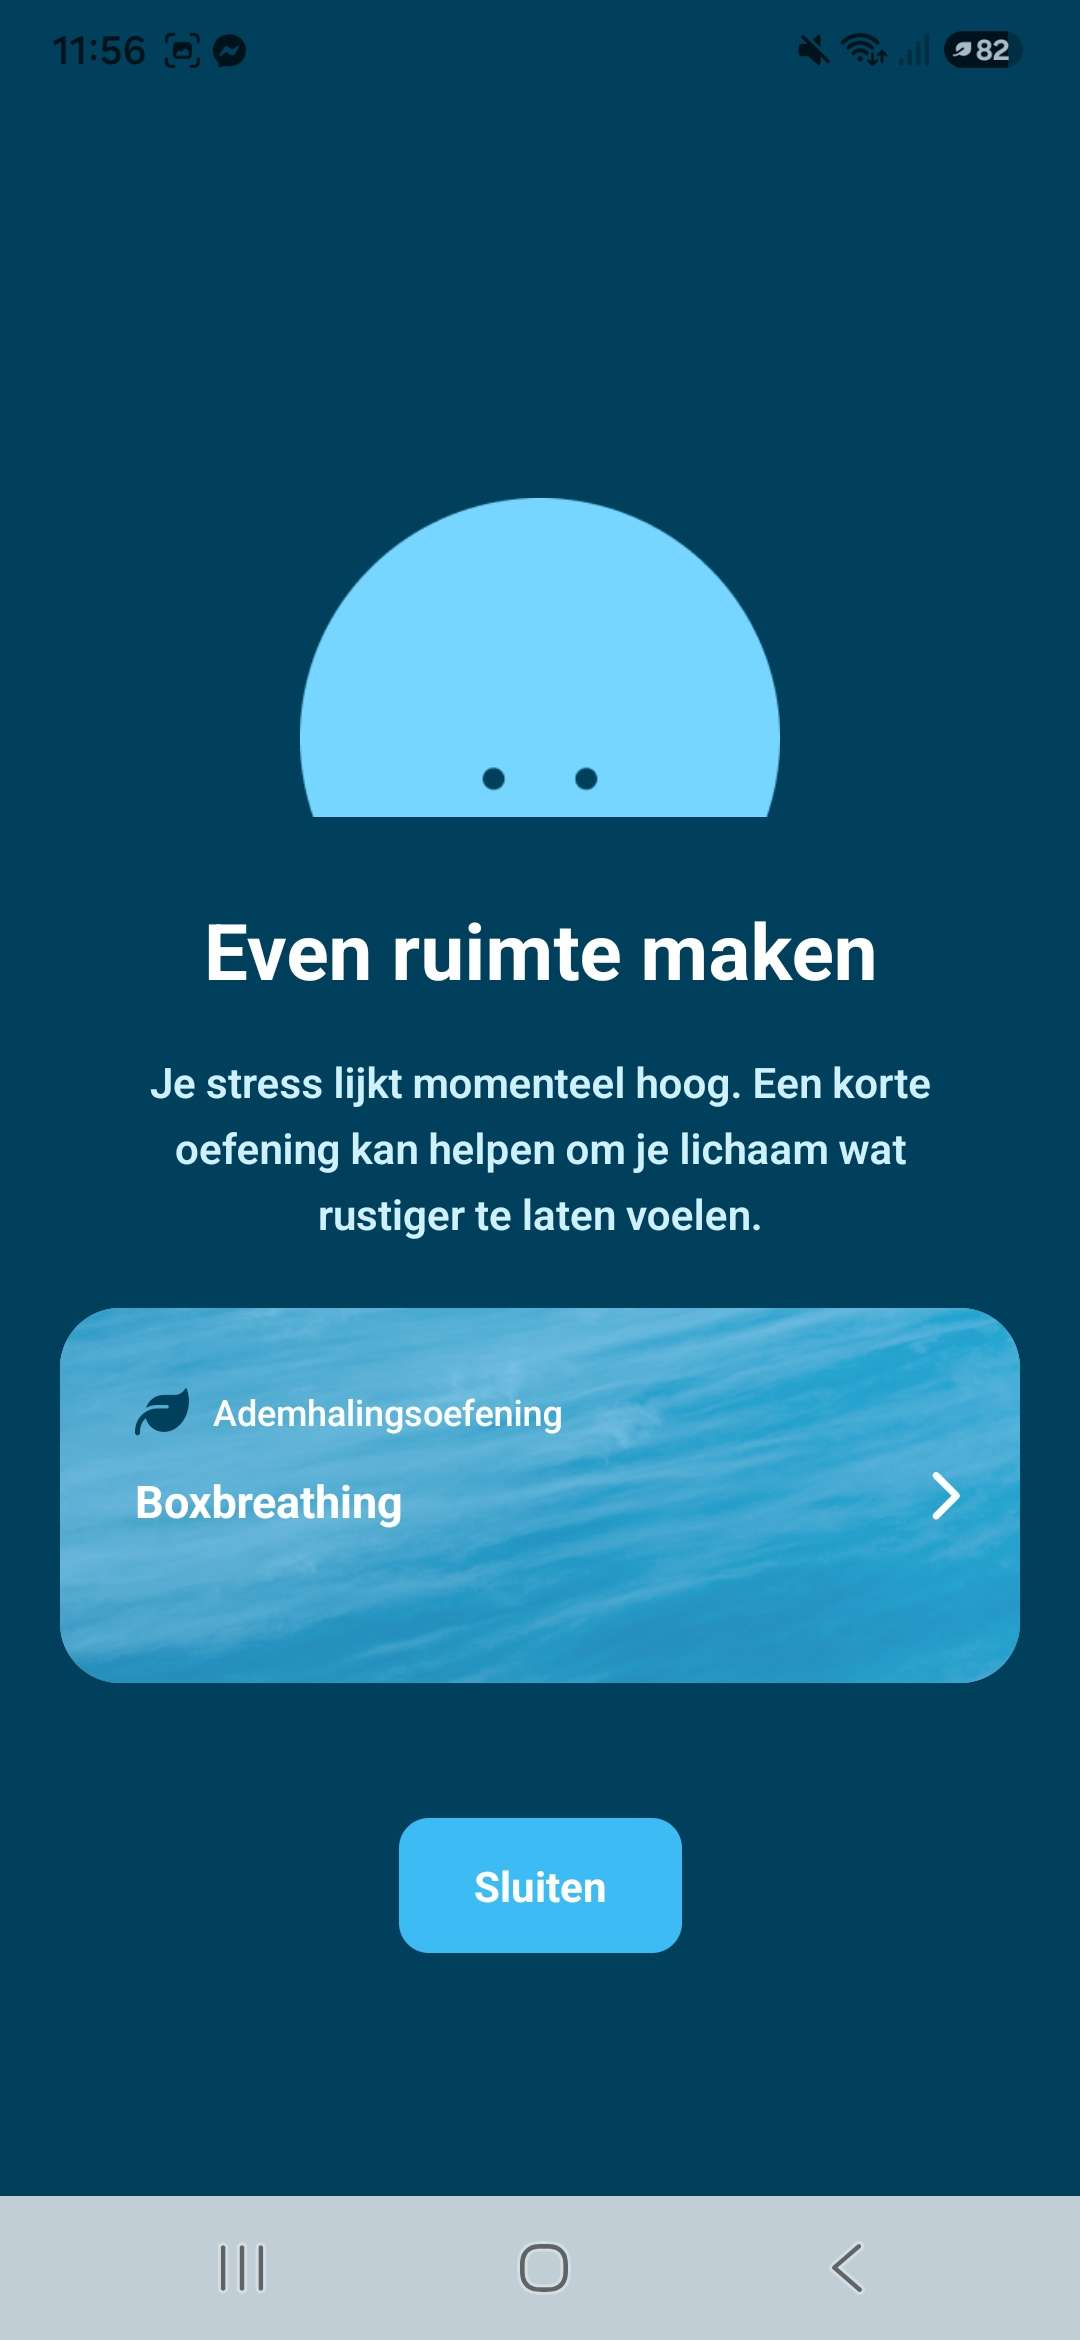
\includegraphics[width=\linewidth]{../graphics/Code/PoC19}
    \end{minipage}
    \hfill
    \begin{minipage}{0.3\textwidth}
        \centering
        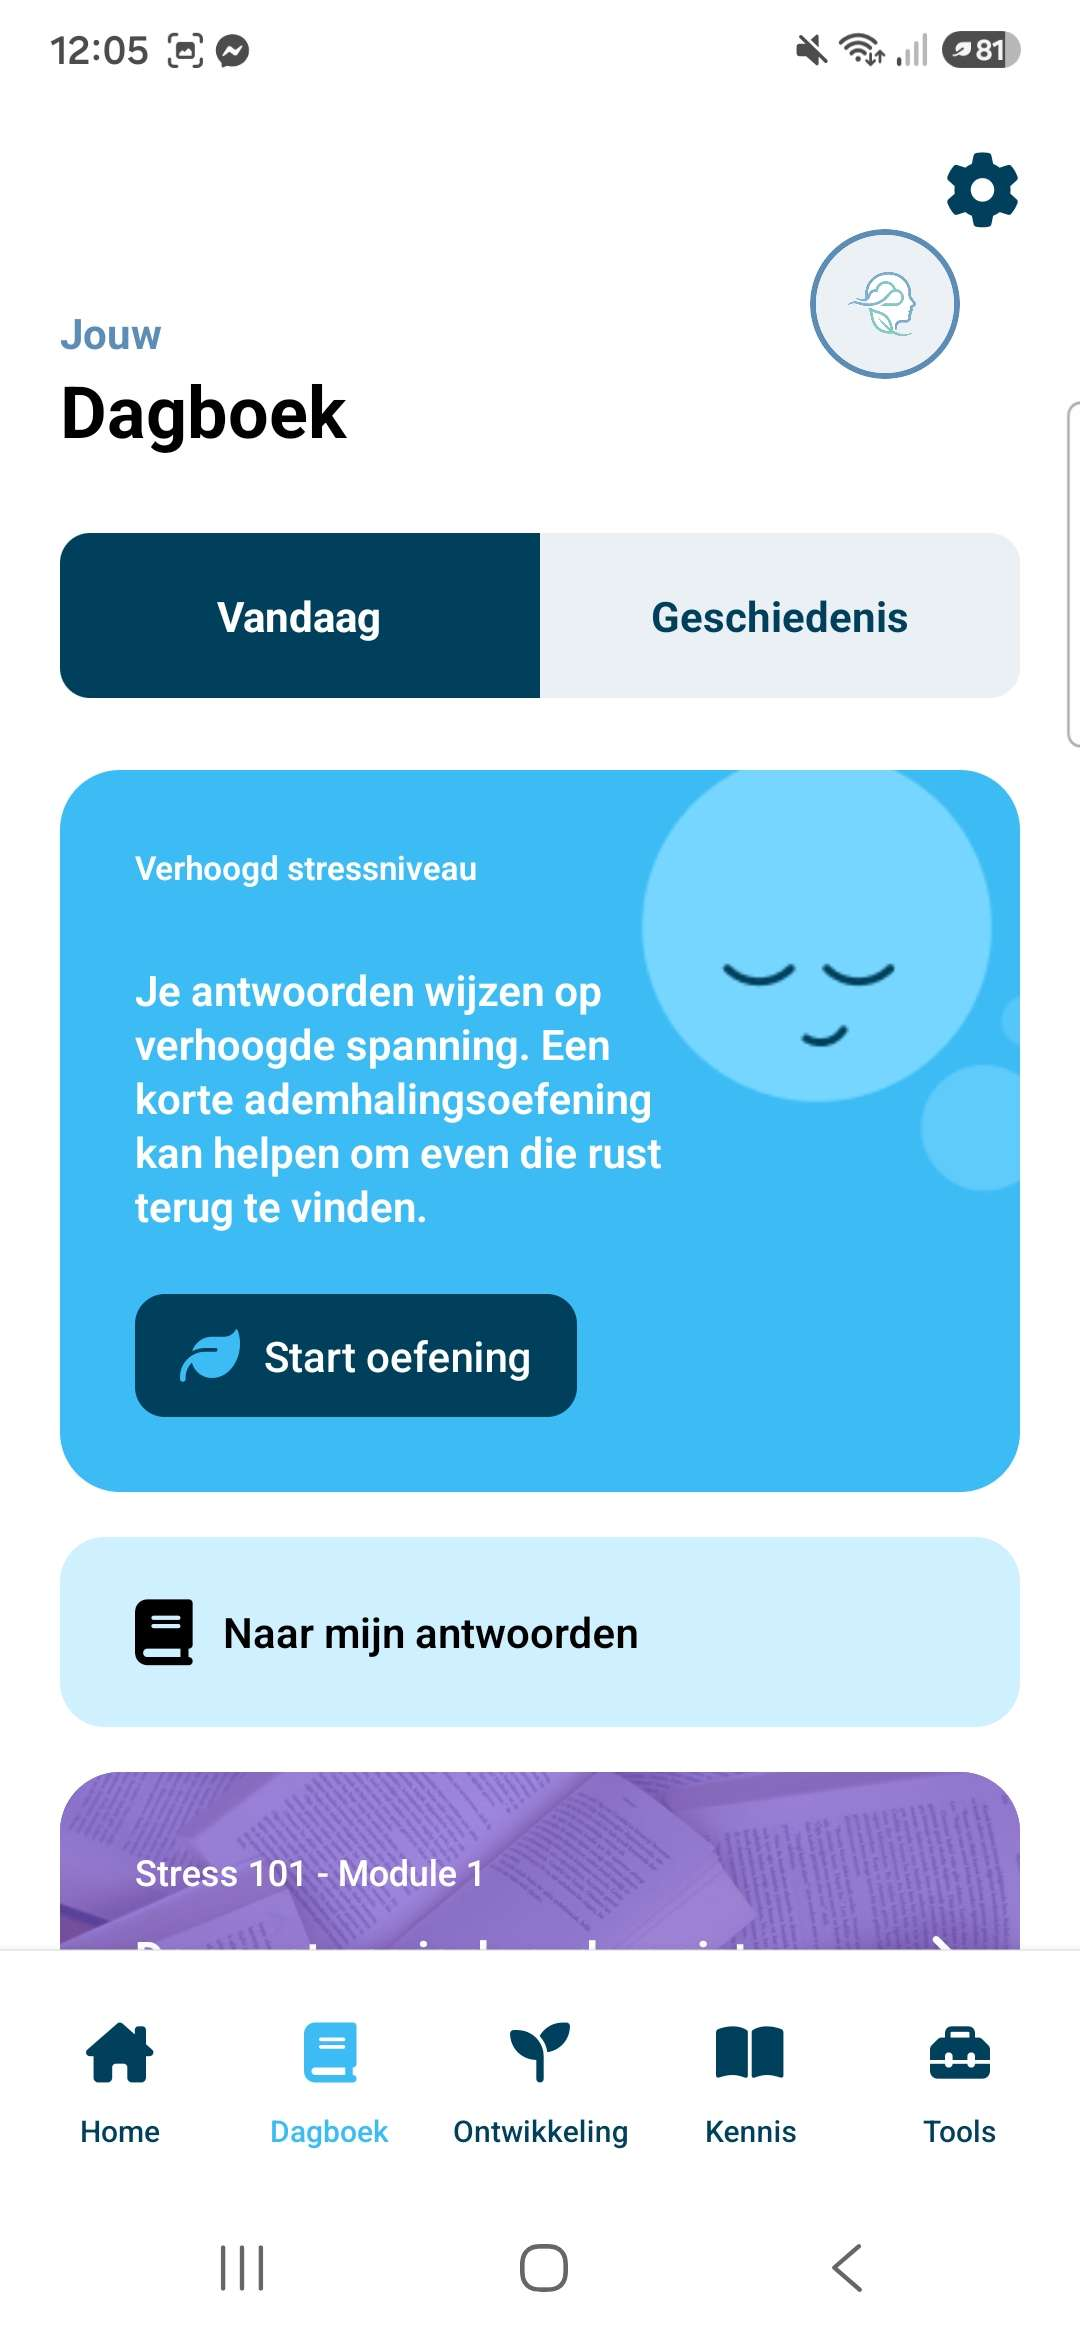
\includegraphics[width=\linewidth]{../graphics/Code/PoC20}
    \end{minipage}
    \hfill
    \begin{minipage}{0.3\textwidth}
        \centering
        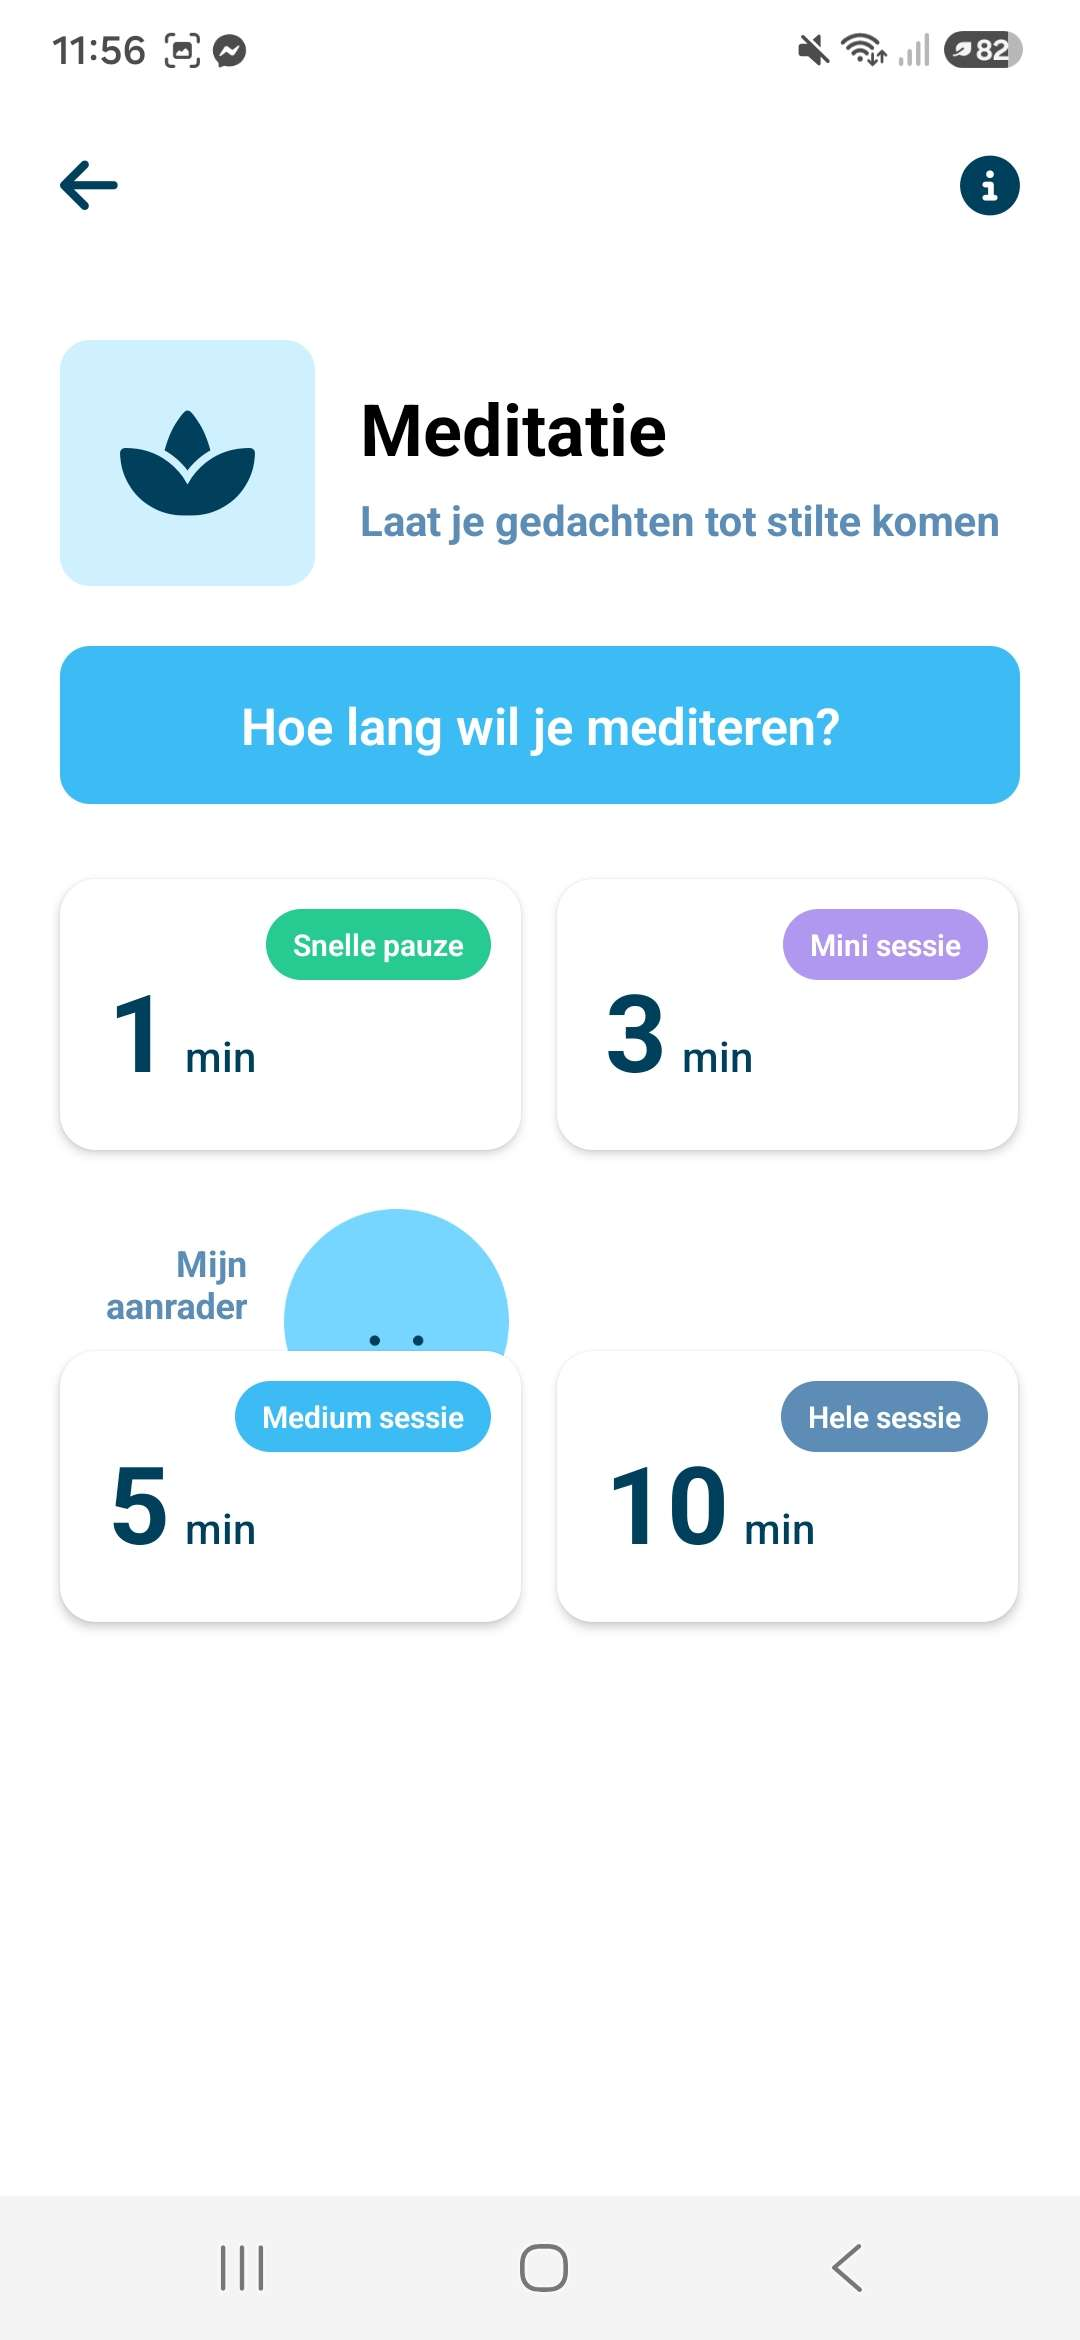
\includegraphics[width=\linewidth]{../graphics/Code/PoC21}
    \end{minipage}
    
    \vspace{1em}
    
    \begin{minipage}{0.3\textwidth}
        \centering
        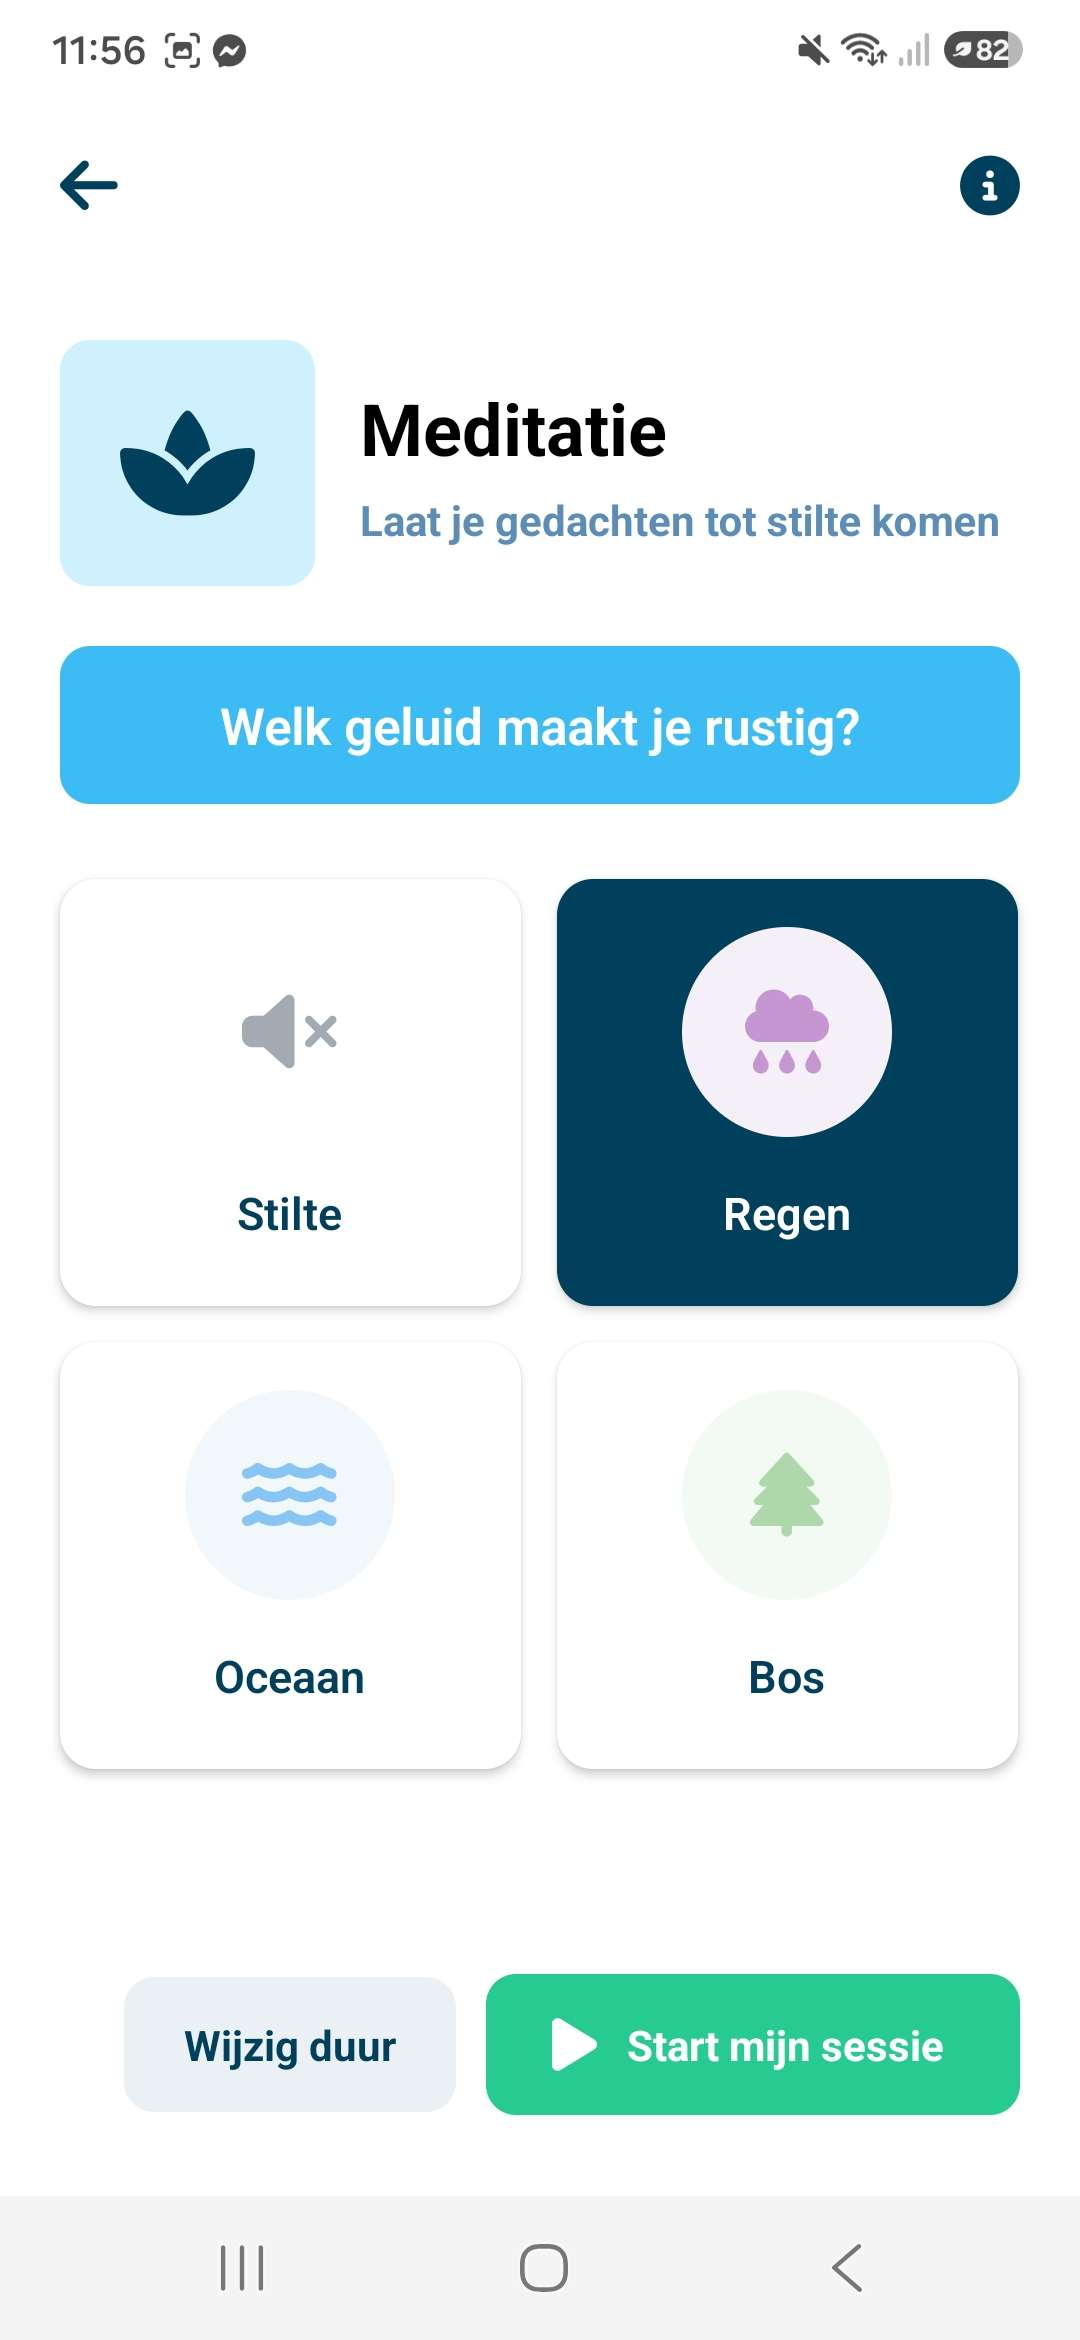
\includegraphics[width=\linewidth]{../graphics/Code/PoC22}
    \end{minipage}
    \hfill
    \begin{minipage}{0.3\textwidth}
        \centering
        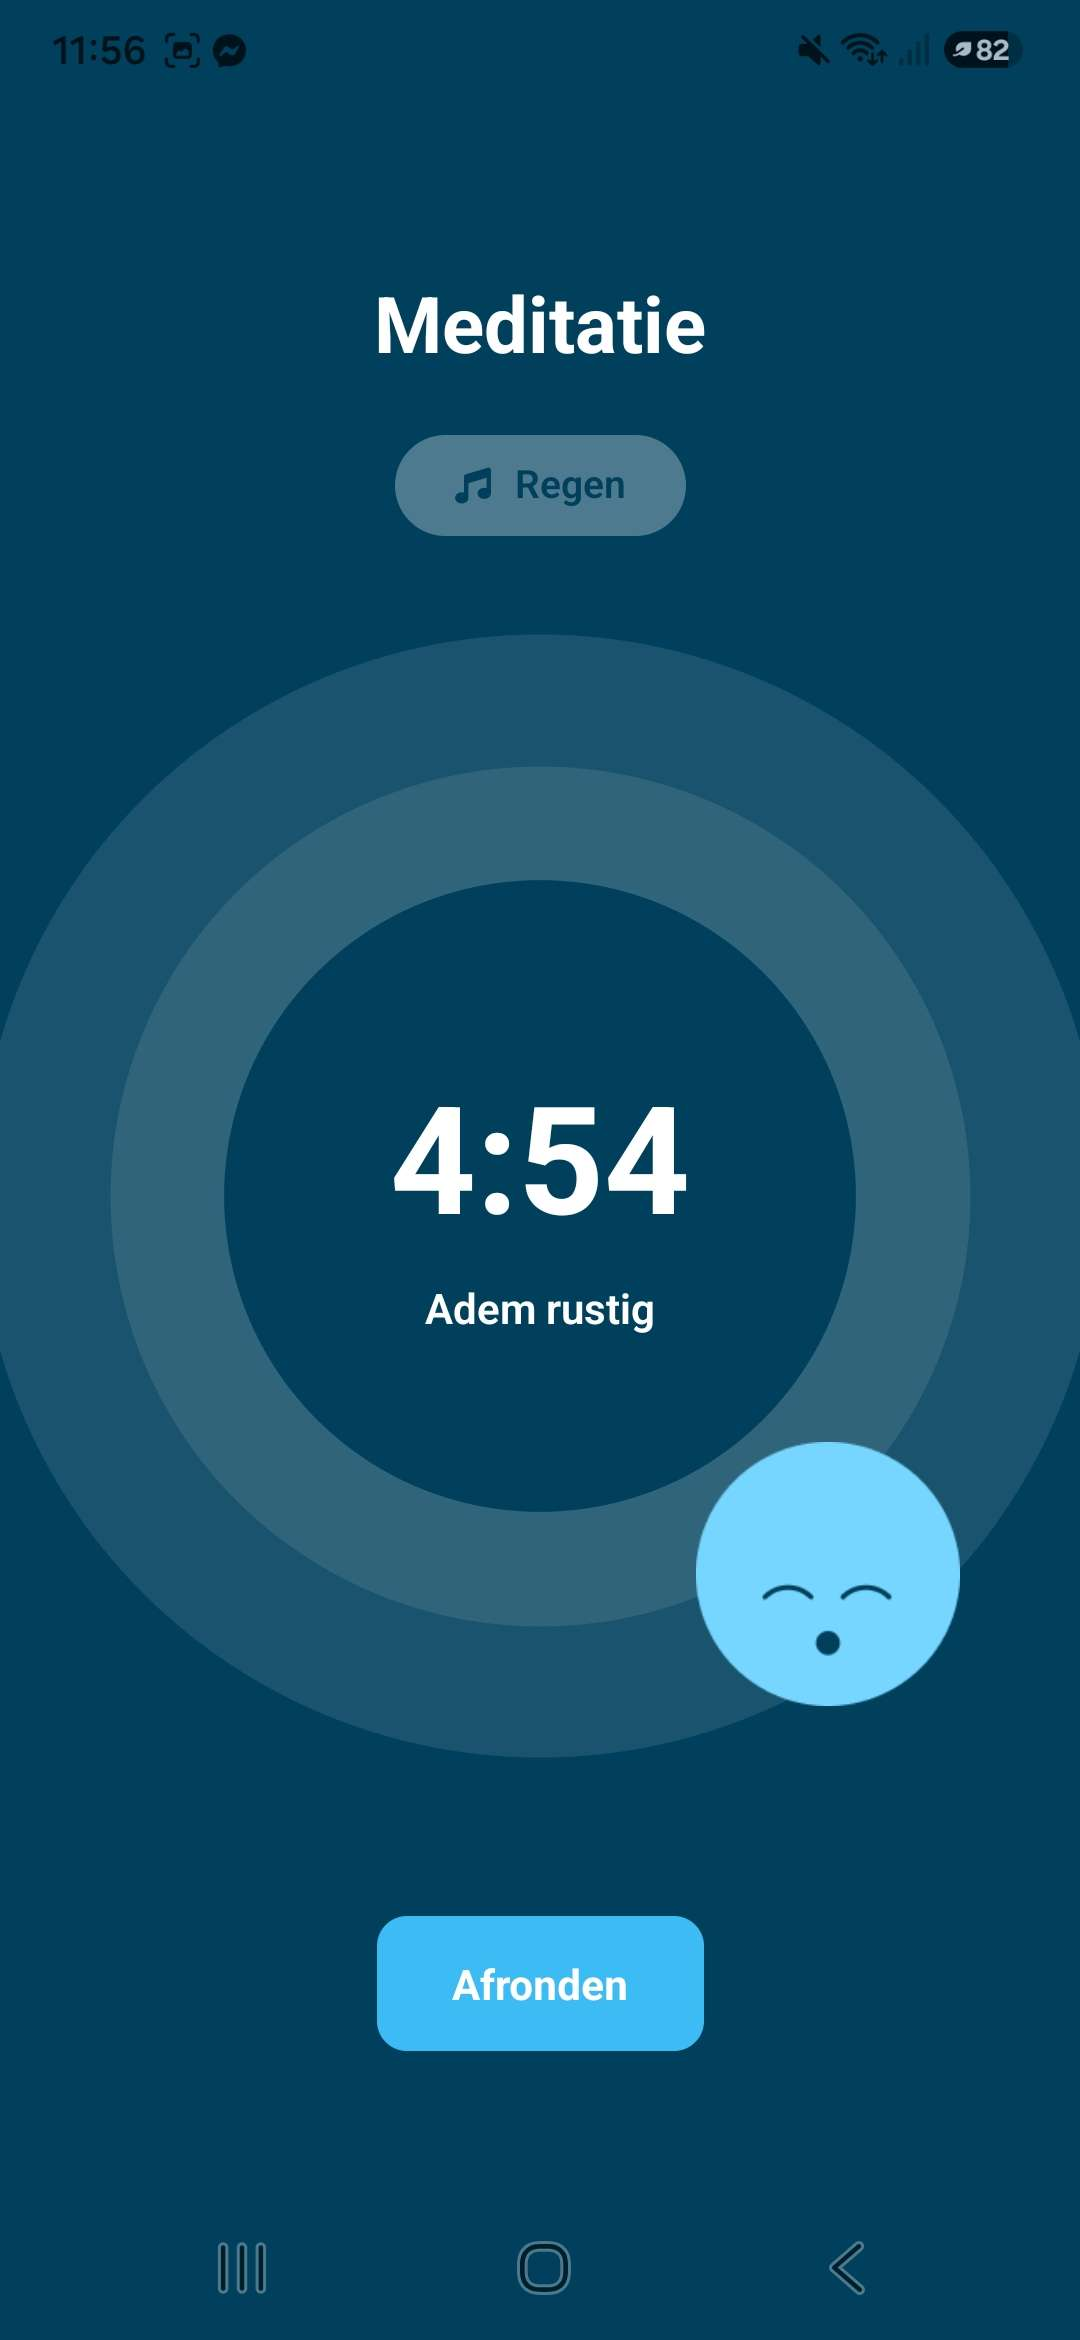
\includegraphics[width=\linewidth]{../graphics/Code/PoC23}
    \end{minipage}
    \hfill
    \begin{minipage}{0.3\textwidth}
        \centering
        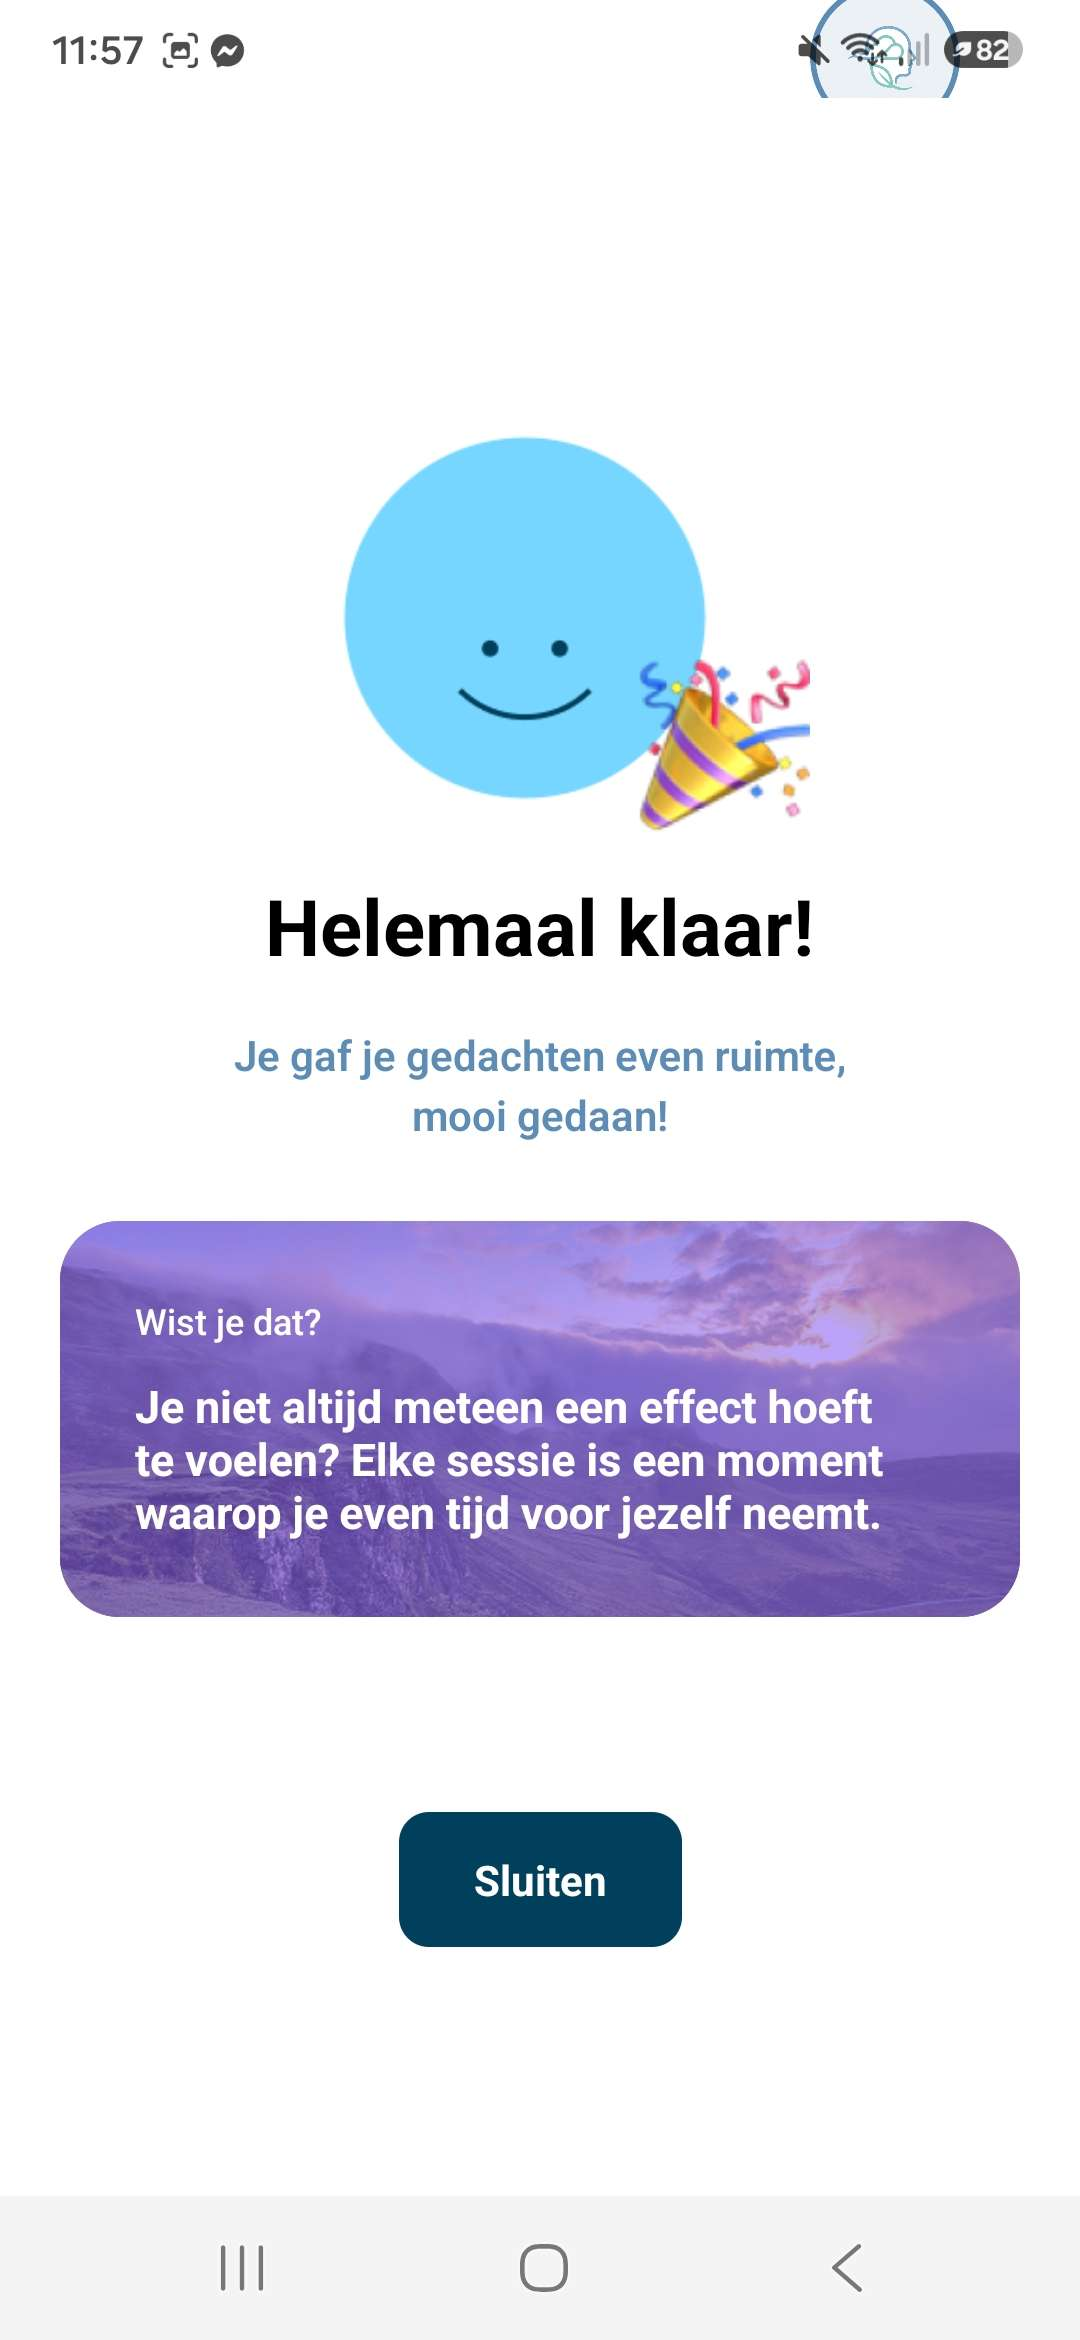
\includegraphics[width=\linewidth]{../graphics/Code/PoC24}
    \end{minipage}
    
    \caption{Vervolg en afronding van de reflectiefunctie en een voorbeeld van een begeleide meditatieoefening.}
    \label{fig:code-ss-4}
\end{figure}
